% Plantilla TFG LaTeX LSI por:
%   Agustín Borrego <borrego@us.es>
%   Inma Hernández <inmahernandez@us.es>
% Su uso y modificación es libre.

% ̀¡Recuerda hacer copias de seguridad frecuentes durante la redacción del trabajo!
% Puedes descargar todo el código fuente del proyecto en zip en Menú > (Descargar) Fuente

\documentclass[12pt]{report}

% Paquetes LaTeX y estilos globales
\usepackage[utf8]{inputenc}
\usepackage{multicol}
\usepackage{xcolor}
\usepackage{subfigure}
\usepackage[spanish,es-tabla]{babel}
\usepackage[utf8]{inputenc}
\usepackage{graphicx}
\usepackage{titlesec}
\usepackage[bookmarks,breaklinks,colorlinks=true,allcolors=blue]{hyperref}
\usepackage{listings}
\usepackage{inconsolata}
\usepackage{float}
% \usepackage{mathpazo} % Fuente Palatino -- comentado SOLO para preview local (falta el paquete "palatino" en tu BasicTeX). Descomentar al usar Overleaf, o tras "sudo tlmgr install palatino".
\usepackage[labelfont=bf]{caption}

\usepackage[square,numbers]{natbib}
\usepackage[nottoc,notlof,notlot]{tocbibind}  % Mete la bibliografía como capítulo en la TOC, los parámetros excluyen los otros índices de aparecer también
\usepackage{geometry}
\usepackage{amsmath}
\usepackage{amssymb} % \checkmark, entre otros símbolos usados en tablas
\usepackage{booktabs} % Estilo de tablas con \toprule/\midrule/\bottomrule
\usepackage{colortbl} % \rowcolor, \cellcolor -- cabeceras de tabla resaltadas
\usepackage{multirow} % Celdas que ocupan varias filas en tablas (p.ej. agrupar hiperparámetros por algoritmo)
\usepackage{longtable} % Tablas de cuadrícula completa que pueden partirse entre páginas
\usepackage{array} % Modificadores de columna (p.ej. centrado en columnas p{}) en tablas
\usepackage{tikz} % Diagramas EDT y de arquitectura dibujados directamente en LaTeX
\usetikzlibrary{arrows.meta} % Puntas de flecha modernas (p.ej. -{Latex[...]}) en los diagramas tikz
\usetikzlibrary{calc} % Coordenadas calculadas (p.ej. punto medio entre dos nodos) en los diagramas tikz
\usetikzlibrary{shapes.geometric} % Elipses (nodos de caso de uso UML) en los diagramas tikz
\usepackage[section]{placeins} % Fuerza a colocar todas las tablas/figuras pendientes antes de cada nueva sección, evitando que "adelanten" al texto siguiente
\usepackage{parskip}
\usepackage[official]{eurosym}
\usepackage{todonotes}
\usepackage{csquotes}
\usepackage{tocbasic}  % Estilos de la TOC

\input{etc/style}

%%%%%%%%%%%%%%%%%%%%%%%%%%%%%%%%%%%%%%%%%%%%%%%%%%%%%%%%%%%%%%%%%%%%%%%%%%%%%%%%%%%%%

% Variables para la portada
\setTitle{Visión artificial aplicada a partidos de fútbol utilizando el dataset SoccerNet}
\setAuthor{Carlos Galea Magro} % Si hay más de un autor, separarlos con \\
\setDegree{Grado en Ingeniería Informática - Ingeniería del Software} % Cambiar si es necesario
\setSupervisor{Manuel Carranza García} % Si hay más de un tutor, separarlos con \\
\setDepartment{Lenguajes y Sistemas Informáticos}
\setMonth{octubre} % Dejar sólo el mes de la convocatoria en que se presenta el trabajo
\setYear{2025/26} % Por ejemplo, 2022/23

%%%%%%%%%%%%%%%%%%%%%%%%%%%%%%%%%%%%%%%%%%%%%%%%%%%%%%%%%%%%%%%%%%%%%%%%%%%%%%%%%%%%%

% Dedicatoria del trabajo
 %Si no se desea incluir, comentar o borrar la línea siguiente para eliminar la página de dedicatoria
% \setDedication{Aquí la dedicatoria del trabajo}

%%%%%%%%%%%%%%%%%%%%%%%%%%%%%%%%%%%%%%%%%%%%%%%%%%%%%%%%%%%%%%%%%%%%%%%%%%%%%%%%%%%%%

% Comienzo del documento
\begin{document}

    % Portada y secciones no numeradas
    \input{sections/00_portada}
    \chapter*{Agradecimientos}

Este proyecto significa mucho para mí y pone fin a una etapa de mi vida. Este marca el fin de mis estudios
de grado. Por ello, me gustaría empezar a dar las gracias a todos los que han hecho posible llegar hasta este
punto.

Empezando por mi familia, mis padres y mi hermano siempre estuvieron ahí, me aconsejaron y recibí su apoyo en todo momento durante
esta etapa además de demostrarme la importancia de tener un buen equilibrio entre la vida personal y profesional.
A mis abuelos y mi tía, que así como mis padres me apoyaron y me dieron la educación y la importancia de ser constante para conseguir lo que quieres.

A mis amigos de la universidad, con los que he compartido buenos momentos y han hecho que esta etapa sea amena y divertida a la vez que un reto.
Muchos momentos fueron más fáciles durante la carrera gracias a ellos, ya que nos ayudábamos mutuamente.

A mi experiencia de Erasmus este último año, donde conocí a muchos amigos que me han apoyado, pero sobre todo, esta experiencia me ha ayudado
a crecer como persona: tanto por las amistades como por mí mismo, me hizo cambiar mi forma de ver el mundo y abrir mi mente.

También quiero agradecer a Manuel Carranza, que ha sido quien me ha ayudado y guiado en este proyecto por su dedicación, haciéndolo posible.

    \chapter*{Resumen}

El seguimiento multiobjeto (\emph{multi-object tracking}, MOT) de jugadores
en vídeo de fútbol es un paso previo necesario para cualquier análisis
automático del juego como mapas de calor, distancia recorrida, posesión de
balón, pero elegir un algoritmo concreto para esa tarea exige compararlo
sobre datos reales de fútbol y no solo sobre los benchmarks genéricos de
seguimiento de personas para los que se diseñó originalmente. Este Trabajo
de Fin de Grado aborda esa comparación sobre SoccerNet-Tracking, un
\emph{dataset} público de vídeo de fútbol con detecciones precomputadas, y
propone un sistema completo que va desde el seguimiento hasta la
extracción de metadatos deportivos interpretables a partir de las
trayectorias resultantes.

El sistema compara dos algoritmos de
asociación clásicos, ByteTrack y OC-SORT, evaluados con las métricas
estándar de TrackEval (HOTA, MOTA, IDF1) sobre los conjuntos de
entrenamiento y de test. Sobre la configuración óptima de cada algoritmo,
obtenida mediante un estudio sistemático de hiperparámetros, se construye
un segundo pipeline de extracción de metadatos: clasificación de equipos
por color de camiseta mediante K-means, mapas de calor de posiciones,
distancia y velocidad reales a partir de una homografía calibrada
manualmente, y posesión de balón por proximidad. Los resultados, junto con
vídeos anotados, se exponen finalmente en una aplicación web.

El conjunto de datos procesado reúne 106 secuencias de vídeo (57 de
entrenamiento, 49 de test) de 700 fotogramas cada una y con
detecciones precomputadas de jugadores, árbitros y balón. Con la métrica
HOTA(0) (evaluada en un único umbral),
ByteTrack alcanza 81,43 en test frente a 80,92 de OC-SORT; sin embargo,
con la métrica HOTA integrada estándar el resultado se invierte con
claridad en ambos conjuntos (80,23 frente a 73,27 en entrenamiento; 75,43
frente a 70,73 en test), porque OC-SORT reutiliza las detecciones del
\emph{dataset} sin modificarlas mientras que ByteTrack sí las interpola en
su segunda ronda de asociación. Esta discrepancia, documentada y explicada
en detalle en la memoria, es uno de los resultados más relevantes del
trabajo: dos formas igual de legítimas de medir el mismo sistema pueden
llevar a conclusiones opuestas sobre qué algoritmo es mejor.

\vspace{.5cm}

\textbf{Palabras clave:} SoccerNet, Seguimiento Multiobjeto, Visión
Artificial, ByteTrack, OC-SORT, HOTA, Análisis Deportivo.

    \chapter*{Abstract}

Multi-object tracking (MOT) of players in football video is a necessary
prerequisite for any automatic analysis of the game, such as heatmaps,
distance covered or ball possession, but choosing a specific algorithm for
that task requires comparing it on real football data rather than only on
the generic person-tracking benchmarks it was originally designed for.
This Final Degree Project addresses that comparison on SoccerNet-Tracking,
a public football video dataset with precomputed detections, and proposes
a complete system that goes from tracking to the extraction of
interpretable sports metadata from the resulting trajectories.

The system compares two classic association algorithms, ByteTrack and
OC-SORT, evaluated with the standard TrackEval metrics (HOTA, MOTA, IDF1)
on the training and test sets. On top of the optimal configuration of each
algorithm, obtained through a systematic hyperparameter study, a second
metadata extraction pipeline is built: team classification by jersey
colour using K-means, position heatmaps, real distance and speed from a
manually calibrated homography, and ball possession by proximity. The
results, together with annotated videos, are finally presented in a web
application.

The processed dataset gathers 106 video sequences (57 training, 49 test)
of 700 frames each, with precomputed detections of players, referees and
the ball. Using the HOTA(0) metric (evaluated at a single overlap
threshold), ByteTrack reaches 81.43 on test versus 80.92 for OC-SORT;
however, under the standard integrated HOTA metric the result is clearly
reversed on both sets (80.23 versus 73.27 on training; 75.43 versus 70.73
on test), because OC-SORT reuses the dataset detections unmodified while
ByteTrack interpolates them in its second association round. This
discrepancy, documented and explained in detail in the report, is one of
the most relevant results of the project: two equally legitimate ways of
measuring the same system can lead to opposite conclusions about which
algorithm is better.

\vspace{.5cm}

\textbf{Keywords:} SoccerNet, Multi-Object Tracking, Computer Vision,
ByteTrack, OC-SORT, HOTA, Sports Analytics.

    
    % Índice del documento y de figuras
    \begingroup
        % Los enlaces son normalmente azules, pero en los índices se configuran a negro para que no aparezca todo azul
        \hypersetup{linkcolor=black}
        \tableofcontents
        \listoffigures
        \listoftables
        \lstlistoflistings
    \endgroup
    
    % Cambia el estilo de números de página de romanos a normal
    \clearpage\pagenumbering{arabic}
    
    % Capítulos del trabajo
    % \input{sections/ejemplos_borrame} % capítulo de ejemplos de la plantilla, no forma parte de la memoria final
    \chapter{Introducción}
\label{cap:introduccion}

\section{Motivación}
\label{sec:intro-motivacion}

El análisis de datos es una disciplina de la informática que me apasiona, así como
el deporte. El análisis de datos aplicado al deporte ha experimentado un crecimiento notable
en la última década. Clubes, televisión, casas de apuestas y compañías de análisis
deportivo invierten cada vez más recursos en extraer información objetiva del
juego a partir del vídeo: distancias recorridas, mapas de calor,
patrones tácticos o detección automática de eventos. Gran parte de esta
información depende de una tarea previa fundamental: saber, en cada instante,
dónde está cada jugador y quién es. Partiendo de esa base, posteriormente se
pueden calcular distintas métricas de interés para el análisis del partido.

Ese problema, conocido en visión por computador como \emph{seguimiento
multiobjeto} o \emph{Multi-Object Tracking} (MOT), es especialmente exigente
en un partido de fútbol: veintidós jugadores más árbitros y balón se mueven de
forma simultánea, se cruzan constantemente, se ocluyen entre sí y comparten
una apariencia muy similar entre compañeros de equipo (misma camiseta, tallas
y complexiones parecidas). Estas condiciones convierten al fútbol en un
escenario particularmente duro para evaluar algoritmos de tracking, mucho más
que los entornos de vigilancia urbana o conducción autónoma para los que
originalmente se diseñaron muchos de estos algoritmos.

Este proyecto nace de aplicar y comparar de forma rigurosa
algoritmos de seguimiento multiobjeto sobre vídeo real de partidos de fútbol
profesional, y comprobar hasta qué punto la información de trayectorias que
producen puede convertirse en metadatos deportivos útiles, sin necesidad de instrumentación adicional
en el terreno de juego, únicamente a partir del vídeo.

\section{Contexto}
\label{sec:intro-contexto}

SoccerNet es un conjunto de datos y una serie de competiciones académicas
centradas en el análisis automático de vídeo de fútbol, con múltiples tareas
publicadas (reconocimiento de acciones, segmentación de cámara, reconocimiento
de dorsales, seguimiento de jugadores, entre otras). Este proyecto se apoya en
la tarea \textbf{SoccerNet-Tracking}, que proporciona secuencias de vídeo de
partidos profesionales descompuestas en frames individuales, junto con
detecciones de personas y balón ya calculadas (\texttt{det.txt}) y, para los
conjuntos de entrenamiento y test, la posición e identidad real de cada
jugador en cada frame (\texttt{gt.txt}), que sirve como referencia para medir
el rendimiento de los algoritmos.

El uso de un dataset público y con un formato estándar permite que los resultados obtenidos en
este proyecto sean comparables con los de otros equipos de investigación, y
que la evaluación se realice con las mismas métricas que utiliza la propia
comunidad de SoccerNet en su tabla de clasificación oficial.

\section{El problema}
\label{sec:intro-problema}

El seguimiento multiobjeto consiste en asignar, a cada objeto detectado en un
vídeo, una identidad que se mantenga consistente a lo largo de todos los
frames en los que ese objeto sea visible, incluso cuando desaparece
temporalmente de la imagen, por ejemplo, al quedar oculto detrás de otro
jugador y vuelve a aparecer poco después. Un buen algoritmo de tracking debe
resolver simultáneamente dos problemas relacionados pero distintos:

\begin{itemize}
  \item \textbf{Detección}: encontrar dónde está cada objeto de interés en
        cada frame. En este proyecto, jugadores, árbitros y balón.
  \item \textbf{Asociación}: decidir qué detección de un frame corresponde a
        qué identidad ya existente de un frame anterior, o si se trata de un
        objeto nuevo.
\end{itemize}

Es importante delimitar aquí, desde el principio, el alcance exacto de este
proyecto: el dataset SoccerNet-Tracking proporciona las detecciones ya
calculadas para cada frame (\texttt{det.txt}). Por tanto, la tarea abordada es
específicamente la de \textbf{asociación}: mantener identidades
consistentes a partir de un conjunto de detecciones dado y no la de
detección de jugadores desde cero a partir de la imagen. Esta
decisión, natural dado el planteamiento del dataset, permite centrar el
esfuerzo y la comparativa en los algoritmos de tracking propiamente dichos
(el componente de asociación), que es donde reside la principal diferencia
entre los distintos métodos evaluados. Esta distinción se retoma con más
detalle en el capítulo~\ref{cap:analisis}.

\section{Objetivos}
\label{sec:intro-objetivos}

\subsection{Objetivo general}

Una vez definidas las detecciones del dataset SoccerNet, se propone evaluar y comparar distintos algoritmos de seguimiento multiobjeto sobre
secuencias reales de partidos de fútbol del dataset SoccerNet, y explorar
en qué medida las trayectorias resultantes permiten extraer metadatos
deportivos de utilidad para el análisis de un partido.

\subsection{Objetivos específicos}

A partir de este objetivo general se han definido los siguientes objetivos
específicos:

\begin{itemize}
  \item \textbf{OE-01:} Estudiar la estructura del dataset
        SoccerNet-Tracking (secuencias de frames, detecciones precomputadas
        y \emph{ground truth}) y delimitar la tarea abordada como un
        problema de asociación en mayor medida que de detección.
  \item \textbf{OE-02:} Implementar varios algoritmos de tracking de tipo
        \emph{tracking-by-detection}, incluyendo un
        filtrado geométrico que separe el balón de los jugadores antes de
        la asociación.
  \item \textbf{OE-03:} Ejecutar los algoritmos escogidos (\textbf{ByteTrack} y
        \textbf{OC-SORT}) sobre la totalidad de las
        secuencias de los conjuntos de entrenamiento y de test del dataset.
  \item \textbf{OE-04:} Evaluar ambos algoritmos con las métricas estándar
        del campo (HOTA, MOTA, IDF1) mediante \texttt{TrackEval}, comparando
        su comportamiento entre el conjunto de entrenamiento y el de test.
  \item \textbf{OE-05:} Realizar un estudio sistemático de hiperparámetros
        de cada algoritmo, variando un parámetro a la vez, y determinar una
        configuración óptima para cada uno de ellos.
  \item \textbf{OE-06:} Diseñar y aplicar un método de clasificación de
        jugadores por equipo a partir del color dominante de la camiseta
        mediante K-means.
  \item \textbf{OE-07:} Generar mapas de calor de ocupación del campo a
        partir de las trayectorias obtenidas, tanto de forma global como
        separados por equipo.
  \item \textbf{OE-08:} Calcular una homografía real sobre tramos de vídeo
        con cámara estable, como prueba de concepto para estimar la
        distancia recorrida y la velocidad de los jugadores en unidades
        reales.
  \item \textbf{OE-09:} Estimar la posesión del balón por proximidad
        espacial entre el balón y el jugador más cercano, y si es posible, 
        generar un resumen de posesión de balón por jugador y
        agregarla por equipo.
  \item \textbf{OE-10:} Documentar las limitaciones
        técnicas encontradas en cada etapa del proyecto, incluyendo
        enfoques explorados y descartados, de modo que la memoria refleje
        fielmente tanto lo conseguido como las dificultades reales del
        proceso.
  \item \textbf{OE-11:} Desarrollar una aplicación web que sirva como
        demostrador visual e interactivo de los resultados del proyecto obtenidos,
        permitiendo explorar los
        resultados de tracking y el análisis de datos generado. También se
        destinada a personas que no sean expertas en el área para facilitar
        su comprensión y visualización.
\end{itemize}

\section{Alcance y delimitación del proyecto}
\label{sec:intro-alcance}

Como se ha introducido en la sección~\ref{sec:intro-problema}, este proyecto
parte de las detecciones del dataset y se centra en la etapa de
asociación (tracking), no en el diseño de un detector de objetos propio. Estos son
 los límites principales del proyecto:

\begin{itemize}
  \item Los algoritmos comparados corresponden a la familia de métodos
        \emph{tracking-by-detection} clásicos, los usados no tienen componente de
        reidentificación visual profunda (\emph{re-ID}) pero la incorporación de
        algoritmos con re-ID se plantea como posible ampliación
        (capítulo~\ref{cap:conclusiones}).
  \item La proyección de posiciones de píxel a coordenadas reales del campo
        se realiza mediante dos enfoques de distinta fiabilidad: una
        aproximación por rango observado, usada
        de forma general, y una homografía real calculada manualmente sobre
        tramos concretos con cámara estable, usada como prueba de concepto
        para el cálculo de distancia y velocidad. Ambos enfoques, y sus
        limitaciones, se detallan en el capítulo~\ref{cap:implementacion}.
  \item La posesión del balón se estima por proximidad espacial entre el
        balón detectado y el jugador más cercano, una aproximación razonable
        pero distinta del concepto de posesión que manejaría un analista
        táctico humano.
\end{itemize}

\section{Estructura del documento}
\label{sec:intro-estructura}

La memoria de este proyecto se organiza en los siguientes capítulos:

\begin{itemize}
  \item \textbf{Capítulo~\ref{cap:fundamentos} -- Fundamentos teóricos y
        estado del arte.}
        Describe los conceptos teóricos necesarios para entender el
        proyecto y el estado del arte. Explica el problema del seguimiento multiobjeto, los algoritmos
        de tracking comparados, las métricas de evaluación empleadas, la
        clasificación de jugadores por color y los fundamentos de la
        homografía entre otros. y por último, cierra situando este TFG frente a los
        resultados del reto oficial de SoccerNet.
  \item \textbf{Capítulo~\ref{cap:gestion} -- Gestión del proyecto.}
        Describe la metodología de trabajo seguida, la planificación
        temporal, la estructura de descomposición del trabajo, y una
        estimación de los recursos y costes que habría requerido este
        proyecto en un contexto profesional.
  \item \textbf{Capítulo~\ref{cap:analisis} -- Análisis de requisitos.}
        Recoge los actores del sistema, los requisitos de información,
        funcionales y no funcionales, las reglas de negocio y los casos de
        uso.
  \item \textbf{Capítulo~\ref{cap:diseno} -- Diseño.}
        Presenta la arquitectura general del sistema y las decisiones de
        diseño tomadas.
  \item \textbf{Capítulo~\ref{cap:implementacion} -- Implementación.}
        Detalla cómo se han implementado el tracking, la evaluación, el
        estudio de hiperparámetros, el pipeline de metadatos y la
        aplicación web, tambien los problemas técnicos encontrados y los
        enfoques que se probaron y no funcionaron.
  \item \textbf{Capítulo~\ref{cap:pruebas} -- Resultados.}
        Recoge la comparativa final entre ByteTrack y OC-SORT, los
        resultados del estudio de hiperparámetros y del pipeline de
        metadatos, y las limitaciones detectadas en cada uno.
  \item \textbf{Capítulo~\ref{cap:manual} -- Manual de despliegue.}
        Explica paso a paso cómo instalar, configurar y ejecutar el
        sistema, incluida la aplicación web.
  \item \textbf{Capítulo~\ref{cap:uso-ia} -- Uso de inteligencia
        artificial.} Detalla el uso realizado de herramientas de
        inteligencia artificial durante el desarrollo del proyecto.
  \item \textbf{Capítulo~\ref{cap:conclusiones} -- Conclusiones y trabajo
        futuro.} Resume las
        conclusiones del proyecto y plantea posibles líneas futuras de
        trabajo.
\end{itemize}

Tras la bibliografía se incluye un glosario
con los términos y las siglas usadas a lo largo de la memoria.

    \chapter{Fundamentos teóricos y estado del arte}
\label{cap:fundamentos}

Este capítulo presenta los conceptos
teóricos necesarios para comprender el resto del proyecto. Se parte de
las nociones más básicas: qué es la inteligencia artificial, qué es un
dataset y por qué existe SoccerNet. Y se profundiza progresivamente llegando a
 cada algoritmo, métrica y técnica empleados: el
problema del seguimiento multiobjeto, los algoritmos de \emph{tracking-by-detection}
comparados y los que se consideraron pero no llegaron
a implementarse, las métricas de evaluación estándar (MOTA, IDF1,
HOTA), la clasificación de jugadores por color y los
fundamentos de la homografía aplicada a la proyección de coordenadas.
Las decisiones de este proyecto como parámetros, configuración,
qué resultado se obtuvo se abordan en los capítulos de
diseño, implementación y resultados
(capítulos~\ref{cap:diseno},~\ref{cap:implementacion} y~\ref{cap:pruebas}).
El capítulo se cierra situando este TFG frente a trabajos relacionados y al
reto oficial de SoccerNet (sección~\ref{sec:fundamentos-relacionados}).

\section{Inteligencia artificial, aprendizaje automático y visión por computador}
\label{sec:fundamentos-ia}

La \textbf{inteligencia artificial} (IA) es el
campo de la informática dedicado a construir sistemas y programas capaces de realizar
tareas que normalmente requerían de la inteligencia humana, como el aprendizaje, el razonamiento y la percepción
\citep{gobiernoespana2023ia}.
Estas tareas incluyen reconocer un objeto en una imagen, entender una frase o
decidir la mejor ruta en un mapa. Dentro de ese campo tan amplio, el
\textbf{aprendizaje automático} (\emph{machine learning}) es el subconjunto
de la IA que no programa explícitamente la solución a un problema, sino que
la \emph{aprende} a partir de los patrones presentes en los datos de
entrenamiento, para después aplicar lo aprendido sobre datos nuevos
\citep{ibm2026ml}: en lugar de escribir a mano las
reglas que distinguen un gato de un perro en una fotografía, se le muestran
al sistema miles de fotografías etiquetadas y es el propio sistema el que
extrae, mediante un proceso de optimización, los patrones que le permiten
generalizar a fotografías nuevas que no ha visto antes.

Dentro del aprendizaje automático, el \textbf{aprendizaje profundo}
(\emph{deep learning}) es el subconjunto de técnicas basadas en redes
neuronales artificiales de varias capas, cuyo diseño se inspira de forma
general en la estructura del cerebro humano, capaces de aprender
directamente representaciones útiles de los datos en bruto sin necesidad de que un experto humano diseñe a
mano las características relevantes; es este subcampo el que sostiene hoy
la mayor parte de los avances más recientes de la IA, desde la visión
artificial y la IA generativa hasta la conducción autónoma o la robótica
\citep{ibm2026dl}. Es precisamente en visión artificial donde el
aprendizaje profundo ha hecho posibles, en la última década, los avances
más visibles: la \textbf{visión por computador} es la disciplina que
estudia cómo dotar a una máquina de la capacidad de procesar, analizar e
interpretar información significativa a partir de imágenes o vídeo
\citep{ibm2026cv}, y de ella forman parte tanto la detección de objetos
(encontrar dónde está cada objeto en una imagen) como el seguimiento
multiobjeto, tarea de este proyecto que se define formalmente en la
sección~\ref{sec:fundamentos-mot}.

\begin{figure}[htp]
\centering
\begin{tikzpicture}[
  every node/.style={align=center, font=\small},
  box/.style={draw, rounded corners, minimum height=1.4cm}
]
\node[box, fill=gray!10, minimum width=11cm, minimum height=6.2cm, anchor=north] (ia) at (0,3) {};
\node[align=center] at (0,2.7) {\textbf{Inteligencia artificial}};
\node[box, fill=blue!8, minimum width=8.6cm, minimum height=4.6cm, anchor=north] (ml) at (0,2.1) {};
\node[align=center] at (0,1.8) {\textbf{Aprendizaje automático}\\\footnotesize{(\emph{machine learning})}};
\node[box, fill=blue!18, minimum width=6.2cm, minimum height=3.0cm, anchor=north] (dl) at (0,1.0) {};
\node[align=center] at (0,0.7) {\textbf{Aprendizaje profundo}\\\footnotesize{(\emph{deep learning})}};
\node[box, fill=blue!30, minimum width=3.6cm, minimum height=1.3cm, anchor=north] (cv) at (0,-0.4) {};
\node[align=center] at (0,-0.7) {\footnotesize\textbf{Visión por}\\\footnotesize\textbf{computador}};
\end{tikzpicture}
\caption{Relación de contención entre inteligencia artificial, aprendizaje
automático, aprendizaje profundo y visión por computador. La visión por
computador se apoya hoy predominantemente en aprendizaje profundo, aunque
históricamente incluye también técnicas no basadas en redes neuronales
(por ejemplo, K-means, sección~\ref{sec:fundamentos-kmeans}).}
\label{fig:jerarquia-ia}
\end{figure}

El \textbf{análisis de datos} es, en paralelo, la disciplina que convierte
datos generados por sensores o, como en este proyecto,
algoritmos de visión por computador, en información interpretable: medias,
distribuciones, mapas de calor, tendencias o comparativas
\citep{coursera2026dataanalysis}. La intersección
de ambos campos es precisamente lo que estructura este proyecto: primero se
usa visión por computador para producir datos de trayectorias a partir de
vídeo (capítulos~\ref{cap:diseno} y~\ref{cap:implementacion}), y después se
aplica análisis de datos sobre esas trayectorias para obtener metadatos
deportivos interpretables (mapas de calor, distancias, posesión), como se
detalla en la sección~\ref{sec:implementacion-metadatos}.

\section{Datasets y el ecosistema SoccerNet}
\label{sec:fundamentos-dataset}

Todo sistema de aprendizaje automático necesita datos con los que aprender
y, sobre todo, con los que poder evaluarse de forma objetiva. Un
\textbf{dataset} (conjunto de datos) es, en este contexto, una colección
organizada de ejemplos (en visión por computador, típicamente imágenes o
vídeos) acompañados de anotaciones de referencia (\emph{ground truth}) que
indican cuál es la respuesta correcta para cada ejemplo
\citep{ibm2026dataset}. Un
\textbf{benchmark} es, además, un dataset acompañado de un protocolo de
evaluación estandarizado (qué métricas se calculan, cómo se dividen los
datos en entrenamiento y test) que permite comparar de forma justa los
resultados obtenidos por distintos investigadores o equipos, incluso años
después y sin que hayan trabajado nunca juntos. Sin datasets públicos con
estas características, cualquier comparación entre algoritmos, como la que
constituye el núcleo de este proyecto, carecería de validez: cada autor
podría estar evaluando sobre datos distintos, más favorables a su propio
método. MOTChallenge \citep{motchallengeweb2026} y el propio
SoccerNet-Tracking \citep{cioppa2022soccernettracking}, presentados a
continuación, son dos ejemplos concretos de este tipo de benchmark
aplicados al seguimiento multiobjeto.

\textbf{SoccerNet} \citep{soccernetweb2026} es un
ecosistema de datasets y competiciones académicas anuales centrado en el
análisis automático de vídeo de fútbol profesional, mantenido por un
consorcio de investigadores de varias universidades. Ofrece múltiples
tareas sobre el mismo conjunto de partidos de origen (reconocimiento de
acciones, segmentación del tipo de plano de cámara, reconocimiento del
dorsal del jugador, seguimiento multiobjeto, entre otras), cada una con su
propio subconjunto de datos, su propio formato de anotación y su propio
protocolo de evaluación. La sección~\ref{sec:analisis-decision} del
capítulo~\ref{cap:analisis} detalla el proceso de exploración de estas
tareas alternativas antes de decidirse por la tarea de tracking.

\subsection{SoccerNet-Tracking}
\label{subsec:fundamentos-soccernet-tracking}

Este proyecto se apoya específicamente en \textbf{SoccerNet-Tracking}
\citep{cioppa2022soccernettracking}, la tarea de seguimiento multiobjeto del
ecosistema SoccerNet. El dataset está compuesto por 200 secuencias de vídeo
de 30 segundos cada una, extraídas de partidos profesionales reales y
seleccionadas por representar situaciones de juego especialmente exigentes
para el tracking (aglomeraciones de jugadores, cambios bruscos de
dirección, oclusiones). Cada secuencia se distribuye ya descompuesta en
frames individuales (formato de imagen), en lugar de como un fichero de
vídeo, lo que facilita el procesamiento frame a frame que exigen los
algoritmos de tracking.

\begin{figure}[htp]
\centering
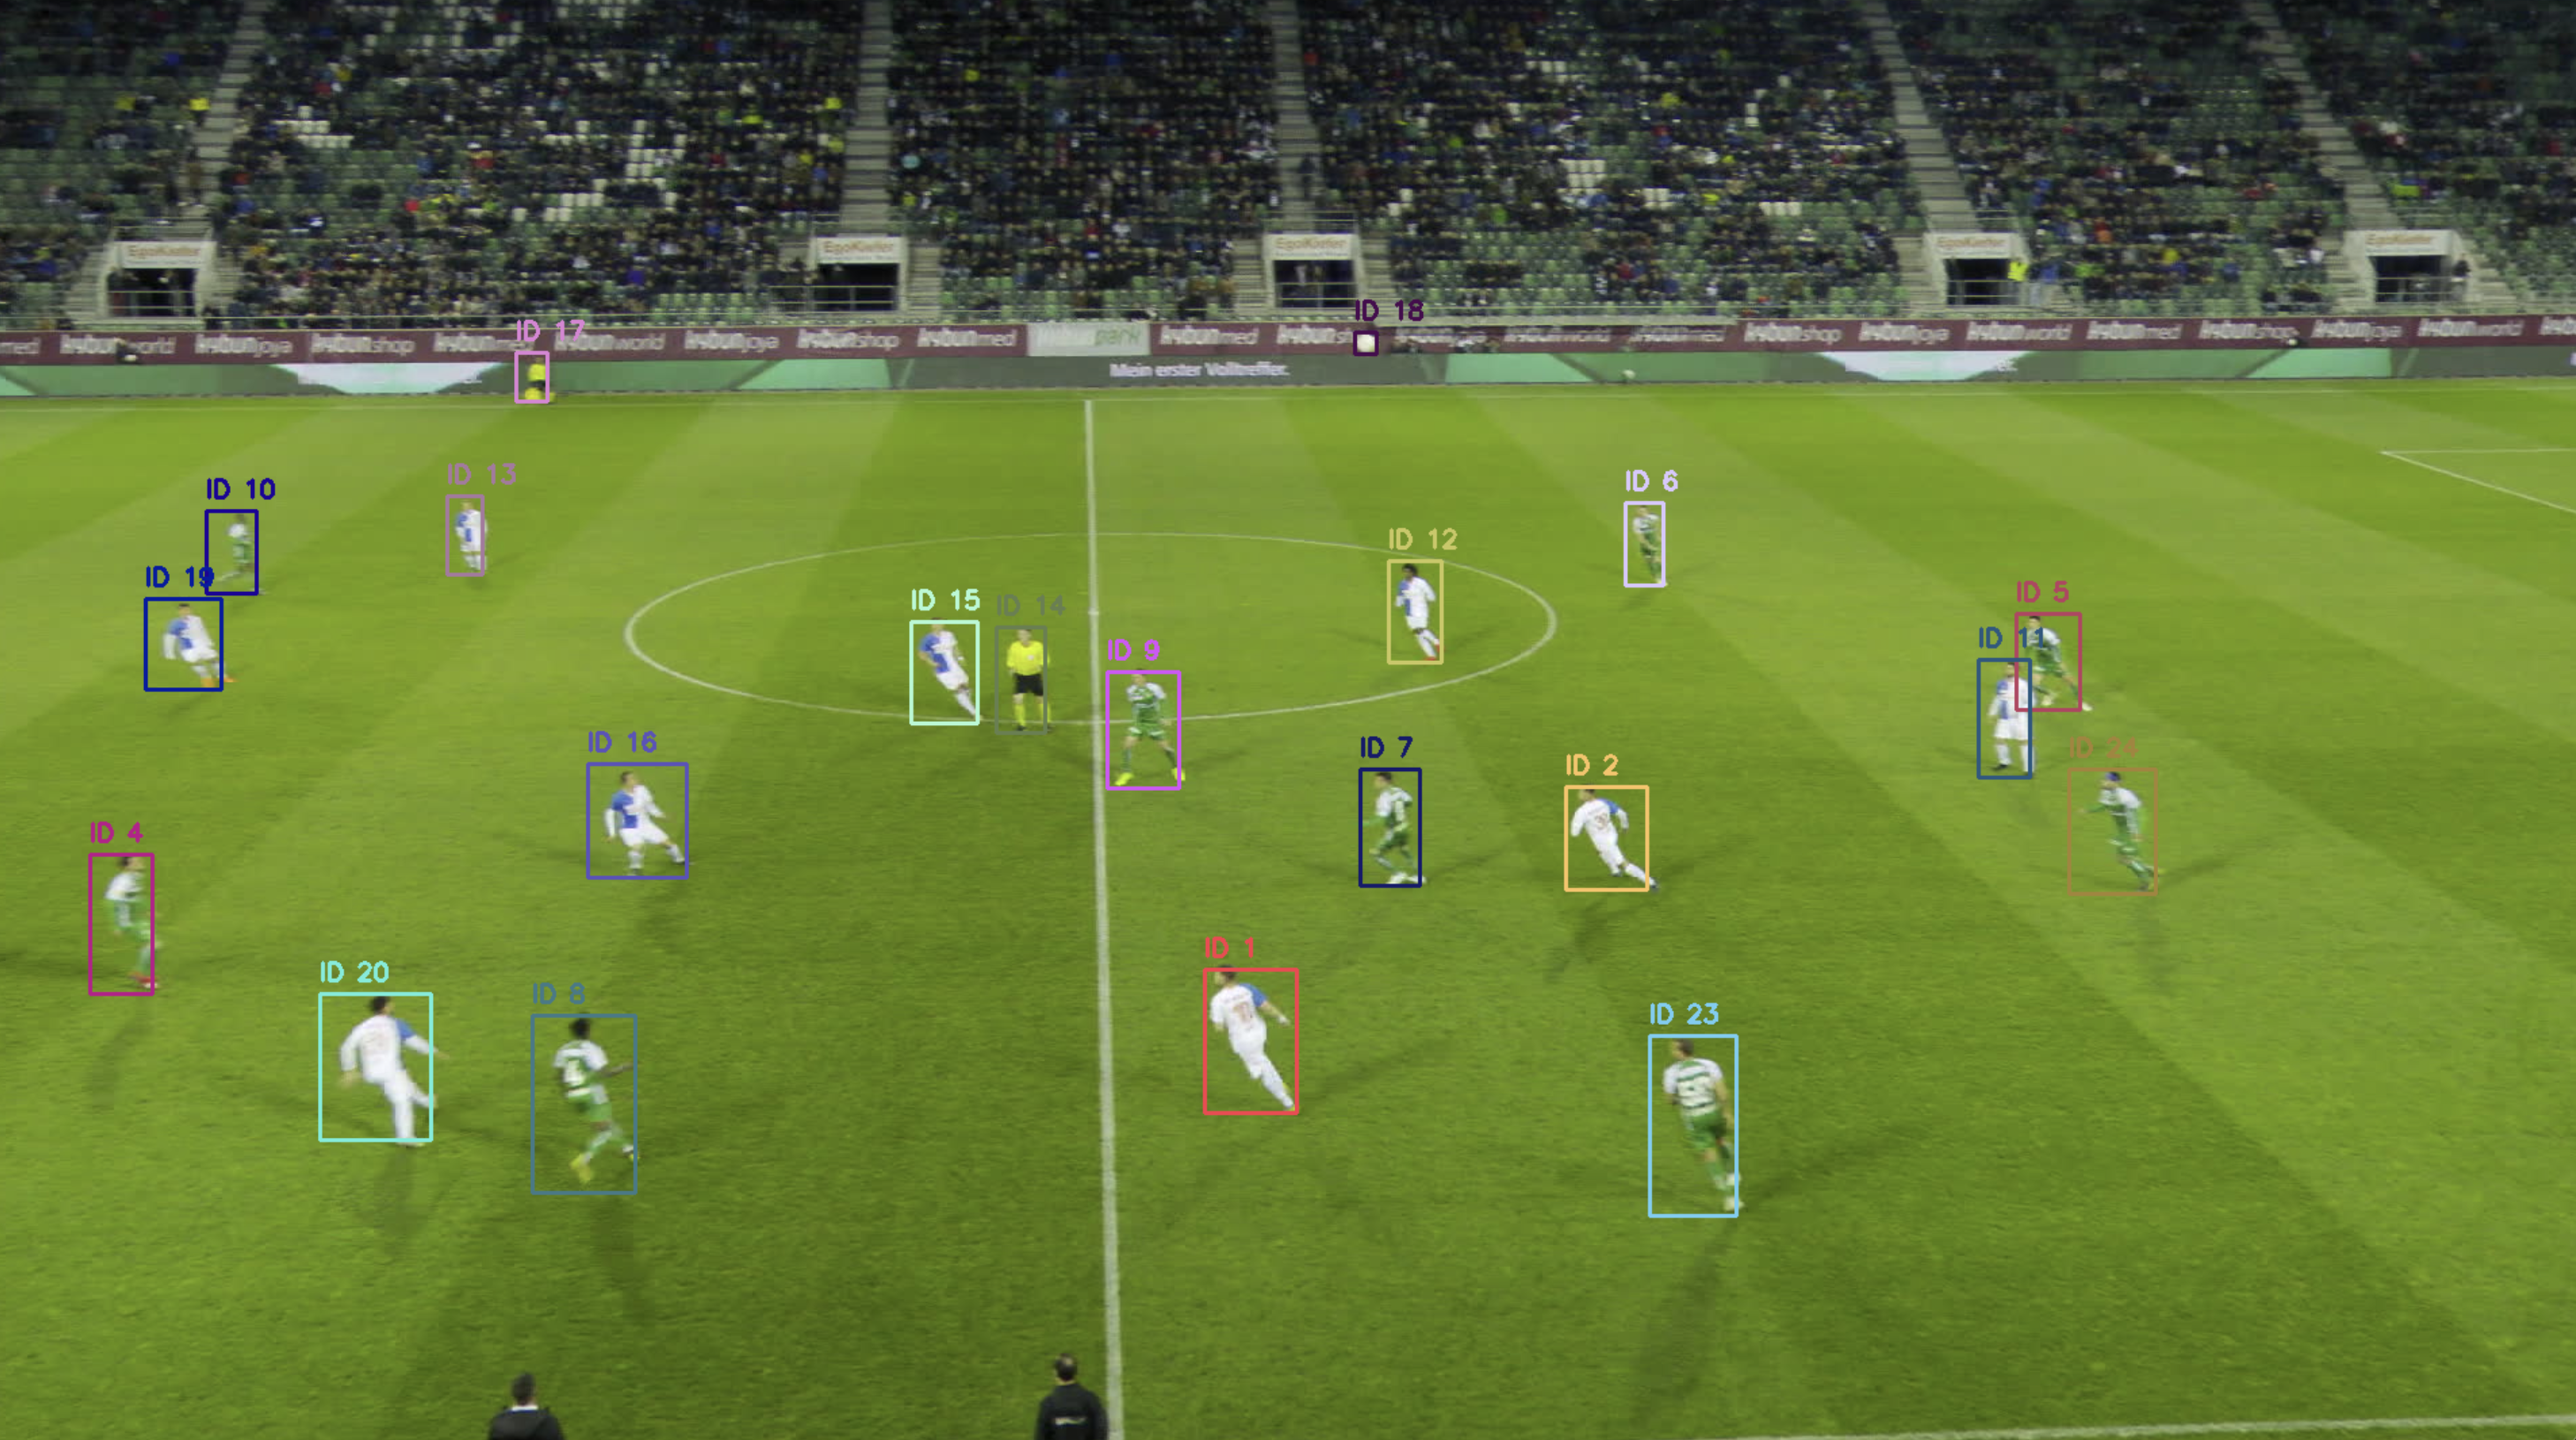
\includegraphics[width=0.92\textwidth]{figures/tracking-example.png}
\caption{Frame de una secuencia de SoccerNet-Tracking, con las cajas
delimitadoras y los identificadores de un resultado de tracking
superpuestos.}
\label{fig:tracking-example}
\end{figure}

Cada secuencia incluye, junto con los frames, los siguientes ficheros:

\begin{itemize}
  \item \textbf{\texttt{img1/}}: carpeta con los frames individuales de la
        secuencia, numerados de forma correlativa.
  \item \textbf{\texttt{det/det.txt}}: detecciones \emph{precomputadas} de
        cada objeto (jugadores, árbitros y balón) en cada frame, obtenidas
        con un detector de objetos ya entrenado por los organizadores del
        dataset. Esta es la entrada real de los algoritmos de tracking
        evaluados en este proyecto, como se explica en la
        sección~\ref{sec:fundamentos-mot}.
  \item \textbf{\texttt{gt/gt.txt}}: la posición e identidad
        \emph{real} de cada objeto en cada frame, usada como referencia
        para calcular las métricas de evaluación de la
        sección~\ref{sec:fundamentos-metricas}.
  \item \textbf{\texttt{seqinfo.ini}} y \textbf{\texttt{gameinfo.ini}}:
        metadatos de la secuencia (resolución de imagen, \emph{frame rate})
        y del partido de origen.
\end{itemize}

Tanto \texttt{det.txt} como \texttt{gt.txt} siguen el formato estándar del
protocolo \textbf{MOTChallenge} \citep{motchallengeweb2026},
el benchmark de referencia histórico en seguimiento multiobjeto (orientado
originalmente a vigilancia urbana de peatones, no a deporte), que
SoccerNet-Tracking reutiliza para que las herramientas de evaluación ya
existentes (en particular \texttt{TrackEval}, empleada en este proyecto
(sección~\ref{sec:implementacion-evaluacion})) funcionen sin
modificaciones. Cada línea de estos ficheros describe un objeto en un frame
concreto:

\begin{center}
\texttt{frame\_id, obj\_id, x, y, w, h, confianza, -1, -1, -1}
\end{center}

donde \texttt{frame\_id} identifica el frame, \texttt{obj\_id} identifica
al objeto (en \texttt{gt.txt}, su identidad real y consistente a lo largo
de toda la secuencia; en \texttt{det.txt}, este campo no se usa), y
\texttt{x, y, w, h} describen la posición y el tamaño de la caja
delimitadora (\emph{bounding box}) del objeto en píxeles, con
\texttt{(x, y)} la esquina superior izquierda. Los tres últimos campos,
fijos a \texttt{-1}, corresponden a información adicional (clase de objeto,
visibilidad) que MOTChallenge contempla para otros dominios pero que
SoccerNet-Tracking no utiliza.

El dataset se organiza en tres particiones o splits: un conjunto de
\textbf{entrenamiento} (57 secuencias, con gt.txt disponible,
usado para desarrollar y ajustar los algoritmos), un conjunto de
\textbf{test} (con gt.txt disponible, reservado para la evaluación
final y no consultado durante el ajuste, tal y como exige una evaluación
honesta) y un conjunto de \emph{\textbf{challenge}} (sin gt.txt,
usado únicamente para el ranking oficial de la competición SoccerNet, no utilizado
 en este proyecto).

\section{El problema del seguimiento multiobjeto}
\label{sec:fundamentos-mot}

El \textbf{seguimiento multiobjeto} (\emph{Multi-Object Tracking}, MOT)
consiste en asignar, a cada objeto de interés que aparece en un vídeo, una
identidad numérica que se mantenga consistente a lo largo de todos los
frames en los que ese objeto sea visible incluso si desaparece
temporalmente de la imagen, por ejemplo al quedar oculto detrás de otro
jugador, y reaparece poco después \citep{ultralytics2026track}. Un sistema de MOT completo resuelve,
en general, dos subproblemas relacionados pero conceptualmente distintos,
representados en la Figura~\ref{fig:fundamentos-mot-pipeline}:

\begin{enumerate}
  \item \textbf{Detección}: localizar dónde está cada objeto de interés en
        cada frame individual, sin ninguna noción de continuidad temporal,
        es decir, sin saber todavía si el objeto detectado en el frame
        $t$ es el mismo que se detectó en el frame $t-1$. Esta tarea se
        resuelve habitualmente con un detector de objetos entrenado con
        aprendizaje profundo (por ejemplo, la familia YOLO, discutida en la
        sección~\ref{subsec:fundamentos-balon}).
  \item \textbf{Asociación}: dado el conjunto de detecciones de cada frame,
        decidir qué detección del frame actual corresponde a qué identidad
        ya existente de frames anteriores, o si se trata de un objeto que
        aparece por primera vez. Este es el problema que resuelven
        específicamente los algoritmos de tracking comparados en este
        proyecto (sección~\ref{sec:fundamentos-algoritmos}).
\end{enumerate}

\begin{figure}[htp]
\centering
\begin{tikzpicture}[
  every node/.style={align=center, font=\small},
  box/.style={draw, rounded corners, fill=blue!10, minimum width=2.6cm, minimum height=1.1cm},
  arrow/.style={-{Latex[length=2.5mm]}, thick}
]
\node[box] (frame) {Frame de vídeo};
\node[box, right=1.4cm of frame] (det) {Detección\\\footnotesize{(dónde está)}};
\node[box, right=1.4cm of det] (asoc) {Asociación\\\footnotesize{(quién es)}};
\node[box, right=1.4cm of asoc] (id) {Identidades\\consistentes};
\draw[arrow] (frame) -- (det);
\draw[arrow] (det) -- (asoc);
\draw[arrow] (asoc) -- (id);
\node[align=center, font=\footnotesize] at ($(det)!0.5!(asoc) + (0,-1.3)$)
  {Este proyecto se centra únicamente en la asociación.};
\end{tikzpicture}
\caption{Las dos etapas de un sistema de MOT: detección y asociación.}
\label{fig:fundamentos-mot-pipeline}
\end{figure}

Como se explicó en la sección~\ref{sec:intro-problema}, este proyecto se
sitúa solo en la segunda mitad de ese proceso: dado que
SoccerNet-Tracking proporciona las detecciones ya calculadas en
\texttt{det.txt} (sección~\ref{subsec:fundamentos-soccernet-tracking}), la
tarea abordada es específicamente la asociación, también llamada
\emph{tracking-by-detection} en la literatura, por oposición a los métodos
de \emph{joint detection and tracking} que entrenan un único modelo capaz
de detectar y asociar a la vez. Esta decisión, natural dado el
planteamiento del dataset, es también la que sigue la comparativa oficial
de SoccerNet-Tracking, lo que permite que los resultados de este proyecto
sean comparables con los de otros participantes de la competición.

\subsection{Retos específicos del seguimiento en fútbol}

El fútbol es un escenario particularmente exigente para el MOT, mucho más
que los entornos de vigilancia urbana o conducción autónoma para los que
originalmente se diseñaron muchos de los algoritmos clásicos del campo,
hoy ampliamente aplicados en escenarios reales de ese tipo
\citep{ultralytics2026track}. Entre los factores que lo hacen especialmente
difícil:

\begin{itemize}
  \item \textbf{Número elevado y constante de objetos}: veintidós
        jugadores, uno o varios árbitros y el balón se mueven de forma
        simultánea durante todo el partido, frente a los escenarios más
        dispersos de la vigilancia urbana.
  \item \textbf{Apariencia muy similar entre objetos}: los jugadores de un
        mismo equipo visten la misma camiseta, lo que hace que los métodos
        de asociación basados en apariencia visual (re-identificación,
        sección~\ref{subsec:fundamentos-reid}) sean menos discriminativos
        que en otros dominios, donde cada persona suele vestir de forma
        distinta.
  \item \textbf{Oclusiones frecuentes}: los jugadores se cruzan y agrupan
        constantemente (disputas de balón, saques de esquina, barreras en
        faltas), lo que provoca oclusiones parciales o totales que ponen a
        prueba la capacidad de un algoritmo de mantener la identidad de un
        jugador mientras está oculto y de recuperarla correctamente al
        reaparecer.
  \item \textbf{Movimiento no lineal}: a diferencia de un peatón o un
        vehículo, que en general mantienen una trayectoria relativamente
        predecible durante fracciones de segundo, un jugador de fútbol
        puede cambiar de dirección y de velocidad de forma muy brusca (un
        regate, una parada súbita), lo que penaliza a los modelos de
        movimiento más simples, como se discute en la
        sección~\ref{subsec:fundamentos-ocsort}.
  \item \textbf{El balón como caso extremo}: al margen de las personas, el
        balón es un objeto pequeño, de movimiento muy rápido y no lineal
        (rebotes, golpeos), y visualmente casi indistinguible de otros
        elementos redondeados y claros del campo. La sección
        \ref{subsec:fundamentos-balon} detalla cómo se ha abordado su detección en este proyecto.
\end{itemize}

\section{Fundamentos de \emph{tracking-by-detection}}
\label{sec:fundamentos-tbd}

Antes de describir los algoritmos concretos comparados en este proyecto
(sección~\ref{sec:fundamentos-algoritmos}), conviene introducir los dos
bloques matemáticos sobre los que se construyen prácticamente todos los
métodos clásicos de \emph{tracking-by-detection}: un modelo que predice
dónde estará cada objeto en el siguiente frame, y un procedimiento que
decide qué detección real se asocia a cada predicción.

\subsection{El filtro de Kalman}
\label{subsec:fundamentos-kalman}

El \textbf{filtro de Kalman} \citep{wikipedia2026kalman} es un algoritmo recursivo
que estima el estado de un sistema dinámico, en este caso, la posición y
la velocidad de un objeto que se mueve a partir de observaciones ruidosas
a lo largo del tiempo. Funciona mediante un ciclo de dos fases que se repite
en cada frame, representado en la Figura~\ref{fig:fases-filtro-kalman}:

\begin{enumerate}
  \item \textbf{Predicción}: a partir del estado estimado en el frame
        anterior (posición y velocidad), el filtro predice dónde debería
        estar el objeto en el frame actual, asumiendo un modelo de
        movimiento simple (típicamente, velocidad constante).
  \item \textbf{Corrección} (o actualización): cuando llega la observación
        real de ese frame en este caso, la detección que finalmente se le
        asocie mediante el procedimiento de la
        sección~\ref{subsec:fundamentos-hungaro}, el filtro combina esa
        observación con su propia predicción, ponderando cada una según su
        incertidumbre estimada, para obtener una estimación corregida del
        estado.
\end{enumerate}

\begin{figure}[htp]
\centering
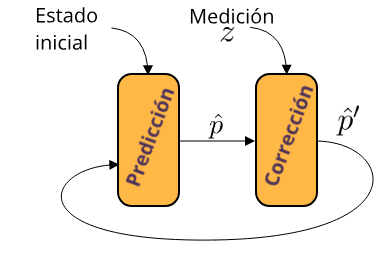
\includegraphics[width=0.5\textwidth]{figures/filtro_kalman.png}
\caption{Ciclo predicción-corrección del filtro de Kalman, repetido en cada frame para cada objeto seguido.}
\label{fig:fases-filtro-kalman}
\end{figure}

Este ciclo tiene una consecuencia práctica importante para el tracking: aun
cuando un objeto deja de detectarse durante varios frames (por ejemplo, por
una oclusión), el filtro de Kalman sigue pudiendo predecir su posición
probable basándose en su movimiento anterior, lo que permite mantener viva
su identidad y recuperar la asociación correcta cuando vuelve a detectarse.
Los tres algoritmos comparados y considerados en este proyecto (SORT,
OC-SORT y ByteTrack, sección~\ref{sec:fundamentos-algoritmos}) usan
variantes de un filtro de Kalman como modelo de movimiento subyacente.

\subsection{Solapamiento entre cajas: IoU}
\label{subsec:fundamentos-iou}

Para decidir si una detección de un frame corresponde al mismo objeto que
una predicción de Kalman (o que otra detección de un frame anterior), los
métodos de \emph{tracking-by-detection} necesitan una medida de similitud
entre dos cajas delimitadoras. La más utilizada, por su simplicidad y bajo
coste computacional, es la \textbf{Intersección sobre Unión} (\emph{Intersection
over Union}, IoU): dadas dos cajas $A$ y $B$, se define como

\begin{equation}
\mathrm{IoU}(A, B) = \frac{|A \cap B|}{|A \cup B|},
\label{eq:fundamentos-iou}
\end{equation}

es decir, el área de la región donde ambas cajas se solapan, dividida entre
el área total que cubren entre las dos. La IoU vale 1 cuando las cajas
coinciden exactamente y 0 cuando no se solapan en absoluto, lo que la hace
directamente interpretable como un porcentaje de acuerdo espacial (véase la
Figura~\ref{fig:fundamentos-iou}).

\begin{figure}[htp]
\centering
\begin{tikzpicture}[scale=0.9]
\draw[fill=blue!15, draw=blue!70, thick] (0,0) rectangle (3.2,2.4);
\node[blue!70] at (0.4,2.7) {\footnotesize Caja $A$ (predicción)};
\draw[fill=orange!20, draw=orange!80, thick, fill opacity=0.6] (1.6,0.8) rectangle (4.6,3.0);
\node[orange!80!black] at (4.6,3.3) {\footnotesize Caja $B$ (detección)};
\node[font=\footnotesize] at (2.3,1.5) {$A \cap B$};
\end{tikzpicture}
\caption{Intersección sobre Unión (IoU) entre una caja predicha por Kalman
(A) y una detección real (B): la región sombreada de solape, dividida entre
el área total ocupada por ambas cajas.}
\label{fig:fundamentos-iou}
\end{figure}

\subsection{El problema de asignación y el algoritmo húngaro}
\label{subsec:fundamentos-hungaro}

Una vez calculada una matriz de similitud (por ejemplo, de IoU) entre todas
las predicciones activas y todas las detecciones de un frame, queda por
resolver el \textbf{problema de asignación}: encontrar la correspondencia
uno a uno entre predicciones y detecciones que maximice la similitud total,
sin que ninguna detección se asocie a más de una predicción ni viceversa.
Resolver este problema por fuerza bruta (probar todas las combinaciones
posibles) tiene un coste factorial en el número de objetos, inviable ya
con unas pocas decenas de jugadores en pantalla.

El \textbf{algoritmo húngaro} \citep{wikipedia2026hungaro} resuelve este
problema de forma exacta y en tiempo polinómico. Dada una matriz de coste
$M$ (que puede construirse, por ejemplo, como $1 - \mathrm{IoU}$, de modo
que minimizar coste equivale a maximizar solapamiento), el algoritmo
encuentra la asignación completa de coste mínimo mediante una serie de
transformaciones de la matriz que no alteran la asignación óptima pero
reducen progresivamente el problema, hasta poder leer la solución
directamente. En la práctica, ninguno de los algoritmos de tracking usados
en este proyecto implementa el algoritmo húngaro desde cero: todos delegan
en la implementación ya optimizada de \texttt{scipy} o de librerías
equivalentes, a través de la librería \texttt{boxmot} descrita en la
sección~\ref{sec:implementacion-entorno}.

Un detalle que puede ser importante a la hora de entender ByteTrack en la
sección~\ref{subsec:fundamentos-bytetrack} es que no toda asignación con
coste finito se acepta: se suele imponer un umbral mínimo de similitud
(por ejemplo, IoU mínima) por debajo del cual una predicción y una detección no
se consideran candidatas a asociarse, aunque el algoritmo húngaro las
hubiera emparejado matemáticamente. Las predicciones que no encuentran
ninguna detección compatible se marcan como no observadas en ese frame
, mientras que las
detecciones que no encuentran ninguna predicción compatible inician una
identidad nueva.

\section{Algoritmos de tracking comparados}
\label{sec:fundamentos-algoritmos}

Con los fundamentos de las secciones anteriores, esta sección describe los
dos algoritmos efectivamente implementados y comparados en este proyecto
ByteTrack y OC-SORT así como el algoritmo histórico del que ambos
derivan (SORT) y las familias de algoritmos que se consideraron pero
finalmente no se implementaron, con la justificación de por qué.

\subsection{SORT: el punto de partida}
\label{subsec:fundamentos-sort}

\textbf{SORT} (\emph{Simple Online and Realtime Tracking},
\citealp{bewley2016sort, ultralytics2026trackingtools}) es el algoritmo que sentó las bases del
\emph{tracking-by-detection} moderno: para cada objeto seguido, mantiene un
filtro de Kalman (sección~\ref{subsec:fundamentos-kalman}) que predice su
posición en el frame actual; calcula la IoU (sección~\ref{subsec:fundamentos-iou})
entre esas predicciones y todas las detecciones del frame; resuelve la
asignación óptima con el algoritmo húngaro
(sección~\ref{subsec:fundamentos-hungaro}); y actualiza cada filtro de
Kalman con la detección que le ha correspondido. Su principal virtud, que
explica su influencia posterior, es la simplicidad: no requiere ningún
modelo de apariencia visual ni entrenamiento adicional más allá del propio
detector de objetos, lo que lo hace extremadamente rápido.

SORT tiene, sin embargo, una limitación conocida que motivó buena parte de
las mejoras posteriores: solo considera para la asociación las detecciones
de \emph{alta confianza} del detector, descartando directamente las de
confianza intermedia o baja. En escenarios con oclusiones frecuentes como
el fútbol, un jugador parcialmente ocluido suele generar una detección de
confianza más baja (o directamente no generar ninguna), lo que provoca que
SORT pierda su identidad con más facilidad de la deseable y genere más
\emph{cambios de identidad} (\emph{ID switches}) de los necesarios. Esta
limitación es precisamente la que aborda ByteTrack.

En \texttt{boxmot}, la librería usada en este proyecto
(sección~\ref{sec:implementacion-entorno}), no existe una implementación
del SORT original independiente: la clase disponible más próxima es
\texttt{OCSORT}, su evolución directa descrita en la
sección~\ref{subsec:fundamentos-ocsort}. Por ese motivo, y como se explica
en el capítulo~\ref{cap:implementacion}, el script de este proyecto que
originalmente pretendía implementar SORT (\texttt{sort\_alg.py}) contiene en
realidad OC-SORT, quedando el nombre del fichero como huella de
esa decisión.

\subsection{OC-SORT: SORT centrado en la observación}
\label{subsec:fundamentos-ocsort}

\textbf{OC-SORT} (\emph{Observation-Centric SORT}, \citealp{cao2023ocsort})
identifica y corrige dos problemas concretos de SORT, sin abandonar su
simplicidad y velocidad. El primero es lo que sus autores llaman
\emph{acumulación de error durante la desaparición}: cuando un objeto deja
de detectarse durante varios frames (oclusión), el filtro de Kalman de
SORT sigue extrapolando su posición usando exclusivamente su propio modelo
de movimiento, sin ninguna corrección, de modo que el error de la
predicción crece sin control cuanto más dura la oclusión; al reaparecer el
objeto, la predicción puede estar ya demasiado lejos de la posición real
para una asociación correcta. El segundo es la sensibilidad del filtro de
Kalman a los movimientos no lineales,
especialmente marcados en fútbol.

OC-SORT resuelve ambos problemas centrando el filtro en las
\emph{observaciones reales} en lugar de en el estado interno acumulado por
Kalman: en lugar de corregir el filtro paso a paso con predicciones
intermedias durante toda la desaparición, cuando el objeto reaparece
OC-SORT recalcula directamente su trayectoria a partir de la última
observación real conocida antes de desaparecer y la primera observación
real al reaparecer, evitando así la deriva acumulada. Este enfoque, más
robusto ante oclusiones largas y movimientos bruscos, es el que motivó su
inclusión en la comparativa de este proyecto junto con ByteTrack.

\subsection{ByteTrack: aprovechar todas las detecciones}
\label{subsec:fundamentos-bytetrack}

\textbf{ByteTrack} \citep{zhang2022bytetrack, ultralytics2026trackingtools} aborda directamente la
limitación de SORT descrita en la sección~\ref{subsec:fundamentos-sort}: en
lugar de descartar las detecciones de baja confianza, las aprovecha en una
\emph{segunda ronda} de asociación. Su procedimiento, para cada frame, es
el siguiente:

\begin{enumerate}
  \item Se separan las detecciones del frame en dos grupos según un umbral
        de confianza: de \textbf{alta} y de \textbf{baja} confianza.
  \item \textbf{Primera asociación}: se emparejan las predicciones de
        Kalman con las detecciones de alta confianza, con el procedimiento
        estándar de IoU y algoritmo húngaro
        (secciones~\ref{subsec:fundamentos-iou}
        y~\ref{subsec:fundamentos-hungaro}).
  \item \textbf{Segunda asociación}: las predicciones que no encontraron
        pareja en el paso anterior normalmente son objetos parcialmente
        ocluidos cuya detección, si existe, es de baja confianza. Estas
        predicciones se intentan emparejar de nuevo, esta vez únicamente contra las
        detecciones de baja confianza.
  \item Las predicciones que siguen sin pareja tras ambas rondas se
        mantienen como activas sin observación (apoyándose en el filtro de
        Kalman) durante un número limitado de frames antes de eliminarse
        definitivamente y las detecciones de alta confianza que no
        encontraron ninguna predicción compatible inician identidades
        nuevas.
\end{enumerate}

\begin{figure}[htp]
\centering
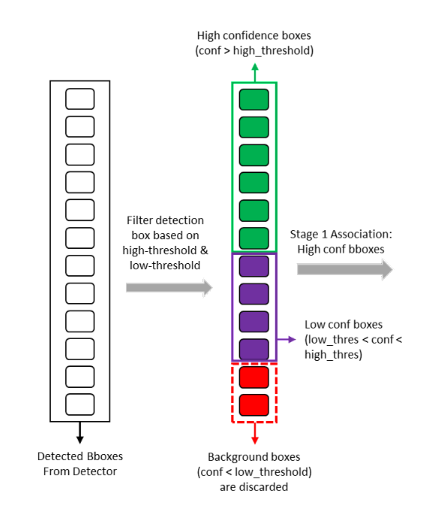
\includegraphics[width=0.7\textwidth]{figures/bytetrack-detec.png}
\caption{Las dos rondas de asociación de ByteTrack: primero con
detecciones de alta confianza, después con las de baja confianza,
recuperando así objetos parcialmente ocluidos que SORT descartaría
\citep{zhang2022bytetrack}.}
\label{fig:fundamentos-bytetrack}
\end{figure}

Esta segunda ronda es, precisamente, lo que hace a ByteTrack especialmente
adecuado para el fútbol: un jugador ocluido detrás de otro suele seguir
generando una detección débil (de baja confianza) en lugar de ninguna
detección, y ByteTrack es capaz de aprovechar esa señal parcial en lugar de
descartarla, a diferencia de SORT y, en menor medida, de OC-SORT.

\subsection{Trackers con re-identificación visual: considerados y no implementados}
\label{subsec:fundamentos-reid}

Los tres algoritmos descritos hasta ahora (SORT, OC-SORT, ByteTrack)
pertenecen a la familia de trackers \emph{sin apariencia}: solo usan la
posición y el tamaño de las cajas delimitadoras para asociar, nunca el
aspecto visual del objeto. Existe una familia paralela de algoritmos que
incorpora, además, un modelo de \textbf{re-identificación} (\emph{Re-ID}):
una red neuronal, entrenada por separado, que extrae un vector numérico
(\emph{embedding}) representativo de la apariencia visual de cada objeto,
de modo que dos detecciones del mismo objeto puedan reconocerse por similitud de
apariencia y no solo por proximidad espacial. \textbf{DeepSORT}
\citep{wojke2017deepsort, ultralytics2026trackingtools} fue el primer algoritmo relevante en incorporar
esta idea sobre la base de SORT, y su enfoque se ha extendido después a
variantes más recientes como StrongSORT o BoT-SORT, todas ellas también
disponibles en \texttt{boxmot}.

El tutor de este proyecto planteó explícitamente, en una de las reuniones
de seguimiento (sección~\ref{sec:gestion-roles}), la posibilidad de ampliar
la comparativa con algoritmos de esta familia. Finalmente no se ha
incorporado ningún tracker con Re-ID a este proyecto, por dos motivos
principales. En primer lugar, una comparación justa exigiría fijar el mismo
modelo de Re-ID para todos los algoritmos comparados (por ejemplo,
\texttt{osnet\_x0\_25\_msmt17}, disponible directamente en
\texttt{boxmot}), lo que añade una variable más --la calidad del propio
modelo de Re-ID, no entrenado por el equipo del proyecto ni específico de
fútbol-- a una comparativa que, sin esa variable, ya resultaba
suficientemente rica con el estudio de hiperparámetros de los dos
algoritmos sin apariencia (capítulo~\ref{cap:implementacion}). En segundo
lugar, como se ha señalado en la sección~\ref{sec:fundamentos-mot}, la
apariencia visual es un criterio especialmente poco discriminativo en
fútbol (los compañeros de equipo visten de forma prácticamente idéntica),
lo que hace previsible que el margen de mejora aportado por Re-ID en este
dominio concreto sea menor que en otros escenarios de MOT donde cada
persona viste de forma distinta.

\section{Métricas de evaluación de sistemas de tracking}
\label{sec:fundamentos-metricas}

Comparar dos algoritmos de tracking exige una forma objetiva de medir su
rendimiento sobre el \emph{ground truth} (\texttt{gt.txt},
sección~\ref{subsec:fundamentos-soccernet-tracking}). Esta sección presenta
las tres familias de métricas empleadas en este proyecto y calculadas con
\texttt{TrackEval} (sección~\ref{sec:implementacion-evaluacion}): MOTA/MOTP
(las más clásicas), IDF1 (centrada en la consistencia de identidad) y HOTA
(la más reciente y equilibrada, adoptada como métrica principal de este
proyecto).

\subsection{CLEAR MOT: MOTA y MOTP}

Las métricas \textbf{CLEAR MOT} \citep{bernardin2008clearmot} fueron,
durante más de una década, el estándar de facto en la evaluación de
sistemas de tracking. \textbf{MOTA} (\emph{Multiple Object Tracking
Accuracy}) resume en un único porcentaje tres tipos de error acumulados a
lo largo de toda la secuencia: falsos negativos (objetos reales no
detectados), falsos positivos (detecciones que no corresponden a ningún
objeto real) y cambios de identidad (\emph{ID switches}, cuando el
algoritmo confunde la identidad de un objeto con la de otro). \textbf{MOTP}
(\emph{Multiple Object Tracking Precision}), complementaria a MOTA, mide la
precisión espacial media de las cajas correctamente emparejadas (cuánto se
solapan, en promedio, con el \emph{ground truth}), sin penalizar los
errores de asociación que ya recoge MOTA.

La principal limitación de MOTA, señalada posteriormente varias veces
en este documento \citep{luiten2021hota}, es que pondera con mucho más peso los
errores de detección (falsos positivos y negativos) que los errores de
asociación (cambios de identidad): un algoritmo puede detectar
correctamente a casi todos los jugadores en casi todos los frames y aun así
confundir sistemáticamente sus identidades, obteniendo una MOTA
engañosamente alta pese a ser, en la práctica, poco útil para cualquier
análisis que dependa de trayectorias individuales consistentes, como el
pipeline de metadatos de este mismo proyecto
(sección~\ref{sec:implementacion-metadatos}).

\subsection{IDF1}

\textbf{IDF1} \citep{ristani2016idf1} nace precisamente para corregir ese
desequilibrio, centrando la evaluación en la consistencia de identidad en
lugar de en la detección frame a frame. Se calcula como la media armónica
(F1) entre la precisión y la exhaustividad (\emph{recall}) de identidad,
calculadas tras resolver una única asignación óptima,de nuevo mediante el
algoritmo húngaro, sección~\ref{subsec:fundamentos-hungaro} entre las
trayectorias predichas por el algoritmo y las trayectorias reales del
\emph{ground truth} a lo largo de \emph{toda} la secuencia, no frame a
frame. En la práctica, IDF1 penaliza con mucha más severidad que MOTA los
cambios de identidad, y es una de las tres métricas reportadas en los
resultados de este proyecto (capítulo~\ref{cap:pruebas}).

\subsection{HOTA: la métrica principal de este proyecto}
\label{subsec:fundamentos-hota}

\textbf{HOTA} (\emph{Higher Order Tracking Accuracy},
\citealp{luiten2021hota, luiten2021hotablog}) es la métrica más reciente de las tres, propuesta
explícitamente para resolver el desequilibrio entre detección y asociación
que arrastraban tanto MOTA (sesgada hacia la detección) como IDF1 (sesgada
hacia la asociación). HOTA se define como la media geométrica de dos
componentes independientes:

\begin{equation}
\mathrm{HOTA} = \sqrt{\mathrm{DetA} \times \mathrm{AssA}},
\label{eq:fundamentos-hota}
\end{equation}

donde \textbf{DetA} (\emph{Detection Accuracy}) mide, de forma análoga a
MOTA, qué tan bien se detectan los objetos, y \textbf{AssA}
(\emph{Association Accuracy}) mide, de forma análoga a IDF1, qué tan bien
se mantienen las identidades a lo largo del tiempo. Al tomar la media
geométrica en lugar de una suma ponderada, HOTA exige que un algoritmo sea
bueno en ambos aspectos simultáneamente: un valor muy alto en uno de
los dos componentes no puede compensar un valor muy bajo en el otro, a
diferencia de lo que ocurriría con una media aritmética.

Una particularidad adicional de HOTA, relevante para la interpretación de
los resultados de este proyecto (capítulo~\ref{cap:pruebas}), es que ambos
componentes se calculan y promedian sobre un rango de umbrales de
solapamiento IoU, en lugar
de sobre un único umbral fijo como hacen MOTA e IDF1, que en TrackEval,
se calculan típicamente al 50\,\%
de IoU. Esta característica hace de HOTA una métrica más exigente y
completa, ya que resume el comportamiento del algoritmo tanto ante
exigencias de solapamiento laxas como estrictas, y es la razón por la que
se ha adoptado como métrica principal de comparación en este proyecto.

\section{Detección del balón}
\label{subsec:fundamentos-balon}

Aunque, como se ha explicado en la sección~\ref{sec:fundamentos-mot}, este
proyecto no aborda la detección de objetos (se parte de \texttt{det.txt}
ya calculado), existe un matiz importante: SoccerNet-Tracking incluye en
ese mismo fichero las detecciones del balón mezcladas con las de jugadores
y árbitros, sin distinguir explícitamente de qué tipo de objeto se trata
cada detección. Separar el balón del resto de objetos es, por tanto, un
paso de preprocesamiento necesario antes de aplicar cualquier algoritmo de
tracking, ya que el balón sigue una dinámica de movimiento completamente
distinta a la de una persona, es más rápido y con rebotes. Por tanto,
no tiene sentido
tratarlo con el mismo filtro de Kalman ni contarlo en las métricas de
tracking de personas.

La primera aproximación explorada para resolver este paso fue emplear un
detector de objetos entrenado con aprendizaje profundo, concretamente
\textbf{YOLO} (\emph{You Only Look Once}, \citealp{redmon2016yolo, ultralytics2026yolov8}) en su
versión ligera YOLOv8n, aplicado directamente sobre los frames para
localizar el balón de forma independiente al \texttt{det.txt} del dataset.
Este enfoque se descartó tras las primeras pruebas: el modelo, sin
reentrenar específicamente para balones de fútbol en las condiciones de
cámara e iluminación de las retransmisiones de SoccerNet, obtenía
resultados muy pobres, tanto falsos negativos (balón no detectado) como
falsos positivos sobre otros objetos redondeados y claros del campo, y
entrenarlo específicamente para esta única tarea auxiliar quedaba fuera del
alcance proporcional de este proyecto.

Se optó, en su lugar, por un \textbf{filtro geométrico} simple aplicado
directamente sobre las detecciones ya existentes en \texttt{det.txt}: una
detección se clasifica como balón si su área en píxeles es menor que un
umbral y su proporción ancho/alto es próxima a 1 (es decir, aproximadamente
cuadrada, coherente con la silueta de un balón visto desde prácticamente
cualquier ángulo), condiciones que rara vez cumple una persona. Este
filtro, con los umbrales exactos empleados, se detalla en la
sección~\ref{sec:implementacion-tracking} del
capítulo~\ref{cap:implementacion}; se trata de una heurística simple y con
limitaciones conocidas (puede confundir a un jugador muy lejano y pequeño
con el balón), pero suficiente para el propósito de excluir al balón del
tracking de personas sin necesidad de entrenar un modelo adicional.

\section{Clasificación no supervisada de jugadores por equipo: K-means y el árbitro}
\label{sec:fundamentos-kmeans}

Una vez obtenidas las trayectorias de los jugadores (capítulo~\ref{cap:implementacion}),
buena parte de los metadatos deportivos de interés como mapas de calor por
equipo, posesión por equipo (sección~\ref{sec:implementacion-metadatos})
requieren saber a qué equipo pertenece cada jugador. SoccerNet-Tracking no
proporciona esa información directamente, por lo que este proyecto la
infiere a partir del color dominante de la camiseta de cada jugador,
mediante \textbf{K-means}.

K-means \citep{ibm2026kmeans} es un algoritmo de \textbf{aprendizaje no
supervisado}: a diferencia de los algoritmos de aprendizaje supervisado que
aprenden a partir de ejemplos ya etiquetados con la respuesta correcta
(sección~\ref{sec:fundamentos-ia}), K-means agrupa datos sin ninguna
etiqueta previa, únicamente a partir de su similitud mutua. Dado un
conjunto de puntos (en este proyecto, colores representados como vectores
de tres componentes en el espacio BGR) y un número $k$ de grupos deseado,
el algoritmo procede de forma iterativa:

\begin{enumerate}
  \item Se inicializan $k$ centroides (puntos representativos de cada
        grupo), habitualmente de forma aleatoria o mediante alguna
        heurística de inicialización.
  \item \textbf{Asignación}: cada punto del conjunto de datos se asigna al
        centroide más cercano (típicamente, en distancia euclídea).
  \item \textbf{Actualización}: cada centroide se recalcula como la media
        de todos los puntos que se le han asignado.
  \item Los pasos 2 y 3 se repiten hasta que las asignaciones dejan de
        cambiar (convergencia) o se alcanza un número máximo de
        iteraciones.
\end{enumerate}

\begin{figure}[htp]
\centering
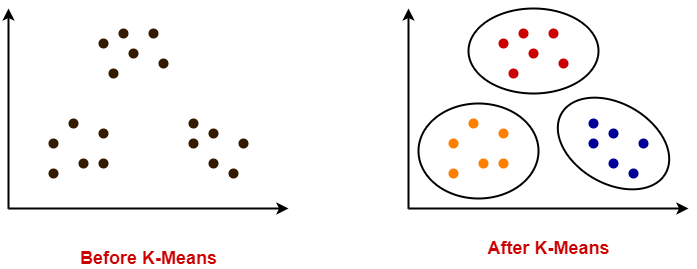
\includegraphics[width=0.85\textwidth]{figures/kmeans_before_after.png}
\caption{Efecto de K-means sobre un conjunto de puntos: antes del
agrupamiento (izquierda) y después de converger a $k=3$ grupos, cada uno
alrededor de su centroide (derecha) \citep{gatevidyalay2026kmeans}.}
\label{fig:fundamentos-kmeans-ejemplo}
\end{figure}

Formalmente, lo que este procedimiento iterativo minimiza es la suma de
las distancias euclídeas al cuadrado entre cada punto y el centroide de su
grupo \citep{ibm2026kmeans}:

\begin{equation}
\arg\min_{S} \sum_{i=1}^{k} \sum_{\mathbf{x} \in S_i} \lVert \mathbf{x} - \boldsymbol{\mu}_i \rVert^2,
\label{eq:fundamentos-kmeans}
\end{equation}

donde $S_i$ es el conjunto de puntos asignados al grupo $i$-ésimo y
$\boldsymbol{\mu}_i$ su centroide. El paso de \textbf{actualización} de
cada centroide como la media de sus puntos asignados es, precisamente, el
que reduce este error en cada iteración, hasta alcanzar un mínimo local.

En este proyecto, K-means se aplica en dos niveles, detallados con sus
parámetros concretos en la sección~\ref{sec:implementacion-metadatos}: primero,
con $k=1$, para extraer el color dominante de la camiseta de cada
detección individual de jugador (el color medio de una región recortada del
torso); después, con $k=2$ sobre el conjunto de todos esos colores
dominantes, asumiendo que existen exactamente dos equipos con colores de
camiseta distintos entre sí.

Esa asunción de $k=2$ es, precisamente, la limitación más relevante de este
enfoque y una de las cosas consideradas pero no resueltas en este proyecto:
el árbitro, con una camiseta de color distinto a la de ambos equipos, no
encaja en ninguno de los dos grupos y termina asignado por K-means al
centroide más próximo por color, es decir, a uno de los dos equipos de
forma incorrecta. Se valoró pero no se llegó a implementar una variante con
$k=3$ combinada con una heurística adicional (el grupo con menos
detecciones totales, dado que solo hay un árbitro principal frente a unos
once jugadores por equipo, se etiquetaría como árbitro en lugar de como
tercer equipo); esta mejora queda documentada como línea de trabajo futuro
en el capítulo~\ref{cap:conclusiones}.

\section{Homografía y proyección de coordenadas}
\label{sec:fundamentos-homografia}

Las posiciones de los jugadores que produce el tracking están expresadas en
\textbf{coordenadas de píxel} de la imagen de la cámara de retransmisión:
un sistema de referencia bidimensional propio de cada frame, sin relación
directa con las distancias reales sobre el terreno de juego. Para poder
calcular metadatos con sentido físico (distancia recorrida en metros,
velocidad en km/h, o simplemente representar las posiciones sobre un dibujo
del campo con proporciones correctas (sección~\ref{sec:implementacion-metadatos}))
es necesario transformar esas coordenadas de píxel a
\textbf{coordenadas reales del campo}, expresadas en metros sobre un plano
cenital.

\begin{figure}[htp]
\centering
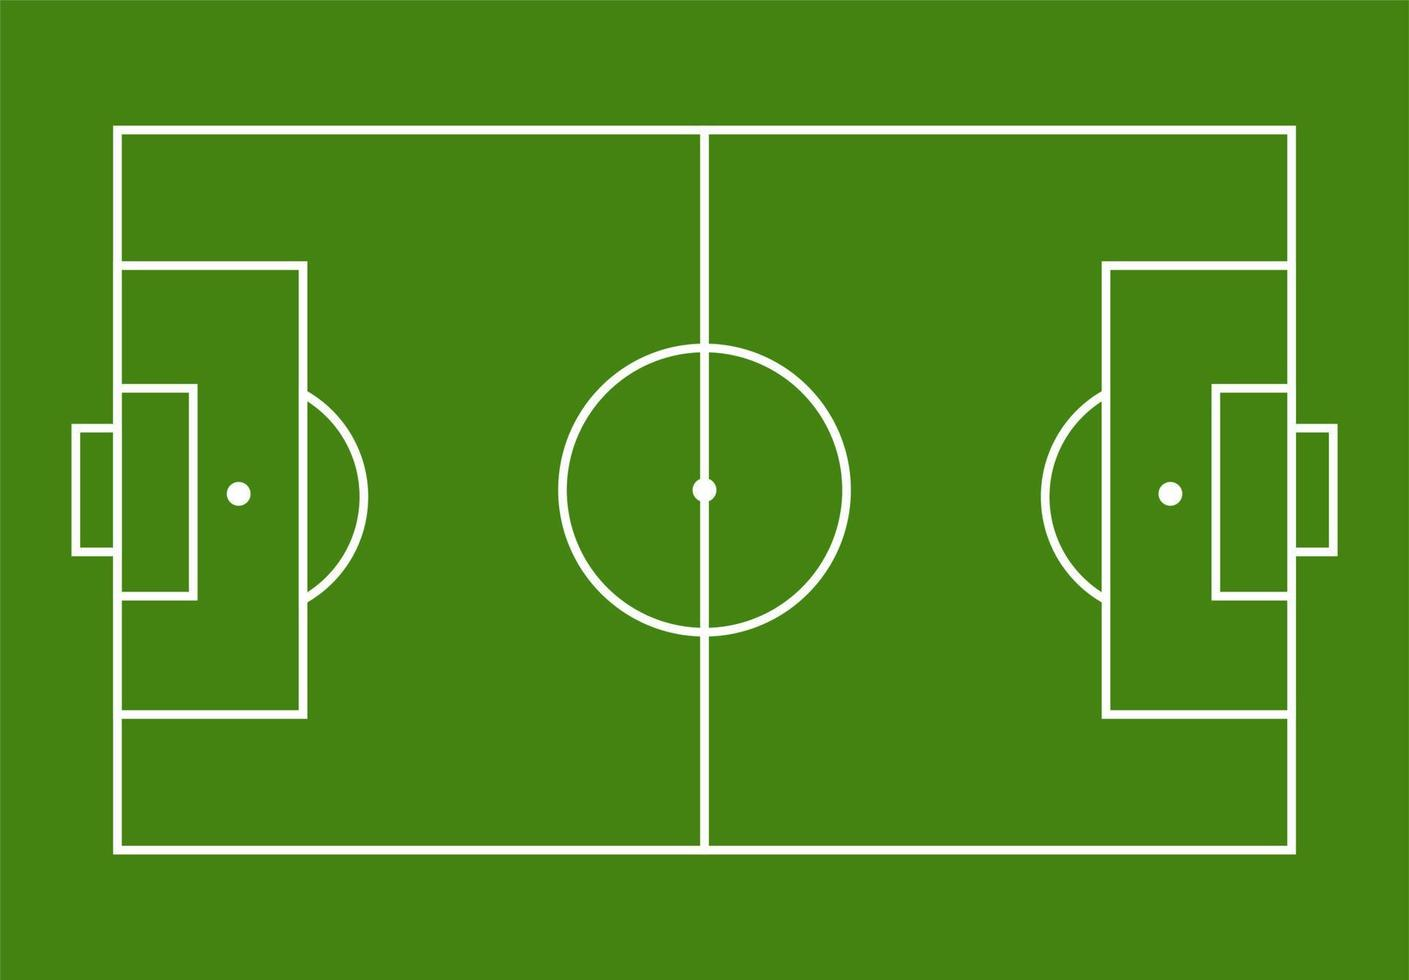
\includegraphics[width=0.75\textwidth]{figures/campo_futbol_vecteezy.jpg}
\caption{Campo de fútbol estándar visto en planta \citep{vecteezy2026campo}. Las
medidas FIFA reglamentarias empleadas como referencia para la homografía y
para los mapas de calor de este proyecto
(sección~\ref{sec:implementacion-metadatos}) son: 105\,m $\times$ 68\,m de
terreno de juego, área grande 16{,}5\,m $\times$ 40{,}3\,m, área pequeña
5{,}5\,m $\times$ 18{,}3\,m, círculo central de 9{,}15\,m de radio.}
\label{fig:fundamentos-campo}
\end{figure}

Esa transformación, cuando la cámara se puede aproximar como una
proyección perspectiva pura sobre un plano. El terreno de juego es, a
efectos prácticos, plano, se describe matemáticamente mediante una
\textbf{homografía}: una matriz $H$ de $3\times 3$ que relaciona las
coordenadas homogéneas de un punto en el plano imagen,
$\mathbf{p} = (x, y, 1)^\top$, con las coordenadas homogéneas del punto
correspondiente en el plano del campo, $\mathbf{p}' = (x', y', 1)^\top$,
mediante

\begin{equation}
\mathbf{p}' \sim H\,\mathbf{p},
\label{eq:fundamentos-homografia}
\end{equation}

donde $\sim$ indica igualdad salvo un factor de escala, propio de las
coordenadas homogéneas \citep{opencv2026homography}. La matriz $H$ tiene 8
grados de libertad (9 elementos menos 1 por el factor de escala libre), por
lo que puede calcularse de forma exacta a partir de 4 pares de puntos
correspondientes conocidos (un punto en la imagen y su posición real
equivalente en el campo) mediante un sistema de ecuaciones lineales;
disponer de más de 4 correspondencias permite, además, calcular $H$ por
mínimos cuadrados y obtener una estimación más robusta frente a errores de
medición en los puntos de referencia.

\begin{figure}[htp]
\centering
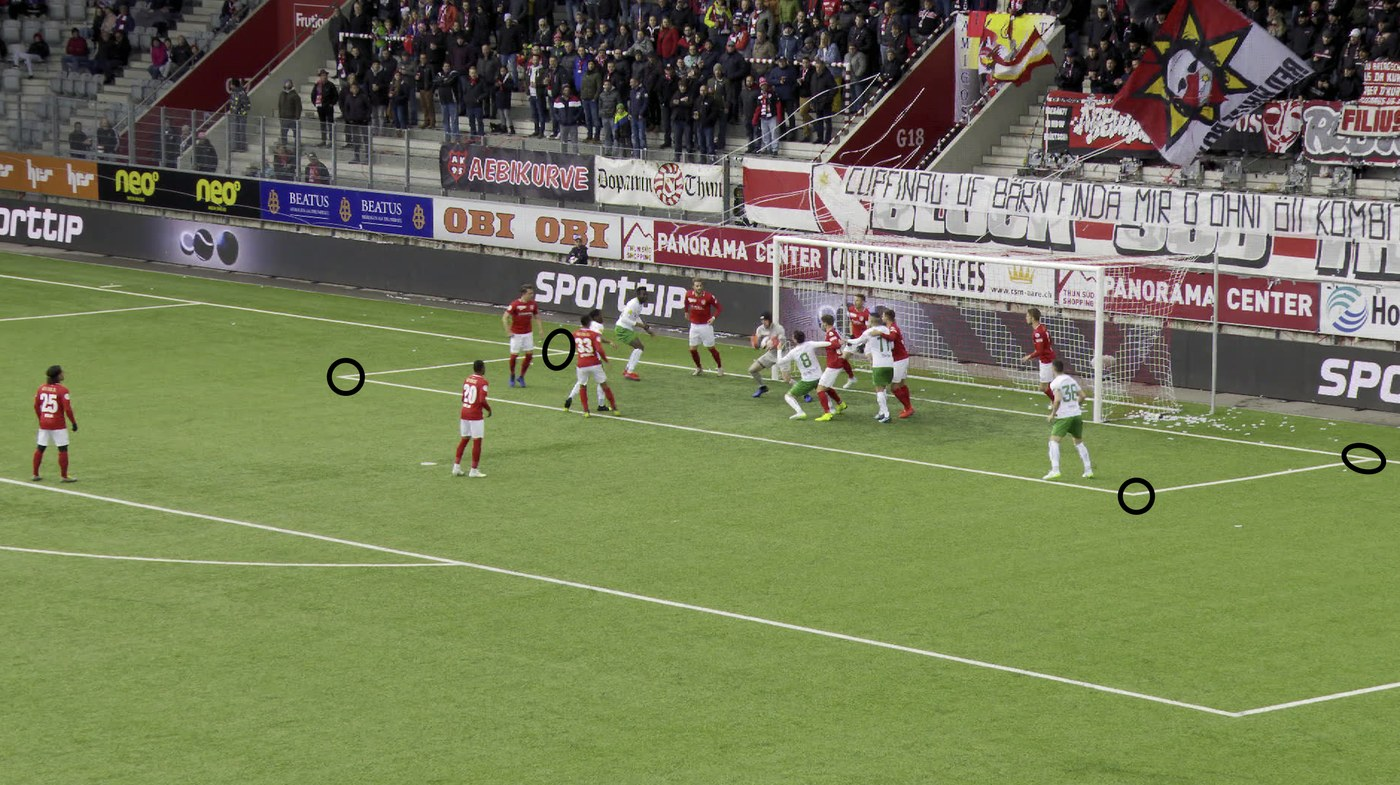
\includegraphics[width=0.92\textwidth]{figures/homografia-real.jpg}
\caption{Puntos de referencia marcados sobre un frame real de
retransmisión, usados para calcular la homografía: las cuatro esquinas
del área pequeña, cuyas coordenadas de campo son conocidas por las
medidas FIFA (Figura~\ref{fig:fundamentos-campo}).}
\label{fig:fundamentos-homografia-ejemplo}
\end{figure}

En un escenario ideal, en el que la cámara de retransmisión permaneciera
completamente fija durante todo el partido, bastaría con calcular $H$ una
única vez, identificando manualmente 4 puntos de referencia reconocibles en
el campo, por ejemplo, las esquinas del área pequeña, cuyas medidas FIFA
son conocidas y fijas (5{,}5\,m $\times$ 18{,}3\,m,
Figura~\ref{fig:fundamentos-campo}) y sus coordenadas de píxel
correspondientes en un frame representativo. Esta es, de hecho, la
aproximación seguida en este proyecto, pero limitada deliberadamente a
tramos concretos de vídeo con cámara estable, dado que las cámaras de
retransmisión real de SoccerNet se mueven de forma continua (paneos,
zooms) a lo largo de toda la secuencia (lo que exigiría recalcular $H$
de forma dinámica, frame a frame, un problema de calibración de cámara
considerablemente más complejo y fuera del alcance de este proyecto). Las
implicaciones prácticas de esta limitación, y la alternativa de proyección
aproximada empleada para el resto del dataset, se detallan en la
sección~\ref{sec:implementacion-homografia}.

\section{Trabajos relacionados y posicionamiento de este TFG}
\label{sec:fundamentos-relacionados}

El propio ecosistema SoccerNet organiza, además del dataset, un reto anual
de seguimiento multiobjeto (\emph{SoccerNet Player Tracking Challenge}) con
un servidor de evaluación público y un \emph{leaderboard} de equipos
participantes, lo que ofrece el punto de comparación más directo y
verificable para situar los resultados de este proyecto frente al estado
del arte práctico.

La edición 2023 del reto \citep{cioppa2023soccernetchallenges}, con 7 equipos
y 83 envíos, resulta muy informativa sobre qué enfoques resultan
competitivos en la práctica: el equipo ganador (Kalisteo) alcanzó
HOTA\,=\,75{,}61 combinando un detector YOLO-X afinado con un tracker
propio basado en el algoritmo húngaro
y un filtro de Kalman con compensación de movimiento de cámara; y, de forma especialmente
relevante para las decisiones de este proyecto, varios de los equipos
mejor clasificados construyeron su solución precisamente sobre
\textbf{ByteTrack} o la familia \textbf{SORT/OC-SORT}, por ejemplo, SAIVA Tracking
sobre ByteTrack, ZTrackers sobre YOLOv5 combinado con ByteTrack, y
MOT4MOT sobre DeepOCSORT, lo que confirma que ambos algoritmos
constituyen una base representativa y competitiva del estado del arte
práctico.

El HOTA integrado en test obtenido en este proyecto
con OC-SORT (75{,}43), resulta muy próximo al del equipo ganador del
reto oficial 2023 (75{,}61) aunque a partir de una posición menos favorable
en dos aspectos: sin ningún entrenamiento ni ajuste de detector
específico para fútbol, y con los algoritmos de tracking en su
configuración por defecto para esa comparación concreta. No se trata, por
tanto, de una comparación totalmente equivalente ni se trata de un intento
de superar el estado del arte del reto, es una referencia
que sitúa los resultados de este TFG en un rango realista y defendible
frente a soluciones desarrolladas específicamente para competir.

Este proyecto no busca competir en ese \emph{leaderboard}, sino dos objetivos distintos que
el reto no cubre: una comparación rigurosa entre dos algoritmos clásicos de
\emph{tracking-by-detection} bajo las mismas condiciones mi. Y segundo, la construcción de un pipeline
completo de extracción de metadatos deportivos y la
exposición des sus resultados en una aplicación web, que va
más allá de la propia tarea de tracking en la que se detiene el reto
oficial.


    \chapter{Gestión del proyecto}
\label{cap:gestion}

Todo proyecto de ingeniería del software requiere, además de la resolución
técnica del problema planteado, una gestión del propio proceso de
trabajo: qué metodología se sigue, cómo se reparte el esfuerzo en el tiempo,
qué recursos se necesitan y qué riesgos pueden comprometer el resultado
final. Este capítulo documenta esa gestión para el presente proyecto: la
metodología de trabajo adoptada, las fases en que se ha dividido el
desarrollo, los roles ejercidos, la planificación temporal (inicial y
revisada), la estimación de recursos y presupuesto, y los planes de gestión
de riesgos y de calidad aplicados.

\section{Metodología de trabajo}
\label{sec:gestion-metodologia}

Este proyecto se ha desarrollado siguiendo un enfoque iterativo e
incremental, guiado por instrucciones de seguimiento con el tutor.
En lugar de fijar de antemano una especificación cerrada de todo el sistema
, cada bloque de trabajo se ha
planteado como una iteración corta que produce un resultado funcional y
evaluable, cuyas conclusiones determinan el siguiente paso. Este enfoque es
especialmente adecuado en un proyecto como este,
en el que algunas decisiones como qué algoritmos comparar, qué metadatos
extraer, hasta dónde llevar la calibración de cámara dependían de
resultados intermedios que no podían conocerse de antemano: no tenía
sentido, por ejemplo, comprometerse a un pipeline completo de metadatos
antes de comprobar que la comparativa de algoritmos de tracking daba
resultados sólidos y defendibles.

Dentro de ese marco iterativo, cada ciclo de trabajo ha seguido
aproximadamente la misma secuencia: (1) plantear una pregunta concreta o un
objetivo acotado a partir de las conclusiones del ciclo anterior y, en las
ideas claves de las instrucciones del tutor; (2) implementar la
solución mínima que permita responder a esa pregunta; (3) evaluar el
resultado con datos reales, normalmente mediante las métricas MOT estándar
descritas en el capítulo~\ref{cap:fundamentos}; y (4) plantear la idea y 
decisiones tomadas al tutor y documentar la decisión
tomada (incluida la opción de descartar el enfoque probado) antes de
pasar al siguiente ciclo. Este último punto ha sido determinante para la
redacción de esta memoria: al quedar registrada la razón de cada decisión
en el momento en que se tomó, ha sido posible construir la memoria de forma
detallada, incluyendo no solo los resultados finales, sino también el proceso seguido para llegar hasta ellos.

El seguimiento del trabajo entre reuniones se ha apoyado en un documento de
anotaciones propio, actualizado de forma continua, donde se registran
decisiones tomadas, resultados numéricos, problemas de entorno encontrados
y su solución, e ideas evaluadas y descartadas. Este documento ha sido la fuente principal para poder
documentar todo el proceso de desarrollo en esta memoria.

\section{Fases del proyecto}
\label{sec:gestion-fases}

Sobre la metodología iterativa descrita, el trabajo se ha organizado en
siete fases principales, que se recorrieron de forma mayoritariamente
secuencial pero con solapamientos puntuales entre fases adyacentes; en
particular entre la fase 4 (estudio de hiperparámetros) y la fase 5
(pipeline de metadatos), ya que la configuración óptima de cada algoritmo
se fue consolidando mientras ya se trabajaba en los primeros metadatos, y
entre la fase 5 y la fase 7 (redacción de la memoria), que se ha llevado en
paralelo a las últimas iteraciones técnicas en lugar de posponerse por
completo al final del proyecto.

La primera fase correspondió a la exploración de las distintas tareas que
ofrece el ecosistema SoccerNet antes de comprometerse con ninguna de ellas,
descrita con más detalle en la sección~\ref{sec:analisis-decision} del
capítulo~\ref{cap:analisis}. Una vez elegido el tracking como tarea del
proyecto, las fases 2 y 3 cubrieron la implementación de los dos algoritmos
comparados y su evaluación con métricas estándar, primero sobre el
conjunto de entrenamiento y, a petición del tutor, también sobre el
conjunto de test. Las fases 4 y 5 constituyen el núcleo experimental del
proyecto: el estudio sistemático de hiperparámetros y el diseño del
pipeline de extracción de metadatos deportivos sobre la configuración
óptima resultante. La fase 6, desarrollo de la aplicación web, se completó
como un MVP fiel al diseño planificado en el capítulo~\ref{cap:diseno},
según se detalla en la sección~\ref{subsec:gestion-revision}. La
Tabla~\ref{tab:gestion-fases} resume estas siete fases, sus actividades
principales y el resultado obtenido en cada una.

\begin{table}[htp]
\centering
\caption{Resumen de las fases del proyecto.}
\label{tab:gestion-fases}
\renewcommand{\arraystretch}{1.3}
\begin{tabular}{|p{2.9cm}|p{5.2cm}|p{5.4cm}|}
\hline
\rowcolor{gray!25}
\textbf{Fase del proyecto} & \textbf{Actividades principales} & \textbf{Resultado obtenido} \\
\hline
1. Exploración inicial &
  Estudio de diferentes tareas alternativas de SoccerNet (reconocimiento de dorsales,
  segmentación de cámara, tracking) y primeras pruebas de visualización sobre
  el \emph{ground truth} &
  Elección de la tarea (tracking) y del enfoque de asociación sobre
  detecciones precomputadas \\
\hline
2. Implementación de trackers &
  ByteTrack y OC-SORT con \texttt{boxmot}, filtrado geométrico del balón,
  ejecución sobre el conjunto de entrenamiento &
  Resultados de tracking para las 57 secuencias de train \\
\hline
3. Evaluación &
  Integración de TrackEval, cálculo de HOTA/MOTA/IDF1 sobre train y,
  posteriormente, sobre test &
  Comparativa inicial ByteTrack vs.\ OC-SORT \\
\hline
4. Estudio de hiperparámetros &
  Barrido uno a uno de los parámetros de cada algoritmo sobre test &
  Configuración óptima de ByteTrack y de OC-SORT \\
\hline
5. Pipeline de metadatos &
  Clasificación de equipos, mapas de calor, homografía (distancia/velocidad),
  posesión de balón &
  Metadatos deportivos extraídos sobre la configuración óptima \\
\hline
6. Aplicación web &
  Desarrollo de una interfaz de demostración y análisis de datos &
  MVP funcional \\
\hline
7. Redacción de la memoria &
  Documentación de todo el proceso, en paralelo a las últimas iteraciones
  técnicas &
  Este documento \\
\hline
\end{tabular}
\end{table}

\section{Roles y participantes}
\label{sec:gestion-roles}

El proyecto ha sido realizado por una única persona, Carlos, que ha
asumido de forma sucesiva los distintos roles que en un
contexto profesional de mayor envergadura recaerían en perfiles y personas
distintas. Definir estos roles explícitamente, aunque el proyecto sea
individual, tiene dos utilidades prácticas: por un lado, permite razonar
sobre el reparto real del esfuerzo entre tipos de tarea muy distintos entre
sí (no es lo mismo el tiempo dedicado a ajustar un hiperparámetro que el
dedicado a redactar un requisito o a depurar un error de entorno); por
otro, sirve de base para la estimación de costes de la
sección~\ref{sec:gestion-presupuesto}, que reparte las horas totales del
proyecto entre estos mismos roles con una tarifa de mercado distinta para
cada uno.

A continuación se describe cada rol, con su definición general --qué
función cumple ese perfil en un proyecto de software típico-- y la función
concreta que ha desempeñado dentro de este proyecto:

\begin{itemize}
  \item \textbf{Jefe de proyecto.} Es el responsable de la planificación
        temporal, del seguimiento del avance frente a lo planificado y de
        la gestión de riesgos del proyecto; en un contexto de equipo,
        también coordina al resto de perfiles y es el interlocutor
        principal con el cliente o, en este caso, con el tutor académico.
        En este proyecto, este rol ha cubierto la elaboración y revisión de
        la planificación (sección~\ref{sec:gestion-planificacion}), la
        preparación y el seguimiento del proceso con el tutor, la
        gestión de riesgos (sección~\ref{sec:gestion-riesgos}) y, en la
        fase final, la organización y redacción de esta memoria.
  \item \textbf{Analista de software.} Es el responsable de traducir las
        necesidades del proyecto en una especificación formal: actores,
        requisitos, reglas de negocio y casos de uso, de forma que el
        alcance del sistema quede acotado y sea trazable frente a los
        objetivos del proyecto. En este proyecto, este rol se ha ejercido
        principalmente en la elaboración del capítulo~\ref{cap:analisis},
        definiendo el catálogo de requisitos y la matriz de trazabilidad
        que lo cierra.
  \item \textbf{Ingeniero de Visión Artificial.} Es el perfil técnico
        especializado en el diseño, implementación y evaluación de
        algoritmos de visión por computador; en este proyecto equivale al
        rol que en un proyecto de ciencia de datos más general
        correspondería a un científico de datos, adaptado específicamente
        al dominio del seguimiento multiobjeto. Ha sido, el
        rol con mayor dedicación del proyecto: implementación y comparación
        de los algoritmos de tracking, diseño e interpretación del estudio
        de hiperparámetros, y diseño del pipeline de extracción de
        metadatos, incluyendo la decisión de qué enfoques quedaban
        únicamente como prueba de concepto y cuáles se generalizaban al
        resto del dataset.
  \item \textbf{Desarrollador.} Es el responsable de la implementación del
        código del sistema, de su organización en un repositorio
        mantenible y de la corrección de errores.
        En este proyecto, este rol ha cubierto la implementación de los
        scripts del repositorio y su organización en los paquetes
        correspondientes, así como la implementación de la aplicación
        web(capítulo~\ref{cap:implementacion}).
\end{itemize}

La Tabla~\ref{tab:gestion-roles} resume estos cuatro roles junto con sus
tareas asociadas, a modo de referencia rápida que se retoma en la
sección~\ref{sec:gestion-presupuesto} para estimar el coste del proyecto en
un contexto profesional.

\begin{table}[htp]
\centering
\caption{Roles asumidos durante el proyecto y sus tareas asociadas.}
\label{tab:gestion-roles}
\renewcommand{\arraystretch}{1.3}
\begin{tabular}{|p{3.1cm}|p{9.7cm}|}
\hline
\rowcolor{gray!25}
\textbf{Rol} & \textbf{Tareas asociadas} \\
\hline
Jefe de proyecto &
  Planificación temporal, seguimiento del avance, redacción y cierre de la
  memoria. \\
\hline
Analista de software &
  Definición del alcance funcional, catálogo de requisitos, casos de uso y
  matriz de trazabilidad (capítulo~\ref{cap:analisis}). \\
\hline
Ingeniero de Visión Artificial &
  Implementación y comparación de los algoritmos de tracking, diseño del
  estudio de hiperparámetros, diseño del pipeline de metadatos (equipos,
  heatmaps, homografía, posesión). \\
\hline
Desarrollador &
  Implementación y organización de los scripts del repositorio, corrección
  de errores y desarrollo de la aplicación web. \\
\hline
\end{tabular}
\end{table}

Además de estos cuatro roles internos, el tutor del proyecto, Manuel
Carranza García, del departamento de Lenguajes y Sistemas Informáticos de
la Escuela Técnica Superior de Ingeniería Informática de la Universidad de
Sevilla \cite{webETSII}, ha ejercido de supervisor a lo largo de todo el
desarrollo mediante feedback constante de seguimiento. Su papel ha sido de gran importancia, ya que muchas de las
decisiones clave del proyecto responden directamente a su orientación,
entre ellas, la propuesta de las tres
líneas de ampliación que estructuran buena parte de la segunda mitad del
proyecto: el estudio de hiperparámetros, el pipeline de metadatos y la
aplicación web.

\section{Estructura de descomposición del trabajo (EDT)}
\label{sec:gestion-edt}

La estructura de descomposición del trabajo (EDT, o \emph{Work Breakdown
Structure}) divide el proyecto en unidades de trabajo cada vez más
pequeñas y manejables, hasta llegar a paquetes de trabajo lo bastante
concretos como para poder estimarles una duración y asignarles un
responsable. Se organiza en tres niveles: el nivel superior corresponde al
proyecto completo, el nivel intermedio agrupa las fases descritas en la
sección~\ref{sec:gestion-fases}, y el nivel inferior recoge los paquetes de
trabajo concretos dentro de cada fase. La Figura~\ref{fig:gestion-edt}
representa esta descomposición de forma gráfica.

\begin{figure}[htp]
\centering
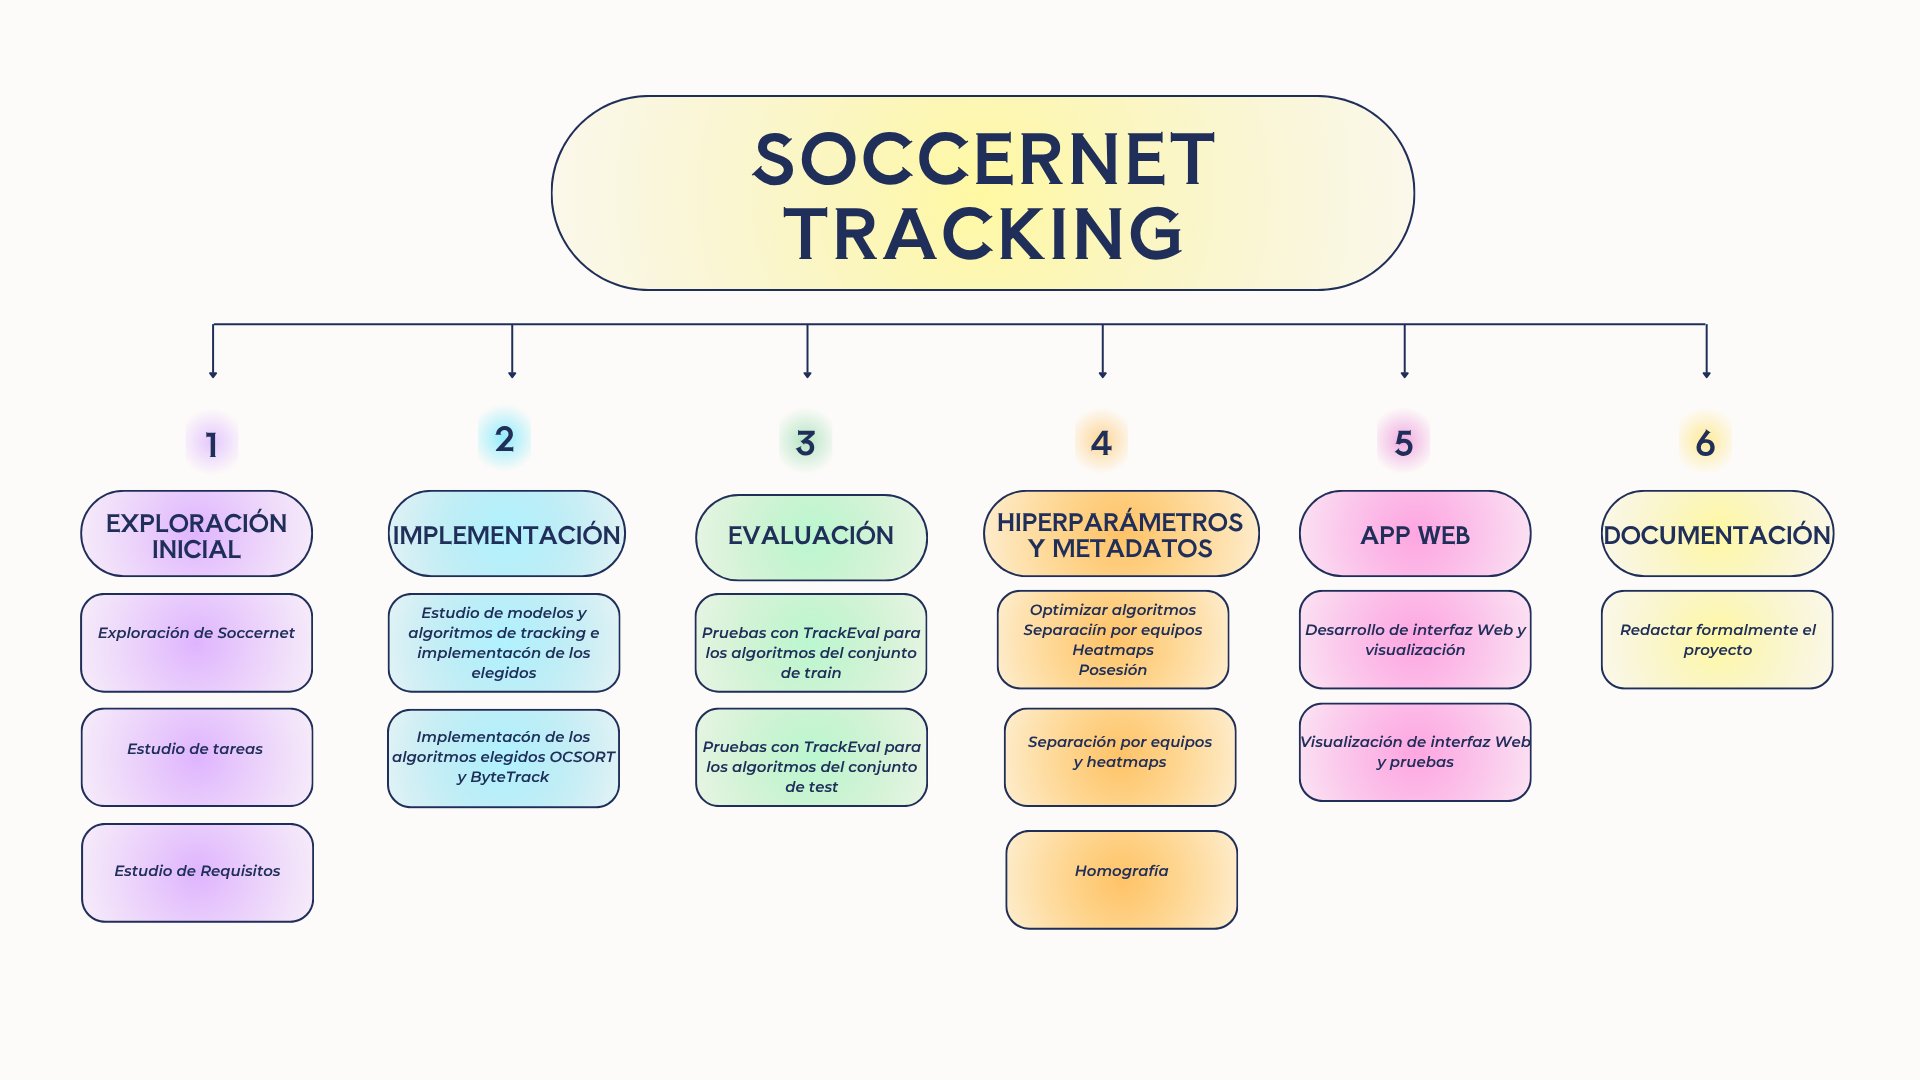
\includegraphics[width=0.98\textwidth]{figures/edt.png}
\caption{Estructura de descomposición del trabajo (EDT) del proyecto.}
\label{fig:gestion-edt}
\end{figure}

Cada paquete de trabajo del nivel inferior se detalla en el llamado
diccionario de la EDT, que recoge para cada uno su descripción, el rol
responsable y las horas dedicadas. La
Tabla~\ref{tab:gestion-edt-diccionario} recoge este diccionario completo,
ya consolidado con las horas realmente dedicadas al cierre del proyecto,
no solo las previstas en la planificación inicial, ampliadas en varios
paquetes por las causas descritas en la
sección~\ref{subsec:gestion-revision}; las horas por rol coinciden,
sumadas, con las horas totales por rol de la
Tabla~\ref{tab:gestion-costes-personal} de la
sección~\ref{sec:gestion-presupuesto}.

\begin{table}[htp]
\centering
\caption{Diccionario de la EDT: paquetes de trabajo, rol responsable y horas totales.}
\label{tab:gestion-edt-diccionario}
\small
\renewcommand{\arraystretch}{1.1}
\begin{tabular}{|p{1.0cm}|p{4.6cm}|p{3.6cm}|p{1.4cm}|}
\hline
\rowcolor{gray!25}
\textbf{ID} & \textbf{Paquete de trabajo} & \textbf{Rol} & \textbf{Horas} \\
\hline
0.1 & Traslados y reconfiguración del entorno de desarrollo (portátil,
  sobremesa, macOS) & Desarrollador & 10\,h \\
\hline
1.1 & Exploración de tareas de SoccerNet, valoración de alternativas y
  primeras pruebas de visualización & Ingeniero de Visión Artificial & 20\,h \\
\hline
1.2 & Comprensión del formato del dataset
  & Ingeniero de Visión Artificial & 5\,h \\
\hline
1.3 & Análisis de requisitos &
  Analista de software & 15\,h \\
\hline
2.1 & Implementación de ByteTrack y OC-SORT sobre \texttt{boxmot} &
  Ingeniero de Visión Artificial & 15\,h \\
\hline
2.2 & Filtrado geométrico del balón y ejecución batch sobre train &
  Ingeniero de Visión Artificial & 10\,h \\
\hline
3.1 & Integración de TrackEval y evaluación sobre train &
  Ingeniero de Visión Artificial & 20\,h \\
\hline
3.2 & Evaluación sobre test &
  Ingeniero de Visión Artificial & 10\,h \\
\hline
4.1 & Estudio de hiperparámetros de ByteTrack &
  Ingeniero de Visión Artificial & 10\,h \\
\hline
4.2 & Estudio de hiperparámetros de OC-SORT &
  Ingeniero de Visión Artificial & 10\,h \\
\hline
5.1 & Clasificación de equipos y mapas de calor (con y sin homografía) &
  Ingeniero de Visión Artificial & 20\,h \\
\hline
5.2 & Homografía real (distancia/velocidad) y posesión de balón &
  Ingeniero de Visión Artificial & 23\,h \\
\hline
6.1 & Desarrollo de la aplicación web & Desarrollador & 20\,h \\
\hline
6.2 & Ajustes y revisión de la aplicación web &
  Desarrollador & 15\,h \\
\hline
7.1 & Organización del repositorio y corrección de errores &
  Desarrollador & 20\,h \\
\hline
8.1 & Redacción de la memoria & Jefe de proyecto & 90\,h \\
\hline
\rowcolor{gray!10}
 & \textbf{Total} & & \textbf{313\,h} \\
\hline
\end{tabular}
\end{table}

Esta cifra final, superior a las 300\,h estimadas en la planificación
inicial (sección~\ref{sec:gestion-planificacion}), no es un error de
previsión menor sino el reflejo de cómo evolucionó realmente el proyecto:
la sección~\ref{subsec:gestion-revision} detalla las causas concretas de
esa desviación de horas.

\section{Planificación temporal}
\label{sec:gestion-planificacion}

\subsection{Elaboración del plan de trabajo}

El proyecto arrancó a finales de febrero de 2026 con una toma de contacto
muy preliminar con la web de SoccerNet, seguida en marzo de una fase ya
informal pero más concreta de exploración de las distintas tareas de su
ecosistema (sección~\ref{sec:gestion-fases}), antes de comprometerse
formalmente con el tracking como tarea del proyecto a finales de abril. A
partir de ahí,
la disponibilidad de tiempo fue muy variable a lo largo de los meses
siguientes debido al solapamiento con la época de exámenes del resto de
asignaturas del grado. Esta irregularidad, previsible desde el principio
dado el calendario académico, condicionó la forma de planificar: en lugar
de repartir el esfuerzo de manera uniforme mes a mes, la planificación
inicial --elaborada ya en abril, una vez elegida la tarea-- asumió
explícitamente periodos de baja dedicación durante los exámenes de mayo y
concentró el grueso del trabajo en los meses sin solapamiento académico.
Esa planificación inicial fue la siguiente:

\begin{itemize}
  \item \textbf{Abril (20--30)} -- Arranque. Exploración de tareas y
        elección definitiva de la tarea (tracking). Primeros scripts de
        visualización. Implementación de ByteTrack y OC-SORT. Ejecución
        sobre las secuencias de entrenamiento. Preparación del entorno de
        evaluación con TrackEval.
  \item \textbf{Mayo} -- Ritmo muy reducido por exámenes (aproximadamente
        20 horas en todo el mes, con prácticamente inactividad entre el 7 y
        el 25). Objetivo: obtener las primeras métricas reales y mantener
        un feedback constante de seguimiento con el tutor.
  \item \textbf{Junio} -- Núcleo del proyecto (unas 120 horas estimadas):
        evaluación en test, estudio de hiperparámetros, pipeline de
        metadatos, y comienzo de la redacción de la memoria en paralelo.
  \item \textbf{Julio} -- Cierre (unas 80 horas estimadas): desarrollo de la
        aplicación web y finalización de la memoria.
\end{itemize}

La estimación total de esta planificación inicial fue de unas 300 horas,
que incluían un margen reservado para imprevistos y tiempo de tutorías,
con una fecha de entrega prevista a finales de julio
de 2026. La Tabla~\ref{tab:gestion-gantt} representa esta misma
planificación en forma de cronograma, situando cada fase del proyecto
(sección~\ref{sec:gestion-fases}) sobre el mes o los meses en que se ha
concentrado su desarrollo, incluyendo la revisión de la planificación
descrita en la sección~\ref{subsec:gestion-revision}.

\begin{table}[htp]
\centering
\caption[Cronograma real del proyecto por fase y mes]{Cronograma real
del proyecto por fase y mes. El tono claro distingue actividad parcial o
de repaso/retoque frente al grueso del trabajo de cada fase (tono
oscuro).}
\label{tab:gestion-gantt}
\renewcommand{\arraystretch}{1.3}
\begin{tabular}{|p{3.2cm}|c|c|c|c|c|c|c|c|c|}
\hline
\rowcolor{gray!25}
\textbf{Fase} & \textbf{Feb} & \textbf{Mar} & \textbf{Abr} & \textbf{May} & \textbf{Jun} & \textbf{Jul} & \textbf{Ago} & \textbf{Sep} & \textbf{Oct} \\
\hline
1. Exploración inicial & \cellcolor{blue!10}\checkmark & \cellcolor{blue!25}\checkmark & & & & & & & \\
\hline
2. Implementación de trackers & & & \cellcolor{blue!25}\checkmark & & & & & & \\
\hline
3. Evaluación & & & \cellcolor{blue!25}\checkmark & \cellcolor{blue!25}\checkmark & & & & & \\
\hline
4. Estudio de hiperparámetros & & & & & \cellcolor{blue!25}\checkmark & & & & \\
\hline
5. Pipeline de metadatos & & & & & \cellcolor{blue!25}\checkmark & & & & \\
\hline
6. Aplicación web & & & & & & & \cellcolor{blue!25}\checkmark & \cellcolor{blue!10}\checkmark & \\
\hline
7. Redacción de la memoria & & & & & \cellcolor{blue!10}\checkmark & \cellcolor{blue!10}\checkmark & \cellcolor{blue!25}\checkmark & \cellcolor{blue!25}\checkmark & \cellcolor{blue!10}\checkmark \\
\hline
\end{tabular}
\end{table}

Como refleja el cronograma, la fase 1 tampoco se concentra en un único
mes: arranca con una toma de contacto muy ligera en febrero y se
convierte en la exploración real, ya concreta, en marzo. La fase 7
sigue un patrón parecido: arranca de forma parcial en junio y julio, se
convierte en
el grueso real del trabajo en agosto y septiembre, y se cierra con una
revisión final en octubre antes de la entrega. La fase 6 sigue un patrón
similar a menor escala: el desarrollo principal de la aplicación web se
concentra en agosto, con un repaso final en septiembre --organización del
repositorio y revisión de la interfaz-- ya en paralelo a la recta final
de la redacción
(sección~\ref{subsec:impl-web-frontend} del
capítulo~\ref{cap:implementacion}).

\subsection{Seguimiento y monitorización}
\label{subsec:gestion-monitorizacion}

\FloatBarrier

El seguimiento del tiempo dedicado a este proyecto se ha apoyado en una
herramienta de \emph{time-tracking} dedicada, Clockify (Figuras~\ref{fig:gestion-monitorizacion}
a~\ref{fig:gestion-clockify-sep-p2}), complementada por el documento de
anotaciones descrito en la sección~\ref{sec:gestion-metodologia} y por el
historial de commits del repositorio Git, cuya fecha permite además
reconstruir con razonable precisión cuándo se completó cada hito. Las
horas totales por paquete de trabajo de la Tabla~\ref{tab:gestion-edt-diccionario}
y la desviación cuantificada en la sección~\ref{subsec:gestion-revision}
proceden de esta herramienta. Para cada mes se muestran, en dos capturas
sucesivas, el reparto diario de horas junto con la categoría de proyecto
a la que pertenecen (\emph{Implementación}, \emph{Investigación} o
\emph{Redacción}), y el desglose completo de las tareas individuales
registradas con su tiempo dedicado.

\begin{figure}[htp]
\centering
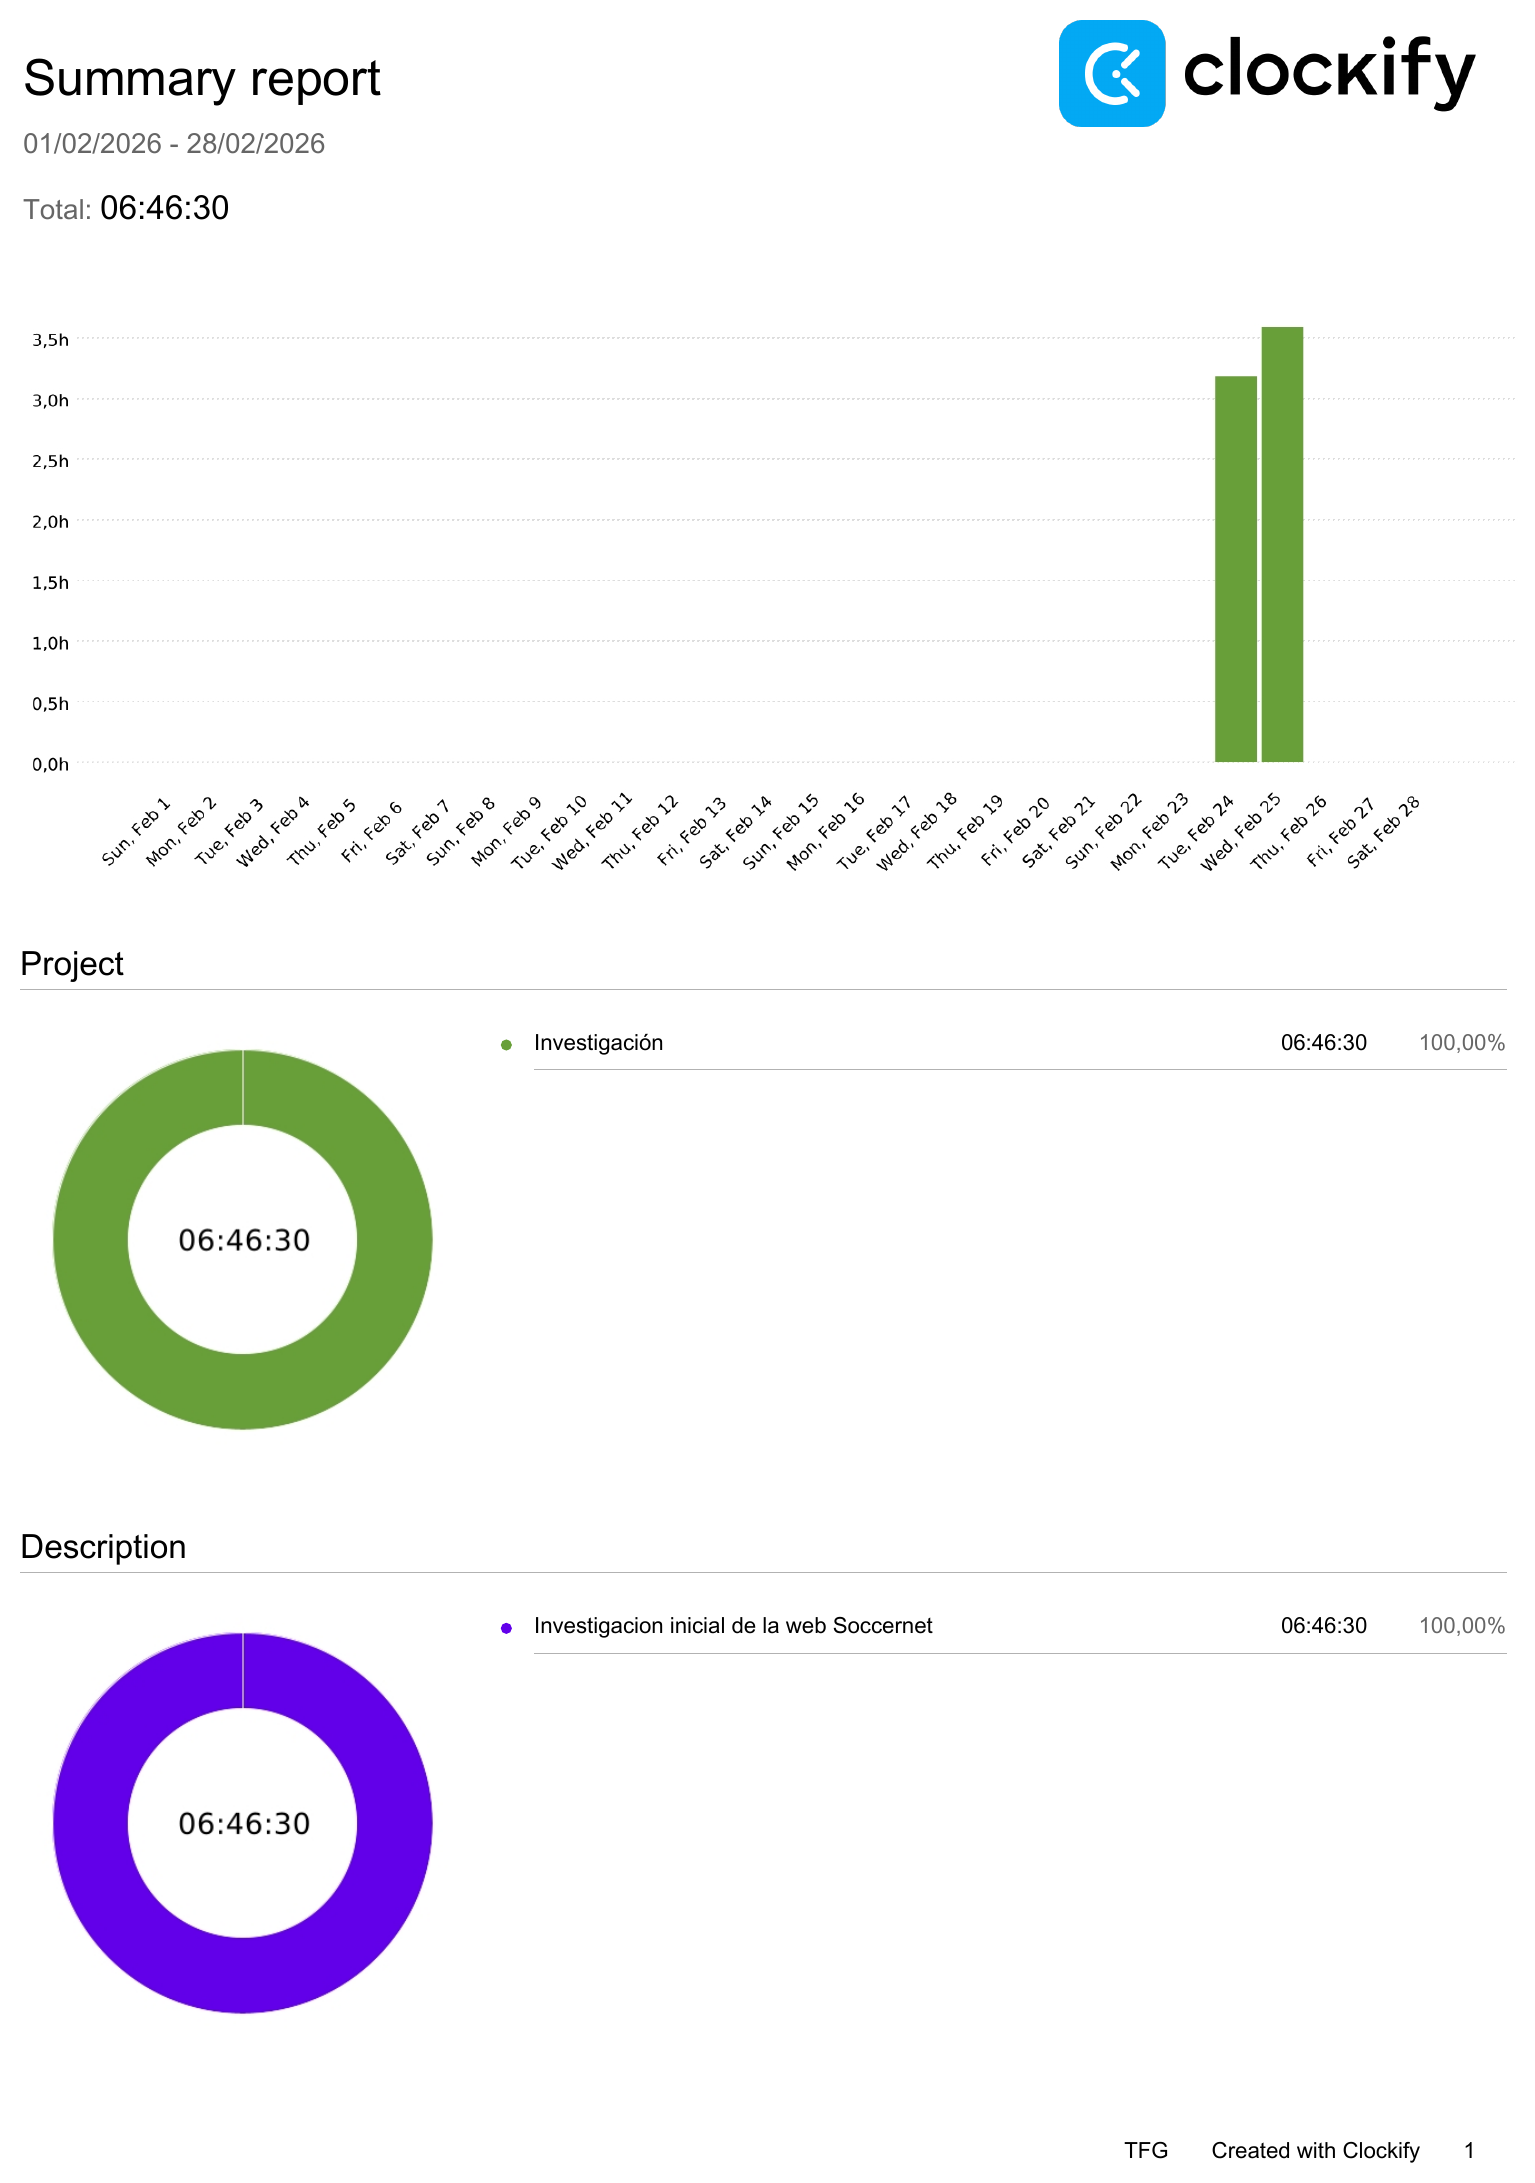
\includegraphics[height=0.72\textheight, keepaspectratio]{figures/clockify_02_2026_p1.png}
\caption{Febrero 2026: apenas 7\,h registradas, una toma de contacto muy
preliminar con la web de SoccerNet, antes de arrancar con la exploración
ya concreta de marzo.}
\label{fig:gestion-monitorizacion}
\end{figure}

\FloatBarrier

\begin{figure}[htp]
\centering
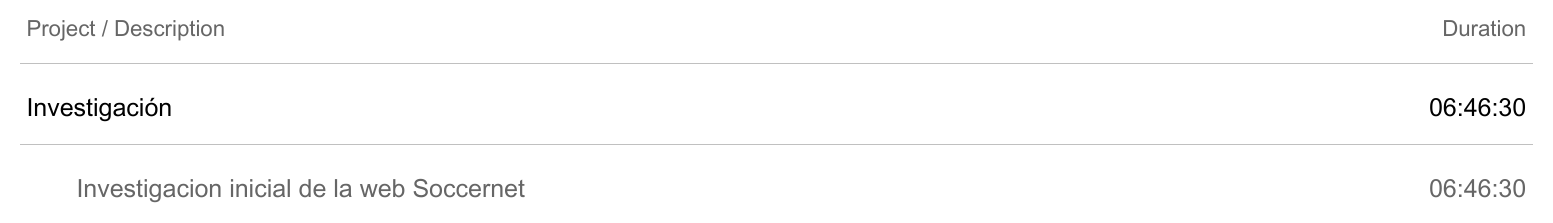
\includegraphics[width=0.92\textwidth, keepaspectratio]{figures/clockify_02_2026_p2.png}
\caption{Febrero 2026: única tarea registrada en todo el mes.}
\end{figure}

\FloatBarrier

\begin{figure}[htp]
\centering
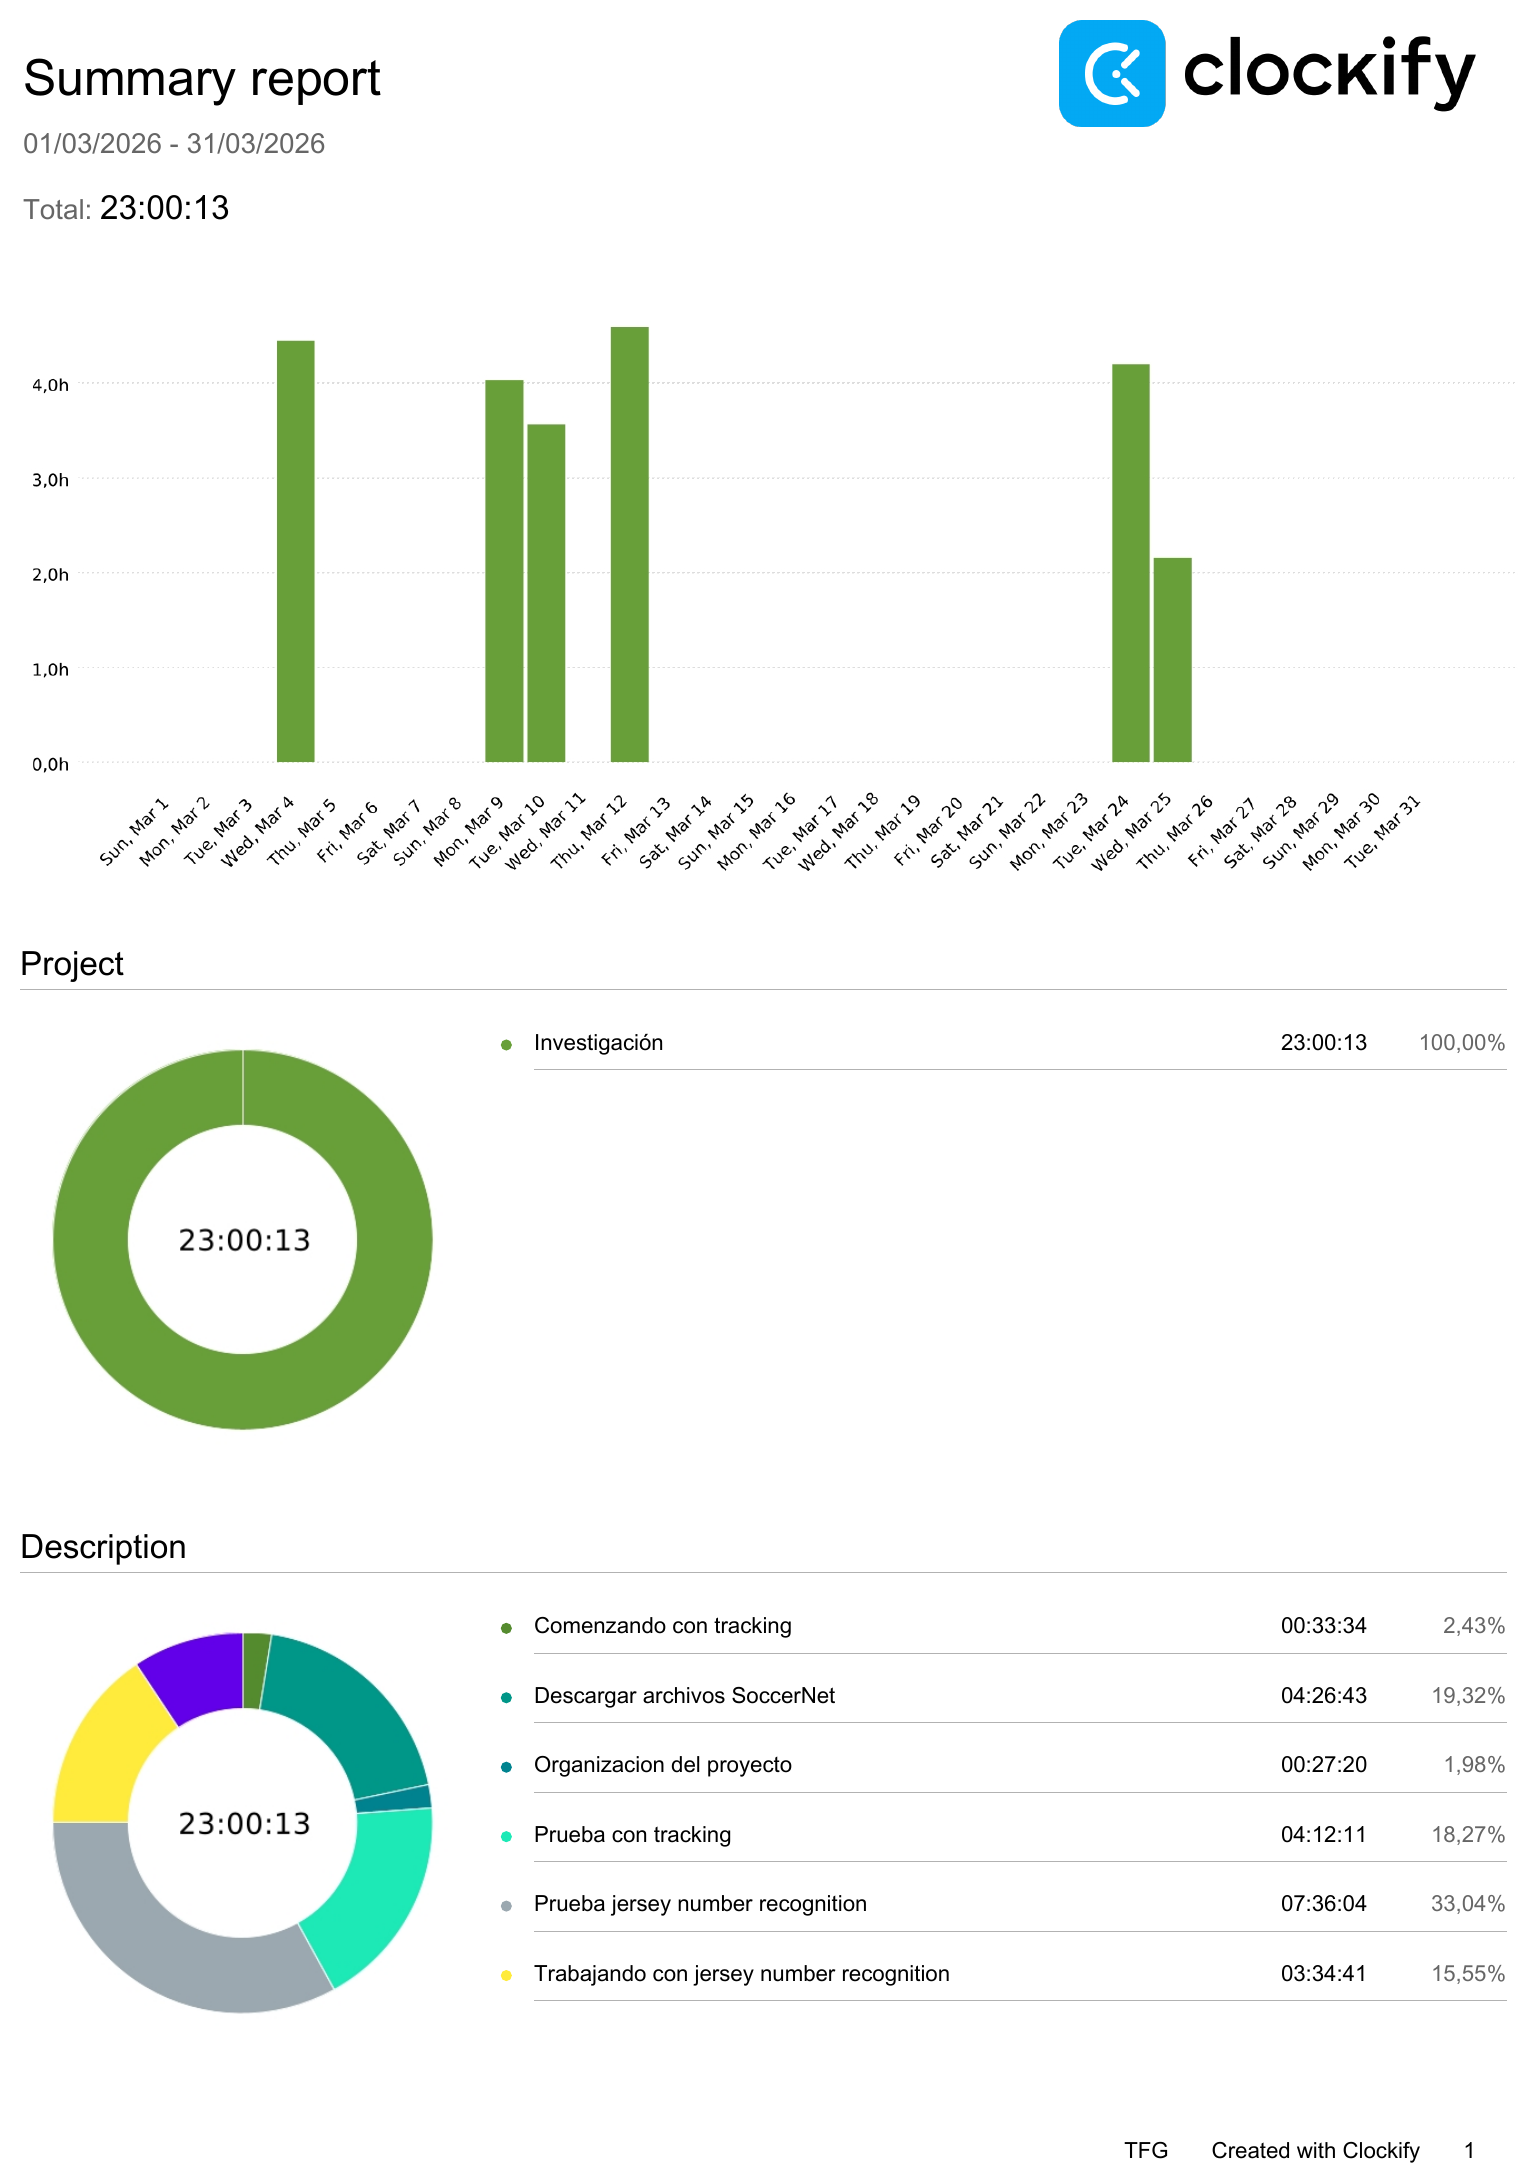
\includegraphics[height=0.72\textheight, keepaspectratio]{figures/clockify_03_2026_p1.png}
\caption{Marzo 2026: unas 23\,h registradas.}
\end{figure}

\FloatBarrier

\begin{figure}[htp]
\centering
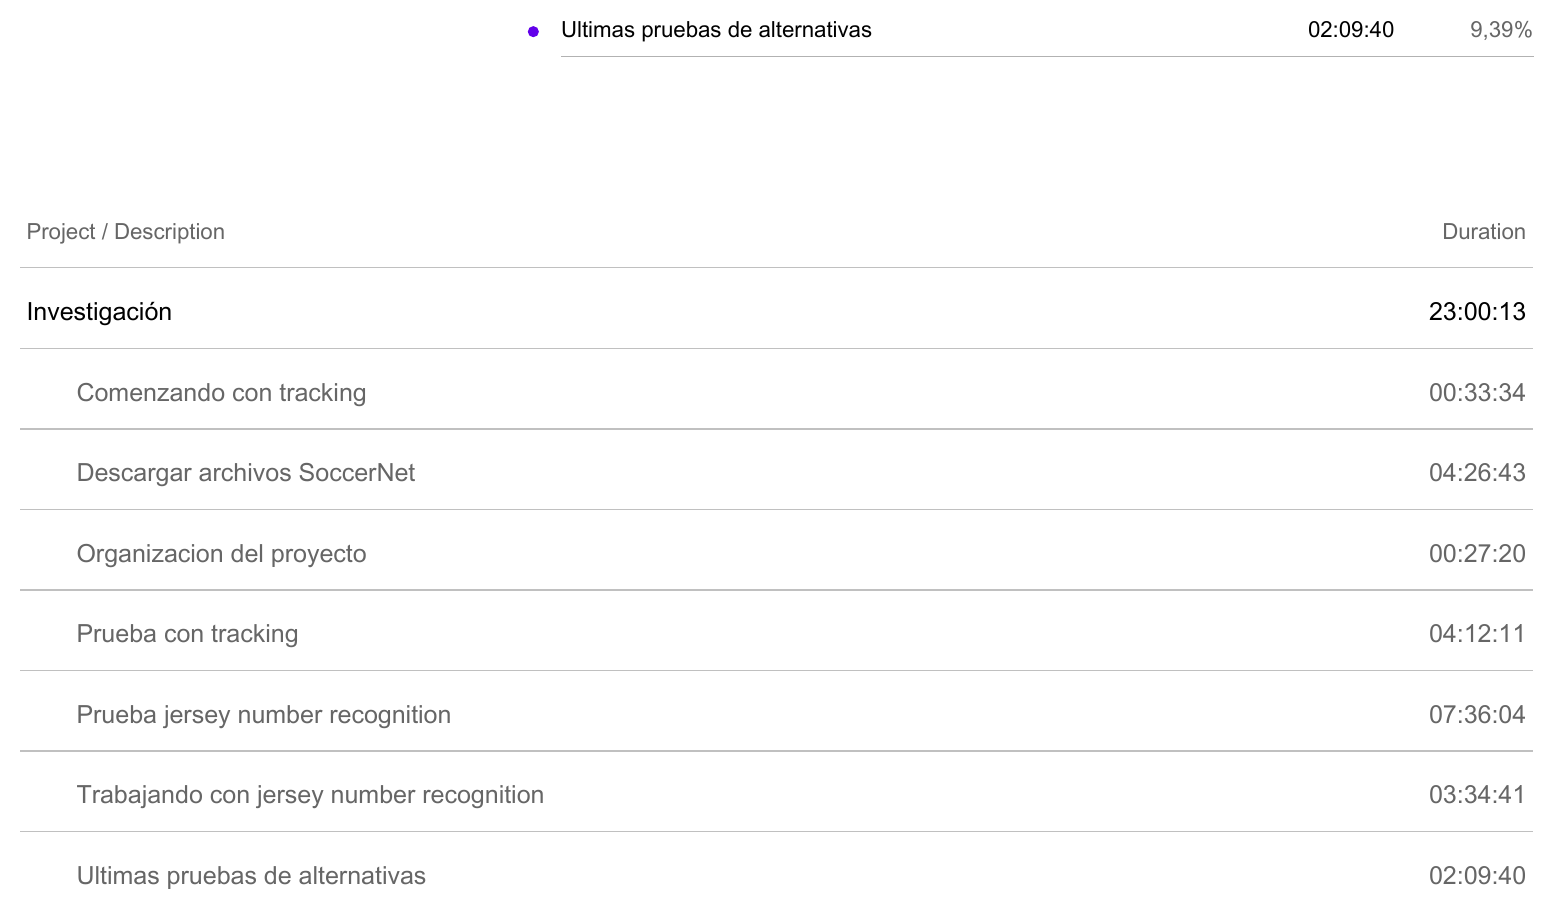
\includegraphics[width=0.92\textwidth, keepaspectratio]{figures/clockify_03_2026_p2.png}
\caption{Marzo 2026: desglose completo de las tareas de exploración
inicial y el tiempo dedicado a cada una.}
\end{figure}

\FloatBarrier

\begin{figure}[htp]
\centering
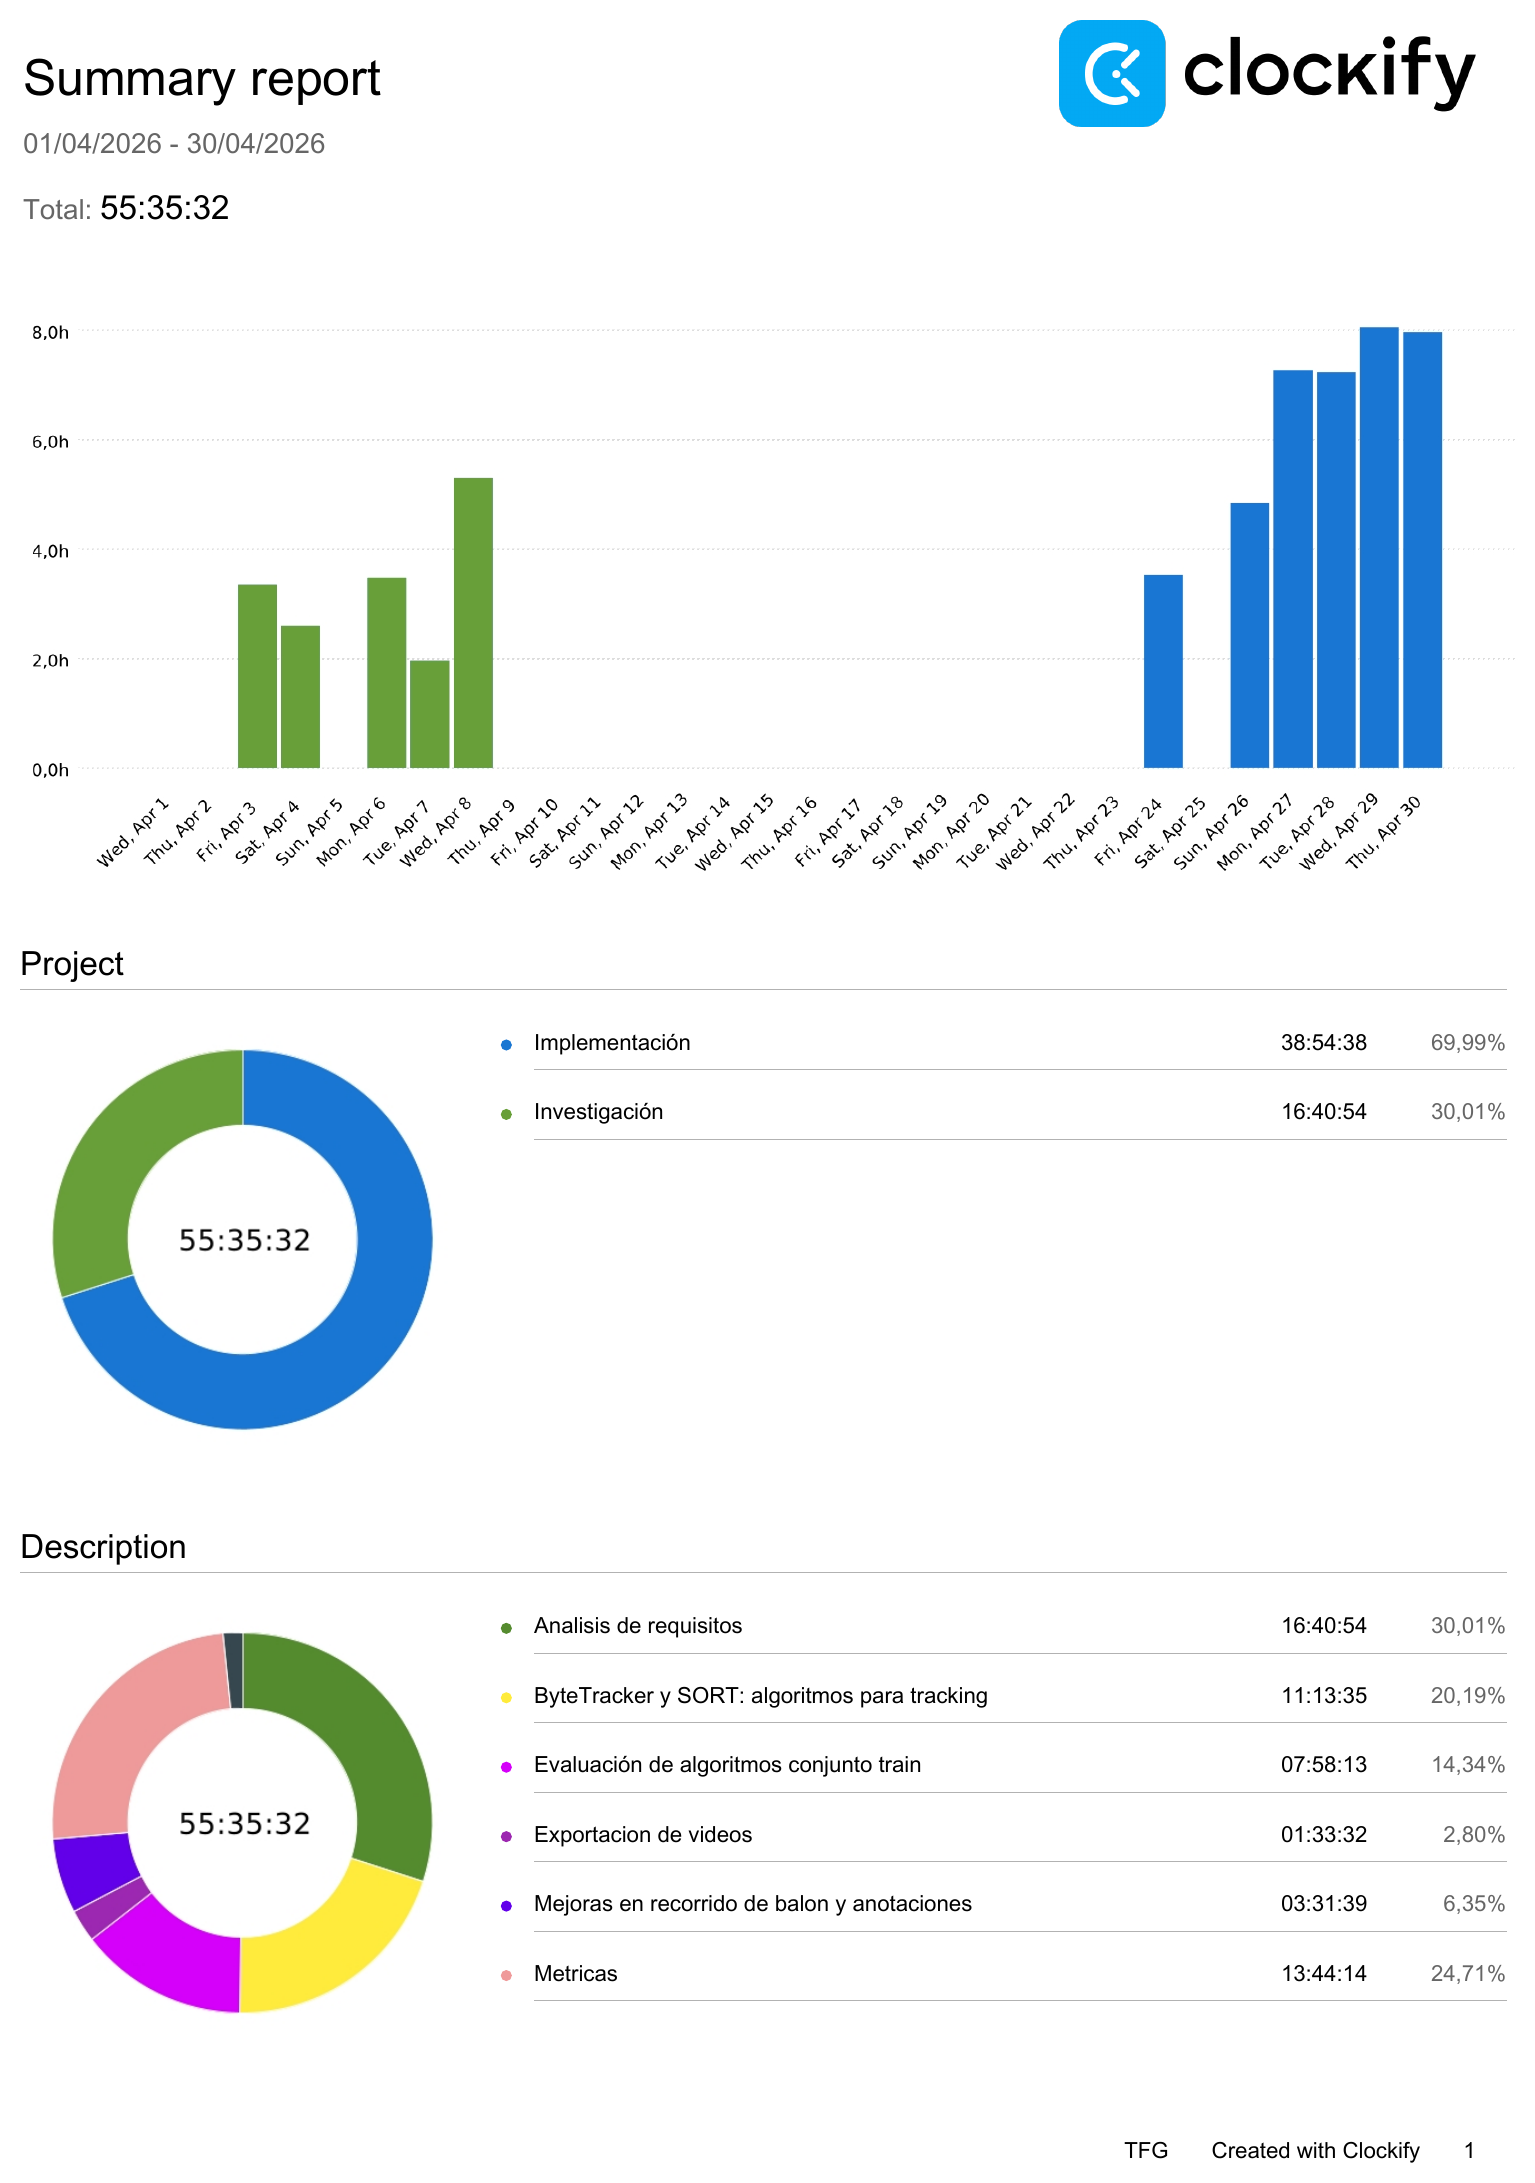
\includegraphics[height=0.72\textheight, keepaspectratio]{figures/clockify_04_2026_p1.png}
\caption{Abril 2026: unas 56\,h registradas.}
\end{figure}

\FloatBarrier

\begin{figure}[htp]
\centering
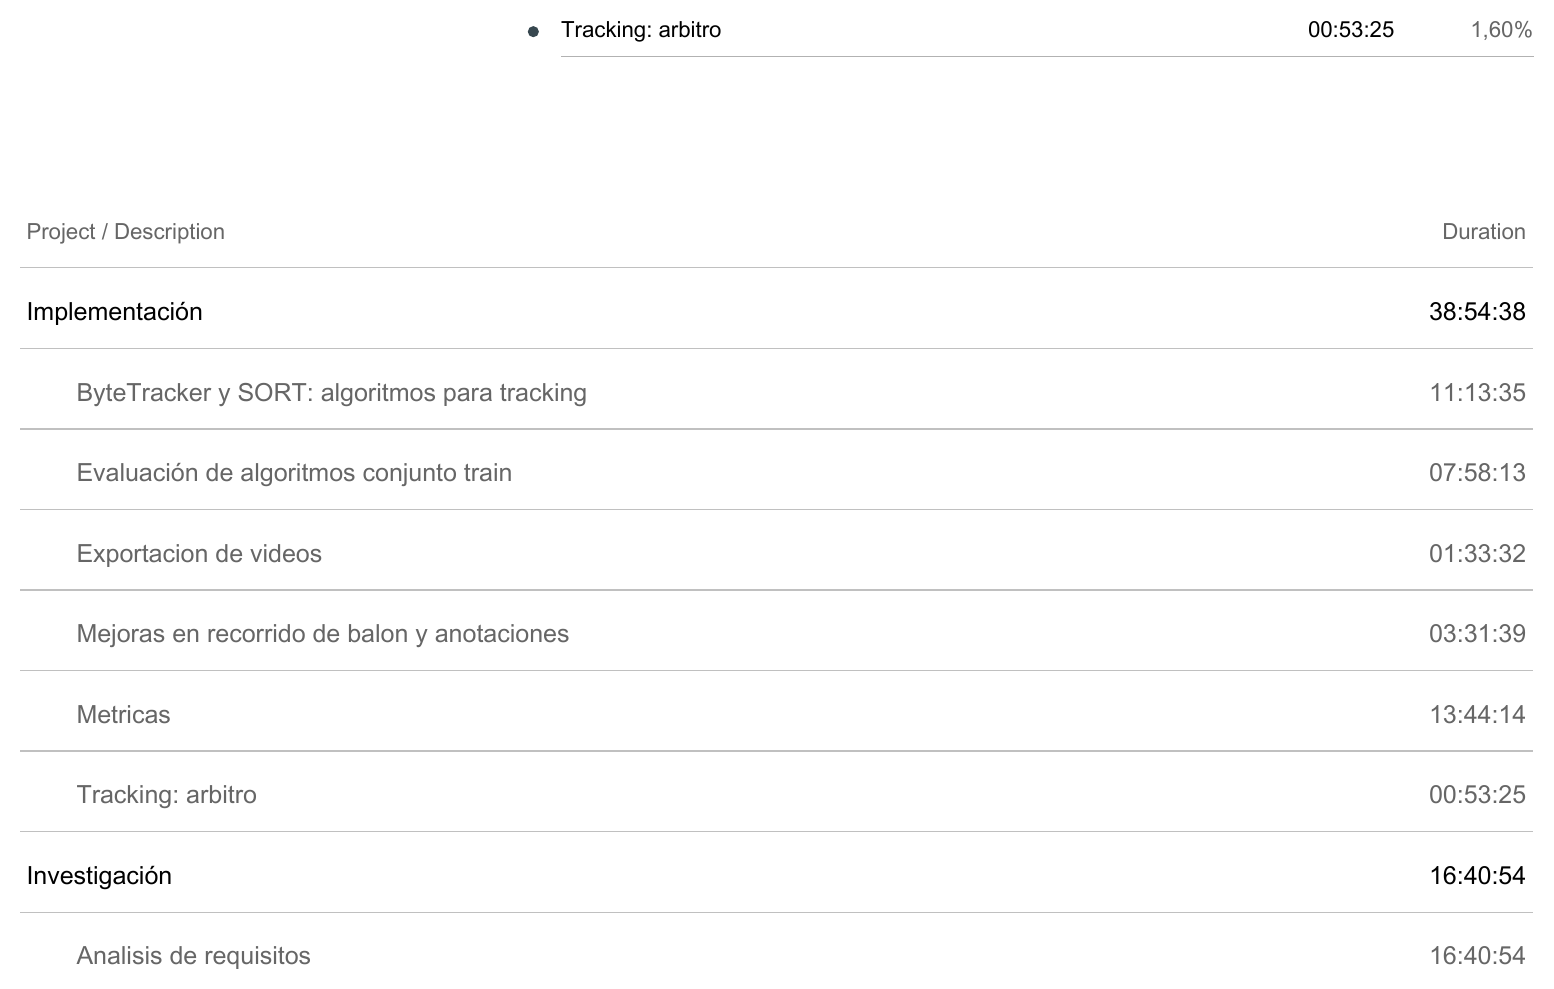
\includegraphics[width=0.92\textwidth, keepaspectratio]{figures/clockify_04_2026_p2.png}
\caption{Abril 2026: desglose completo de tareas.}
\end{figure}

\FloatBarrier

\begin{figure}[htp]
\centering
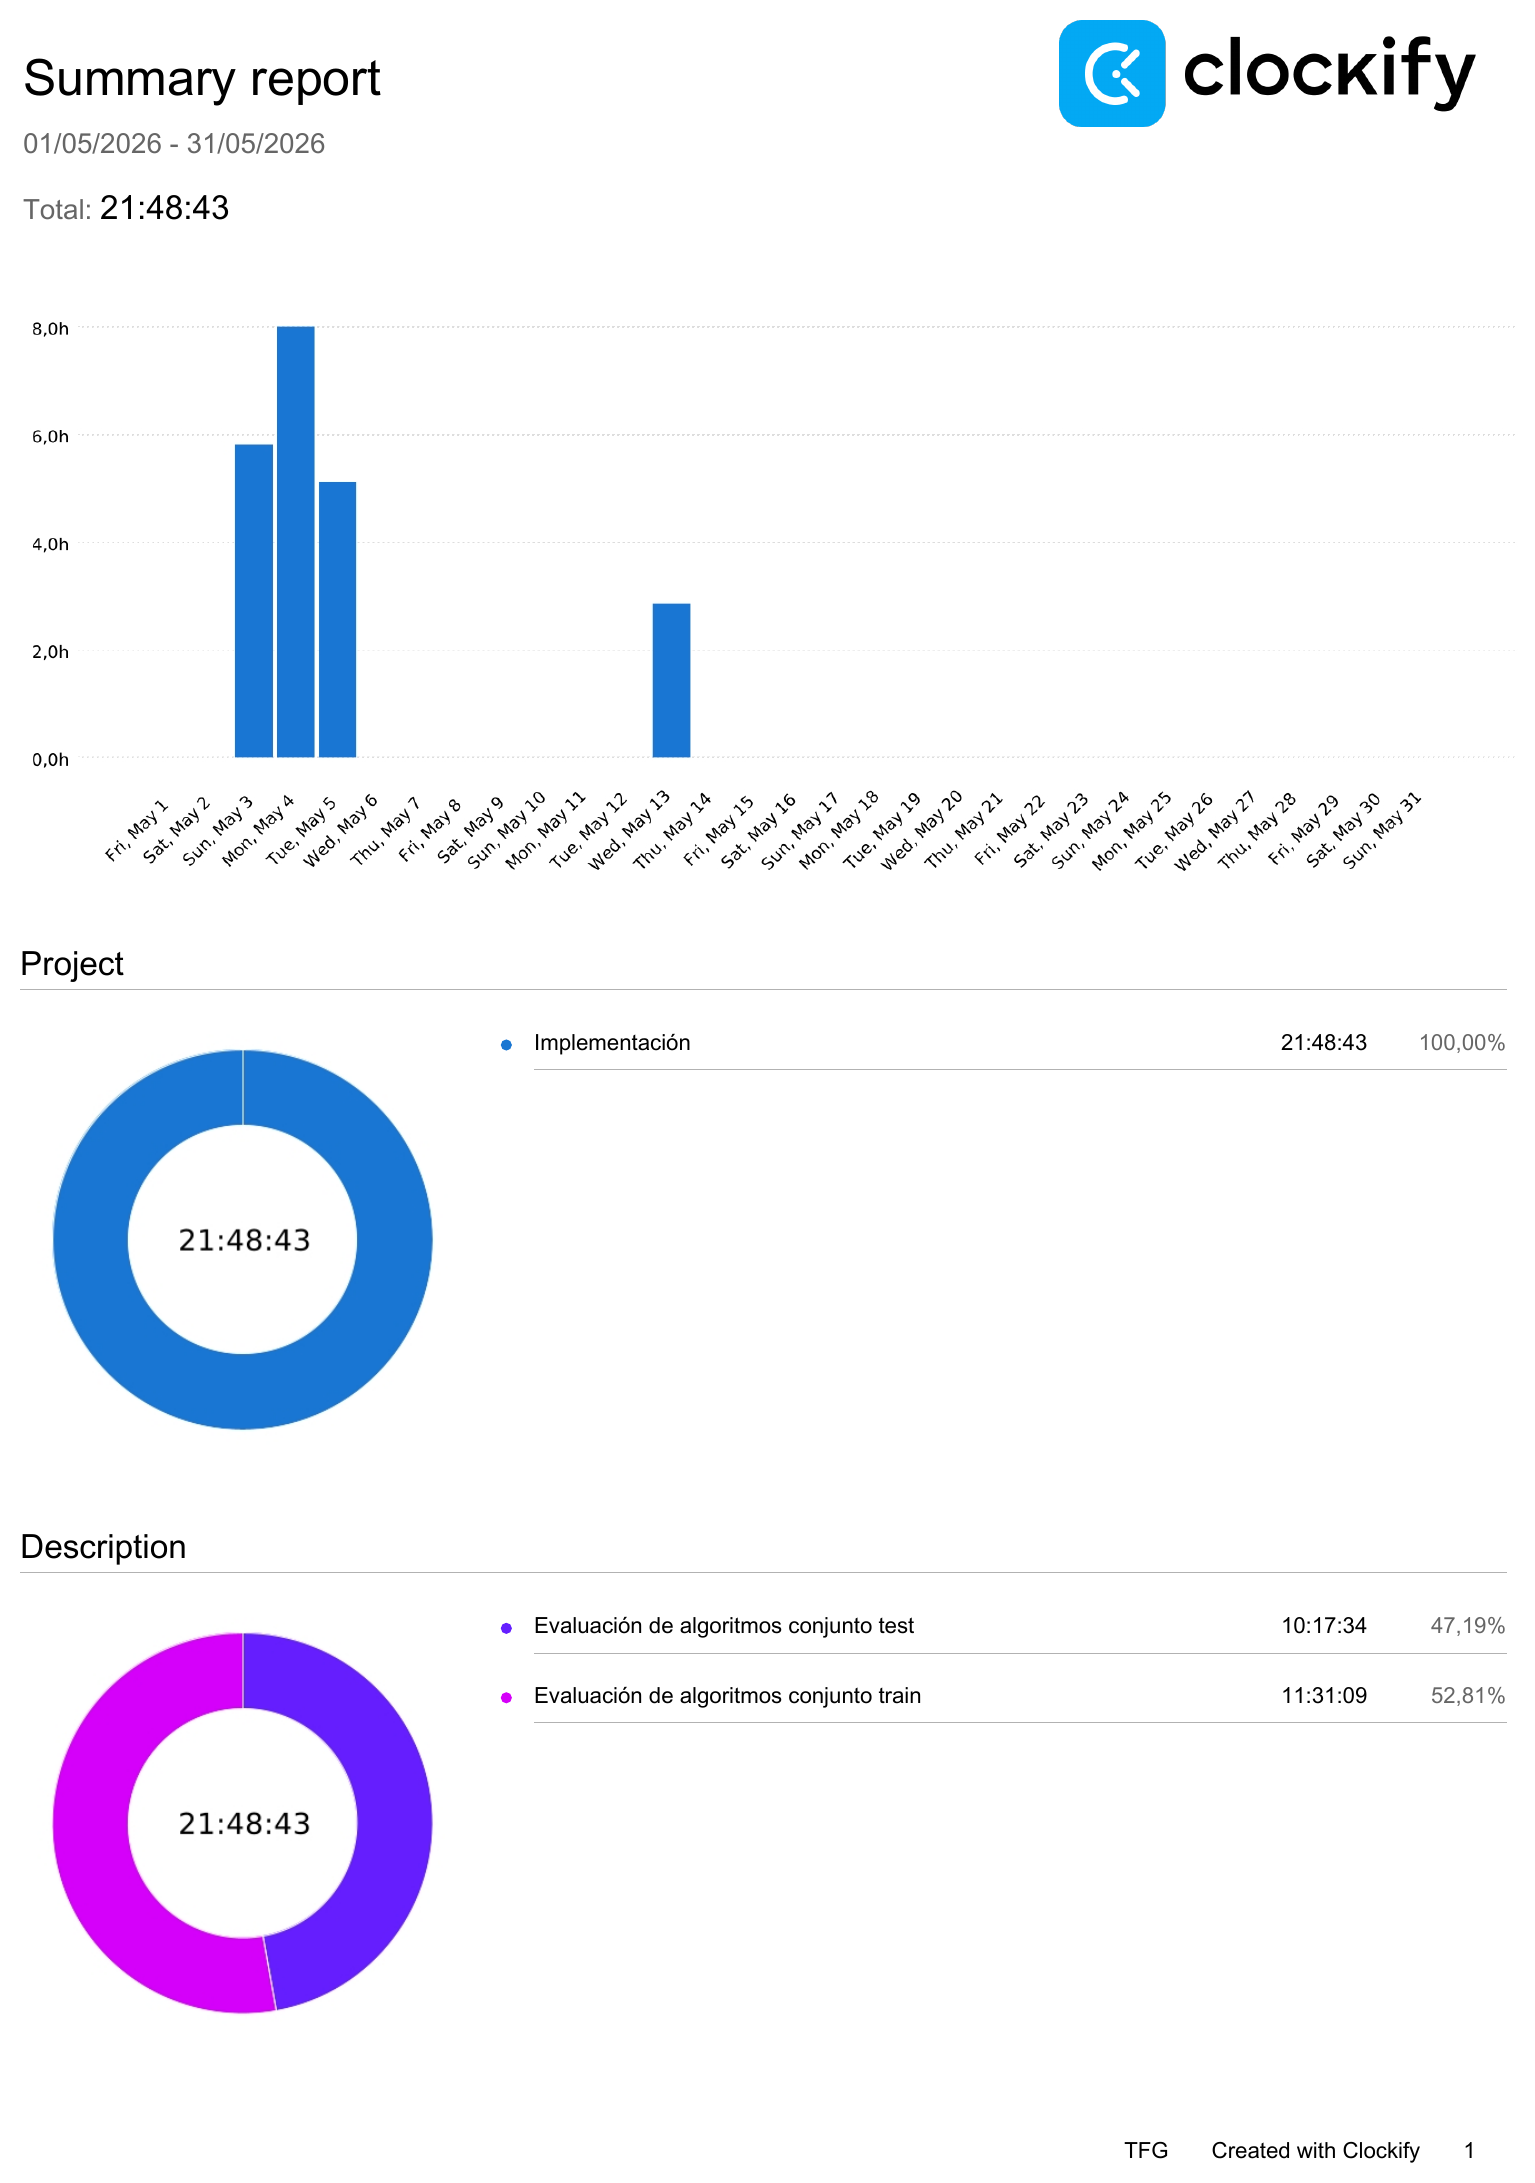
\includegraphics[height=0.72\textheight, keepaspectratio]{figures/clockify_05_2026_p1.png}
\caption{Mayo 2026: unas 22\,h registradas.}
\end{figure}

\FloatBarrier

\begin{figure}[htp]
\centering
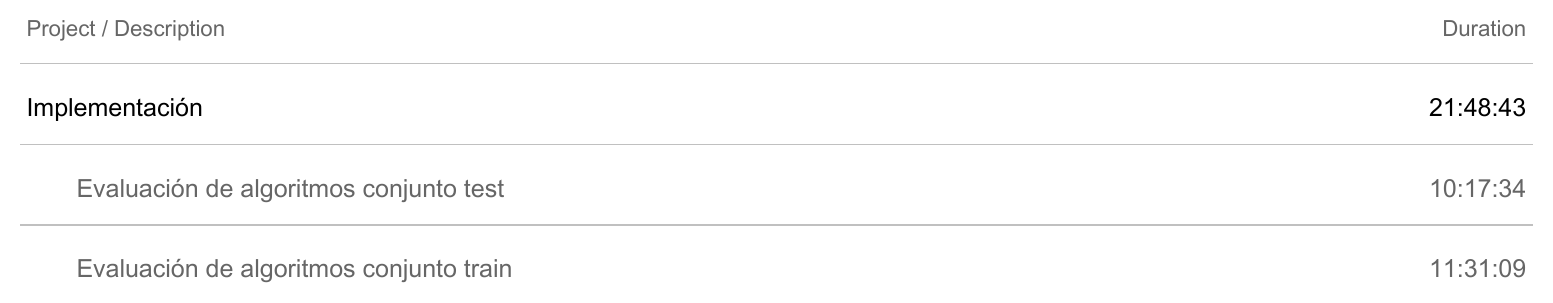
\includegraphics[width=0.92\textwidth, keepaspectratio]{figures/clockify_05_2026_p2.png}
\caption{Mayo 2026: desglose completo de las dos tareas de evaluación
realizadas.}
\end{figure}

\FloatBarrier

\begin{figure}[htp]
\centering
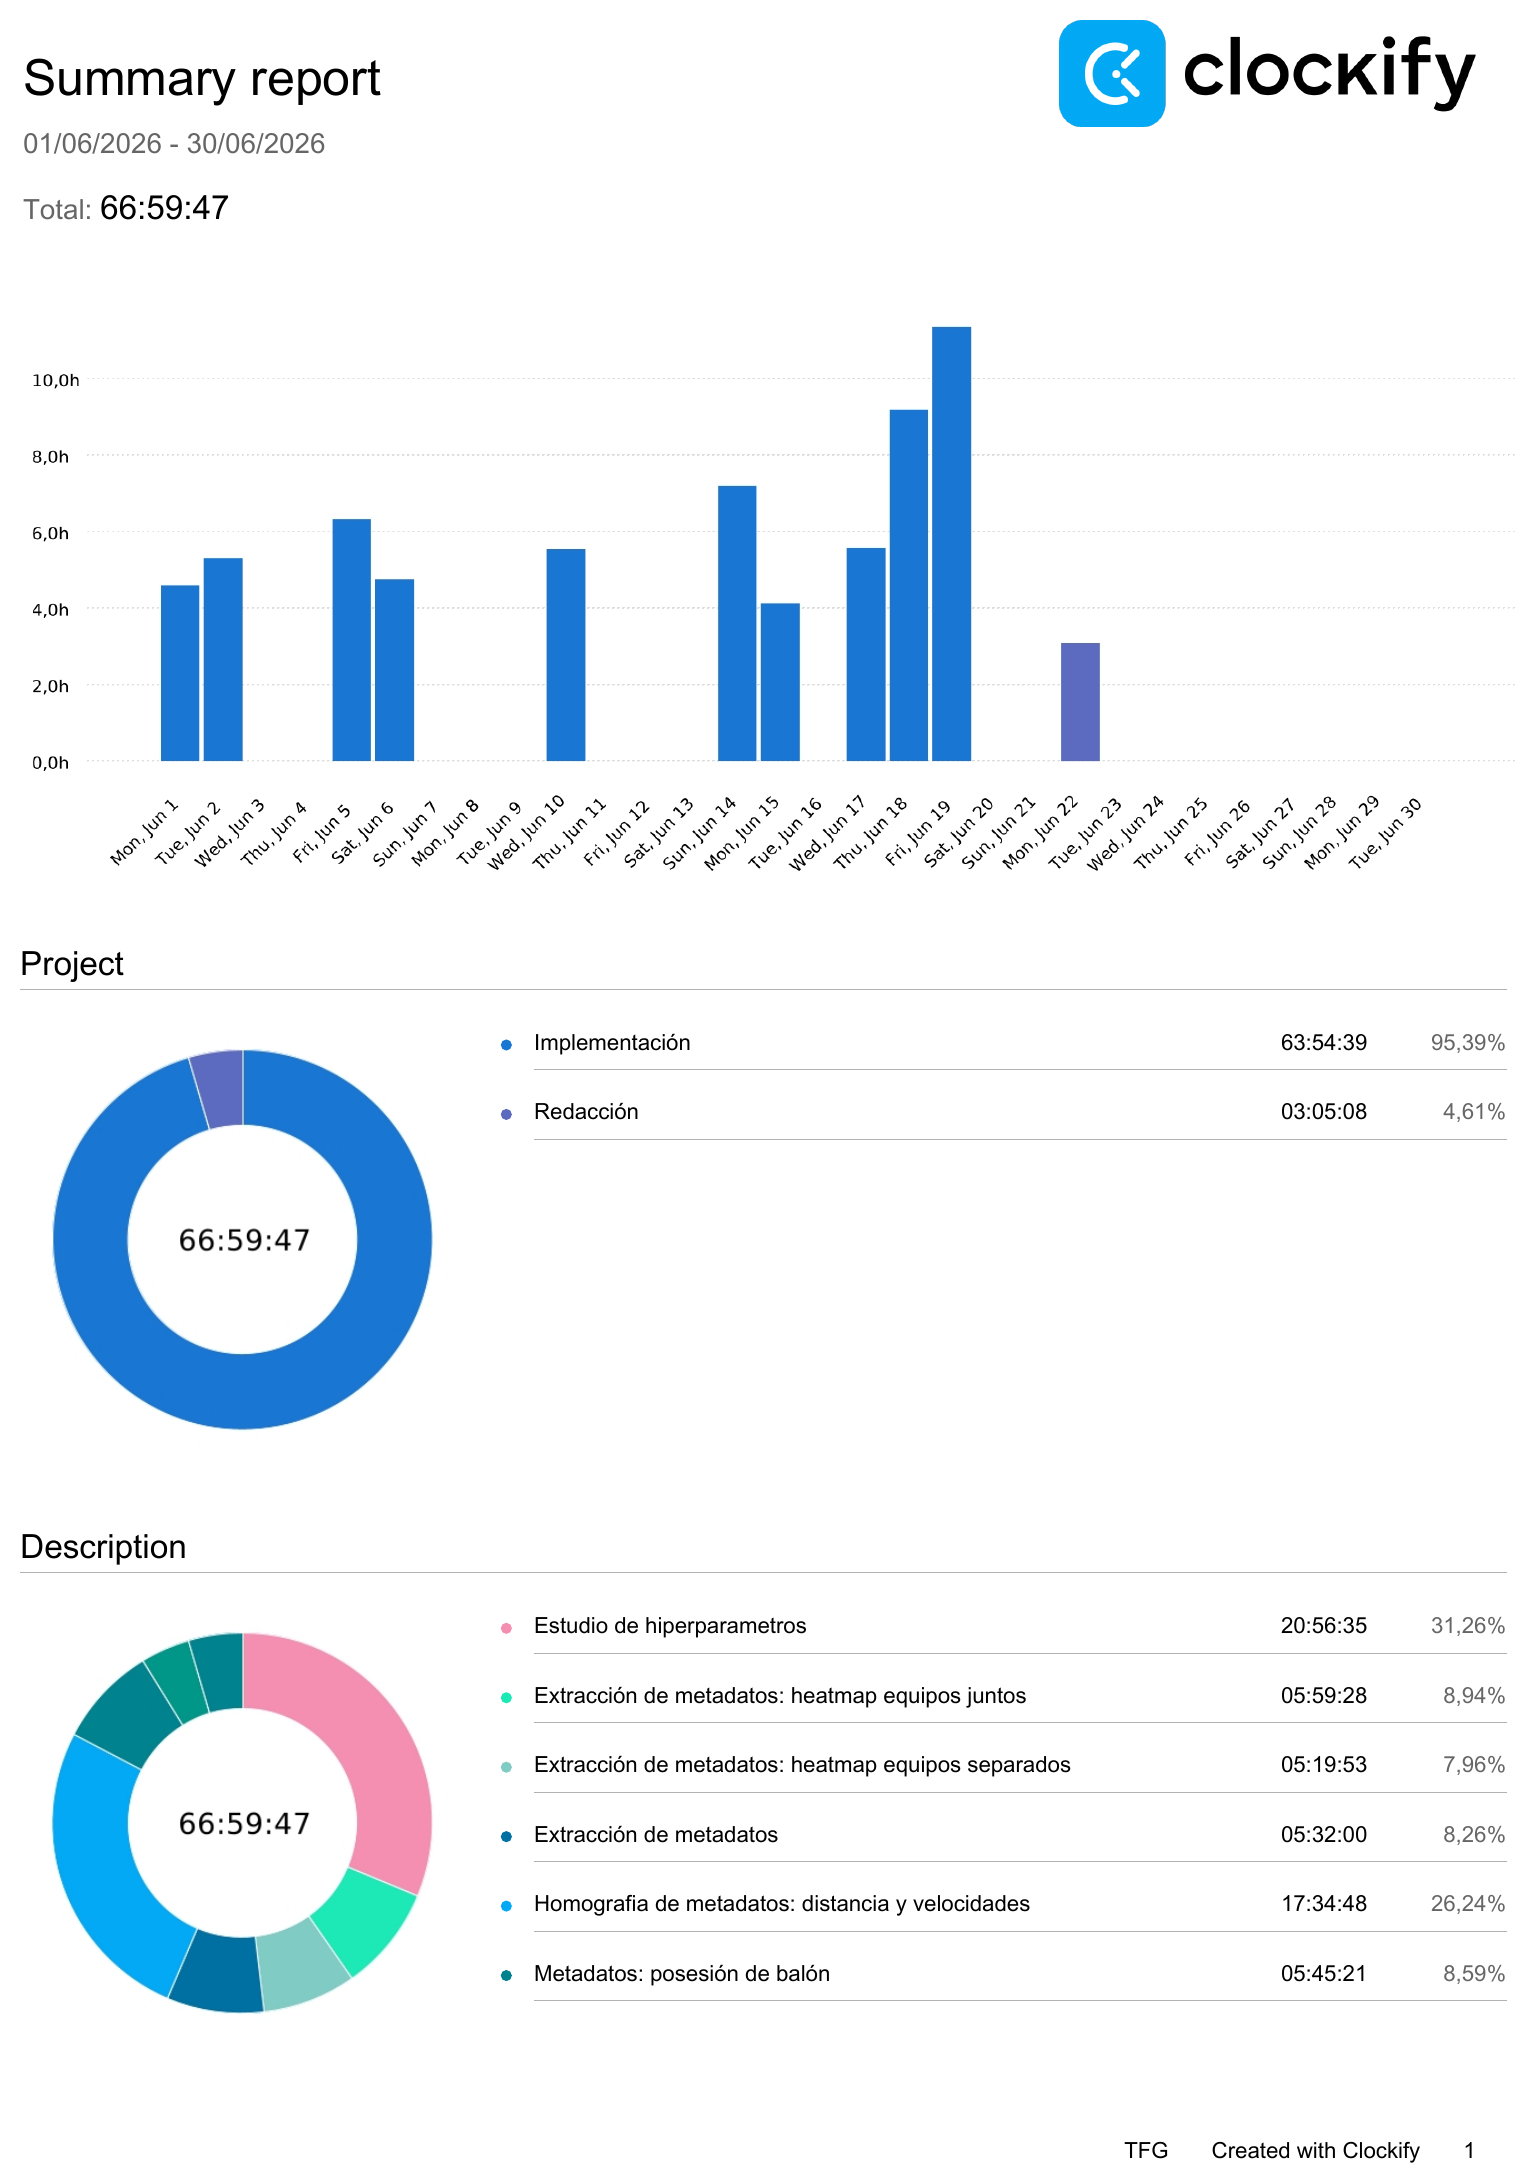
\includegraphics[height=0.72\textheight, keepaspectratio]{figures/clockify_06_2026_p1.png}
\caption{Junio 2026: cerca de 67\,h registradas.}
\end{figure}

\FloatBarrier

\begin{figure}[htp]
\centering
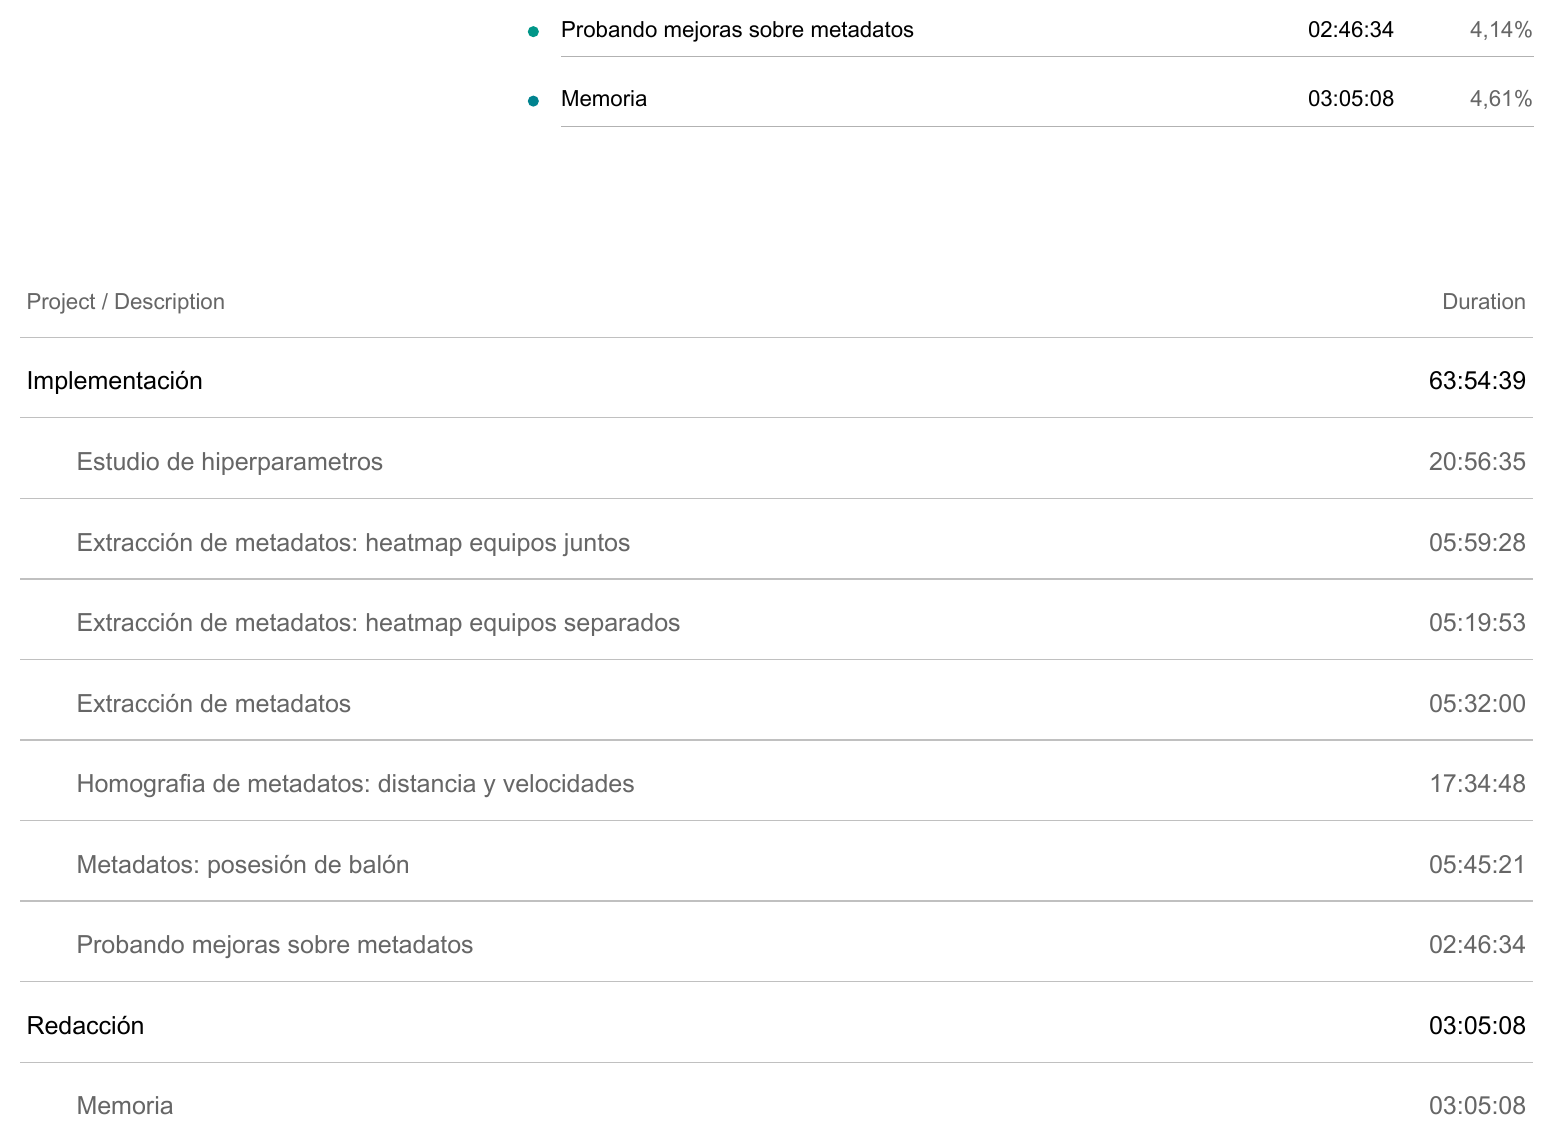
\includegraphics[width=0.92\textwidth, keepaspectratio]{figures/clockify_06_2026_p2.png}
\caption{Junio 2026: desglose completo de tareas.}
\end{figure}

\FloatBarrier

\begin{figure}[htp]
\centering
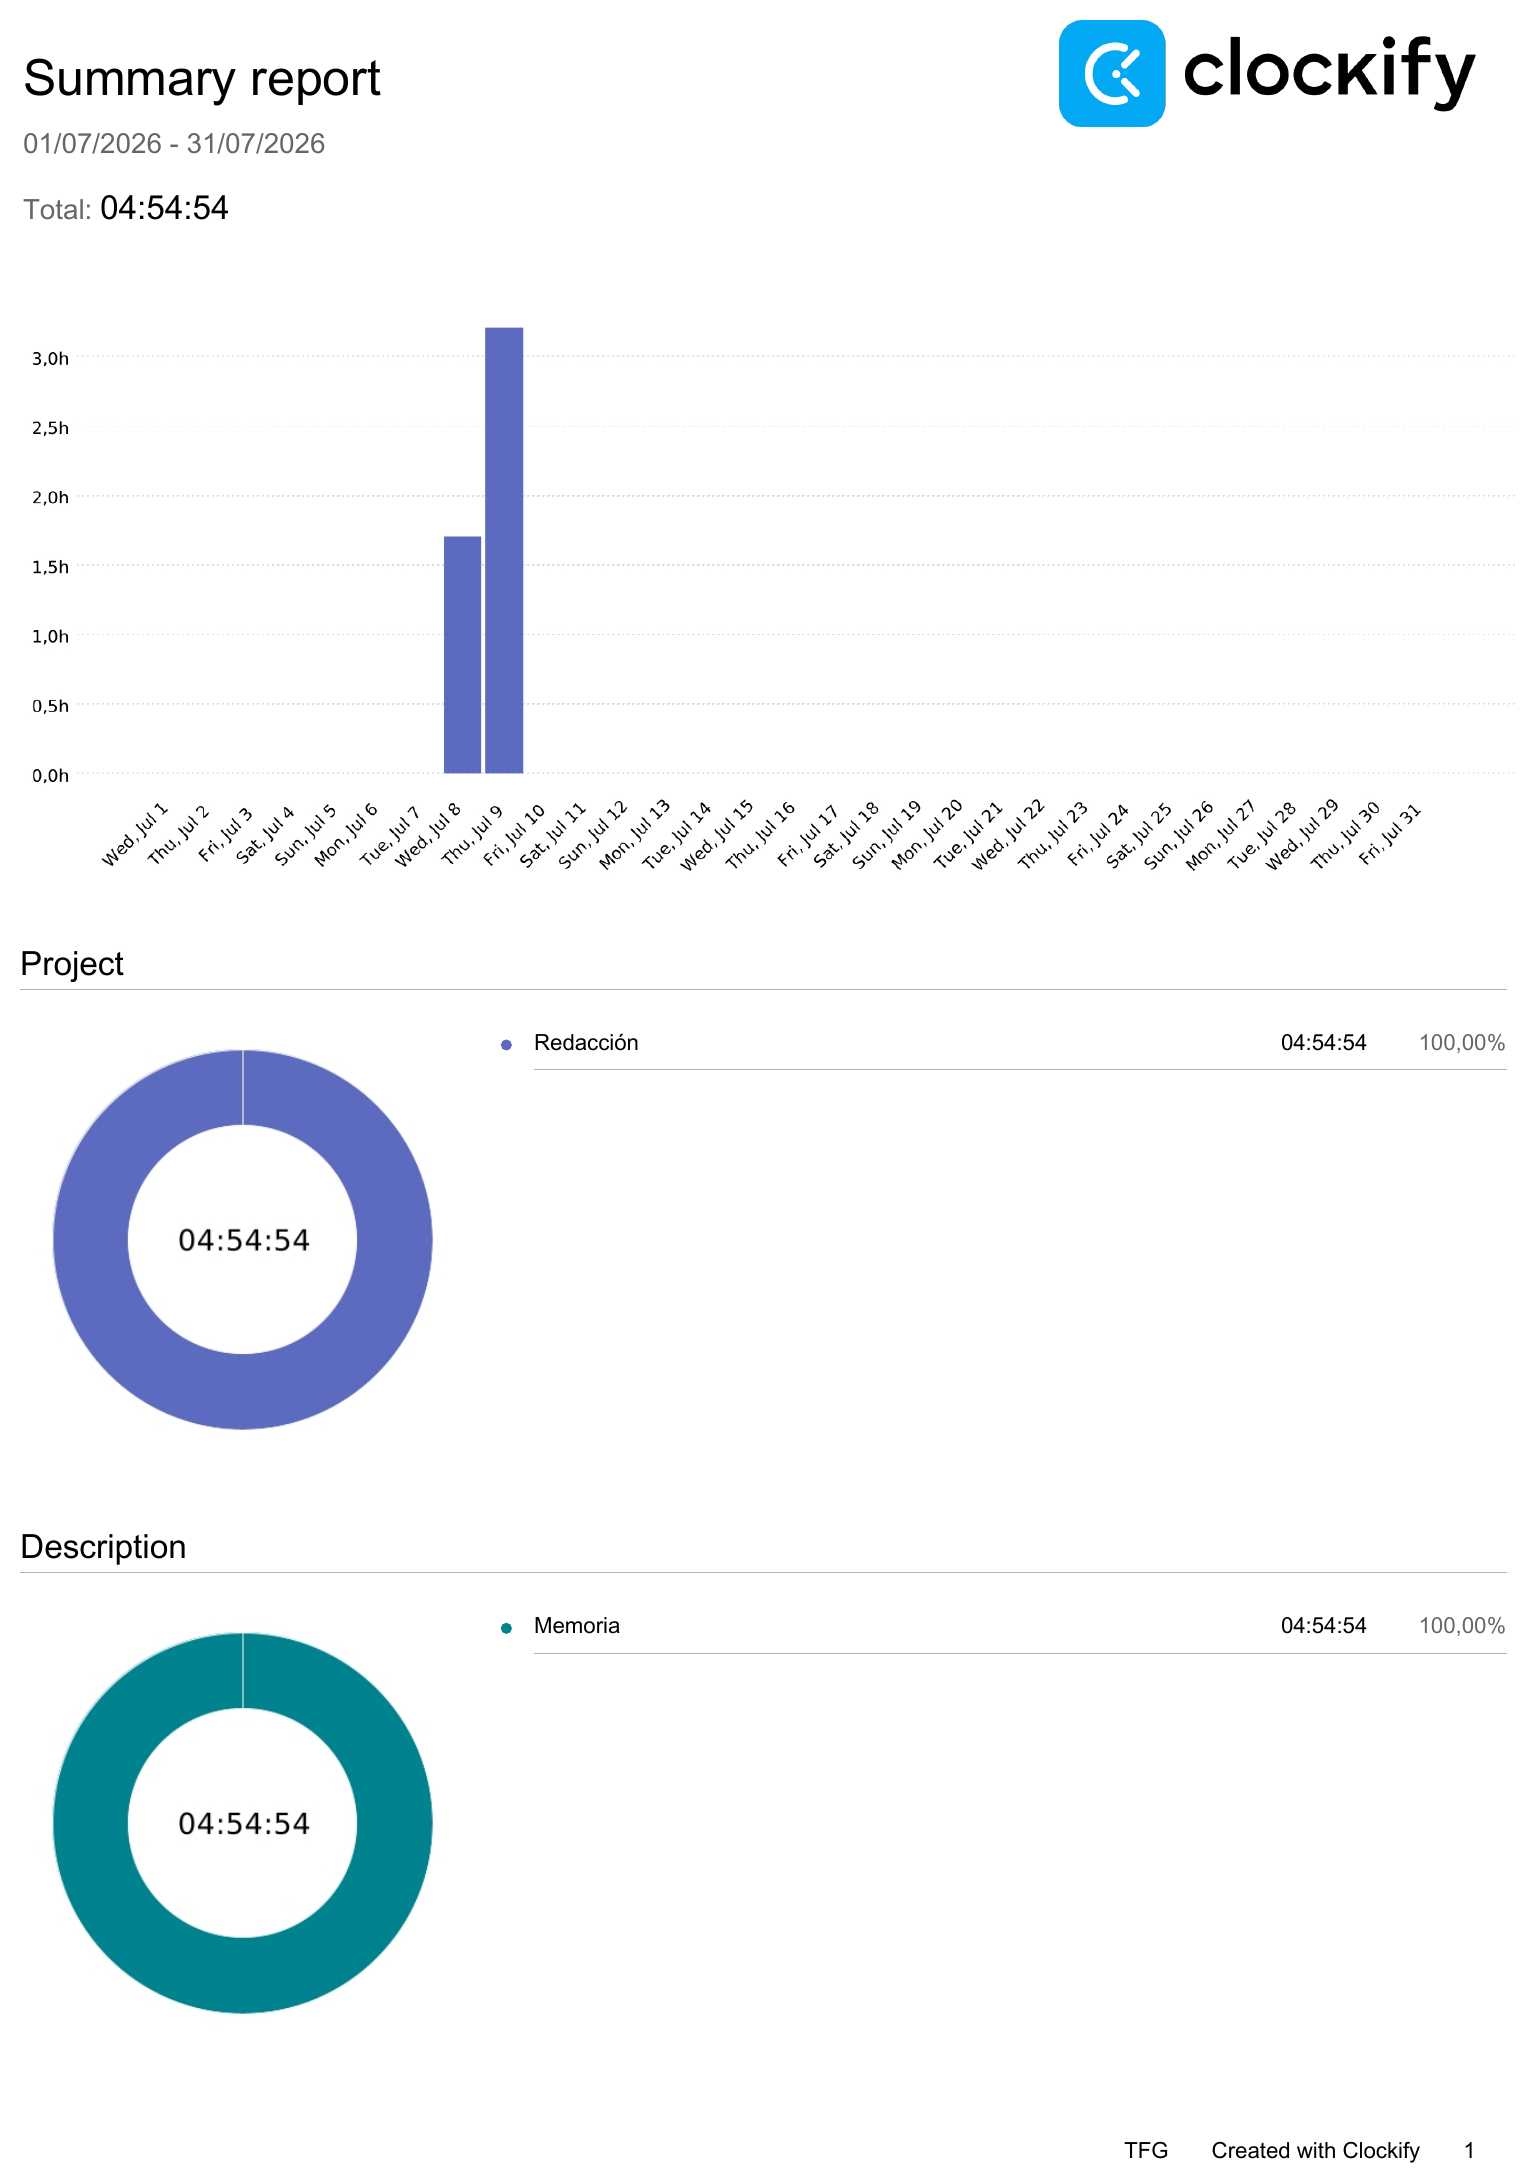
\includegraphics[height=0.72\textheight, keepaspectratio]{figures/clockify_07_2026_p1.png}
\caption{Julio 2026: apenas 5\,h registradas.}
\end{figure}

\FloatBarrier

\begin{figure}[htp]
\centering
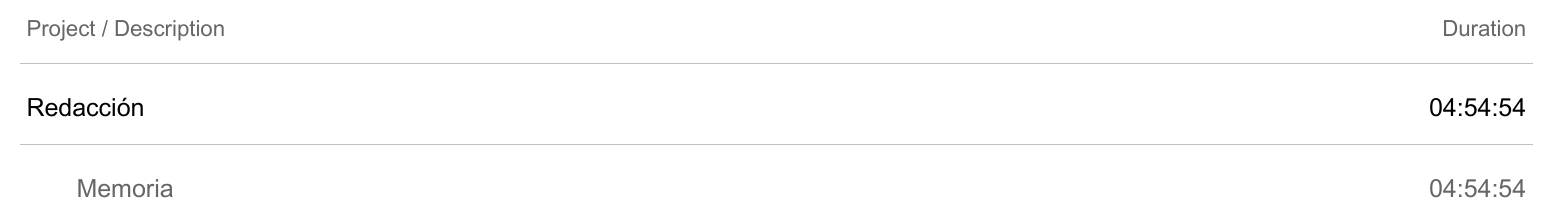
\includegraphics[width=0.92\textwidth, keepaspectratio]{figures/clockify_07_2026_p2.png}
\caption{Julio 2026: única tarea registrada en todo el mes.}
\end{figure}

\FloatBarrier

\begin{figure}[htp]
\centering
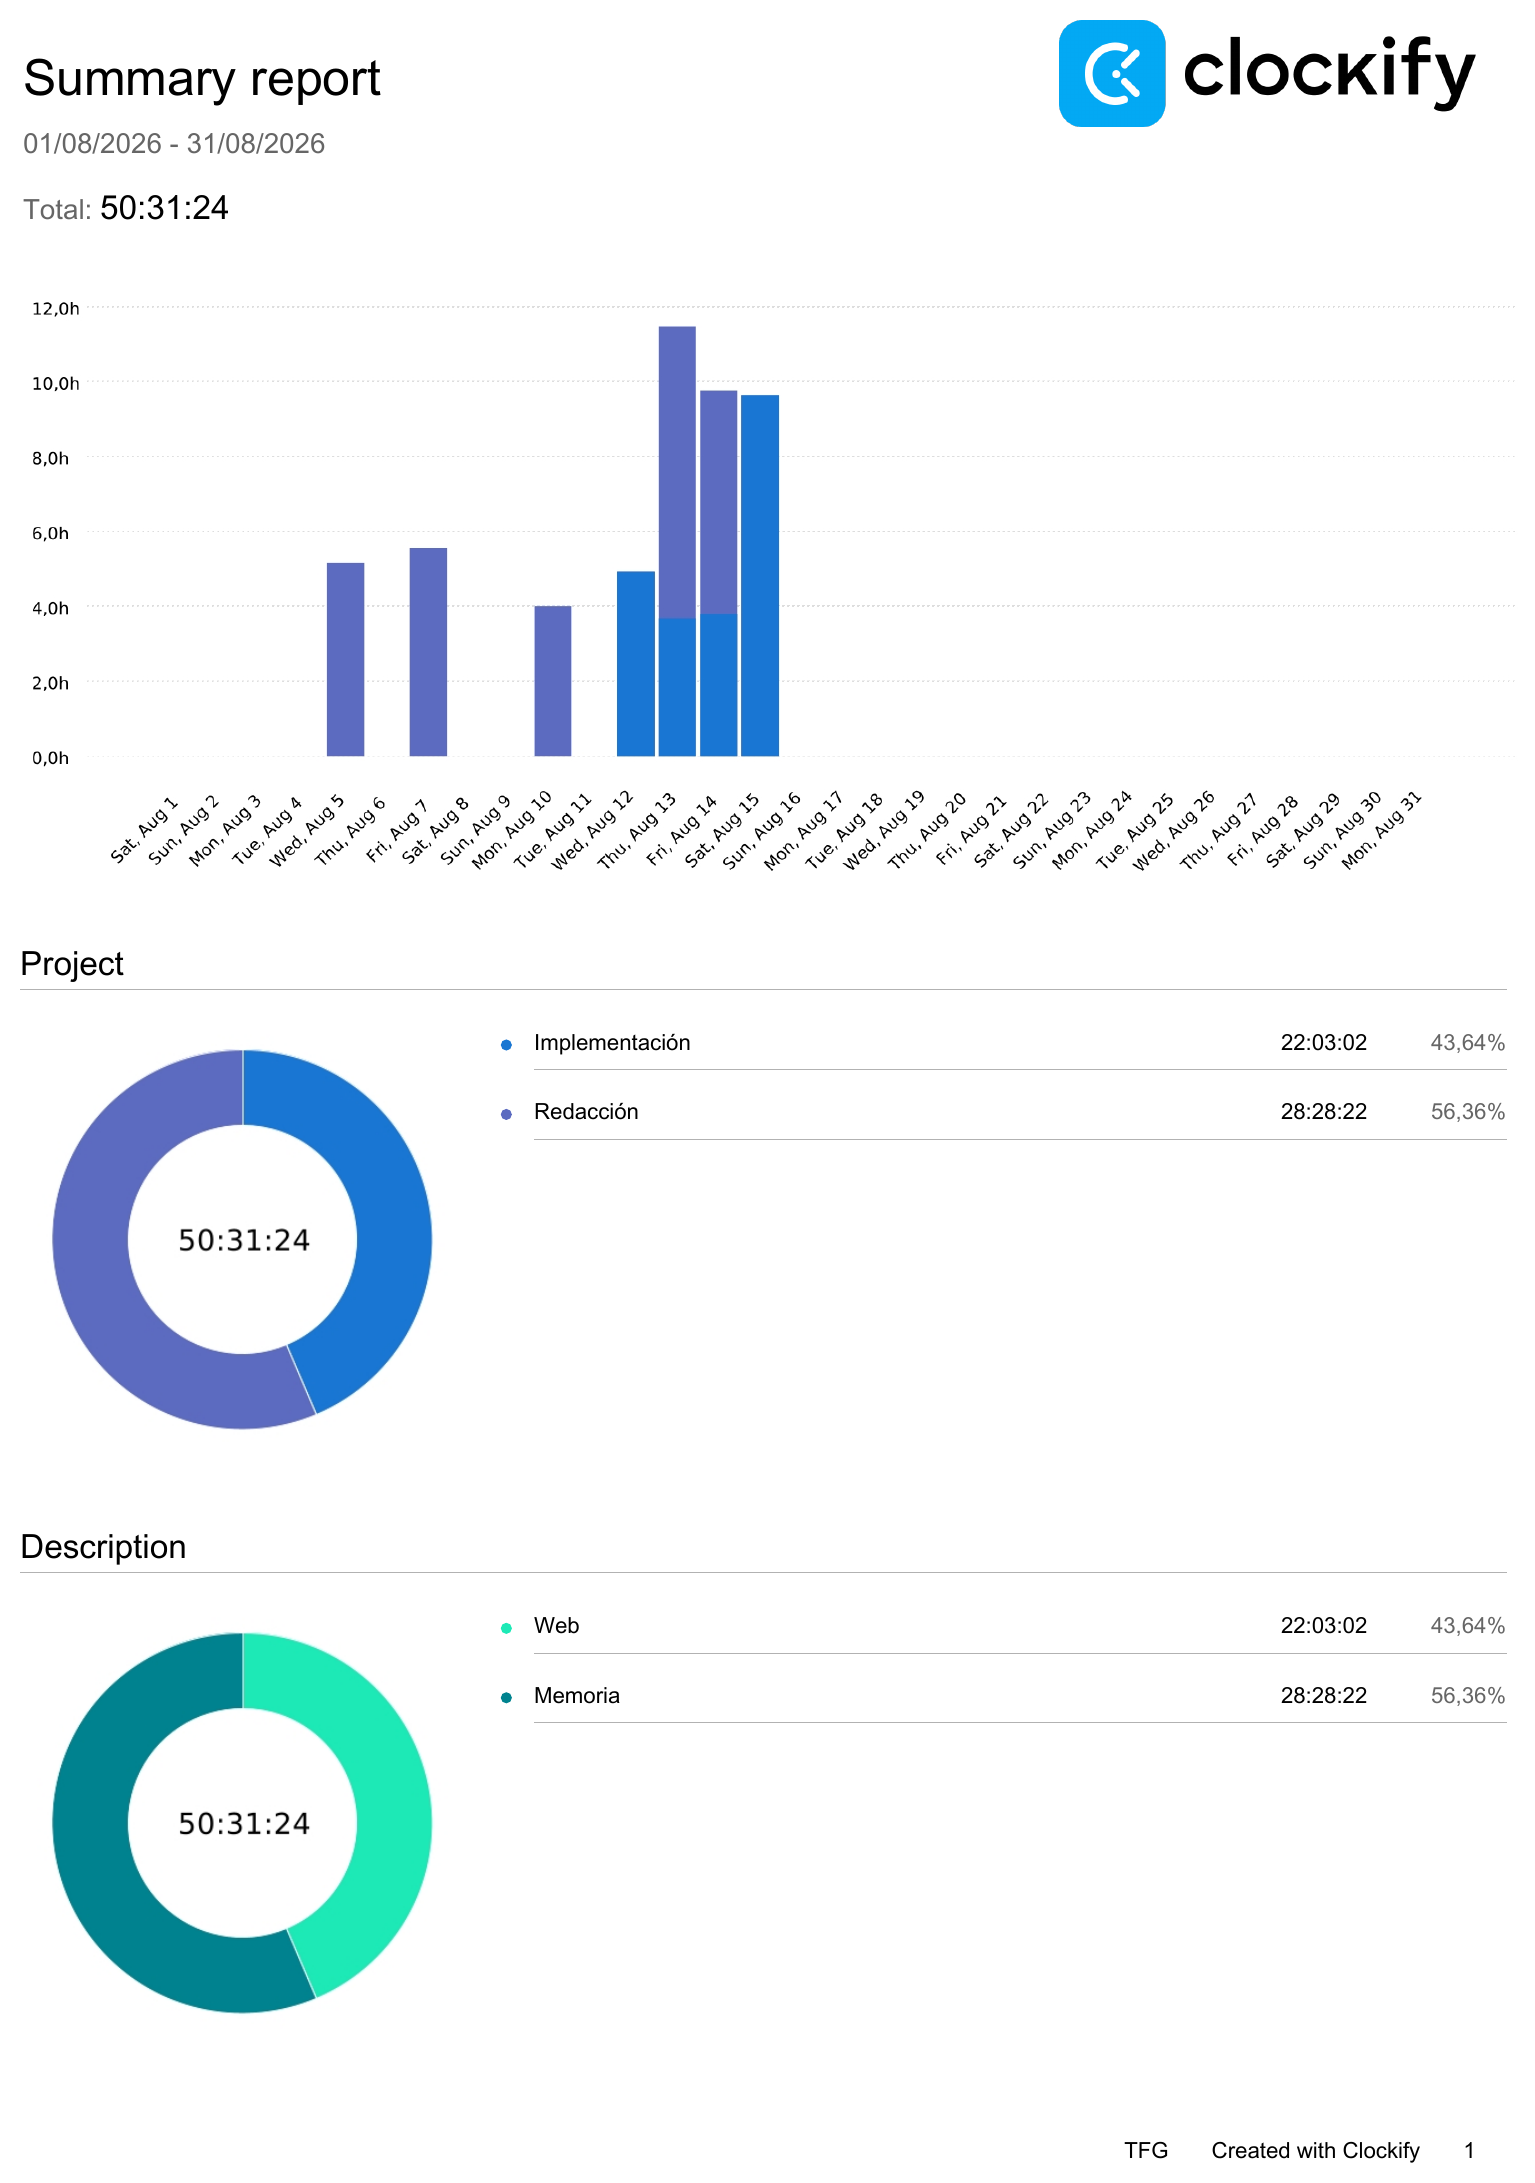
\includegraphics[height=0.72\textheight, keepaspectratio]{figures/clockify_08_2026_p1.png}
\caption{Agosto 2026: unas 51\,h registradas.}
\end{figure}

\FloatBarrier

\begin{figure}[htp]
\centering
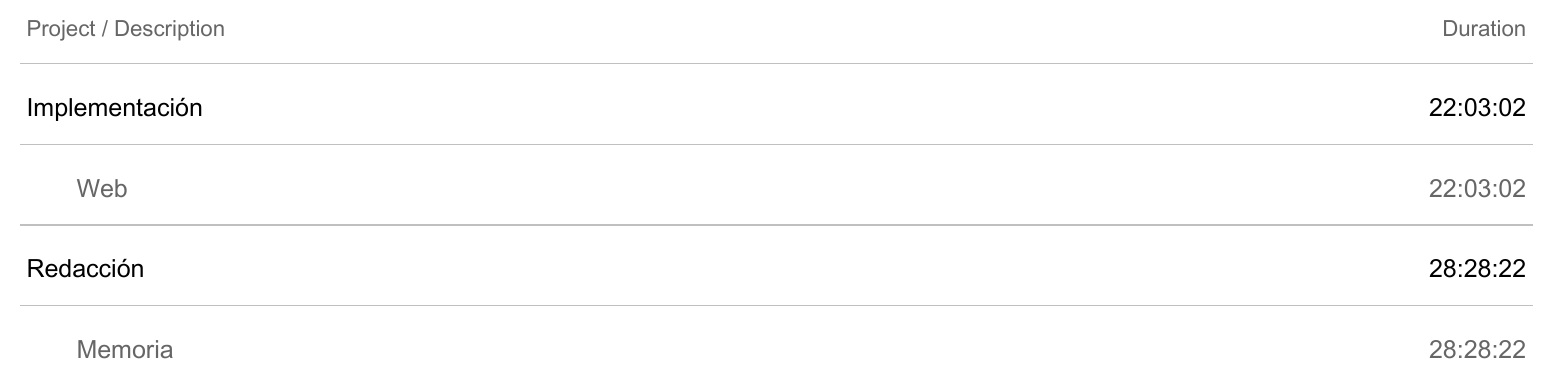
\includegraphics[width=0.92\textwidth, keepaspectratio]{figures/clockify_08_2026_p2.png}
\caption{Agosto 2026: desglose completo de tareas.}
\end{figure}

\FloatBarrier

\begin{figure}[htp]
\centering
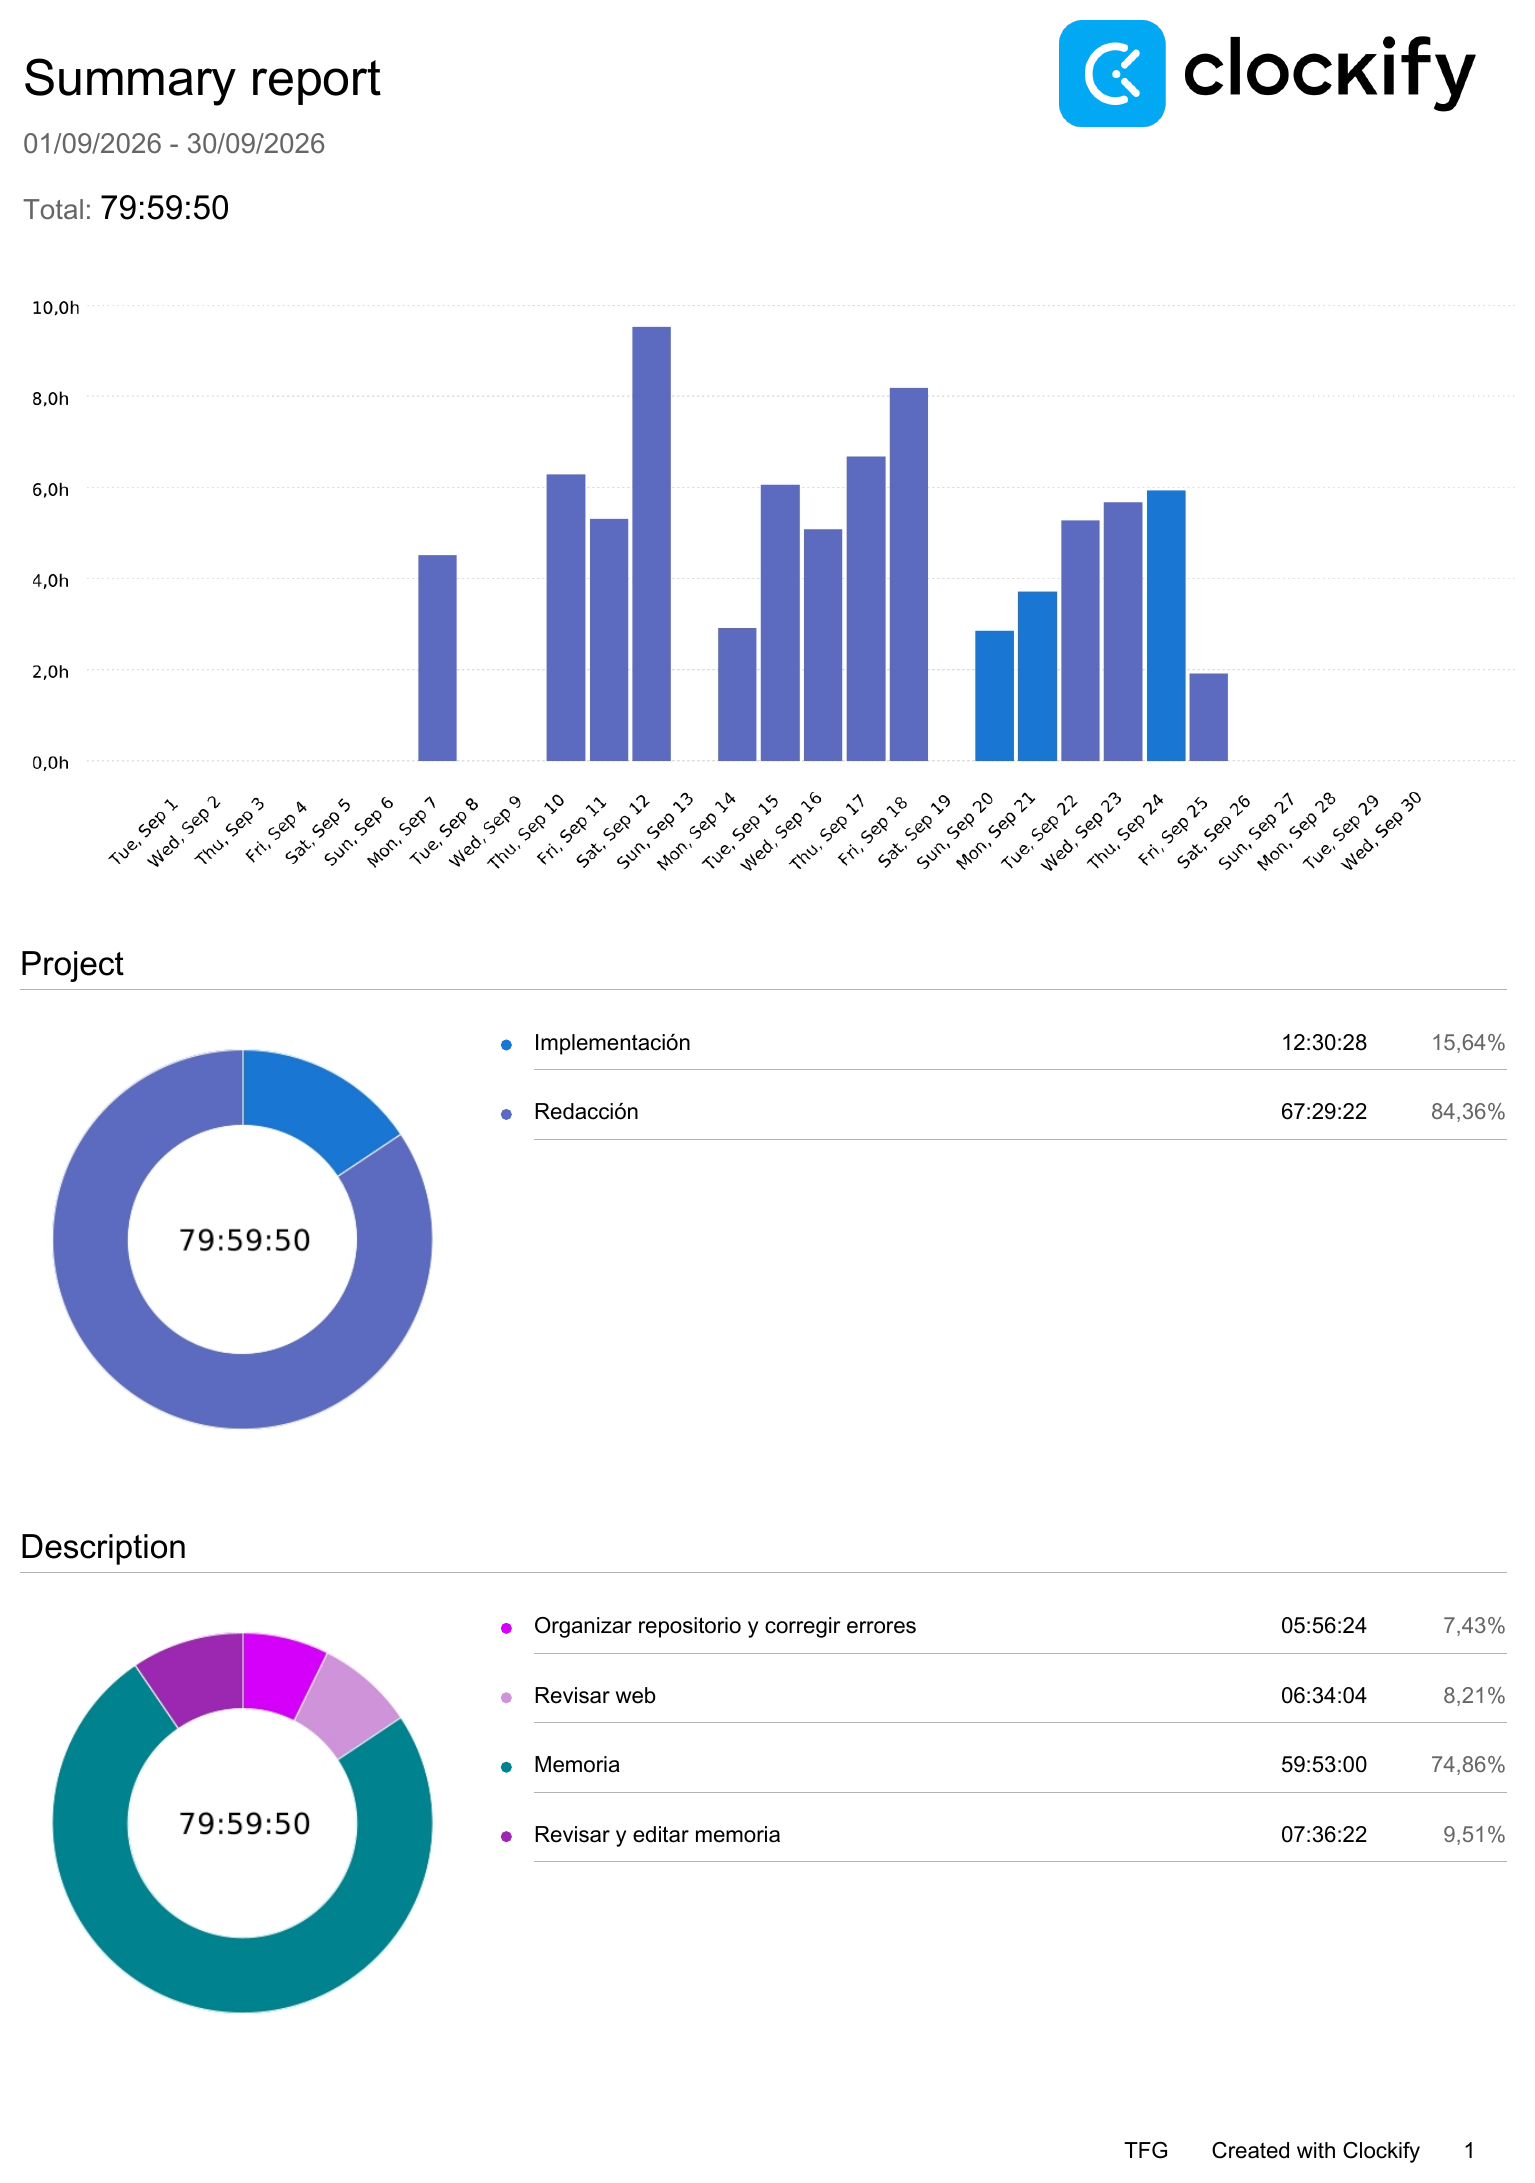
\includegraphics[height=0.72\textheight, keepaspectratio]{figures/clockify_09_2026_p1.png}
\caption{Septiembre 2026: cerca de 80\,h registradas.}
\label{fig:gestion-clockify-sep}
\end{figure}

\FloatBarrier

\begin{figure}[htp]
\centering
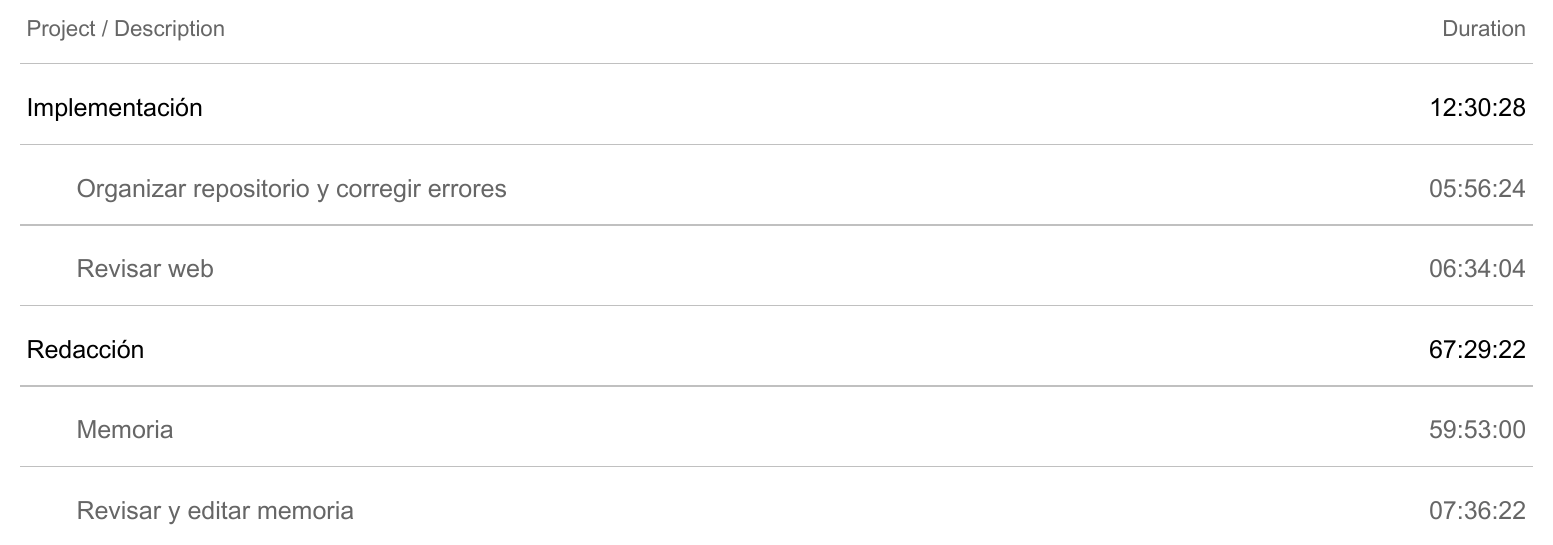
\includegraphics[width=0.92\textwidth, keepaspectratio]{figures/clockify_09_2026_p2.png}
\caption{Septiembre 2026: desglose completo de tareas.}
\label{fig:gestion-clockify-sep-p2}
\end{figure}

\FloatBarrier

\subsection{Hitos principales}

La Tabla~\ref{tab:gestion-hitos} resume los hitos principales alcanzados
hasta el cierre de este documento, reconstruidos a partir del documento de
anotaciones y del historial de commits del repositorio. Las fechas de junio
en adelante son aproximadas, ya que varias tareas se solaparon durante el
desarrollo, como es propio de la metodología iterativa descrita en la
sección~\ref{sec:gestion-metodologia}.

\begin{table}[htp]
\centering
\caption{Hitos principales del proyecto.}
\label{tab:gestion-hitos}
\renewcommand{\arraystretch}{1.3}
\begin{tabular}{|p{2.6cm}|p{9.4cm}|}
\hline
\rowcolor{gray!25}
\textbf{Fecha} & \textbf{Hito} \\
\hline
20--25 abr.\ 2026 & Exploración de tareas de SoccerNet y elección de
  tracking como tarea del proyecto. \\
\hline
26 abr.\ 2026 & OC-SORT y ByteTrack implementados sobre \texttt{boxmot}. \\
\hline
28--29 abr.\ 2026 & \texttt{run\_all\_train.py} ejecutado sobre las 57
  secuencias de train; primera evaluación con TrackEval y exportación de
  vídeos anotados. \\
\hline
Mayo 2026 & Evaluación repetida sobre el conjunto de test a petición del
  tutor; traslado del proyecto a un equipo macOS. \\
\hline
Junio 2026 & Estudio de hiperparámetros de ByteTrack y OC-SORT;
  configuración óptima encontrada para ambos algoritmos. \\
\hline
Junio 2026 & Pipeline de metadatos completo: mapa de calor general,
  clasificación de equipos por color y mapas de calor por equipo,
  homografía real sobre tramos de cámara estable (distancia y velocidad)
  y posesión de balón por proximidad. \\
\hline
Agosto 2026 & Revisión de la planificación, traslado de la entrega a la
  convocatoria de octubre; desarrollo de la aplicación web; grueso de la
  redacción sistemática de la memoria. \\
\hline
Septiembre 2026 & Continuación y grueso final de la redacción de la
  memoria, junto con la organización final del repositorio y una
  revisión de la aplicación web. \\
\hline
Octubre 2026 & Revisión final de la memoria y entrega. \\
\hline
\end{tabular}
\end{table}

\subsection{Revisión de la planificación}
\label{subsec:gestion-revision}

Como es habitual en un proyecto de esta naturaleza, la planificación
inicial no se ha cumplido de forma literal, y merece la pena detenerse en
por qué, ya que las causas de la desviación son en sí mismas informativas
sobre el trabajo realizado. Se identifican cinco causas principales,
ninguna de ellas aislada, sino acumuladas a lo largo del proyecto:

\begin{itemize}
  \item \textbf{Alcance técnico mayor de lo previsto}: el estudio de
        hiperparámetros y el pipeline de metadatos resultaron más
        extensos de lo estimado inicialmente. Cada nuevo metadato
        (clasificación de equipos, mapas de calor, homografía, posesión)
        exigió varias iteraciones de prueba y ajuste antes de dar
        resultados fiables, un coste que la planificación inicial
        (elaborada antes de conocer las dificultades reales de calibrar
        una homografía manual o de separar correctamente al árbitro en la
        clasificación por color) no pudo anticipar.
  \item \textbf{Redacción de la memoria más tardía y más costosa de lo
        previsto}: la planificación inicial contemplaba escribir la
        memoria en paralelo desde junio y cerrarla en julio
        (sección~\ref{sec:gestion-planificacion}). En la práctica, la
        redacción sistemática no arrancó en
        serio hasta agosto, y el grueso del trabajo se concentró entre
        julio y agosto, con continuación y revisión en septiembre y una
        última revisión en octubre. La documentación continua de
        decisiones y resultados intermedios, necesaria para poder
        redactar con este nivel de detalle, ha supuesto por sí misma un
        esfuerzo no contemplado en la planificación inicial.
  \item \textbf{Periodo de exámenes y viajes durante el verano}: además
        del solapamiento ya previsto con los exámenes de mayo, varios periodos de
        viaje durante el verano redujeron la disponibilidad real de
        tiempo en semanas concretas, sin que se hubiera reservado margen
        explícito para ello en la planificación inicial.
  \item \textbf{Retraso inicial por la exploración de alternativas}: la
        fase de exploración inicial de tareas de SoccerNet
         llevó más tiempo del previsto,
        al valorarse varias alternativas antes de comprometerse con el
        tracking como tarea del proyecto
        (sección~\ref{sec:analisis-decision}).
  \item \textbf{Incidencias con el equipo de desarrollo}: un problema con
        el portátil personal con el que se inició el proyecto obligó a
        migrar a un portátil macOS a mitad del desarrollo, en paralelo al
        uso ya habitual de un equipo de sobremesa, y la necesidad de
        recrear el entorno en cada cambio de equipo consumió tiempo no
        planificado.
\end{itemize}

Por este motivo, de acuerdo con el tutor, la entrega del proyecto se ha
trasladado de la convocatoria de julio a la \textbf{convocatoria de
octubre de 2026}, lo que ha permitido completar con mayor profundidad tanto
el pipeline de metadatos como la propia memoria, en lugar de recortar
alcance para cumplir la fecha original. Como consecuencia directa de estas
causas, la dedicación real asciende a las \textbf{313\,h} recogidas en el
diccionario de la EDT (Tabla~\ref{tab:gestion-edt-diccionario}), 13\,h por
encima de las 300\,h de la planificación inicial. La
Tabla~\ref{tab:gestion-desviaciones} resume las principales desviaciones
respecto al plan inicial.

\begin{table}[htp]
\centering
\caption{Principales desviaciones respecto a la planificación inicial.}
\label{tab:gestion-desviaciones}
\renewcommand{\arraystretch}{1.3}
\begin{tabular}{|p{2.6cm}|p{4.6cm}|p{4.8cm}|}
\hline
\rowcolor{gray!25}
\textbf{Elemento} & \textbf{Plan inicial} & \textbf{Desarrollo real} \\
\hline
Estudio de hiperparámetros & Barrido rápido, sin cuantificar horas de
  antemano & Varias iteraciones por algoritmo hasta encontrar una
  configuración óptima defendible \\
\hline
Pipeline de metadatos & Un mapa de calor general & Equipos, heatmaps por
  equipo, homografía (distancia/velocidad) y posesión \\
\hline
Redacción de la memoria & En paralelo desde junio, cerrada en julio &
  Primeros apuntes en junio, arranque real en julio, grueso del trabajo
  en agosto y septiembre, y revisión final en octubre \\
\hline
Aplicación web & Prevista en julio & Desarrollo principal en agosto de
  2026, tras completar el pipeline de metadatos, con un repaso final en
  septiembre (organización del repositorio y revisión de la interfaz) en
  paralelo a la redacción de los últimos capítulos de esta memoria \\
\hline
Horas totales dedicadas & 300\,h (planificación inicial) & 313\,h
  (Tabla~\ref{tab:gestion-edt-diccionario}) \\
\hline
Fecha de entrega & Convocatoria de julio de 2026 & Convocatoria de
  octubre de 2026 \\
\hline
\end{tabular}
\end{table}

\section{Entorno de desarrollo}
\label{sec:gestion-entorno}

El desarrollo se ha realizado en Python 3.11, dentro de un entorno virtual
(\texttt{venv\_tfg}) aislado dentro del propio repositorio del proyecto, con
las dependencias fijadas en \texttt{requirements.txt} para garantizar la
reproducibilidad de los resultados de forma correcta. Las herramientas principales empleadas
son OpenCV (lectura y anotación de frames), \texttt{boxmot} (implementaciones
de los algoritmos de tracking), \texttt{trackeval} (evaluación con métricas
MOT estándar), \texttt{scikit-learn} (clasificación de equipos por color
mediante K-means) y \texttt{matplotlib} (generación de gráficas y mapas de
calor). El desglose completo de versiones y la justificación de las
decisiones técnicas más relevantes sobre el entorno (incluyendo los
problemas encontrados durante su configuración) se detalla en la
sección~\ref{sec:implementacion-entorno} del capítulo~\ref{cap:implementacion}.

El proyecto se inició en un portátil personal HP Pavilion de 8 GB de RAM, y a
mitad del desarrollo se trasladó a un ordenador de sobremesa con GPU AMD
Radeon RX 6900 XT (16\,GB VRAM) como entorno principal. Un problema con el
portátil original obligó, más adelante, a migrar a un portátil macOS,
usado desde entonces en paralelo al equipo de sobremesa según la
disponibilidad; recrear el entorno de desarrollo en cada uno de estos
cambios de equipo (problema P15, sección~\ref{sec:implementacion-entorno})
consumió tiempo no contemplado en la planificación inicial. Dado que
los algoritmos de tracking utilizados en este proyecto (ByteTrack, OC-SORT)
son clásicos y no requieren redes neuronales de gran tamaño en tiempo de
inferencia, todo el desarrollo se ha realizado sobre CPU sin que ello
supusiera una limitación relevante; la GPU AMD, al no ser compatible con
CUDA, se planteó como posible aceleración para líneas de trabajo futuras que
incorporen re-identificación basada en redes neuronales.

\section{Estimación de recursos y presupuesto}
\label{sec:gestion-presupuesto}

Al tratarse de un proyecto académico individual, en este caaso Trabajo Fin de Grado, no ha existido un
presupuesto real asociado a su desarrollo. No obstante, y siguiendo la práctica habitual en
la documentación de proyectos de ingeniería del software, se presenta a continuación una estimación de
los recursos que hubiera requerido su realización en un contexto
profesional, apoyada en los cuatro roles descritos en la
sección~\ref{sec:gestion-roles} y en el diccionario de la EDT de la
sección~\ref{sec:gestion-edt}.

\subsection{Costes de personal}

Las tarifas por hora empleadas en la Tabla~\ref{tab:gestion-costes-personal}
proceden de la \textbf{Instrucción 2/2020, de 30 de junio, de la
Dirección General de Transformación Digital de la Junta de Andalucía,
sobre perfiles y precios de referencia de la contratación de bienes y
servicios TIC} \citep{andalucia2020precios}, que fija precios de
referencia (IVA excluido) para los perfiles profesionales TIC más
comunes según el acuerdo técnico europeo CWA 16458-1:2018. Como esta
instrucción no contempla un perfil específico de \emph{ingeniería de
visión artificial},
se ha usado como equivalente el perfil de \textbf{arquitecto de
sistemas}, el más próximo por nivel de especialización técnica; el resto
de roles de este proyecto sí tienen un perfil directamente equivalente
en la instrucción. La estimación se aplica sobre las horas totales
realmente dedicadas (313\,h, Tabla~\ref{tab:gestion-edt-diccionario}),
repartidas por rol de acuerdo con el diccionario de la EDT.

\begin{table}[htp]
\centering
\caption{Estimación de costes de personal sobre las 313\,h reales dedicadas al proyecto.}
\label{tab:gestion-costes-personal}
\renewcommand{\arraystretch}{1.3}
\begin{tabular}{|p{3.6cm}|p{3.4cm}|r|r|r|}
\hline
\rowcolor{gray!25}
\textbf{Rol} & \textbf{Perfil equivalente (Junta de Andalucía)} & \textbf{Horas} & \textbf{€/h} & \textbf{Coste} \\
\hline
Jefe de proyecto & Gestor de proyecto & 90\,h & 44{,}12\,€ & 3\,970{,}80\,€ \\
\hline
Analista de software & Analista de negocio & 15\,h & 33{,}17\,€ & 497{,}55\,€ \\
\hline
Ingeniero de Visión Artificial & Arquitecto de sistemas & 143\,h & 33{,}45\,€ & 4\,783{,}35\,€ \\
\hline
Desarrollador & Desarrollador & 65\,h & 25{,}67\,€ & 1\,668{,}55\,€ \\
\hline
\rowcolor{gray!10}
\textbf{Total} & & \textbf{313\,h} & & \textbf{10\,920{,}25\,€} \\
\hline
\end{tabular}
\end{table}

\subsection{Costes materiales y operacionales}

Además de los costes de personal, un proyecto de estas características
conllevaría los costes materiales y operacionales que recoge la
Tabla~\ref{tab:gestion-costes-operacionales}. La mayoría son recursos sin
coste directo, por tratarse de equipo ya disponible o de herramientas de
código abierto; el único coste realmente cuantificable es el consumo
eléctrico, calculado a partir de una potencia media de consumo de
150\,W, una cifra intermedia entre el portátil y el equipo de sobremesa
descritos en la sección~\ref{sec:gestion-entorno}, ya que no todas las
313\,h de dedicación se han realizado con el equipo de mayor consumo y
las 313\,h totales del proyecto (Tabla~\ref{tab:gestion-edt-diccionario}):
$150\,\mathrm{W} \times 313\,\mathrm{h} = 46{,}95\,\mathrm{kWh}$, que al precio
medio doméstico de la electricidad en España (en torno a 0{,}16\,€/kWh)
supone un coste estimado de \textbf{7{,}51\,€} a lo largo de todo el
proyecto.

\begin{table}[htp]
\centering
\caption{Costes materiales y operacionales estimados.}
\label{tab:gestion-costes-operacionales}
\renewcommand{\arraystretch}{1.3}
\begin{tabular}{|p{5.4cm}|p{6.4cm}|}
\hline
\rowcolor{gray!25}
\textbf{Concepto} & \textbf{Coste} \\
\hline
Hardware (equipo de desarrollo ya disponible, sin GPU dedicada necesaria,
  sección~\ref{sec:gestion-entorno}) & Sin coste incremental \\
\hline
Software y librerías (Python, OpenCV, \texttt{boxmot}, \texttt{trackeval},
  scikit-learn, matplotlib, Git) & 0\,€ (código abierto) \\
\hline
Dataset (SoccerNet-Tracking) & 0\,€ (acceso académico gratuito) \\
\hline
Asistentes de inteligencia artificial (Claude Code,
  capítulo~\ref{cap:uso-ia}) & No cuantificado en esta estimación \\
\hline
Consumo eléctrico ($150\,\mathrm{W} \times 313\,\mathrm{h} = 46{,}95\,\mathrm{kWh}$
  a 0{,}16\,€/kWh) & 7{,}51\,€ \\
\hline
\rowcolor{gray!10}
\textbf{Total cuantificado} & \textbf{7{,}51\,€} \\
\hline
\end{tabular}
\end{table}

Este bajo coste de infraestructura es, precisamente, uno de los factores que
hace atractivo el enfoque seguido en este proyecto (véase la justificación de
la elección de tarea en la sección~\ref{sec:analisis-decision}): al partir de
detecciones ya calculadas y de algoritmos de tracking clásicos disponibles
como librería, el proyecto es reproducible por terceros sin inversión en
infraestructura específica.

\subsection{Desviación respecto al coste planificado}

Como se describe en la sección~\ref{subsec:gestion-revision}, la dedicación
real (313\,h) ha superado en 13\,h la planificación inicial de 300\,h,
principalmente por el mayor alcance del estudio de hiperparámetros y del
pipeline de metadatos, y por el tiempo dedicado a documentar el proceso
con el nivel de detalle de esta memoria. A diferencia de lo que ocurriría
sin un registro fiable de horas, en este proyecto sí se ha dispuesto de
una herramienta de \emph{time-tracking} dedicada
(sección~\ref{subsec:gestion-monitorizacion}), lo que permite ofrecer una
cifra de coste real y no solo una desviación cualitativa: aplicando las
mismas tarifas de la Tabla~\ref{tab:gestion-costes-personal} sobre el
reparto por rol de las 300\,h de la planificación inicial (40\,h jefe de
proyecto, 20\,h analista, 165\,h ingeniero de Visión Artificial, 75\,h
desarrollador) y el mismo criterio de consumo eléctrico sobre esas 300\,h
($150\,\mathrm{W} \times 300\,\mathrm{h} = 45\,\mathrm{kWh}$, a
0{,}16\,€/kWh), se obtiene el coste total estimado que recoge la
Tabla~\ref{tab:gestion-costes-resumen}, comparado con el coste real
final.

\begin{table}[htp]
\centering
\caption{Coste total estimado frente a coste real y desviación.}
\label{tab:gestion-costes-resumen}
\renewcommand{\arraystretch}{1.3}
\begin{tabular}{|p{3.6cm}|r|r|r|}
\hline
\rowcolor{gray!25}
\textbf{Concepto} & \textbf{Coste estimado} & \textbf{Coste real} & \textbf{Desviación} \\
\hline
Personal (Tabla~\ref{tab:gestion-costes-personal}) & 9\,872{,}70\,€ &
  10\,920{,}25\,€ & +1\,047{,}55\,€ \\
\hline
Consumo eléctrico (Tabla~\ref{tab:gestion-costes-operacionales}) &
  7{,}20\,€ & 7{,}51\,€ & +0{,}31\,€ \\
\hline
\rowcolor{gray!10}
\textbf{Total} & \textbf{9\,879{,}90\,€} & \textbf{10\,927{,}76\,€} &
  \textbf{+1\,047{,}86\,€ (+10{,}6\,\%)} \\
\hline
\end{tabular}
\end{table}

La desviación de coste total, en torno al 10{,}6\,\%, es mayor que la
desviación de horas (13\,h sobre 300\,h, un 4{,}3\,\%) porque el exceso
de horas se concentra casi en su totalidad en el rol de tarifa más alta,
el jefe de proyecto (90\,h reales frente a 40\,h planificadas), mientras
que el resto de roles se ha mantenido por debajo de lo previsto; el
consumo eléctrico, al ser proporcional a las horas totales, se desvía en
una proporción prácticamente idéntica a la de las horas (4{,}3\,\%) pero
su magnitud absoluta es tan pequeña que apenas afecta al total. La
Tabla~\ref{tab:gestion-desviaciones} documenta
el resto de desviaciones respecto a la planificación inicial, no solo la
de coste.

\section{Plan de gestión de riesgos}
\label{sec:gestion-riesgos}

La gestión de riesgos de este proyecto no se ha limitado a una lista
elaborada una única vez al inicio, sino que se ha
revisado en cada feedback de seguimiento con el tutor, incorporando riesgos
nuevos a medida que se hacían evidentes. Por ejemplo, el riesgo asociado a
la dependencia de \texttt{boxmot} no era previsible hasta que la propia
librería cambió de interfaz durante el desarrollo del proyecto. Para
cada riesgo se ha estimado su probabilidad e impacto de forma cualitativa
(alta/media/baja), se han definido medidas preventivas aplicadas durante el
desarrollo. La Tabla~\ref{tab:gestion-riesgos-tabla} recoge los cinco
riesgos principales identificados durante la planificación y el
desarrollo del proyecto.

\begin{table}[htp]
\centering
\caption{Principales riesgos del proyecto y su mitigación.}
\label{tab:gestion-riesgos-tabla}
\renewcommand{\arraystretch}{1.3}
\begin{tabular}{|p{3.0cm}|p{4.5cm}|p{4.5cm}|}
\hline
\rowcolor{gray!25}
\textbf{Riesgo} & \textbf{Medidas preventivas} & \textbf{Plan de contingencia} \\
\hline
Disponibilidad de tiempo irregular por exámenes &
  Margen amplio en la planificación inicial (aprox.\ 65\,h de colchón) &
  Traslado de la entrega a la convocatoria de octubre. \\
\hline
Dependencia de \texttt{boxmot}, librería en evolución activa con cambios de
  interfaz entre versiones &
  Versión antigua fijada en \texttt{requirements.txt} y código
  versionado en Git (problema P4, sección~\ref{sec:implementacion-entorno}) &
  Congelar la versión funcional y documentar el problema en vez de migrar
  a mitad de proyecto \\
\hline
Resultados de calibración de cámara no generalizables a todo el dataset &
  Acotar expresamente la homografía real a una prueba de concepto sobre
  tramos con cámara estable &
  Documentar la limitación en la memoria en vez de invertir tiempo buscar otras formas. \\
\hline
Cambio de equipo de desarrollo a mitad de proyecto (traslado a macOS) &
  Dependencias fijadas en \texttt{requirements.txt} y código versionado
  en Git &
  Recrear el entorno desde cero en el nuevo equipo (problema P15,
  sección~\ref{sec:implementacion-entorno}) \\
\hline
Redacción de la memoria más tardía y más costosa de lo previsto &
  Documento de anotaciones actualizado de forma continua durante todo el
  desarrollo (sección~\ref{sec:gestion-metodologia}), que evita depender
  de la memoria para no perder el registro de decisiones &
  Traslado de la entrega a la convocatoria de octubre y redacción en
  paralelo a las últimas iteraciones técnicas. \\
\hline
\end{tabular}
\end{table}

\section{Plan de calidad}
\label{sec:gestion-calidad}

La calidad de este proyecto no se ha evaluado únicamente por si el código
se ejecuta sin errores, sino por un conjunto más amplio de criterios
propios de un proyecto de análisis de datos: que los resultados de
tracking sean válidos y evaluables con herramientas estándar, que la
comparación entre algoritmos y configuraciones sea reproducible, que cada
metadato extraído documente explícitamente sus limitaciones en lugar de
presentarse como una medida exacta, y que el conjunto del proceso quede
justificado por escrito. La Tabla~\ref{tab:gestion-calidad} resume los
criterios de calidad aplicados en cada área del proyecto y cómo se ha
comprobado su cumplimiento.

\begin{table}[htp]
\centering
\caption{Plan de calidad del proyecto.}
\label{tab:gestion-calidad}
\renewcommand{\arraystretch}{1.05}
\footnotesize
\begin{tabular}{|p{2.6cm}|p{4.5cm}|p{4.9cm}|}
\hline
\rowcolor{gray!25}
\textbf{Área} & \textbf{Criterio de calidad} & \textbf{Comprobación} \\
\hline
Resultados de tracking & Formato MOT válido y coherente con
  \texttt{trackeval} & Ejecución de TrackEval sin errores sobre todas las
  secuencias de train y test \\
\hline
Evaluación & Comparación de algoritmos con métricas estándar
  (HOTA, MOTA, IDF1) & Revisión cruzada de los CSV/gráficas generados por
  TrackEval \\
\hline
Hiperparámetros & Barrido reproducible, un parámetro a la vez sobre el
  mismo split & Configuración óptima verificada con una segunda ejecución
  independiente (\texttt{*\_optimal.py}) \\
\hline
Metadatos & Cada metadato documenta explícitamente su limitación (balón,
  árbitro, homografía parcial) & Revisión visual de las figuras generadas
  frente a los datos crudos \\
\hline
Reproducibilidad & Entorno fijado en \texttt{requirements.txt}, resultados
  intermedios persistidos en disco & Recreación del entorno en dos equipos
  distintos (sobremesa Windows y macOS) sin incidencias relevantes \\
\hline
Documentación & Cada decisión técnica queda justificada en la memoria &
  Contraste sistemático de las anotaciones propias con el código real del
  repositorio (véase capítulo~\ref{cap:uso-ia}) \\
\hline
Anomalías & Las trayectorias con saltos de posición incompatibles con un
  movimiento humano real se detectan y excluyen en vez de aceptarse sin
  más & Revisión visual de las trayectorias proyectadas por homografía;
  exclusión manual documentada de los \emph{track\_id} anómalos
  (sección~\ref{sec:implementacion-homografia}) \\
\hline
Explicabilidad de las predicciones & Cada resultado del pipeline es
  trazable a una regla o un parámetro explícito, no a un modelo de caja
  negra & Revisión manual de casos concretos (p.\ ej., por qué una
  detección se clasifica como balón o a qué equipo se asigna un jugador)
  contra los umbrales exactos documentados en el
  capítulo~\ref{cap:implementacion} \\
\hline
Código & Organización en paquetes por responsabilidad, sin lógica
  duplicada entre scripts & Revisión de la estructura del repositorio
  (Tabla~\ref{tab:impl-estructura}); reutilización explícita de la
  lógica de \texttt{src/metadata/} desde \texttt{src/web\_export/} en vez
  de duplicarla \\
\hline
Optimización & Los artefactos generados no consumen más recursos de los
  necesarios (tiempo de cómputo, tamaño en disco) & Muestreo de
  1 de cada 5 \emph{frames} en la clasificación de equipos
  (sección~\ref{subsec:impl-equipos}); elección del \emph{fourcc}
  \texttt{avc1} para los vídeos de la web, que redujo su tamaño en torno
  a un 75\,\% (sección~\ref{subsec:impl-web-bundle}) \\
\hline
Aplicación web & Interfaz funcional fiel al diseño planificado, sin
  necesidad de \emph{backend} & Verificación manual de ambas pestañas con
  datos reales; \texttt{npm run build} sin errores y sitio servido en
  local con \texttt{npm run preview} (sección~\ref{sec:manual-web}) \\
\hline
\end{tabular}
\end{table}

    \chapter{Análisis de requisitos}
\label{cap:analisis}

Este capítulo describe el análisis funcional del sistema desarrollado en
este proyecto, en el capítulo se describen: los actores que interactúan con él, los requisitos de
información, los requisitos funcionales y no
funcionales que debe satisfacer, las reglas de negocio, y los casos de uso que formalizan cómo se usa. 
Finalmente el capítulo
se cierra con una matriz de trazabilidad que relaciona cada requisito con
los objetivos específicos definidos en la
sección~\ref{sec:intro-objetivos} del capítulo~\ref{cap:introduccion},
de modo que pueda comprobarse que ningún objetivo queda sin cubrir y que
ningún requisito queda fuera de los fines del proyecto.

\section{Contexto funcional del sistema}
\label{sec:analisis-contexto}

El sistema desarrollado en este proyecto aborda la comparación de
algoritmos de seguimiento multiobjeto sobre vídeo de fútbol y la extracción
de metadatos deportivos a partir de las trayectorias resultantes. Se
organiza en dos bloques con una naturaleza muy distinta, representados en
la Figura~\ref{fig:analisis-contexto}: un \textbf{pipeline offline} en
Python, que concentra todo el cómputo pesado, y una
\textbf{aplicación web} de visualización (sección~\ref{sec:implementacion-web}),
que consume los resultados ya calculados por el pipeline. El planteamiento se detalla en el
capítulo~\ref{cap:diseno}.

\begin{figure}[htp]
\centering
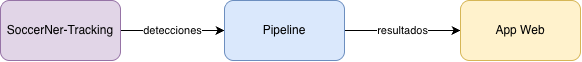
\includegraphics[width=0.7\textwidth]{figures/contexto_funcional.drawio.png}
\caption{Contexto funcional del sistema: el dataset público como entrada, el
pipeline offline como bloque de cómputo, y la aplicación web como capa de
visualización sobre los resultados.}
\label{fig:analisis-contexto}
\end{figure}

\subsection{Justificación y decisión de la tarea elegida}
\label{sec:analisis-decision}

Antes de comprometerse con el seguimiento multiobjeto como tarea de este
proyecto, se exploraron brevemente otras tareas del ecosistema SoccerNet, como parte de la primera fase del
proyecto descrita en la sección~\ref{sec:gestion-fases}. Concretamente, se
valoraron tres alternativas:

\begin{itemize}
  \item \textbf{Reconocimiento de dorsales} (\emph{jersey number
        recognition}): predecir el número de un jugador a partir de una
        imagen recortada. Se consideró una opción técnicamente válida y de
        alta viabilidad que era adecuada para el contexto del proyecto, ya
        que trataba de trabajar sobre imágenes estáticas, no sobre
        secuencias, pero con menor profundidad técnica para una
        comparativa de algoritmos, el enfoque que finalmente se decidió dar
        a este proyecto.
  \item \textbf{Segmentación de cámara} (\emph{camera segmentation}):
        clasificar en cada instante del vídeo el tipo de plano de cámara
        (plano general, primer plano, repetición). Se descartó sin llegar a
        explorarse ni implementarse: se valoró como menos interesante
        técnicamente y de menor impacto visual en una demostración que las
        otras dos alternativas.
  \item \textbf{Seguimiento multiobjeto} (MOT, sección~\ref{sec:fundamentos-mot}):
        la tarea finalmente elegida.
\end{itemize}

La decisión final se apoyó en varios factores concretos, verificados
mediante pruebas exploratorias reales antes de comprometerse con la tarea:
el dataset SoccerNet-Tracking incluye detecciones ya calculadas, lo
que elimina la barrera de tener que entrenar o adaptar un detector de
objetos propio; en apenas unas horas de exploración inicial fue posible
pasar de cero a visualizaciones funcionales sobre el \emph{ground truth}; el
tutor confirmó que era válido plantear el trabajo como una comparativa
rigurosa de varios algoritmos de \emph{tracking-by-detection}
(sección~\ref{sec:fundamentos-algoritmos}), en lugar de limitarse a
implementar uno solo; y la posibilidad de una demostración web con mapa de
calor de trayectorias se valoró como la más atractiva visualmente de las
tres alternativas exploradas.

Como consecuencia directa de esta decisión, y como se ha detallado en la
sección~\ref{sec:fundamentos-algoritmos}, se seleccionó la librería
\texttt{boxmot}, la cual agrupa varias implementaciones de algoritmos de
tracking bajo una interfaz común, de modo que cambiar de algoritmo se
reduce a cambiar una línea de código, ideal para una comparativa, fijando
específicamente su versión \texttt{10.0.43}, ya que versiones posteriores
de la librería (a partir de la v18) dejaron de mostrar las clases de cada
algoritmo por separado, unificándolas bajo una única interfaz, lo cual no se
quería en este proyecto, ya que dificultaba precisamente la comparación que el proyecto
necesitaba. Para la evaluación se adoptó \texttt{TrackEval}, por ser la herramienta de
referencia oficial del propio benchmark de SoccerNet y que funciona muy bien con el formato MOT estándar que produce \texttt{boxmot}.

\section{Actores y usuarios del sistema}
\label{sec:analisis-actores}

La aplicación web, una vez
desarrollada, consumirá artefactos estáticos sin sesión de usuario. Por
ese motivo, los actores no son usuarios con inicio de sesión, sino roles o
perspectivas de uso frente al sistema. En el desarrollo, es solo el autor del proyecto quien
asume los roles internos, pero
se describen por separado porque responden a objetivos distintos frente al
sistema, del mismo modo que se distinguieron los roles de gestión en la
sección~\ref{sec:gestion-roles}.

Se identifican dos actores primarios y un actor secundario, representados
en la Figura~\ref{fig:analisis-actores} y descritos en la
Tabla~\ref{tab:analisis-actores}: el \textbf{operador del pipeline}, que
ejecuta las distintas fases del procesamiento offline, el \textbf{usuario
analista} que consulta la aplicación web para explorar e interpretar los
resultados y SoccerNet, como sistema externo del
que el pipeline obtiene los datos de entrada.

\begin{figure}[htp]
\centering
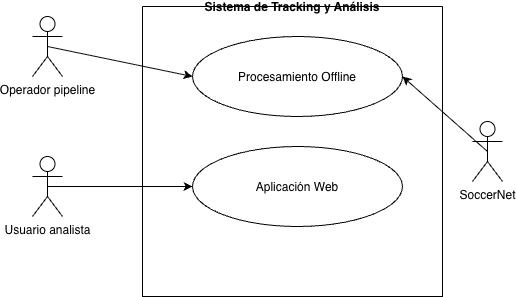
\includegraphics[width=0.7\textwidth]{figures/diagrama_actores.drawio.png}
\caption{Actores del sistema: operador del pipeline y usuario analista
(izquierda), interactuando respectivamente con el procesamiento offline y
la aplicación web, y SoccerNet como sistema externo (derecha).}
\label{fig:analisis-actores}
\end{figure}

\begin{table}[htp]
\centering
\caption{Actores y usuarios del sistema.}
\label{tab:analisis-actores}
\renewcommand{\arraystretch}{1.3}
\begin{tabular}{|p{2.7cm}|p{1.7cm}|p{7.9cm}|}
\hline
\rowcolor{gray!25}
\textbf{Actor} & \textbf{Tipo} & \textbf{Descripción} \\
\hline
Operador del pipeline & Primario &
  Ejecuta las fases del procesamiento offline: descarga del dataset,
  tracking, evaluación, estudio de hiperparámetros y extracción de
  metadatos. \\
\hline
Usuario analista & Primario &
  Consulta la aplicación web para explorar los vídeos
  anotados, las métricas comparativas y los metadatos deportivos
  generados. \\
\hline
SoccerNet & Secundario &
  Sistema externo del que se obtienen las secuencias de vídeo, las
  detecciones precomputadas y el \emph{ground truth}
  (sección~\ref{subsec:fundamentos-soccernet-tracking}). \\
\hline
\end{tabular}
\end{table}

\section{Requisitos de información}
\label{sec:analisis-irq}

Los requisitos de información indican qué datos debe recopilar, generar y
conservar el sistema para ejecutar el pipeline. Se recogen en las Tablas~\ref{tab:irq-001}
a~\ref{tab:irq-009}.

\begin{table}[htp]
\centering
\caption{IRQ-001: Detecciones precomputadas de SoccerNet-Tracking.}
\label{tab:irq-001}
\renewcommand{\arraystretch}{1.2}
\begin{tabular}{|p{3.1cm}|p{9.2cm}|}
\hline
\rowcolor{gray!25}
\multicolumn{2}{|l|}{\textbf{IRQ-001 -- Detecciones precomputadas de SoccerNet-Tracking}} \\
\hline
Versión & v1.0 \\
\hline
Rol & Operador del pipeline \\
\hline
Datos específicos & \texttt{frame\_id}, \texttt{x}, \texttt{y}, \texttt{w},
  \texttt{h}, \texttt{confianza} (fichero \texttt{det.txt} por secuencia) \\
\hline
Descripción & El sistema debe leer, para cada secuencia, las detecciones ya
  calculadas de jugadores, árbitros y balón, como entrada de los
  algoritmos de tracking (sección~\ref{sec:fundamentos-mot}). \\
\hline
\end{tabular}
\end{table}

\begin{table}[htp]
\centering
\caption{IRQ-002: \emph{Ground truth} de tracking.}
\label{tab:irq-002}
\renewcommand{\arraystretch}{1.2}
\begin{tabular}{|p{3.1cm}|p{9.2cm}|}
\hline
\rowcolor{gray!25}
\multicolumn{2}{|l|}{\textbf{IRQ-002 -- \emph{Ground truth} de tracking}} \\
\hline
Versión & v1.0 \\
\hline
Rol & Operador del pipeline \\
\hline
Datos específicos & \texttt{frame\_id}, \texttt{obj\_id}, \texttt{x},
  \texttt{y}, \texttt{w}, \texttt{h} (fichero \texttt{gt.txt}, solo en
  train y test) \\
\hline
Descripción & El sistema debe leer la posición e identidad real de cada
  objeto por frame, como referencia para calcular las métricas de
  evaluación (sección~\ref{sec:fundamentos-metricas}). \\
\hline
\end{tabular}
\end{table}

\begin{table}[htp]
\centering
\caption{IRQ-003: Metadatos de secuencia y de partido.}
\label{tab:irq-003}
\renewcommand{\arraystretch}{1.2}
\begin{tabular}{|p{3.1cm}|p{9.2cm}|}
\hline
\rowcolor{gray!25}
\multicolumn{2}{|l|}{\textbf{IRQ-003 -- Metadatos de secuencia y de partido}} \\
\hline
Versión & v1.0 \\
\hline
Rol & Operador del pipeline \\
\hline
Datos específicos & Resolución de imagen y \emph{frame rate}
  (\texttt{seqinfo.ini}); \\
\hline
Descripción & El sistema debe conservar esta información de contexto de
  cada secuencia, necesaria para interpretar correctamente sus detecciones
  y para la configuración de \texttt{TrackEval}. \\
\hline
\end{tabular}
\end{table}

\begin{table}[htp]
\centering
\caption{IRQ-004: Resultados de tracking por algoritmo.}
\label{tab:irq-004}
\renewcommand{\arraystretch}{1.2}
\begin{tabular}{|p{3.1cm}|p{9.2cm}|}
\hline
\rowcolor{gray!25}
\multicolumn{2}{|l|}{\textbf{IRQ-004 -- Resultados de tracking por algoritmo}} \\
\hline
Versión & v1.0 \\
\hline
Rol & Operador del pipeline \\
\hline
Datos específicos & \texttt{frame,id,x,y,w,h,conf,-1,-1,-1} (formato MOT),
  un fichero \texttt{.txt} por secuencia y algoritmo, en
  \texttt{results\_train/}, \texttt{results\_test/} y
  \texttt{results\_hyperparam/} \\
\hline
Descripción & El sistema debe persistir las trayectorias resultantes de
  cada algoritmo de tracking sobre cada secuencia, en el formato estándar
  que consume \texttt{TrackEval}. \\
\hline
\end{tabular}
\end{table}

\begin{table}[htp]
\centering
\caption{IRQ-005: Resultados de evaluación con métricas MOT.}
\label{tab:irq-005}
\renewcommand{\arraystretch}{1.2}
\begin{tabular}{|p{3.1cm}|p{9.2cm}|}
\hline
\rowcolor{gray!25}
\multicolumn{2}{|l|}{\textbf{IRQ-005 -- Resultados de evaluación con métricas MOT}} \\
\hline
Versión & v1.0 \\
\hline
Rol & Operador del pipeline \\
\hline
Datos específicos & HOTA, HOTA(0), DetA, AssA, MOTA, IDF1, IDSW por
  secuencia y combinado \\
\hline
Descripción & El sistema debe conservar las métricas calculadas por
  \texttt{TrackEval} para cada algoritmo, tanto por secuencia como
  combinadas, como base del análisis comparativo del
  capítulo~\ref{cap:pruebas}. \\
\hline
\end{tabular}
\end{table}

\begin{table}[htp]
\centering
\caption{IRQ-006: Resultados del estudio de hiperparámetros.}
\label{tab:irq-006}
\renewcommand{\arraystretch}{1.2}
\begin{tabular}{|p{3.1cm}|p{9.2cm}|}
\hline
\rowcolor{gray!25}
\multicolumn{2}{|l|}{\textbf{IRQ-006 -- Resultados del estudio de hiperparámetros}} \\
\hline
Versión & v1.0 \\
\hline
Rol & Operador del pipeline \\
\hline
Datos específicos & \texttt{algo, tracker, param, value, HOTA, MOTA, IDF1,
  IDSW} (\texttt{summary\_table.csv} y gráficas en
  \texttt{evaluation\_hyperparam/}) \\
\hline
Descripción & El sistema debe conservar, para cada valor probado de cada
  hiperparámetro, las métricas resultantes, con el fin de justificar la
  configuración óptima seleccionada. \\
\hline
\end{tabular}
\end{table}

\begin{table}[htp]
\centering
\caption{IRQ-007: Clasificación de jugadores por equipo.}
\label{tab:irq-007}
\renewcommand{\arraystretch}{1.2}
\begin{tabular}{|p{3.1cm}|p{9.2cm}|}
\hline
\rowcolor{gray!25}
\multicolumn{2}{|l|}{\textbf{IRQ-007 -- Clasificación de jugadores por equipo}} \\
\hline
Versión & v1.0 \\
\hline
Rol & Operador del pipeline \\
\hline
Datos específicos & \texttt{frame, track\_id, team, b, g, r} y
  \texttt{track\_id, team}, en
  \texttt{metadata\_output/teams/} \\
\hline
Descripción & El sistema debe conservar la asignación de cada jugador a un
  equipo (0 o 1), obtenida mediante K-means sobre el color de camiseta
  (sección~\ref{sec:fundamentos-kmeans}). \\
\hline
\end{tabular}
\end{table}

\begin{table}[htp]
\centering
\caption{IRQ-008: Metadatos deportivos derivados.}
\label{tab:irq-008}
\renewcommand{\arraystretch}{1.2}
\begin{tabular}{|p{3.1cm}|p{9.2cm}|}
\hline
\rowcolor{gray!25}
\multicolumn{2}{|l|}{\textbf{IRQ-008 -- Metadatos deportivos derivados}} \\
\hline
Versión & v1.0 \\
\hline
Rol & Operador del pipeline \\
\hline
Datos específicos & Mapas de calor, distancia, velocidad y posesión, todos los atributos relacionados con el rendimiento de los jugadores en
  \texttt{metadata\_output/} \\
\hline
Descripción & El sistema debe persistir los metadatos deportivos derivados
  de las trayectorias: ocupación del campo, distancia y velocidad por
  homografía, y posesión de balón
  (sección~\ref{sec:implementacion-metadatos}). \\
\hline
\end{tabular}
\end{table}

\begin{table}[htp]
\centering
\caption{IRQ-009: Datos de visualización para la aplicación web.}
\label{tab:irq-009}
\renewcommand{\arraystretch}{1.2}
\begin{tabular}{|p{3.1cm}|p{9.2cm}|}
\hline
\rowcolor{gray!25}
\multicolumn{2}{|l|}{\textbf{IRQ-009 -- Datos de visualización para la aplicación web}} \\
\hline
Versión & v1.0 \\
\hline
Rol & Usuario analista \\
\hline
Datos específicos & Vídeos anotados y resultados agregados
  de evaluación e hiperparámetros preparados para gráficas comparativas \\
\hline
Descripción & El sistema deberá exportar, a partir de los artefactos ya
  generados por el pipeline, el subconjunto de datos que consumirá la
  aplicación web.\\
\hline
\end{tabular}
\end{table}

\section{Requisitos funcionales}
\label{sec:analisis-rf}

En las Tablas~\ref{tab:rf-001} a~\ref{tab:rf-017} se detallan los
requisitos funcionales del sistema, cada uno con su identificador, versión,
rol responsable, importancia y descripción.

\begin{table}[htp]
\centering
\caption{RF-001: Descargar el dataset SoccerNet-Tracking.}
\label{tab:rf-001}
\renewcommand{\arraystretch}{1.2}
\begin{tabular}{|p{3.1cm}|p{9.2cm}|}
\hline
\rowcolor{gray!25}
\multicolumn{2}{|l|}{\textbf{RF-001 -- Descargar el dataset SoccerNet-Tracking}} \\
\hline
Versión & v1.0 \\
\hline
Rol & Operador del pipeline \\
\hline
Importancia & Muy alta \\
\hline
Descripción & El sistema debe descargar las secuencias de entrenamiento,
  test y \emph{challenge} de SoccerNet-Tracking mediante la API oficial de
  descarga (\texttt{src/utils/soccernet\_download.py}). \\
\hline
\end{tabular}
\end{table}

\begin{table}[htp]
\centering
\caption{RF-002: Filtrar el balón de las detecciones.}
\label{tab:rf-002}
\renewcommand{\arraystretch}{1.2}
\begin{tabular}{|p{3.1cm}|p{9.2cm}|}
\hline
\rowcolor{gray!25}
\multicolumn{2}{|l|}{\textbf{RF-002 -- Filtrar el balón de las detecciones}} \\
\hline
Versión & v1.0 \\
\hline
Rol & Operador del pipeline \\
\hline
Importancia & Muy alta \\
\hline
Descripción & El sistema debe separar las detecciones del balón de las de
  jugadores y árbitros, antes de pasar las detecciones
  restantes al tracker. \\
\hline
\end{tabular}
\end{table}

\begin{table}[htp]
\centering
\caption{RF-003: Ejecutar ByteTrack sobre una secuencia.}
\label{tab:rf-003}
\renewcommand{\arraystretch}{1.2}
\begin{tabular}{|p{3.1cm}|p{9.2cm}|}
\hline
\rowcolor{gray!25}
\multicolumn{2}{|l|}{\textbf{RF-003 -- Ejecutar ByteTrack sobre una secuencia}} \\
\hline
Versión & v1.0 \\
\hline
Rol & Operador del pipeline \\
\hline
Importancia & Muy alta \\
\hline
Descripción & El sistema debe ejecutar el algoritmo ByteTrack
  (sección~\ref{subsec:fundamentos-bytetrack}) sobre las detecciones de
  jugadores de una secuencia y persistir los resultados en formato MOT
  (IRQ-004). \\
\hline
\end{tabular}
\end{table}

\begin{table}[htp]
\centering
\caption{RF-004: Ejecutar OC-SORT sobre una secuencia.}
\label{tab:rf-004}
\renewcommand{\arraystretch}{1.2}
\begin{tabular}{|p{3.1cm}|p{9.2cm}|}
\hline
\rowcolor{gray!25}
\multicolumn{2}{|l|}{\textbf{RF-004 -- Ejecutar OC-SORT sobre una secuencia}} \\
\hline
Versión & v1.0 \\
\hline
Rol & Operador del pipeline \\
\hline
Importancia & Muy alta \\
\hline
Descripción & El sistema debe ejecutar el algoritmo OC-SORT
  (sección~\ref{subsec:fundamentos-ocsort}) sobre las detecciones de
  jugadores de una secuencia y persistir los resultados en formato MOT
  (IRQ-004). \\
\hline
\end{tabular}
\end{table}

\begin{table}[htp]
\centering
\caption{RF-005: Ejecutar el tracking sobre todas las secuencias de un split.}
\label{tab:rf-005}
\renewcommand{\arraystretch}{1.2}
\begin{tabular}{|p{3.1cm}|p{9.2cm}|}
\hline
\rowcolor{gray!25}
\multicolumn{2}{|l|}{\textbf{RF-005 -- Ejecutar el tracking sobre todas las secuencias de un split}} \\
\hline
Versión & v1.0 \\
\hline
Rol & Operador del pipeline \\
\hline
Importancia & Muy alta \\
\hline
Descripción & El sistema debe ejecutar ambos algoritmos de tracking sobre
  la totalidad de las secuencias de un split (train o test) de forma
  automatizada (\texttt{run\_all\_train.py}, \texttt{run\_all\_test.py}),
  reasignando los identificadores a una numeración secuencial 1..N por
  secuencia. \\
\hline
\end{tabular}
\end{table}

\begin{table}[htp]
\centering
\caption{RF-006: Evaluar los resultados con métricas MOT estándar.}
\label{tab:rf-006}
\renewcommand{\arraystretch}{1.2}
\begin{tabular}{|p{3.1cm}|p{9.2cm}|}
\hline
\rowcolor{gray!25}
\multicolumn{2}{|l|}{\textbf{RF-006 -- Evaluar los resultados con métricas MOT estándar}} \\
\hline
Versión & v1.0 \\
\hline
Rol & Operador del pipeline \\
\hline
Importancia & Muy alta \\
\hline
Descripción & El sistema debe generar el \emph{seqmap} correspondiente y
  ejecutar \texttt{TrackEval} sobre los resultados de cada algoritmo,
  calculando HOTA, MOTA e IDF1 por secuencia y de forma combinada
  (sección~\ref{sec:fundamentos-metricas}). \\
\hline
\end{tabular}
\end{table}

\begin{table}[htp]
\centering
\caption{RF-007: Realizar un estudio de hiperparámetros.}
\label{tab:rf-007}
\renewcommand{\arraystretch}{1.2}
\begin{tabular}{|p{3.1cm}|p{9.2cm}|}
\hline
\rowcolor{gray!25}
\multicolumn{2}{|l|}{\textbf{RF-007 -- Realizar un estudio de hiperparámetros}} \\
\hline
Versión & v1.0 \\
\hline
Rol & Operador del pipeline \\
\hline
Importancia & Alta \\
\hline
Descripción & El sistema debe evaluar, para cada algoritmo, el efecto de
  variar un único hiperparámetro a la vez sobre un rango de valores
  predefinido, manteniendo el resto en su configuración base. \\
\hline
\end{tabular}
\end{table}

\begin{table}[htp]
\centering
\caption{RF-008: Determinar y validar la configuración óptima de cada algoritmo.}
\label{tab:rf-008}
\renewcommand{\arraystretch}{1.2}
\begin{tabular}{|p{3.1cm}|p{9.2cm}|}
\hline
\rowcolor{gray!25}
\multicolumn{2}{|l|}{\textbf{RF-008 -- Determinar y validar la configuración óptima de cada algoritmo}} \\
\hline
Versión & v1.0 \\
\hline
Rol & Operador del pipeline \\
\hline
Importancia & Alta \\
\hline
Descripción & El sistema debe seleccionar, a partir de los resultados del
  estudio de hiperparámetros, la combinación de valores con mejores parámetros
  para cada algoritmo, y volver a ejecutarla y evaluarla de forma independiente
  para confirmar el resultado. \\
\hline
\end{tabular}
\end{table}

\begin{table}[htp]
\centering
\caption{RF-009: Resumir y graficar el estudio de hiperparámetros.}
\label{tab:rf-009}
\renewcommand{\arraystretch}{1.2}
\begin{tabular}{|p{3.1cm}|p{9.2cm}|}
\hline
\rowcolor{gray!25}
\multicolumn{2}{|l|}{\textbf{RF-009 -- Resumir y graficar el estudio de hiperparámetros}} \\
\hline
Versión & v1.0 \\
\hline
Rol & Operador del pipeline \\
\hline
Importancia & Media \\
\hline
Descripción & El sistema debe consolidar todos los resultados del estudio
  de hiperparámetros en una tabla comparativa y generar una gráfica de
  barras por parámetro y algoritmo (\texttt{summarize\_hyperparam.py}). \\
\hline
\end{tabular}
\end{table}

\begin{table}[htp]
\centering
\caption{RF-010: Clasificar a los jugadores por equipo.}
\label{tab:rf-010}
\renewcommand{\arraystretch}{1.2}
\begin{tabular}{|p{3.1cm}|p{9.2cm}|}
\hline
\rowcolor{gray!25}
\multicolumn{2}{|l|}{\textbf{RF-010 -- Clasificar a los jugadores por equipo}} \\
\hline
Versión & v1.0 \\
\hline
Rol & Operador del pipeline \\
\hline
Importancia & Alta \\
\hline
Descripción & El sistema debe extraer el color dominante de la camiseta de
  cada detección de jugador y agruparlas en dos equipos mediante K-means
  (sección~\ref{sec:fundamentos-kmeans}), determinando el equipo mayoritario
  de cada \texttt{track\_id}. \\
\hline
\end{tabular}
\end{table}

\begin{table}[htp]
\centering
\caption{RF-011: Visualizar la clasificación de equipos.}
\label{tab:rf-011}
\renewcommand{\arraystretch}{1.2}
\begin{tabular}{|p{3.1cm}|p{9.2cm}|}
\hline
\rowcolor{gray!25}
\multicolumn{2}{|l|}{\textbf{RF-011 -- Visualizar la clasificación de equipos}} \\
\hline
Versión & v1.0 \\
\hline
Rol & Operador del pipeline \\
\hline
Importancia & Media \\
\hline
Descripción & El sistema debe generar una imagen de un frame concreto con
  cada jugador coloreado según el equipo asignado, para verificar
  visualmente la clasificación (\texttt{team\_visualization.py}). \\
\hline
\end{tabular}
\end{table}

\begin{table}[htp]
\centering
\caption{RF-012: Generar mapas de calor de ocupación del campo.}
\label{tab:rf-012}
\renewcommand{\arraystretch}{1.2}
\begin{tabular}{|p{3.1cm}|p{9.2cm}|}
\hline
\rowcolor{gray!25}
\multicolumn{2}{|l|}{\textbf{RF-012 -- Generar mapas de calor de ocupación del campo}} \\
\hline
Versión & v1.0 \\
\hline
Rol & Operador del pipeline \\
\hline
Importancia & Alta \\
\hline
Descripción & El sistema debe generar mapas de calor de las posiciones de
  los jugadores proyectados
  sobre un campo estándar dibujado a escala
  (sección~\ref{sec:fundamentos-homografia}). \\
\hline
\end{tabular}
\end{table}

\begin{table}[htp]
\centering
\caption{RF-013: Calcular una homografía real sobre un tramo estable.}
\label{tab:rf-013}
\renewcommand{\arraystretch}{1.2}
\begin{tabular}{|p{3.1cm}|p{9.2cm}|}
\hline
\rowcolor{gray!25}
\multicolumn{2}{|l|}{\textbf{RF-013 -- Calcular una homografía real sobre un tramo estable}} \\
\hline
Versión & v1.0 \\
\hline
Rol & Operador del pipeline \\
\hline
Importancia & Media \\
\hline
Descripción & El sistema debe calcular una matriz de homografía real a
  partir de 4 puntos de referencia identificados manualmente en un tramo de
  vídeo con cámara estable, y validar su error de reproyección
  (sección~\ref{sec:implementacion-homografia}). \\
\hline
\end{tabular}
\end{table}

\begin{table}[htp]
\centering
\caption{RF-014: Estimar distancia recorrida y velocidad por jugador.}
\label{tab:rf-014}
\renewcommand{\arraystretch}{1.2}
\begin{tabular}{|p{3.1cm}|p{9.2cm}|}
\hline
\rowcolor{gray!25}
\multicolumn{2}{|l|}{\textbf{RF-014 -- Estimar distancia recorrida y velocidad por jugador}} \\
\hline
Versión & v1.0 \\
\hline
Rol & Operador del pipeline \\
\hline
Importancia & Media \\
\hline
Descripción & El sistema debe usar la homografía de RF-013 para convertir
  las posiciones de píxel de cada jugador en coordenadas reales del campo,
  y calcular a partir de ellas la distancia total recorrida y la velocidad
  media y de pico durante el tramo analizado. \\
\hline
\end{tabular}
\end{table}

\begin{table}[htp]
\centering
\caption{RF-015: Estimar la posesión del balón.}
\label{tab:rf-015}
\renewcommand{\arraystretch}{1.2}
\begin{tabular}{|p{3.1cm}|p{9.2cm}|}
\hline
\rowcolor{gray!25}
\multicolumn{2}{|l|}{\textbf{RF-015 -- Estimar la posesión del balón}} \\
\hline
Versión & v1.0 \\
\hline
Rol & Operador del pipeline \\
\hline
Importancia & Media \\
\hline
Descripción & El sistema debe determinar, para cada frame con balón
  detectado, qué jugador está más cerca y asignar la posesión de ese frame
  a su equipo, siempre que la distancia no supere el umbral de RN-006, y
  agregar el resultado en porcentaje de posesión por equipo. \\
\hline
\end{tabular}
\end{table}

\begin{table}[htp]
\centering
\caption{RF-016: Exportar vídeos anotados.}
\label{tab:rf-016}
\renewcommand{\arraystretch}{1.2}
\begin{tabular}{|p{3.1cm}|p{9.2cm}|}
\hline
\rowcolor{gray!25}
\multicolumn{2}{|l|}{\textbf{RF-016 -- Exportar vídeos anotados}} \\
\hline
Versión & v1.0 \\
\hline
Rol & Operador del pipeline \\
\hline
Importancia & Baja \\
\hline
Descripción & El sistema debe generar, para una secuencia y algoritmo
  concretos, un vídeo \texttt{.mp4} con las cajas delimitadoras y los
  identificadores de tracking superpuestos sobre cada frame. \\
\hline
\end{tabular}
\end{table}

\begin{table}[htp]
\centering
\caption{RF-017: Visualizar y explorar los resultados en una aplicación web.}
\label{tab:rf-017}
\renewcommand{\arraystretch}{1.2}
\begin{tabular}{|p{3.1cm}|p{9.2cm}|}
\hline
\rowcolor{gray!25}
\multicolumn{2}{|l|}{\textbf{RF-017 -- Visualizar y explorar los resultados en una aplicación web}} \\
\hline
Versión & v1.0 \\
\hline
Rol & Usuario analista \\
\hline
Importancia & Alta \\
\hline
Descripción & La aplicación web deberá permitir explorar los vídeos
  anotados, comparar las métricas de ambos algoritmos y consultar los
  metadatos deportivos generados, sin ejecutar cómputo en el navegador
  (capítulo~\ref{cap:diseno}). \\
\hline
\end{tabular}
\end{table}

\section{Requisitos no funcionales}
\label{sec:analisis-rnf}

En las Tablas~\ref{tab:rnf-001} a~\ref{tab:rnf-009} se definen los
requisitos no funcionales que fijan las características de calidad del
sistema, complementando los criterios ya avanzados en el plan de calidad de
la sección~\ref{sec:gestion-calidad}.

\begin{table}[htp]
\centering
\caption{RNF-001: Reproducibilidad.}
\label{tab:rnf-001}
\renewcommand{\arraystretch}{1.2}
\begin{tabular}{|p{3.1cm}|p{9.2cm}|}
\hline
\rowcolor{gray!25}
\multicolumn{2}{|l|}{\textbf{RNF-001 -- Reproducibilidad}} \\
\hline
Versión & v1.0 \\
\hline
Rol & Operador del pipeline \\
\hline
Importancia & Muy alta \\
\hline
Descripción & El entorno de ejecución debe quedar completamente fijado en
  \texttt{requirements.txt}, y los resultados intermedios deben persistirse
  en disco, de modo que cualquier resultado pueda reproducirse o
  auditarse sin repetir fases ya completadas. \\
\hline
\end{tabular}
\end{table}

\begin{table}[htp]
\centering
\caption{RNF-002: Rendimiento y uso de memoria.}
\label{tab:rnf-002}
\renewcommand{\arraystretch}{1.2}
\begin{tabular}{|p{3.1cm}|p{9.2cm}|}
\hline
\rowcolor{gray!25}
\multicolumn{2}{|l|}{\textbf{RNF-002 -- Rendimiento y uso de memoria}} \\
\hline
Versión & v1.0 \\
\hline
Rol & Operador del pipeline \\
\hline
Importancia & Alta \\
\hline
Descripción & El pipeline debe procesar cada secuencia de forma
  independiente, frame a frame, sin necesidad de cargar en memoria el
  dataset completo ni varias secuencias a la vez. \\
\hline
\end{tabular}
\end{table}

\begin{table}[htp]
\centering
\caption{RNF-003: Portabilidad entre sistemas operativos.}
\label{tab:rnf-003}
\renewcommand{\arraystretch}{1.2}
\begin{tabular}{|p{3.1cm}|p{9.2cm}|}
\hline
\rowcolor{gray!25}
\multicolumn{2}{|l|}{\textbf{RNF-003 -- Portabilidad entre sistemas operativos}} \\
\hline
Versión & v1.0 \\
\hline
Rol & Operador del pipeline \\
\hline
Importancia & Alta \\
\hline
Descripción & El código debe usar rutas relativas y construidas con
  \texttt{os.path}, de modo que el pipeline funcione sin modificaciones en
  Windows y en macOS, dado el cambio de equipo de desarrollo documentado en
  la sección~\ref{sec:gestion-entorno}. \\
\hline
\end{tabular}
\end{table}

\begin{table}[htp]
\centering
\caption{RNF-004: Extensibilidad a nuevos algoritmos de tracking.}
\label{tab:rnf-004}
\renewcommand{\arraystretch}{1.2}
\begin{tabular}{|p{3.1cm}|p{9.2cm}|}
\hline
\rowcolor{gray!25}
\multicolumn{2}{|l|}{\textbf{RNF-004 -- Extensibilidad a nuevos algoritmos de tracking}} \\
\hline
Versión & v1.0 \\
\hline
Rol & Operador del pipeline \\
\hline
Importancia & Media \\
\hline
Descripción & El sistema debe apoyarse en la interfaz común de
  \texttt{boxmot} para los algoritmos de tracking, de modo que incorporar
  un nuevo algoritmo disponible en la librería (p.\ ej., una variante con
  Re-ID, sección~\ref{subsec:fundamentos-reid}) no requiera rediseñar el
  resto del pipeline. \\
\hline
\end{tabular}
\end{table}

\begin{table}[htp]
\centering
\caption{RNF-005: Trazabilidad de resultados.}
\label{tab:rnf-005}
\renewcommand{\arraystretch}{1.2}
\begin{tabular}{|p{3.1cm}|p{9.2cm}|}
\hline
\rowcolor{gray!25}
\multicolumn{2}{|l|}{\textbf{RNF-005 -- Trazabilidad de resultados}} \\
\hline
Versión & v1.0 \\
\hline
Rol & Operador del pipeline \\
\hline
Importancia & Alta \\
\hline
Descripción & Cada artefacto generado (resultado, figura, tabla) debe poder
  relacionarse sin ambigüedad con la secuencia, el algoritmo y la
  configuración de hiperparámetros que lo produjeron, mediante un
  nombrado consistentes en los directorios de salida. \\
\hline
\end{tabular}
\end{table}

\begin{table}[htp]
\centering
\caption{RNF-006: Documentación honesta de limitaciones.}
\label{tab:rnf-006}
\renewcommand{\arraystretch}{1.2}
\begin{tabular}{|p{3.1cm}|p{9.2cm}|}
\hline
\rowcolor{gray!25}
\multicolumn{2}{|l|}{\textbf{RNF-006 -- Documentación honesta de limitaciones}} \\
\hline
Versión & v1.0 \\
\hline
Rol & Operador del pipeline \\
\hline
Importancia & Alta \\
\hline
Descripción & Cada metadato extraído debe
  documentar explícitamente sus limitaciones metodológicas en lugar de
  presentarse como una medida exacta, en línea con la metodología descrita
  en la sección~\ref{sec:gestion-metodologia}. \\
\hline
\end{tabular}
\end{table}

\begin{table}[htp]
\centering
\caption{RNF-007: Usabilidad de la aplicación web.}
\label{tab:rnf-007}
\renewcommand{\arraystretch}{1.2}
\begin{tabular}{|p{3.1cm}|p{9.2cm}|}
\hline
\rowcolor{gray!25}
\multicolumn{2}{|l|}{\textbf{RNF-007 -- Usabilidad de la aplicación web}} \\
\hline
Versión & v1.0 \\
\hline
Rol & Usuario analista \\
\hline
Importancia & Media \\
\hline
Descripción & La aplicación web deberá permitir seleccionar secuencia y
  algoritmo, y navegar entre vídeo, métricas y metadatos sin recargas de
  página completas. \\
\hline
\end{tabular}
\end{table}

\begin{table}[htp]
\centering
\caption{RNF-008: Fluidez de la interacción web.}
\label{tab:rnf-008}
\renewcommand{\arraystretch}{1.2}
\begin{tabular}{|p{3.1cm}|p{9.2cm}|}
\hline
\rowcolor{gray!25}
\multicolumn{2}{|l|}{\textbf{RNF-008 -- Fluidez de la interacción web}} \\
\hline
Versión & v1.0 \\
\hline
Rol & Usuario analista \\
\hline
Importancia & Media \\
\hline
Descripción & Al consumir exclusivamente artefactos estáticos ya
  precalculados por el pipeline (JSON, imágenes, vídeo), sin cómputo ni
  llamadas a servidor en tiempo de uso (sección~\ref{sec:implementacion-web}),
  la aplicación web debe responder de forma percibida como inmediata al
  cambiar de pestaña, secuencia o algoritmo, sin bloqueos apreciables de la
  interfaz. \\
\hline
\end{tabular}
\end{table}

\begin{table}[htp]
\centering
\caption{RNF-009: Consistencia ante datos incompletos.}
\label{tab:rnf-009}
\renewcommand{\arraystretch}{1.2}
\begin{tabular}{|p{3.1cm}|p{9.2cm}|}
\hline
\rowcolor{gray!25}
\multicolumn{2}{|l|}{\textbf{RNF-009 -- Consistencia ante datos incompletos}} \\
\hline
Versión & v1.0 \\
\hline
Rol & Usuario analista \\
\hline
Importancia & Alta \\
\hline
Descripción & Cuando una secuencia no dispone de un metadato concreto
  (p.\ ej.\ SNMOT-117, sin homografía real calculada por no cumplir el
  criterio de cámara estable de RN-005), la interfaz debe reflejarlo de
  forma explícita en el panel correspondiente en lugar de fallar, mostrar
  datos vacíos sin explicación o mezclar resultados de otra secuencia. \\
\hline
\end{tabular}
\end{table}

\section{Reglas de negocio}
\label{sec:analisis-rn}

Las reglas de negocio definen las normas, operaciones y restricciones que acotan el comportamiento
del sistema y
que actúan de forma transversal sobre los requisitos funcionales para lograr los objetivos del proyecto. Se recogen en las
Tablas~\ref{tab:rn-001} a~\ref{tab:rn-006}.

\begin{table}[htp]
\centering
\caption{RN-001: Exclusión del balón del tracking de personas.}
\label{tab:rn-001}
\renewcommand{\arraystretch}{1.2}
\begin{tabular}{|p{3.1cm}|p{9.2cm}|}
\hline
\rowcolor{gray!25}
\multicolumn{2}{|l|}{\textbf{RN-001 -- Exclusión del balón del tracking de personas}} \\
\hline
Descripción & Ninguna detección clasificada como balón por el filtro
  geométrico (sección~\ref{subsec:fundamentos-balon}) puede pasarse al
  algoritmo de tracking de personas. \\
\hline
\end{tabular}
\end{table}

\begin{table}[htp]
\centering
\caption{RN-002: Evaluación final sobre el conjunto de test.}
\label{tab:rn-002}
\renewcommand{\arraystretch}{1.2}
\begin{tabular}{|p{3.1cm}|p{9.2cm}|}
\hline
\rowcolor{gray!25}
\multicolumn{2}{|l|}{\textbf{RN-002 -- Evaluación final sobre el conjunto de test}} \\
\hline
Descripción & Las conclusiones comparativas entre algoritmos deben basarse
  en los resultados del conjunto de test, no en los del conjunto de
  entrenamiento, para evitar conclusiones sesgadas por sobreajuste
  (sección~\ref{sec:analisis-decision}). \\
\hline
\end{tabular}
\end{table}

\begin{table}[htp]
\centering
\caption{RN-003: Barrido de hiperparámetros de uno en uno.}
\label{tab:rn-003}
\renewcommand{\arraystretch}{1.2}
\begin{tabular}{|p{3.1cm}|p{9.2cm}|}
\hline
\rowcolor{gray!25}
\multicolumn{2}{|l|}{\textbf{RN-003 -- Barrido de hiperparámetros de uno en uno}} \\
\hline
Descripción & El estudio de hiperparámetros debe variar un único parámetro
  cada vez, manteniendo el resto fijos en su valor base, para poder
  atribuir el efecto observado a ese parámetro concreto. \\
\hline
\end{tabular}
\end{table}

\begin{table}[htp]
\centering
\caption{RN-004: Clasificación de equipos con dos grupos.}
\label{tab:rn-004}
\renewcommand{\arraystretch}{1.2}
\begin{tabular}{|p{3.1cm}|p{9.2cm}|}
\hline
\rowcolor{gray!25}
\multicolumn{2}{|l|}{\textbf{RN-004 -- Clasificación de equipos con dos grupos}} \\
\hline
Descripción & La clasificación de jugadores por color asume exactamente
  $k=2$ grupos (sección~\ref{sec:fundamentos-kmeans}); el árbitro no se
  distingue como grupo aparte, limitación documentada explícitamente en
  los resultados (RNF-006). \\
\hline
\end{tabular}
\end{table}

\begin{table}[htp]
\centering
\caption{RN-005: Homografía real solo sobre tramos verificados.}
\label{tab:rn-005}
\renewcommand{\arraystretch}{1.2}
\begin{tabular}{|p{3.1cm}|p{9.2cm}|}
\hline
\rowcolor{gray!25}
\multicolumn{2}{|l|}{\textbf{RN-005 -- Homografía real solo sobre tramos verificados}} \\
\hline
Descripción & La homografía real (RF-013) solo se aplica sobre tramos de
  vídeo verificados manualmente como de cámara estable; no se generaliza al
  resto de una secuencia ni a secuencias distintas de las verificadas
  (sección~\ref{sec:fundamentos-homografia}). \\
\hline
\end{tabular}
\end{table}

\begin{table}[htp]
\centering
\caption{RN-006: Umbral máximo de distancia para la posesión.}
\label{tab:rn-006}
\renewcommand{\arraystretch}{1.2}
\begin{tabular}{|p{3.1cm}|p{9.2cm}|}
\hline
\rowcolor{gray!25}
\multicolumn{2}{|l|}{\textbf{RN-006 -- Umbral máximo de distancia para la posesión}} \\
\hline
Descripción & La posesión del balón (RF-015) solo se asigna a un jugador si
  la distancia en píxeles entre el balón y ese jugador no supera un umbral
  máximo; por encima de ese umbral, el frame se considera balón suelto y no
  se asigna posesión a ningún equipo. \\
\hline
\end{tabular}
\end{table}

\section{Casos de uso}
\label{sec:analisis-cu}

Esta sección define los casos de uso que contempla el sistema, cada uno
descrito mediante una tabla. Las
Figuras~\ref{fig:cu-pipeline} y~\ref{fig:cu-web} muestran el diagrama de
casos de uso separado en los del pipeline offline y los de la aplicación
web, por legibilidad. Las Tablas~\ref{tab:cu-001} a~\ref{tab:cu-011}
recogen el detalle de cada uno.

\begin{figure}[htp]
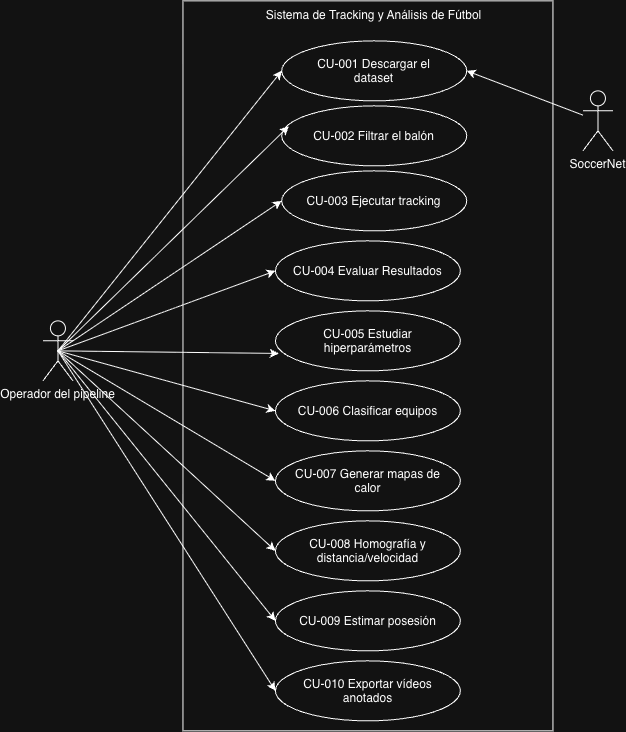
\includegraphics[width=0.9\textwidth]{figures/casosdeuso1.drawio.png}
\caption{Casos de uso del pipeline offline: el operador del pipeline y
SoccerNet como sistema externo.}
\label{fig:cu-pipeline}
\end{figure}

\begin{figure}[htp]
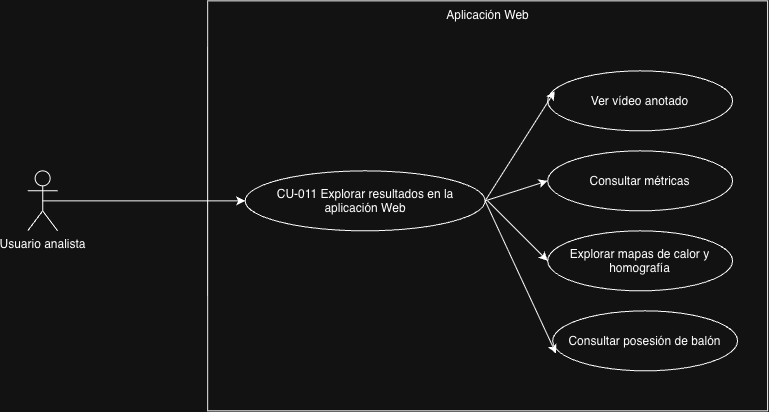
\includegraphics[width=0.9\textwidth]{figures/casosdeuso2.drawio.png}
\caption{Caso de uso de la aplicación web: el usuario analista
explora los resultados a través de cuatro comportamientos incluidos.}
\label{fig:cu-web}
\end{figure}

\begin{table}[htp]
\centering
\caption{CU-001: Descargar el dataset.}
\label{tab:cu-001}
\renewcommand{\arraystretch}{1.2}
\begin{tabular}{|p{3.1cm}|p{9.2cm}|}
\hline
\rowcolor{gray!25}
\multicolumn{2}{|l|}{\textbf{CU-001 -- Descargar el dataset}} \\
\hline
Actor & Operador del pipeline \\
\hline
Descripción & El operador ejecuta la descarga de las secuencias de
  SoccerNet-Tracking mediante la API oficial. \\
\hline
Precondiciones & Acceso a la API de SoccerNet. \\
\hline
Flujo principal & 1) El operador ejecuta
  \texttt{soccernet\_download.py}. 2) El sistema descarga las secuencias de
  train, test y \emph{challenge}. 3) Las almacena en la estructura de
  carpetas esperada por el resto del pipeline. \\
\hline
Postcondiciones & Dataset disponible localmente para el resto de casos de
  uso. \\
\hline
\end{tabular}
\end{table}

\begin{table}[htp]
\centering
\caption{CU-002: Filtrar el balón de las detecciones.}
\label{tab:cu-002}
\renewcommand{\arraystretch}{1.2}
\begin{tabular}{|p{3.1cm}|p{9.2cm}|}
\hline
\rowcolor{gray!25}
\multicolumn{2}{|l|}{\textbf{CU-002 -- Filtrar el balón de las detecciones}} \\
\hline
Actor & Operador del pipeline \\
\hline
Descripción & El sistema separa las detecciones de balón del resto antes de
  pasarlas al tracker. \\
\hline
Precondiciones & \texttt{det.txt} de la secuencia disponible. \\
\hline
Flujo principal & 1) El sistema lee cada detección del frame. 2) Calcula su
  área y su ratio ancho y alto. 3) La clasifica como balón o jugador según
  los umbrales del filtro geométrico. \\
\hline
Postcondiciones & Detecciones de jugadores separadas de las de balón, listas
  para el tracking. \\
\hline
\end{tabular}
\end{table}

\begin{table}[htp]
\centering
\caption{CU-003: Ejecutar tracking (ByteTrack / OC-SORT).}
\label{tab:cu-003}
\renewcommand{\arraystretch}{1.2}
\begin{tabular}{|p{3.1cm}|p{9.2cm}|}
\hline
\rowcolor{gray!25}
\multicolumn{2}{|l|}{\textbf{CU-003 -- Ejecutar tracking}} \\
\hline
Actor & Operador del pipeline \\
\hline
Descripción & El operador ejecuta uno o ambos algoritmos de tracking sobre
  una o todas las secuencias de un split. \\
\hline
Precondiciones & Detecciones de jugadores filtradas disponibles. \\
\hline
Flujo principal & 1) El operador lanza \texttt{run\_all\_train.py} o
  \texttt{run\_all\_test.py}. 2) El sistema inicializa el tracker
  elegido. 3) Actualiza el tracker frame a frame con las detecciones. 4)
  Persiste los resultados en formato MOT (IRQ-004). \\
\hline
Postcondiciones & Resultados de tracking disponibles para su evaluación. \\
\hline
\end{tabular}
\end{table}

\begin{table}[htp]
\centering
\caption{CU-004: Evaluar resultados de tracking.}
\label{tab:cu-004}
\renewcommand{\arraystretch}{1.2}
\begin{tabular}{|p{3.1cm}|p{9.2cm}|}
\hline
\rowcolor{gray!25}
\multicolumn{2}{|l|}{\textbf{CU-004 -- Evaluar resultados de tracking}} \\
\hline
Actor & Operador del pipeline \\
\hline
Descripción & El operador evalúa los resultados de tracking con
  \texttt{TrackEval}. \\
\hline
Precondiciones & Resultados de tracking y \emph{ground truth}
  disponibles. \\
\hline
Flujo principal & 1) El sistema genera el \emph{seqmap} del split. 2)
  Ejecuta \texttt{TrackEval} sobre los resultados de cada algoritmo. 3)
  Persiste las métricas por secuencia y combinadas. \\
\hline
Postcondiciones & Métricas de evaluación disponibles para la comparativa
  (capítulo~\ref{cap:pruebas}). \\
\hline
\end{tabular}
\end{table}

\begin{table}[htp]
\centering
\caption{CU-005: Realizar estudio de hiperparámetros.}
\label{tab:cu-005}
\renewcommand{\arraystretch}{1.2}
\begin{tabular}{|p{3.1cm}|p{9.2cm}|}
\hline
\rowcolor{gray!25}
\multicolumn{2}{|l|}{\textbf{CU-005 -- Realizar estudio de hiperparámetros}} \\
\hline
Actor & Operador del pipeline \\
\hline
Descripción & El operador ejecuta el barrido de hiperparámetros de un
  algoritmo y obtiene su configuración óptima. \\
\hline
Precondiciones & Detecciones de test filtradas y evaluación
  disponibles. \\
\hline
Flujo principal & 1) El sistema recorre cada valor del rango de un
  hiperparámetro. 2) Ejecuta el tracking y la evaluación con ese
  valor. 3) Registra la métrica resultante. 4) Selecciona el valor con
  mejor HOTA y lo confirma con una ejecución independiente (RF-008). \\
\hline
Postcondiciones & Configuración óptima determinada y validada para el
  algoritmo. \\
\hline
\end{tabular}
\end{table}

\begin{table}[htp]
\centering
\caption{CU-006: Clasificar jugadores por equipo.}
\label{tab:cu-006}
\renewcommand{\arraystretch}{1.2}
\begin{tabular}{|p{3.1cm}|p{9.2cm}|}
\hline
\rowcolor{gray!25}
\multicolumn{2}{|l|}{\textbf{CU-006 -- Clasificar jugadores por equipo}} \\
\hline
Actor & Operador del pipeline \\
\hline
Descripción & El operador ejecuta la clasificación de equipos por color de
  camiseta sobre una secuencia. \\
\hline
Precondiciones & Resultados de tracking con la configuración óptima
 disponibles. \\
\hline
Flujo principal & 1) El sistema recorta la zona de camiseta de cada
  detección de jugador. 2) Extrae su color dominante con K-means ($k=1$).
  3) Agrupa todos los colores en dos equipos con K-means ($k=2$). 4)
  Determina el equipo mayoritario de cada \texttt{track\_id}. \\
\hline
Postcondiciones & Asignación de equipo por jugador persistida. \\
\hline
\end{tabular}
\end{table}

\begin{table}[htp]
\centering
\caption{CU-007: Generar mapas de calor.}
\label{tab:cu-007}
\renewcommand{\arraystretch}{1.2}
\begin{tabular}{|p{3.1cm}|p{9.2cm}|}
\hline
\rowcolor{gray!25}
\multicolumn{2}{|l|}{\textbf{CU-007 -- Generar mapas de calor}} \\
\hline
Actor & Operador del pipeline \\
\hline
Descripción & El operador genera los mapas de calor de ocupación del
  campo, globales y por equipo. \\
\hline
Precondiciones & Resultados de tracking y, para el mapa por
  equipo, clasificación de equipos disponibles. \\
\hline
Flujo principal & 1) El sistema proyecta las posiciones de los jugadores
  sobre el campo dibujado a escala. 2) Calcula la densidad de posiciones
  mediante estimación KDE. 3) Genera y persiste la figura. \\
\hline
Postcondiciones & Mapas de calor disponibles. \\
\hline
\end{tabular}
\end{table}

\begin{table}[htp]
\centering
\caption{CU-008: Calcular homografía y estimar distancia/velocidad.}
\label{tab:cu-008}
\renewcommand{\arraystretch}{1.2}
\begin{tabular}{|p{3.1cm}|p{9.2cm}|}
\hline
\rowcolor{gray!25}
\multicolumn{2}{|l|}{\textbf{CU-008 -- Calcular homografía y estimar distancia/velocidad}} \\
\hline
Actor & Operador del pipeline \\
\hline
Descripción & El operador calcula una homografía real sobre un tramo
  verificado y estima distancia y velocidad de los jugadores. \\
\hline
Precondiciones & Tramo de cámara estable identificado manualmente
; resultados de tracking disponibles. \\
\hline
Flujo principal & 1) El operador identifica 4 puntos de referencia en un
  frame representativo. 2) El sistema calcula la matriz de homografía y
  valida su error de reproyección. 3) Proyecta las posiciones de cada
  jugador a metros reales. 4) Calcula distancia total y velocidad media y
  de pico. \\
\hline
Postcondiciones & Distancia y velocidad por jugador persistidas. \\
\hline
\end{tabular}
\end{table}

\begin{table}[htp]
\centering
\caption{CU-009: Estimar posesión de balón.}
\label{tab:cu-009}
\renewcommand{\arraystretch}{1.2}
\begin{tabular}{|p{3.1cm}|p{9.2cm}|}
\hline
\rowcolor{gray!25}
\multicolumn{2}{|l|}{\textbf{CU-009 -- Estimar posesión de balón}} \\
\hline
Actor & Operador del pipeline \\
\hline
Descripción & El operador calcula el porcentaje de posesión de balón por
  equipo, por proximidad espacial. \\
\hline
Precondiciones & Clasificación de equipos y detecciones de balón
 disponibles. \\
\hline
Flujo principal & 1) El sistema calcula, para cada frame con balón
  detectado, el jugador más cercano. 2) Comprueba que la distancia no
  supera el umbral. 3) Asigna la posesión de ese frame al equipo
  de ese jugador. 4) Agrega el resultado en porcentaje por equipo. \\
\hline
Postcondiciones & Porcentaje de posesión por equipo persistido. \\
\hline
\end{tabular}
\end{table}

\begin{table}[htp]
\centering
\caption{CU-010: Exportar vídeos anotados.}
\label{tab:cu-010}
\renewcommand{\arraystretch}{1.2}
\begin{tabular}{|p{3.1cm}|p{9.2cm}|}
\hline
\rowcolor{gray!25}
\multicolumn{2}{|l|}{\textbf{CU-010 -- Exportar vídeos anotados}} \\
\hline
Actor & Operador del pipeline \\
\hline
Descripción & El operador genera un vídeo con las cajas e identificadores
  de tracking superpuestos, para su uso en la memoria y en la demo. \\
\hline
Precondiciones & Resultados de tracking disponibles. \\
\hline
Flujo principal & 1) El operador selecciona secuencia y algoritmo. 2) El
  sistema dibuja las cajas e identificadores sobre cada frame. 3) Codifica
  el vídeo resultante en formato \texttt{.mp4}. \\
\hline
Postcondiciones & Vídeo anotado disponible en \texttt{videos/}. \\
\hline
\end{tabular}
\end{table}

\begin{table}[htp]
\centering
\caption{CU-011: Explorar resultados en la aplicación web.}
\label{tab:cu-011}
\renewcommand{\arraystretch}{1.2}
\begin{tabular}{|p{3.1cm}|p{9.2cm}|}
\hline
\rowcolor{gray!25}
\multicolumn{2}{|l|}{\textbf{CU-011 -- Explorar resultados en la aplicación web}} \\
\hline
Actor & Usuario analista \\
\hline
Descripción & El usuario explora los resultados del proyecto a través de
  dos vistas: una comparativa global de métricas entre algoritmos, y un
  explorador por secuencia y algoritmo con el vídeo anotado y los
  metadatos deportivos generados, sin recálculo en el navegador. Incluye:
  ver vídeo anotado, consultar métricas comparativas, explorar mapas de
  calor y homografía, y consultar posesión de balón. \\
\hline
Precondiciones & Datos de visualización exportados disponibles. \\
\hline
Flujo principal & 1) El usuario abre la aplicación web, que muestra por
  defecto la comparativa global de métricas entre algoritmos. 2) El
  usuario cambia a la pestaña de exploración por secuencias y selecciona
  secuencia y algoritmo. 3) La interfaz muestra el vídeo anotado y los
  paneles de equipos y posesión. 4) El usuario consulta, opcionalmente,
  los mapas de calor y la homografía de esa secuencia. \\
\hline
Postcondiciones & El usuario obtiene una interpretación visual de los
  resultados del proyecto, agregados o por secuencia concreta. \\
\hline
\end{tabular}
\end{table}

\section{Matriz de trazabilidad}
\label{sec:analisis-trazabilidad}

La matriz de trazabilidad relaciona los requisitos de este capítulo con los
objetivos específicos OE-01 a OE-11 definidos en la
sección~\ref{sec:intro-objetivos} del capítulo~\ref{cap:introduccion}.
Sirve para comprobar que cada objetivo queda cubierto por al menos un
requisito y que ningún requisito queda desligado de los fines del proyecto.
La trazabilidad se reparte en tres tablas, correspondientes a los
requisitos de información (Tabla~\ref{tab:traza-irq}), los requisitos
funcionales (Tabla~\ref{tab:traza-rf}) y los requisitos no funcionales
junto con las reglas de negocio (Tabla~\ref{tab:traza-rnf-rn}).

\begin{table}[htp]
\centering
\footnotesize
\caption{Trazabilidad de los requisitos de información.}
\label{tab:traza-irq}
\renewcommand{\arraystretch}{1.15}
\begin{tabular}{|p{1.3cm}|*{11}{>{\centering\arraybackslash}p{0.75cm}|}}
\hline
\rowcolor{gray!25}
\textbf{Req.} & \textbf{OE-01} & \textbf{OE-02} & \textbf{OE-03} & \textbf{OE-04} & \textbf{OE-05} & \textbf{OE-06} & \textbf{OE-07} & \textbf{OE-08} & \textbf{OE-09} & \textbf{OE-10} & \textbf{OE-11} \\
\hline
IRQ-001 & X & & & & & & & & & & \\
\hline
IRQ-002 & X & & & X & & & & & & & \\
\hline
IRQ-003 & X & & & & & & & & & & \\
\hline
IRQ-004 & & X & X & X & X & & & & & & \\
\hline
IRQ-005 & & & & X & X & & & & & & \\
\hline
IRQ-006 & & & & & X & & & & & & \\
\hline
IRQ-007 & & & & & & X & X & & X & & \\
\hline
IRQ-008 & & & & & & & X & X & X & & \\
\hline
IRQ-009 & & & & & & & & & & & X \\
\hline
\end{tabular}
\end{table}

\begin{table}[htp]
\centering
\footnotesize
\caption{Trazabilidad de los requisitos funcionales.}
\label{tab:traza-rf}
\renewcommand{\arraystretch}{1.15}
\begin{tabular}{|p{1.3cm}|*{11}{>{\centering\arraybackslash}p{0.75cm}|}}
\hline
\rowcolor{gray!25}
\textbf{Req.} & \textbf{OE-01} & \textbf{OE-02} & \textbf{OE-03} & \textbf{OE-04} & \textbf{OE-05} & \textbf{OE-06} & \textbf{OE-07} & \textbf{OE-08} & \textbf{OE-09} & \textbf{OE-10} & \textbf{OE-11} \\
\hline
RF-001 & X & & & & & & & & & & \\
\hline
RF-002 & & X & & & & & & & & & \\
\hline
RF-003 & & X & & & & & & & & & \\
\hline
RF-004 & & X & & & & & & & & & \\
\hline
RF-005 & & & X & & & & & & & & \\
\hline
RF-006 & & & & X & & & & & & & \\
\hline
RF-007 & & & & & X & & & & & & \\
\hline
RF-008 & & & & & X & & & & & & \\
\hline
RF-009 & & & & & X & & & & & & \\
\hline
RF-010 & & & & & & X & & & & & \\
\hline
RF-011 & & & & & & X & & & & & \\
\hline
RF-012 & & & & & & & X & & & & \\
\hline
RF-013 & & & & & & & & X & & & \\
\hline
RF-014 & & & & & & & & X & & & \\
\hline
RF-015 & & & & & & & & & X & & \\
\hline
RF-016 & & & & & & & & & & X & \\
\hline
RF-017 & & & & & & & & & & & X \\
\hline
\end{tabular}
\end{table}

\clearpage

\begin{table}[htp]
\centering
\footnotesize
\caption{Trazabilidad de requisitos no funcionales y reglas de negocio.}
\label{tab:traza-rnf-rn}
\renewcommand{\arraystretch}{1.15}
\begin{tabular}{|p{1.3cm}|*{11}{>{\centering\arraybackslash}p{0.75cm}|}}
\hline
\rowcolor{gray!25}
\textbf{Req.} & \textbf{OE-01} & \textbf{OE-02} & \textbf{OE-03} & \textbf{OE-04} & \textbf{OE-05} & \textbf{OE-06} & \textbf{OE-07} & \textbf{OE-08} & \textbf{OE-09} & \textbf{OE-10} & \textbf{OE-11} \\
\hline
RNF-001 & & & & & & & & & & X & \\
\hline
RNF-002 & & & X & & & & & & & & \\
\hline
RNF-003 & & & & & & & & & & X & \\
\hline
RNF-004 & & X & & & & & & & & & \\
\hline
RNF-005 & & & & & & & & & & X & \\
\hline
RNF-006 & & & & & & & & & & X & \\
\hline
RNF-007 & & & & & & & & & & & X \\
\hline
RNF-008 & & & & & & & & & & & X \\
\hline
RNF-009 & & & & & & & & & & & X \\
\hline
RN-001 & & X & & & & & & & & & \\
\hline
RN-002 & & & & X & & & & & & & \\
\hline
RN-003 & & & & & X & & & & & & \\
\hline
RN-004 & & & & & & X & & & & & \\
\hline
RN-005 & & & & & & & & X & & & \\
\hline
RN-006 & & & & & & & & & X & & \\
\hline
\end{tabular}
\end{table}

La lectura de las tres tablas muestra que los once objetivos específicos
reciben al menos una traza y que ningún requisito queda aislado. El
objetivo OE-10 (documentar las limitaciones técnicas)
recibe trazas exclusivamente de requisitos no funcionales, coherente con su
naturaleza transversal: no se satisface con una funcionalidad concreta,
sino con un criterio de calidad aplicado a todas las demás
(sección~\ref{sec:gestion-calidad}).

    \chapter{Diseño}
\label{cap:diseno}

Este capítulo presenta el diseño del sistema desarrollado en este proyecto. Este capítulo se centra en el
\emph{qué} y el \emph{por qué} de cada diseño, no en el \emph{cómo} se ha implementado, que se detalla en el capítulo~\ref{cap:implementacion}.

\section{Arquitectura general}
\label{sec:diseno-arquitectura}

Como se avanzó en el capítulo~\ref{cap:analisis}
(Figura~\ref{fig:analisis-contexto}), el sistema se organiza en dos bloques
muy distintos: un \textbf{pipeline offline} en Python, y una \textbf{aplicación web} de visualización
que consume los resultados ya calculados. La
Figura~\ref{fig:diseno-arquitectura} representa esta arquitectura a nivel de
componentes: no las funcionalidades concretas de cada fase --eso se detalla
en las secciones siguientes de este capítulo--, sino los grandes bloques del
sistema y cómo se comunican entre sí.

\begin{figure}[htp]
\centering
\begin{tikzpicture}[
  every node/.style={align=center, font=\footnotesize},
  box/.style={draw, rounded corners, fill=blue!8, minimum width=3.4cm, minimum height=1.1cm},
  arrow/.style={-{Latex[length=2.5mm]}, thick}
]
\node[box, fill=gray!12] (dataset) {SoccerNet-Tracking\\(dataset externo)};
\node[box, right=1.6cm of dataset] (pipeline) {Pipeline offline\\(Python)};
\node[box, below=1.3cm of pipeline, minimum width=5.2cm, fill=yellow!12] (storage) {Artefactos persistidos en disco\\\footnotesize\texttt{.txt / .csv / .png / .mp4 / .json}};
\node[box, right=1.6cm of pipeline, fill=orange!10] (web) {Aplicación web\\(React + Vite + TS)};
\draw[arrow] (dataset) -- (pipeline) node[midway, above, font=\tiny] {\texttt{det.txt}, \texttt{gt.txt}};
\draw[arrow] (pipeline) -- (storage);
\draw[arrow] (storage) -- (web) node[midway, above, font=\tiny, sloped] {paquete exportado};
\draw[arrow] (storage.north) to[out=100, in=260] node[midway, left, font=\tiny] {reanuda desde cualquier fase} (pipeline.south);
\end{tikzpicture}
\caption{Arquitectura general del sistema, a nivel de componentes: el
pipeline offline persiste todo su trabajo en disco en vez de mantener
estado en memoria, y la aplicación web consume ese mismo almacenamiento ya
calculado, sin recalcular nada ni compartir proceso con el pipeline.}
\label{fig:diseno-arquitectura}
\end{figure}

Esta arquitectura por artefactos persistidos tiene tres ventajas de diseño
aprovechadas en este proyecto. Primero, permite
\textbf{reanudar} el trabajo desde cualquier fase sin repetir las
anteriores: el estudio de hiperparámetros (sección~\ref{sec:diseno-hiperparametros})
se apoya en resultados de tracking ya calculados, y el pipeline de
metadatos (sección~\ref{sec:diseno-metadatos}) se apoya en la configuración
óptima ya validada, sin necesidad de volver a ejecutar el tracking desde
cero cada vez. Segundo, favorece la \textbf{reproducibilidad}
(RNF-001): cualquier resultado puede auditarse inspeccionando el artefacto
correspondiente. Tercero,
es la base que permite a la aplicación web
(sección~\ref{sec:diseno-web}) limitarse a consumir artefactos estáticos.

\section{Diseño del pipeline de tracking}
\label{sec:diseno-tracking}

El pipeline de tracking transforma las detecciones precomputadas de una
secuencia en trayectorias con identidad consistente,
aplicando el algoritmo de tracking correspondiente
(sección~\ref{sec:fundamentos-algoritmos}). Se compone de tres bloques de
diseño: el filtrado del balón, la ejecución del algoritmo de tracking sobre
una única secuencia, y la orquestación de esa ejecución sobre la totalidad
de un split.

\subsection{Diseño del filtrado del balón}
\label{subsec:diseno-balon}

Como se justificó en la sección~\ref{subsec:fundamentos-balon}, el balón se
separa de las detecciones de personas mediante un filtro geométrico, no
mediante un detector entrenado. El diseño de este filtro es deliberadamente
simple: para cada detección del frame, se evalúan dos condiciones
independientes sobre su caja delimitadora: su área en píxeles y su
proporción ancho/alto, y solo si ambas se cumplen a la vez la detección
se aparta del flujo de tracking de personas, como ilustra la
Figura~\ref{fig:diseno-balon}. Los valores concretos de los dos umbrales
empleados se detallan y justifican en la
sección~\ref{sec:implementacion-tracking}.

\begin{figure}[htp]
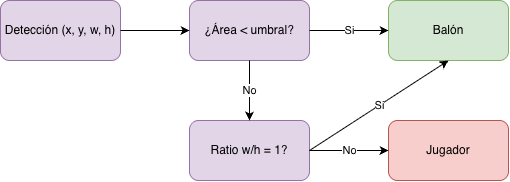
\includegraphics[width=0.85\textwidth]{figures/disenobalon.drawio.png}
\caption{Diseño del filtro geométrico de separación del balón: dos
condiciones sobre área y proporción de la caja delimitadora, evaluadas
sobre cada detección de cada frame antes de invocar al tracker.}
\label{fig:diseno-balon}
\end{figure}

\subsection{Diseño de los algoritmos de tracking}
\label{subsec:diseno-tracking-algoritmos}

Los dos algoritmos comparados (ByteTrack y OC-SORT)
se ejecutan a través de la interfaz común que expone la librería
\texttt{boxmot} (sección~\ref{sec:analisis-decision}), lo que permite que el
diseño del bucle principal de procesamiento sea idéntico para ambos y solo
cambie la clase de tracker instanciada. Este diseño responde directamente al
requisito de extensibilidad (RNF-004): incorporar un tercer algoritmo
disponible en \texttt{boxmot} no exige rediseñar el bucle, solo
instanciarlo. La Figura~\ref{fig:diseno-tracking-loop} representa este
bucle, común a ambos algoritmos.

\begin{figure}[htp]
\centering
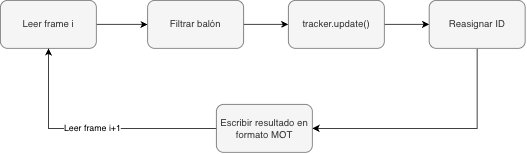
\includegraphics[width=0.85\textwidth]{figures/diseno_trackers.drawio.png}
\caption{Bucle de procesamiento común a ambos algoritmos de tracking.}
\label{fig:diseno-tracking-loop}
\end{figure}

El paso de \textbf{reasignación de identificador} merece un diseño propio:
los algoritmos de \texttt{boxmot} generan identificadores internos
arbitrarios y no necesariamente consecutivos, mientras que el formato MOT
esperado por \texttt{TrackEval} y por la interpretación humana de los
resultados es más claro con una numeración secuencial 1..N por secuencia.
El diseño mantiene, por tanto, una tabla de correspondencia
\emph{identificador interno del tracker} $\to$ \emph{identificador
secuencial}, poblada de forma que cada vez que se encuentra un nuevo
identificador interno, se le asigna el siguiente número secuencial
disponible.

\subsection{Diseño de la ejecución batch sobre un split completo}
\label{subsec:diseno-batch}

Ejecutar manualmente cada algoritmo sobre cada una de las secuencias de un
split sería inviable en la práctica y,
sobre todo, propenso a inconsistencias entre secuencias (parámetros
distintos por descuido, secuencias olvidadas). El diseño de la ejecución
batch resuelve esto con un orquestador que recorre automáticamente todas
las secuencias de un directorio de split, aplicando a cada una el mismo
bucle de la Figura~\ref{fig:diseno-tracking-loop} para cada uno de los
algoritmos configurados, como se representa en la
Figura~\ref{fig:diseno-batch}.

\begin{figure}[htp]
\centering
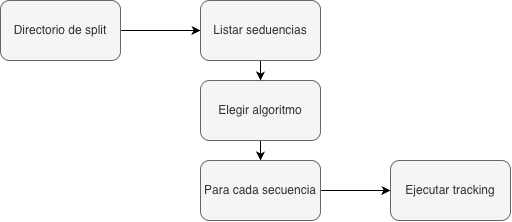
\includegraphics[width=0.85\textwidth]{figures/diseno_batch.drawio.png}
\caption{Diseño de la ejecución batch: doble bucle sobre algoritmos y
secuencias de un split, reutilizando el bucle de procesamiento de la
Figura~\ref{fig:diseno-tracking-loop} para cada combinación.}
\label{fig:diseno-batch}
\end{figure}

\section{Diseño de la evaluación}
\label{sec:diseno-evaluacion}

La evaluación traduce los resultados de tracking y el
\emph{ground truth} en las métricas de la
sección~\ref{sec:fundamentos-metricas}, delegando el cálculo en
\texttt{TrackEval} en lugar de reimplementar las métricas. El diseño de
esta fase se limita, por tanto, a preparar correctamente la entrada que
\texttt{TrackEval} espera y a configurar qué métricas calcular, como
resume la Figura~\ref{fig:diseno-evaluacion}.

\begin{figure}[htp]
\centering
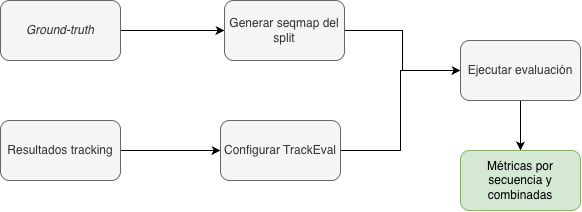
\includegraphics[width=0.85\textwidth]{figures/diseno_eval.drawio.png}
\caption{Diseño de la fase de evaluación.}
\label{fig:diseno-evaluacion}
\end{figure}

Un aspecto de diseño relevante, es que esta misma fase de
evaluación se ejecuta \textbf{dos veces con distinto propósito}: una
primera vez sobre el conjunto de entrenamiento, durante el desarrollo
inicial, y una segunda vez sobre el conjunto de test, cuyos resultados son los que finalmente se usan para las
conclusiones comparativas. El diseño
mantiene ambas ejecuciones completamente separadas.

\section{Diseño del estudio de hiperparámetros}
\label{sec:diseno-hiperparametros}

El estudio de hiperparámetros reutiliza el bucle de tracking
(Figura~\ref{fig:diseno-tracking-loop}) y la fase de evaluación
(Figura~\ref{fig:diseno-evaluacion}) como bloques ya diseñados, y añade
sobre ellos un bucle de búsqueda \emph{uno a uno}. La Figura~\ref{fig:diseno-hiperparametros} representa
este diseño.

\begin{figure}[htp]
\centering
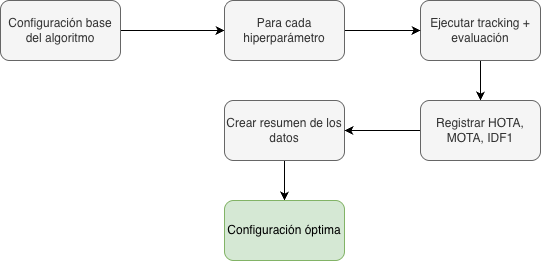
\includegraphics[width=0.85\textwidth]{figures/diseno_hiper.drawio.png}
\caption{Diseño del estudio de hiperparámetros: barrido uno a uno sobre el
conjunto de test, resumen comparativo y validación final de la
configuración óptima de cada algoritmo.}
\label{fig:diseno-hiperparametros}
\end{figure}

Este diseño es una decisión deliberada: una
búsqueda combinada crece exponencialmente con el número de parámetros y de
secuencias de test evaluadas en cada combinación, mientras que el barrido
uno a uno, con un coste lineal, permite \textbf{atribuir con
claridad} el efecto observado a un parámetro concreto, algo que
una rejilla combinada por ejemplo dificultaría al mezclar los efectos de varios
parámetros a la vez.

\section{Diseño del pipeline de metadatos}
\label{sec:diseno-metadatos}

El pipeline de metadatos parte de los resultados de tracking generados con
la configuración óptima de ByteTrack (determinada en la fase anterior) y
produce los cuatro tipos de metadatos deportivos de este proyecto. Como muestra la
Figura~\ref{fig:diseno-metadatos-dependencias}, estos cuatro bloques no son
independientes entre sí.

\begin{figure}[htp]
\centering
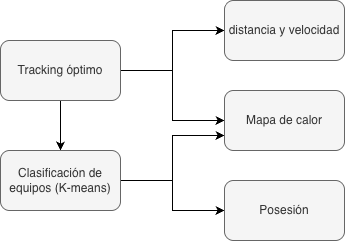
\includegraphics[width=0.85\textwidth]{figures/diseno_metadatos.drawio.png}
\caption{Dependencias entre los bloques del pipeline de metadatos.}
\label{fig:diseno-metadatos-dependencias}
\end{figure}

\subsection{Diseño de la clasificación de equipos}
\label{subsec:diseno-equipos}

La clasificación de equipos se diseña en dos niveles de K-means encadenados
(sección~\ref{sec:fundamentos-kmeans}), representados en la
Figura~\ref{fig:diseno-equipos}: primero, un K-means con $k=1$ extrae el
color dominante de la camiseta de \emph{cada} detección de jugador,
recortando la región central-superior de su caja delimitadora para evitar
incluir piernas, césped o balón en el recorte; después, un segundo K-means
con $k=2$ agrupa \emph{todos} los colores dominantes obtenidos, asumiendo
dos equipos con colores de camiseta distintos (RN-004). Por eficiencia, el
primer nivel no se aplica a todas las detecciones de la secuencia, sino a
un muestreo de frames, suficiente para determinar el equipo mayoritario de
cada \texttt{track\_id} sin procesar la secuencia completa.

\begin{figure}[htp]
\centering
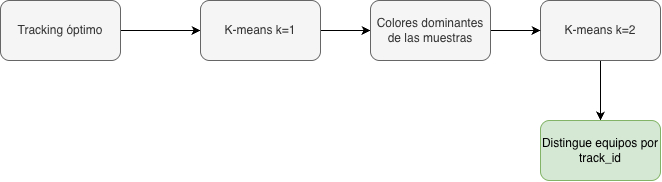
\includegraphics[width=0.85\textwidth]{figures/diseno_equipos.drawio.png}
\caption{Diseño de la clasificación de equipos: K-means en dos niveles.}
\label{fig:diseno-equipos}
\end{figure}

\begin{figure}[htp]
\centering
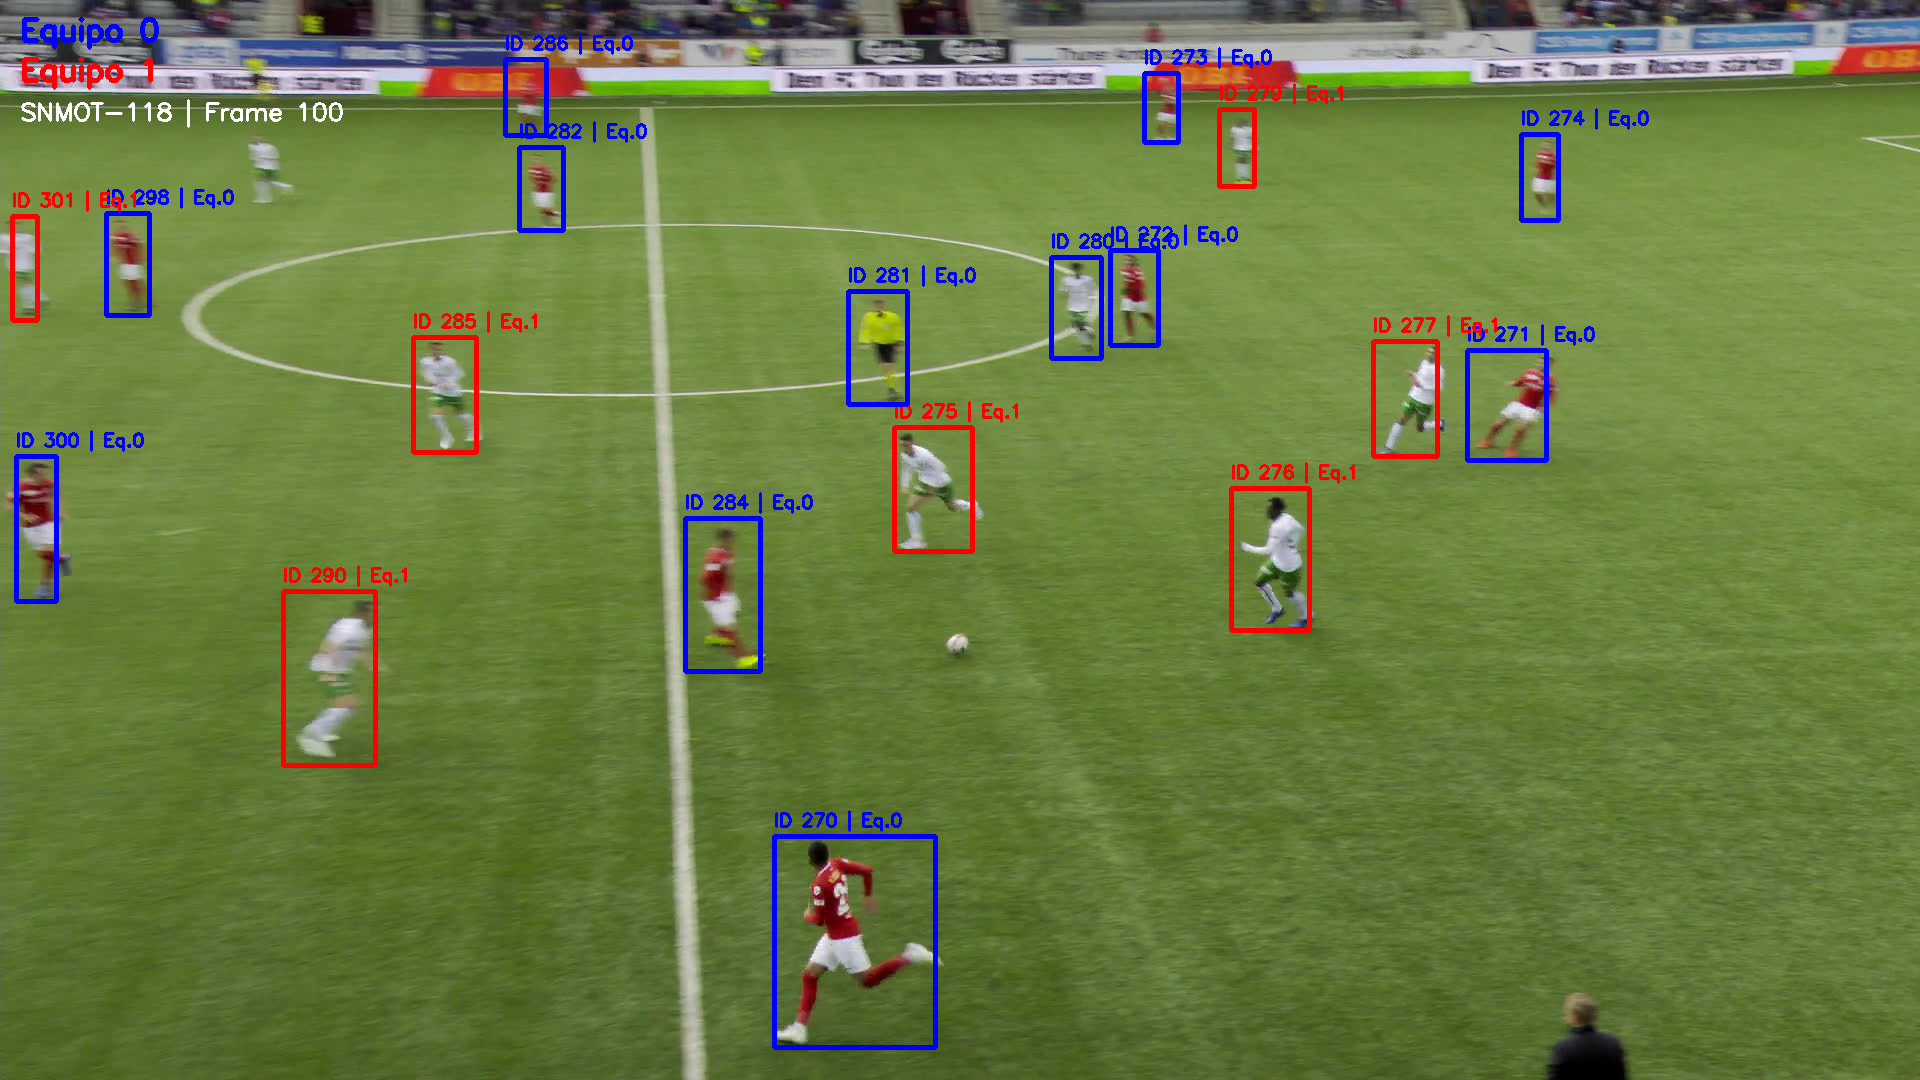
\includegraphics[width=0.85\textwidth]{figures/diseno_teams_ejemplo.png}
\caption{Resultado real de la clasificación de equipos sobre un frame de
SNMOT-118: cada jugador coloreado según el equipo asignado por K-means.}
\label{fig:diseno-teams-ejemplo}
\end{figure}

\subsection{Diseño de los mapas de calor}
\label{subsec:diseno-heatmaps}

Los mapas de calor de ocupación del campo se diseñan como una proyección de
las posiciones de tracking sobre un campo dibujado a escala
(Figura~\ref{fig:fundamentos-campo}), seguida de una estimación de densidad
por núcleos (\emph{Kernel Density Estimation}, KDE) que suaviza la nube de
puntos discretos en un mapa continuo. Se diseñan dos variantes, que
comparten el mismo procedimiento de proyección y KDE pero difieren en el
conjunto de posiciones de entrada: el mapa \textbf{general}, con todas las
posiciones de la secuencia, y el mapa \textbf{por equipo}
(sección~\ref{subsec:diseno-equipos}), que separa las posiciones según la
clasificación de equipos y usa la misma escala para ambos equipos, de modo
que sean directamente comparables entre sí.

\begin{figure}[htp]
\centering
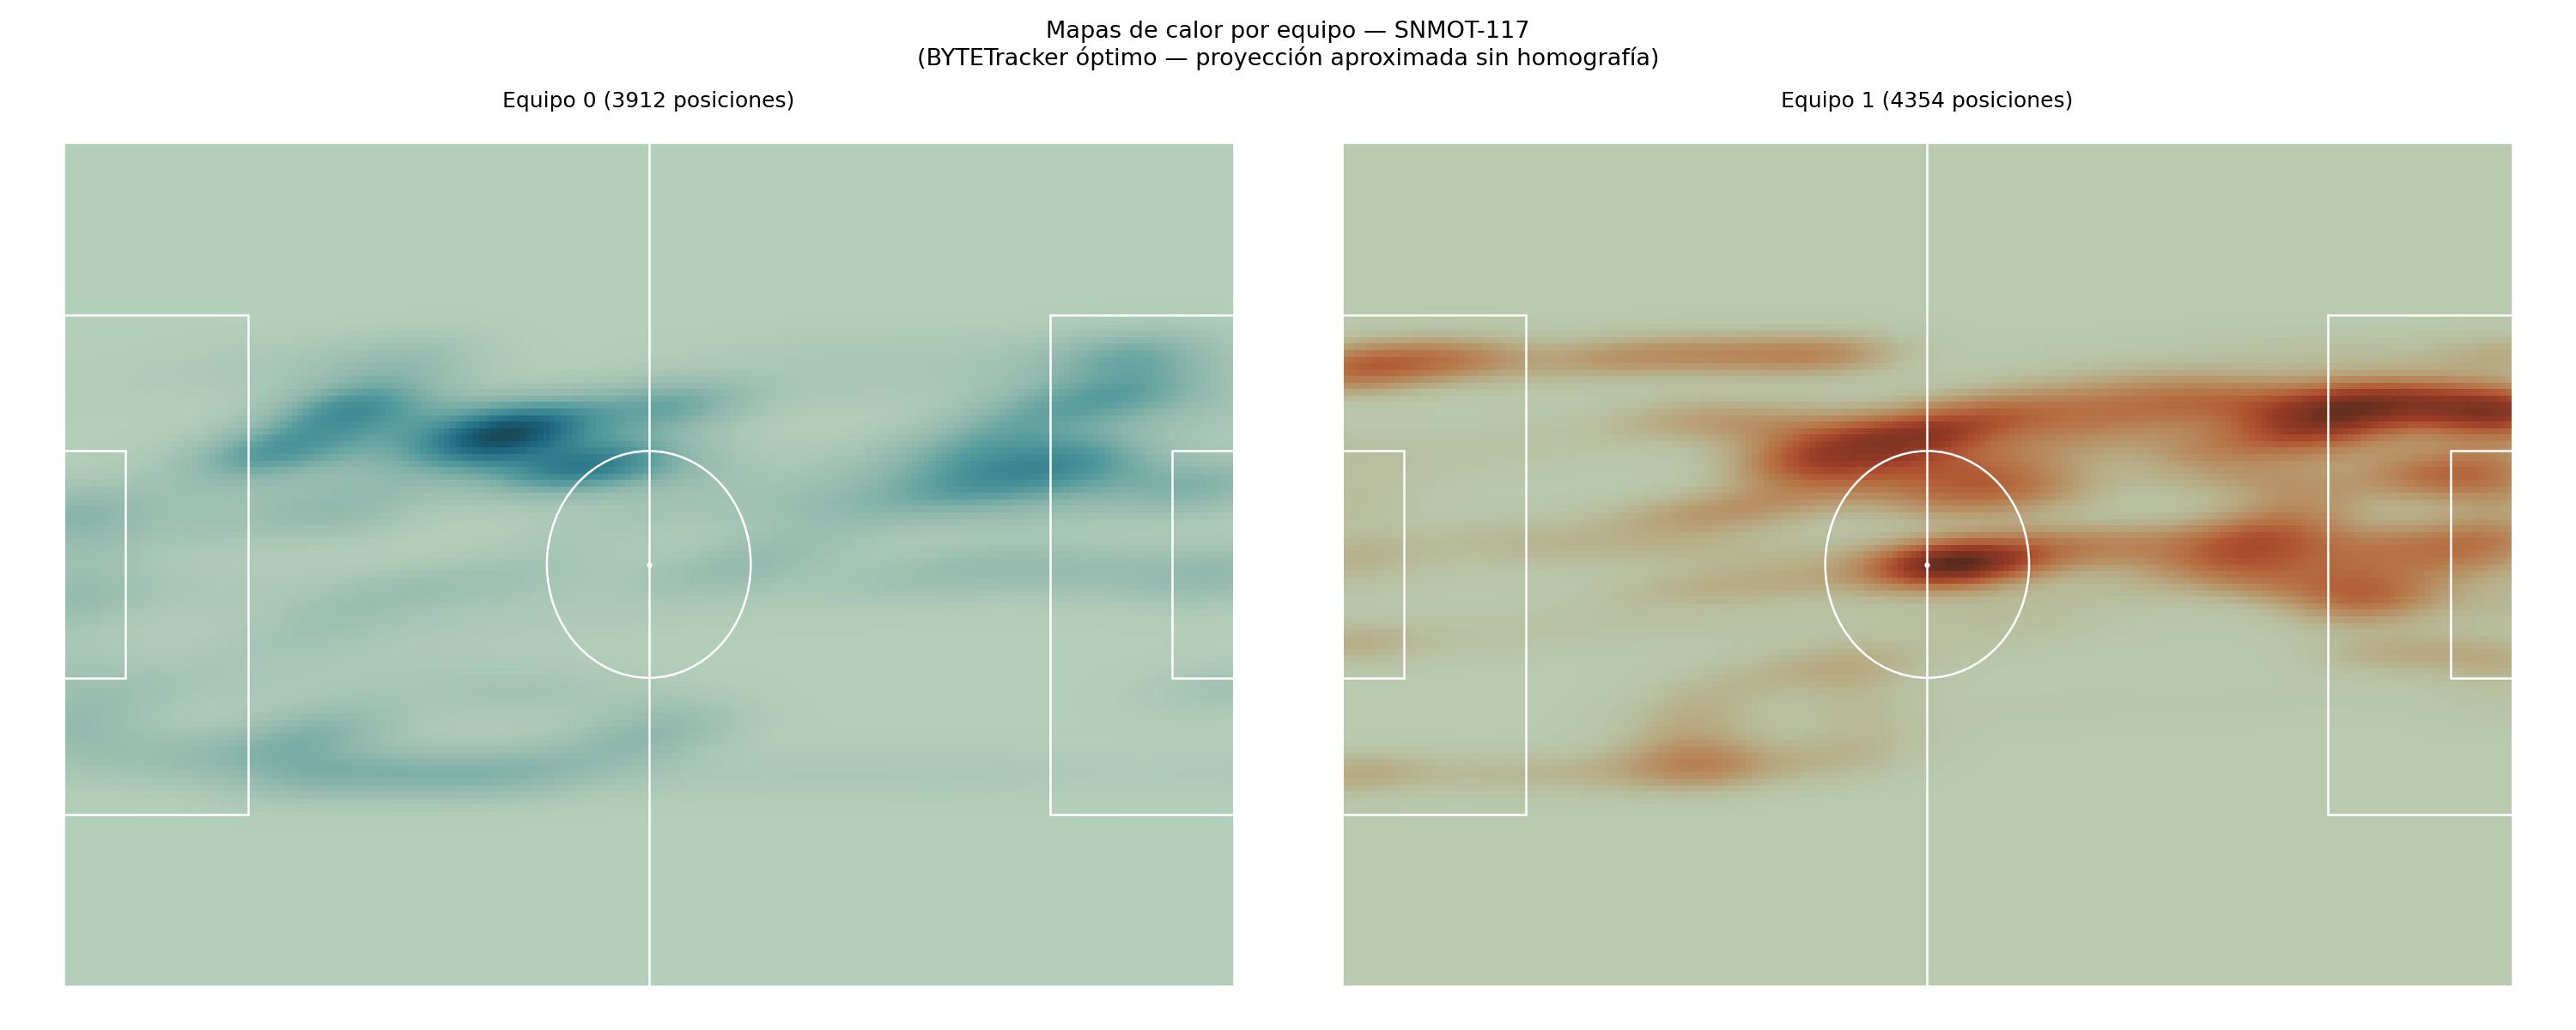
\includegraphics[width=0.95\textwidth]{figures/diseno_heatmap_by_team_ejemplo.png}
\caption{Resultado real del mapa de calor por equipo sobre SNMOT-117.}
\label{fig:diseno-heatmap-ejemplo}
\end{figure}

\subsection{Diseño de la homografía y la estimación de distancia/velocidad}
\label{subsec:diseno-homografia}

Como se explicó en la sección~\ref{sec:fundamentos-homografia}, este
proyecto distingue dos niveles de fiabilidad en la proyección de
coordenadas. El primero, usado de forma
general en los mapas de calor,
es una \textbf{proyección aproximada} que escala las posiciones observadas
por su rango directamente sobre las dimensiones del
campo. El segundo, diseñado como prueba
de concepto sobre un tramo concreto de cámara estable, es una
\textbf{homografía real}, calculada a partir de 4 puntos de referencia.
 La Figura~\ref{fig:diseno-homografia}
representa el diseño de este segundo nivel, el único que permite calcular
distancia y velocidad en unidades reales (RF-014).

\begin{figure}[htp]
\centering
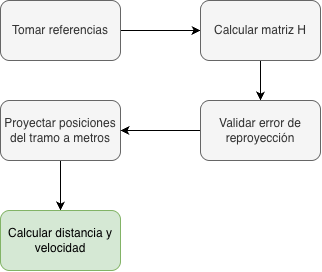
\includegraphics[width=0.85\textwidth]{figures/diseno_distancia.drawio.png}
\caption{Diseño de la homografía}
\label{fig:diseno-homografia}
\end{figure}

Un elemento de diseño importante, que se retoma como limitación en el
capítulo~\ref{cap:pruebas}, es que la zona del campo fuera del entorno
cercano a los 4 puntos de calibración no es fiable con esta homografía.
Figura~\ref{fig:diseno-heatmap-homografia-ejemplo}.

\begin{figure}[htp]
\centering
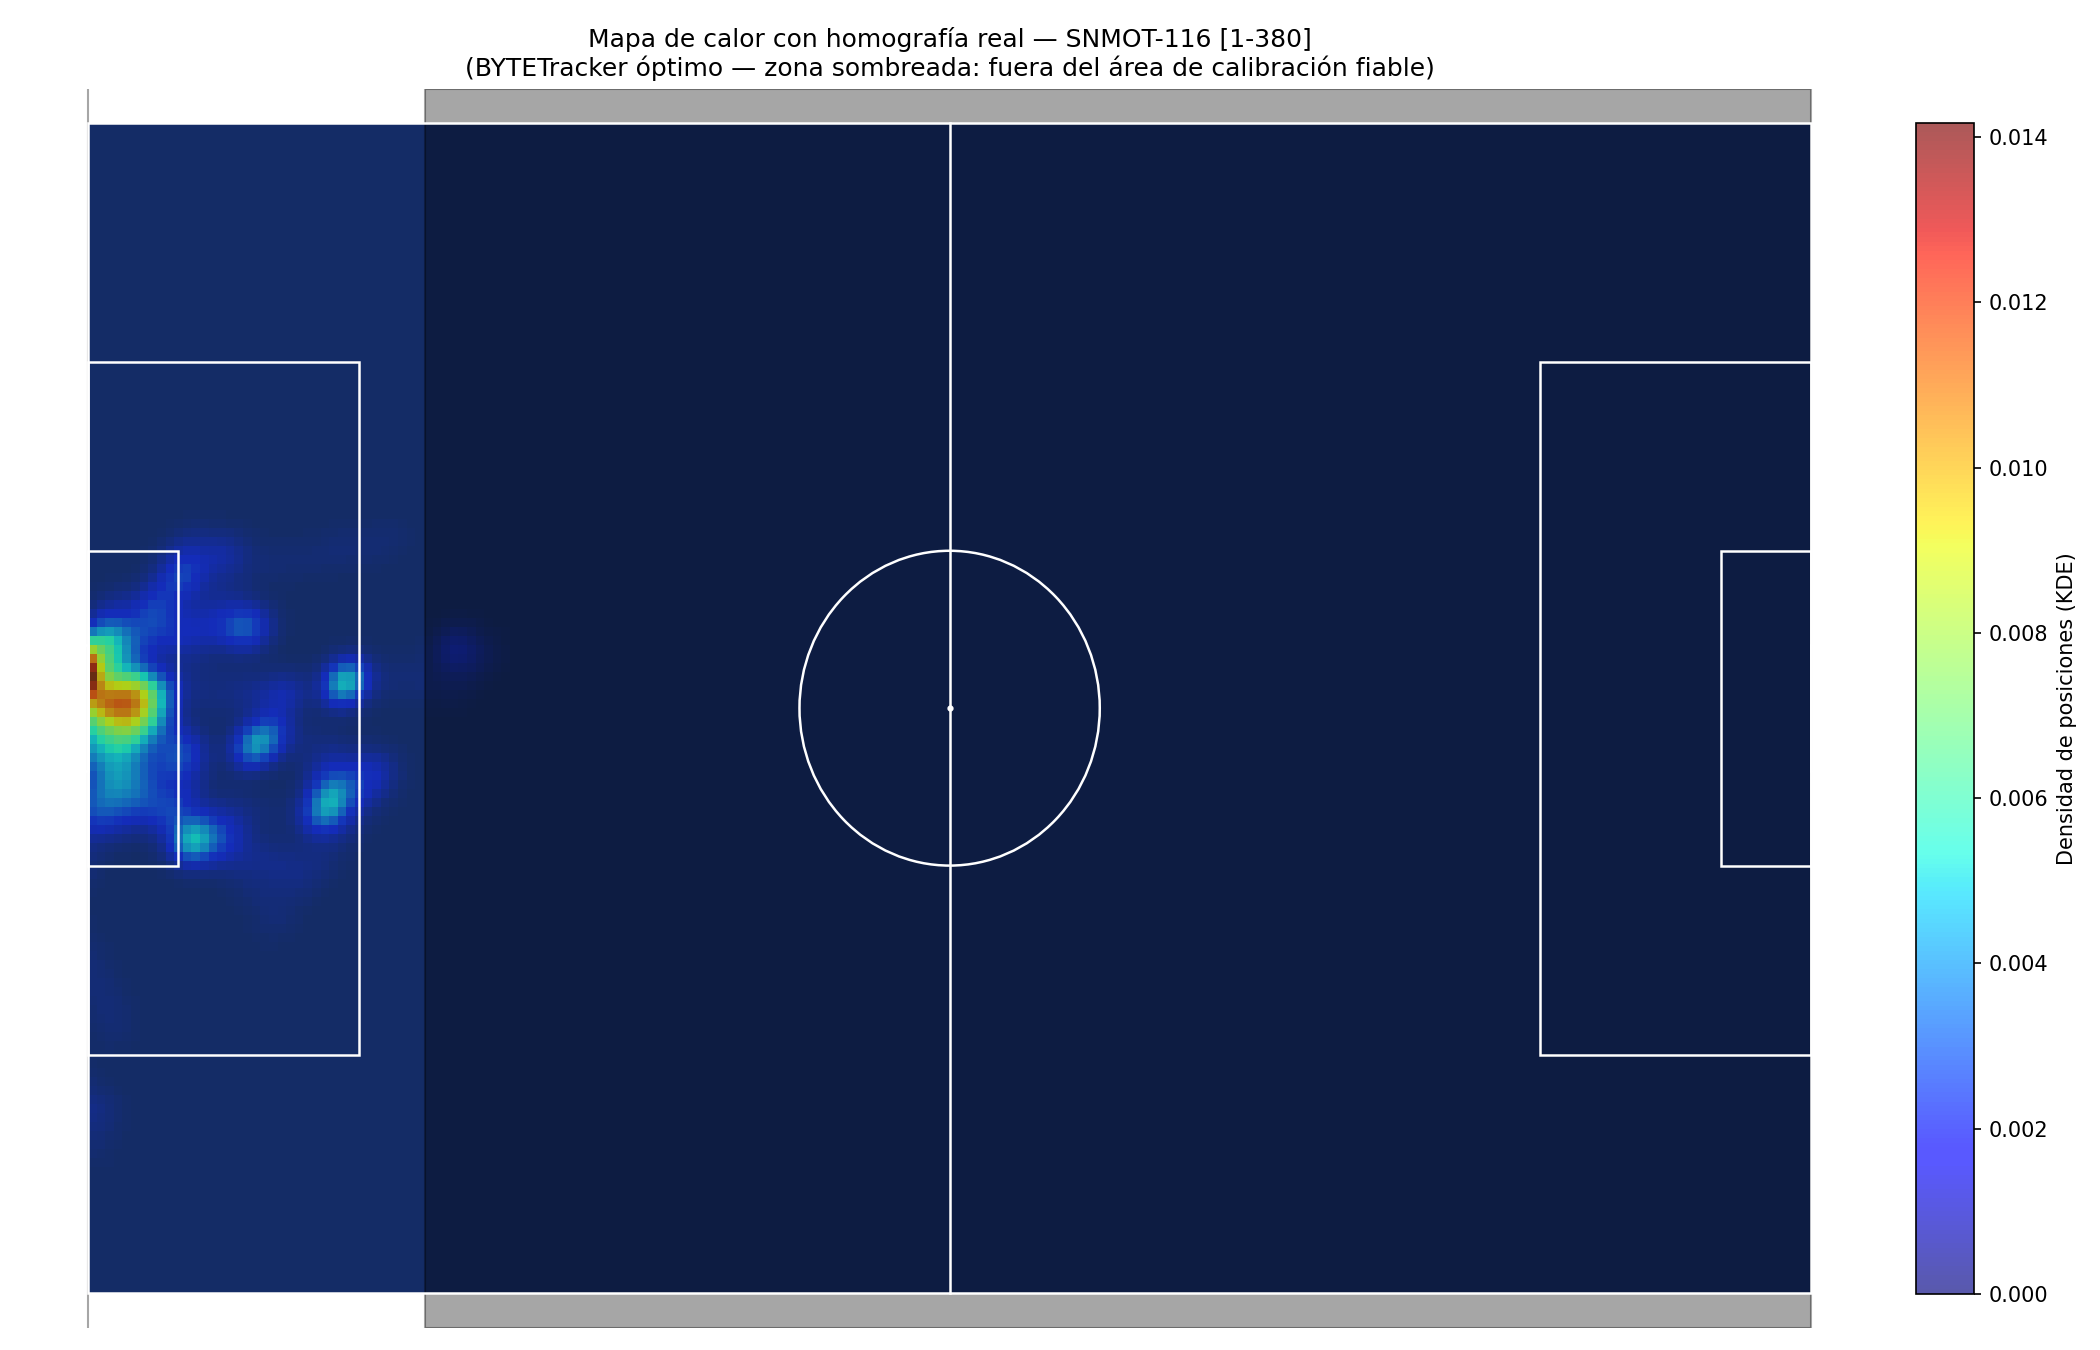
\includegraphics[width=0.85\textwidth]{figures/diseno_heatmap_homografia_ejemplo.png}
\caption{Resultado real del mapa de calor con homografía real sobre un
tramo de SNMOT-116.}
\label{fig:diseno-heatmap-homografia-ejemplo}
\end{figure}

\subsection{Diseño de la estimación de posesión}
\label{subsec:diseno-posesion}

La posesión de balón se diseña como una heurística de proximidad espacial
frame a frame. Para cada frame en que el filtro
geométrico (sección~\ref{subsec:diseno-balon}) detecta un balón, se calcula
la distancia entre su posición y la de todos los jugadores de ese frame; si
el jugador más cercano está por debajo de un umbral máximo de distancia, la posesión de ese frame se asigna a su equipo;
en caso contrario, se considera
balón suelto y el frame no cuenta para ningún equipo. La
Figura~\ref{fig:diseno-posesion} resume este diseño.

\begin{figure}[htp]
\centering
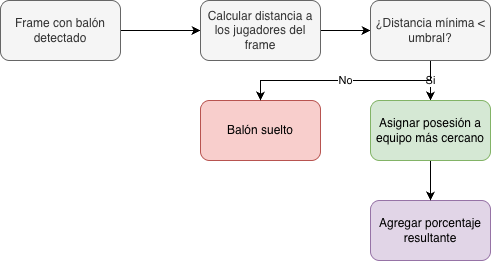
\includegraphics[width=0.85\textwidth]{figures/diseno_posesion.drawio.png}
\caption{Diseño de la estimación de posesión.}
\label{fig:diseno-posesion}
\end{figure}

\section{Diseño de datos y artefactos}
\label{sec:diseno-artefactos}

Como se ha señalado en la sección~\ref{sec:diseno-arquitectura}, el
contrato entre fases de este sistema son los artefactos que cada una
persiste en disco. La Tabla~\ref{tab:diseno-artefactos} cataloga estos
artefactos por fase, con su formato y su carpeta de salida.

\begin{table}[htp]
\centering
\caption{Catálogo de artefactos generados por cada fase del sistema.}
\label{tab:diseno-artefactos}
\renewcommand{\arraystretch}{1.2}
\small
\begin{tabular}{|p{2.9cm}|p{3.8cm}|p{1.5cm}|p{3.9cm}|}
\hline
\rowcolor{gray!25}
\textbf{Fase} & \textbf{Artefacto} & \textbf{Formato} & \textbf{Carpeta} \\
\hline
Tracking & Trayectorias por secuencia y algoritmo & \texttt{.txt} (MOT) &
  \texttt{results\_\allowbreak train/}, \texttt{results\_\allowbreak test/} \\
\hline
Evaluación & Métricas por secuencia y combinadas & \texttt{.csv},
  \texttt{.txt} & \texttt{evaluation\_\allowbreak train/}, \texttt{evaluation\_\allowbreak test/} \\
\hline
Hiperparámetros & Trayectorias y métricas por configuración & \texttt{.txt},
  \texttt{.csv} & \texttt{results\_\allowbreak hyperparam/},
  \texttt{evaluation\_\allowbreak hyperparam/} \\
\hline
Hiperparámetros & Tabla resumen y gráficas comparativas & \texttt{.csv},
  \texttt{.png} & \texttt{evaluation\_\allowbreak hyperparam/\allowbreak plots/} \\
\hline
Equipos & Muestras de color y asignación final por jugador & \texttt{.csv} &
  \texttt{metadata\_\allowbreak output/teams/} \\
\hline
Equipos & Visualización de la clasificación sobre un frame & \texttt{.png} &
  \texttt{metadata\_\allowbreak output/teams/} \\
\hline
Mapas de calor & Mapa general, por equipo y con homografía & \texttt{.png} &
  \texttt{metadata\_\allowbreak output/heatmaps/},
  \texttt{metadata\_\allowbreak output/\allowbreak heatmap\_\allowbreak homography\_\allowbreak demo/} \\
\hline
Homografía & Distancia y velocidad por jugador & \texttt{.csv} &
  \texttt{metadata\_\allowbreak output/\allowbreak distance\_\allowbreak homography\_\allowbreak demo/} \\
\hline
Posesión & Posesión por frame y resumen por equipo & \texttt{.csv} &
  \texttt{metadata\_\allowbreak output/\allowbreak possession/} \\
\hline
Exportación & Vídeos anotados & \texttt{.mp4} & \texttt{videos/} \\
\hline
\end{tabular}
\end{table}

\section{Diseño de la aplicación web}
\label{sec:diseno-web}

Esta sección presenta el diseño de la aplicación web, ya
implementada como parte de este proyecto. Se mantiene aquí, en el
capítulo de diseño, porque las decisiones arquitectónicas que se describen
a continuación se tomaron antes de programarla y se respetaron sin cambios
durante la implementación.

\subsection{Arquitectura de la aplicación web}

Siguiendo el mismo principio de artefactos persistidos de la
sección~\ref{sec:diseno-arquitectura}, la aplicación web se implementa como
una aplicación de una sola página (\emph{Single Page Application}, React +
Vite + TypeScript) que consume exclusivamente artefactos estáticos ya
exportados por el pipeline, sin ejecutar Python ni recalcular nada en el
navegador, ni base de datos, ni llamadas de red
más allá de peticiones \texttt{fetch} a ficheros JSON, PNG y MP4. 
Esta decisión, coherente con la arquitectura general del sistema, permite que
la interfaz se pueda desplegar en cualquier alojamiento estático (o
servirse en local).

Los artefactos que consume la aplicación no son los mismos ficheros
intermedios de la Tabla~\ref{tab:diseno-artefactos}, sino un paquete
derivado y empaquetado específicamente para la web por
\texttt{src/web\_export/export\_bundle.py}.

\begin{figure}[htp]
\centering
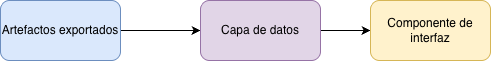
\includegraphics[width=0.85\textwidth]{figures/arquitectura_web.drawio.png}
\caption{Arquitectura de la aplicación web: los artefactos exportados por
\texttt{export\_bundle.py} alimentan una capa de datos (peticiones
\texttt{fetch} a JSON/PNG/MP4) que a su vez alimenta los componentes de
interfaz de React.}
\label{fig:diseno-web-arquitectura}
\end{figure}

\subsection{Diseño de la interfaz de usuario}
\label{subsec:diseno-web-ui}

La interfaz se organiza en dos pestañas, cada una centrada en una tarea
distinta: comparar el rendimiento agregado de los dos algoritmos, o
explorar en detalle los resultados de una secuencia concreta.

La pestaña \textbf{Comparativa de algoritmos} reproduce los resultados ya presentados en el
capítulo~\ref{cap:pruebas}: las tablas de HOTA/HOTA(0)/DetA/AssA/MOTA/IDF1
por \emph{split} (entrenamiento y test), la configuración óptima de
hiperparámetros de cada algoritmo, y las gráficas del estudio de
hiperparámetros y de la comparativa HOTA frente a HOTA(0).

La pestaña \textbf{Explorador de secuencias} (Figura~\ref{fig:diseno-web-wireframe})
está organizada en torno a una única tarea principal: seleccionar una
secuencia (SNMOT-116/117/118) evaluadas y un algoritmo (ByteTrack u OC-SORT)
mediante un selector, y explorar los resultados de esa
combinación.

No todas las combinaciones de secuencia y algoritmo tienen los mismos
datos disponibles: SNMOT-117 no tiene puntos de calibración de homografía
(sección~\ref{sec:implementacion-homografia}), y la combinación
ByteTrack/SNMOT-118 nunca llegó a generar un mapa de calor por equipo en
el pipeline original. La interfaz
muestra explícitamente una nota indicando que el dato no está disponible
para esa combinación, para que la ausencia se lea como una característica
real de los datos y no como un error de carga.

\begin{figure}[htp]
\centering
\begin{tikzpicture}[
  every node/.style={font=\footnotesize, align=center},
  panel/.style={draw, thick}
]
\draw[panel] (0,0) rectangle (12,8.6);
\draw[panel, fill=gray!8] (0,7.2) rectangle (12,8.6);
\node at (6,7.9) {\textbf{Comparativa de algoritmos} \quad|\quad \textbf{Explorador de secuencias}};
\draw[panel, fill=gray!5] (0,5.9) rectangle (12,7.2);
\node at (6,6.55) {Secuencia a elegir \quad Algoritmo a elegir};
\draw[panel, fill=blue!6] (0,3.2) rectangle (12,5.9);
\node at (6,4.55) {\textbf{Vídeo anotado}\\(cajas por equipo + ID + balón)};
\draw[panel, fill=green!6] (0,1.6) rectangle (5.9,3.2);
\node at (2.95,2.4) {\textbf{Equipos}};
\draw[panel, fill=orange!8] (6.1,1.6) rectangle (12,3.2);
\node at (9.05,2.4) {\textbf{Posesión}};
\draw[panel, fill=teal!8] (0,0) rectangle (5.9,1.6);
\node at (2.95,0.8) {\textbf{Mapas de calor}};
\draw[panel, fill=purple!8] (6.1,0) rectangle (12,1.6);
\node at (9.05,0.8) {\textbf{Homografía}};
\end{tikzpicture}
\caption{Croquis de la disposición implementada de la pestaña Explorador de secuencias}
\label{fig:diseno-web-wireframe}
\end{figure}

    \chapter{Implementación}
\label{cap:implementacion}

Este capítulo describe cómo se ha implementado, en la práctica, el diseño
presentado en el capítulo~\ref{cap:diseno}. El capítulo se cierra con una sección
dedicada explícitamente a los enfoques que se exploraron y finalmente no se
incorporaron al sistema.

\section{Entorno y herramientas}
\label{sec:implementacion-entorno}

Todo el desarrollo se ha realizado en Python 3.11, dentro de un entorno
virtual (\texttt{venv\_tfg}) situado dentro del propio repositorio, con las
dependencias fijadas en
\texttt{requirements.txt} para garantizar la reproducibilidad.
La Tabla~\ref{tab:impl-librerias} recoge las librerías con un papel directo
en el sistema. Se omiten las dependencias transitivas de bajo nivel, como
\texttt{torch} o \texttt{pandas}, que \texttt{requirements.txt} incluye por
ser un volcado completo del entorno pero que ningún
script del proyecto importa directamente: llegan al entorno como
dependencias de \texttt{boxmot} y de \texttt{ultralytics}.

\clearpage

\begin{table}[htp]
\centering
\caption{Librerías principales empleadas y su función en el sistema.}
\label{tab:impl-librerias}
\renewcommand{\arraystretch}{1.25}
\begin{tabular}{|p{2.6cm}|p{2.5cm}|p{7.0cm}|}
\hline
\rowcolor{gray!25}
\textbf{Librería} & \textbf{Versión} & \textbf{Función en el sistema} \\
\hline
\texttt{boxmot} & 10.0.43 & Implementaciones de ByteTrack y OC-SORT bajo una
  interfaz común. Versión fijada
  deliberadamente por el problema P4 de la
  Tabla~\ref{tab:impl-problemas}. \\
\hline
\texttt{trackeval} & \texttt{sn-trackeval} 0.4.0 & Evaluación con
  métricas MOT estándar
  sección. Fork de TrackEval adaptado por
  SoccerNet al formato de su benchmark. \\
\hline
\texttt{opencv-python} & 4.13.0.92 & Lectura y anotación de frames,
  cálculo de la homografía, (sección~\ref{sec:implementacion-homografia}). \\
\hline
\texttt{filterpy} & 1.4.5 & Implementación del filtro de Kalman
  (sección~\ref{subsec:fundamentos-kalman}) usada internamente por los
  trackers de \texttt{boxmot}. \\
\hline
\texttt{lapx} & 0.9.4 & Resolución del problema de asignación mediante el
  algoritmo húngaro (sección~\ref{subsec:fundamentos-hungaro}), usada
  internamente por los trackers de \texttt{boxmot}. \\
\hline
\texttt{scikit-learn} & 1.8.0 & K-means para la clasificación de equipos
  (sección~\ref{sec:fundamentos-kmeans}). \\
\hline
\texttt{scipy} & 1.17.1 & Estimación de densidad por núcleos
  (\texttt{gaussian\_kde}) en los mapas de calor. \\
\hline
\texttt{matplotlib} & 3.10.9 & Generación de todas las figuras y gráficas
  del proyecto. \\
\hline
\end{tabular}
\end{table}

Cabe señalar una inconsistencia menor detectada al redactar esta memoria:
aunque \texttt{trackeval} está instalado y en uso real en el entorno de
desarrollo (a través del paquete \texttt{sn-trackeval}), no aparece listado
de forma explícita en \texttt{requirements.txt}, lo que sugiere que ese
fichero no se regeneró tras instalarlo por separado. No afecta al
funcionamiento del proyecto en el equipo de desarrollo actual, pero es una
brecha de reproducibilidad frente al requisito RNF-001 que convendría
corregir --regenerando \texttt{requirements.txt} con \texttt{sn-trackeval}
explícitamente incluido-- antes de que un tercero intente reproducir el
entorno desde cero.

\subsection{Traslados de equipo de desarrollo}

El desarrollo no se ha mantenido en un único equipo, lo que ha exigido
recrear el entorno de trabajo en dos ocasiones: el proyecto se inició en un
portátil personal, se trasladó a mitad de desarrollo a un ordenador de
sobremesa con GPU AMD Radeon RX 6900 XT (16\,GB VRAM) en Windows, y finalmente a un equipo macOS. Cada
traslado se apoyó en el mismo mecanismo: dependencias fijadas en
\texttt{requirements.txt} y código versionado en Git, lo que permitió
recrear el entorno funcional en el nuevo equipo sin más incidencias que las
propias de cada sistema operativo.

\subsection{Problemas de entorno encontrados}
\label{subsec:implementacion-problemas}

Configurar y mantener este entorno no fue inmediato. La
Tabla~\ref{tab:impl-problemas} documenta, siguiendo el
mismo criterio de transparencia del resto de esta memoria, los catorce problemas de
entorno registrados durante el desarrollo, con su solución.

\begin{table}[htp]
\centering
\caption{Problemas de entorno encontrados durante el desarrollo y su solución.}
\label{tab:impl-problemas}
\renewcommand{\arraystretch}{1.05}
\footnotesize
\begin{tabular}{|p{0.7cm}|p{5.5cm}|p{5.3cm}|}
\hline
\rowcolor{gray!25}
\textbf{ID} & \textbf{Problema} & \textbf{Solución} \\
\hline
P1 & Python 3.14 incompatible con las librerías del proyecto &
  Fijar Python 3.11 en el entorno virtual \\
\hline
P2 & Mezcla de entornos conda y venv activos a la vez, con conflictos de
  paquetes & Desactivar conda y trabajar exclusivamente con \texttt{venv} \\
\hline
P3 & \texttt{conda activate venv\_tfg} fallaba, ya que \texttt{venv\_tfg}
  no es un entorno conda & Activar el entorno con el mecanismo propio de
  \texttt{venv} (\texttt{source venv\_tfg/bin/activate}) \\
\hline
P4 & \texttt{boxmot} v18 no expone las clases de cada tracker por separado,
  necesarias para la comparativa & Fijar la versión \texttt{10.0.43} en
  \texttt{requirements.txt} \\
\hline
P5 & Error de tipo en \texttt{kalman\_filter.py} de OC-SORT por
  incompatibilidad con la versión de NumPy instalada & Fijar
  \texttt{numpy==1.26.4} en el momento de detectarlo\footnotemark \\
\hline
P6 & Detecciones de \texttt{det.txt} con 5 columnas en lugar de las 6 que
  espera \texttt{boxmot} & Añadir manualmente la columna de clase (valor
  \texttt{0}) antes de pasar las detecciones al tracker \\
\hline
P7 & La variable de entorno \texttt{\$HOME} se colaba en comandos al
  copiar y pegar instrucciones entre terminales & Revisar manualmente los
  comandos antes de ejecutarlos \\
\hline
P8 & El entorno virtual se creó fuera de la carpeta del proyecto y VS Code
  no lo detectaba automáticamente & Recrear el entorno dentro del
  repositorio \\
\hline
P9 & Los entornos virtuales de Python no son reubicables (las rutas
  absolutas quedan grabadas en sus scripts de activación) &
  Recrearlos siempre en su ubicación final, no moverlos tras crearlos \\
\hline
P10 & \texttt{requirements.txt} estaba vacío & Regenerarlo con
  \texttt{pip freeze > requirements.txt} \\
\hline
P13 & \texttt{load\_dotenv()} no recargaba el fichero \texttt{.env} tras
  modificarlo & Forzar la recarga con \texttt{load\_dotenv(override=True)} \\
\hline
P14 & Carpetas basura generadas por rutas mal resueltas
  (\texttt{path/}, \texttt{\$HOME/}, \texttt{.venv/}, \texttt{models/}) &
  Identificarlas y eliminarlas manualmente \\
\hline
P15 & Traslado del proyecto a macOS: posible incompatibilidad de entorno &
  Entorno recreado desde \texttt{requirements.txt} sin incidencias
  destacables; solo hubo que ajustar alguna ruta de Windows a macOS \\
\hline
P17 & Los vídeos exportados con el \emph{fourcc} \texttt{mp4v} de OpenCV no
  se reproducían en el navegador & Usar el \emph{fourcc} \texttt{avc1}
  (H.264), disponible porque OpenCV, con esto, el tamaño de cada vídeo se redujo en torno a un 75\,\% \\
\hline
\end{tabular}
\end{table}
\footnotetext{El \texttt{requirements.txt} final del proyecto fija
\texttt{numpy==2.4.4}, una versión posterior a la que resolvió este
problema en su momento. Esto sugiere que la incompatibilidad original fue
resuelta más adelante en versiones posteriores de \texttt{boxmot} o de
OC-SORT, aunque no se ha vuelto a verificar explícitamente la causa
original tras la actualización.}

De estos catorce problemas, la mayoría son propios de la configuración
inicial de cualquier entorno Python (P1-P3, P8-P10) y no volvieron a
aparecer una vez resueltos. Los más relevantes para entender decisiones
posteriores de este proyecto son P4 y P6.
P17, ya en la fase de aplicación web, muestra que ese mismo tipo de
fricción de entorno no es exclusivo de Python: elegir un códec de vídeo
compatible con el navegador es un problema de la misma naturaleza en un
\emph{stack} tecnológico distinto.

\section{Estructura del repositorio}
\label{sec:implementacion-estructura}

El código del pipeline offline reside en \texttt{src/}, organizado en
paquetes por responsabilidad, resumidos en la
Tabla~\ref{tab:impl-estructura}.

\begin{table}[htp]
\centering
\caption{Paquetes del repositorio y su responsabilidad.}
\label{tab:impl-estructura}
\renewcommand{\arraystretch}{1.25}
\begin{tabular}{|p{3.6cm}|p{8.3cm}|}
\hline
\rowcolor{gray!25}
\textbf{Paquete} & \textbf{Responsabilidad} \\
\hline
\texttt{src/\allowbreak visualizacion/} & Scripts exploratorios iniciales sobre el
  \emph{ground truth}. \\
\hline
\texttt{src/\allowbreak tracking/} & Implementación de ByteTrack y OC-SORT, ejecución
  batch sobre un split completo, y exportación de vídeos anotados
  (\texttt{src/\allowbreak tracking/\allowbreak export/}). \\
\hline
\texttt{src/\allowbreak evaluation/} & Generación de \emph{seqmaps} y evaluación con
  \texttt{TrackEval} sobre train y test. \\
\hline
\texttt{src/\allowbreak hyperparameter\_\allowbreak study/} & Barrido de hiperparámetros de cada
  algoritmo, configuración óptima y resumen comparativo. \\
\hline
\texttt{src/\allowbreak metadata/} & Todo lo relacionado con la generación y gestión de metadatos. \\
\hline
\texttt{src/\allowbreak utils/} & Scripts de utilidad para tareas de un solo uso. \\
\hline
\texttt{src/\allowbreak web\_\allowbreak export/} & Generación de metadatos de OC-SORT y
  empaquetado de todos los artefactos estáticos que consume la aplicación
  web (sección~\ref{sec:implementacion-web}). \\
\hline
\end{tabular}
\end{table}

El código de la aplicación web, al no ser Python, vive fuera de
\texttt{src/}: en \texttt{frontend/}, un proyecto independiente de React.(sección~\ref{sec:implementacion-web}).

\section{Implementación del tracking}
\label{sec:implementacion-tracking}

\subsection{Scripts de visualización inicial}
\label{subsec:impl-visualizacion}

Antes de implementar ningún algoritmo de tracking, la primera fase del
proyecto se dedicó a comprender el
formato del dataset mediante scripts exploratorios, todos
ellos trabajando directamente sobre el \emph{ground truth}
(\texttt{gt.txt}) y no sobre predicciones reales de ningún tracker:
\texttt{reproducir\_vid.py} reproduce una secuencia como vídeo con OpenCV;
\texttt{bboxes\_ids.py} dibuja las cajas del \emph{ground truth} en verde
con su identificador; y \texttt{bboxes\_ids\_dif\_colors.py}
añade un color único y persistente por identificador, para facilitar el
seguimiento visual de cada jugador entre frames.

El último de estos scripts exploratorios,
\texttt{bboxes\_balltrack\_geoprop.py}, ya incorpora el filtro geométrico
de separación del balón (sección~\ref{subsec:impl-balon}) y dibuja el balón
en rojo, distinto de los jugadores. Es interesante notar que
\texttt{bboxes\_ids.py}.

\subsection{Filtrado geométrico del balón}
\label{subsec:impl-balon}

Como se diseñó en la sección~\ref{subsec:diseno-balon}, el balón se separa
de las detecciones de personas mediante dos condiciones sobre su caja
delimitadora, aplicadas de forma idéntica en todos los scripts del
proyecto que necesitan distinguir balón de jugadores:

\begin{center}
\texttt{BALL\_MAX\_AREA = 2000} \quad
\texttt{BALL\_MIN\_RATIO = 0.7} \quad
\texttt{BALL\_MAX\_RATIO = 1.3}
\end{center}

Una detección se clasifica como balón cuando su área en píxeles
($w \times h$) es inferior a \texttt{BALL\_MAX\_AREA} \emph{y}, a la vez, su
proporción $w/h$ está dentro del rango
[\texttt{BALL\_MIN\_RATIO}, \texttt{BALL\_MAX\_RATIO}], es decir, cuando la
caja es aproximadamente cuadrada. Estos tres valores se fijaron de forma
que, observando las dimensiones típicas del balón frente a las de un
jugador en las secuencias de SoccerNet, y se mantienen constantes en todo
el proyecto para que el balón se identifique de forma consistente en todas
las fases.

\subsection{ByteTrack y OC-SORT}
\label{subsec:impl-algoritmos}

Ambos algoritmos se implementan siguiendo el bucle diseñado en la
sección~\ref{subsec:diseno-tracking-algoritmos}, instanciando en cada caso la clase
correspondiente de \texttt{boxmot}: \texttt{BYTETracker()} en
\texttt{bytetracker\_alg.py}, con su configuración por defecto como punto
de partida, y
\texttt{OCSORT} también con su configuración por defecto en
\texttt{sort\_alg.py}.

El nombre \texttt{sort\_alg.py}, es una marca, documentada en la sección~\ref{subsec:fundamentos-sort}. La
intención original era implementar el SORT clásico, pero \texttt{boxmot}
en su versión fijada no expone una clase \texttt{SORT} independiente,
solo su evolución directa \texttt{OCSORT}. El fichero conserva su nombre
original como constancia de esa decisión, aunque su contenido implementa
realmente OC-SORT.

Las detecciones que llegan de \texttt{det.txt} en formato
$(x, y, w, h)$ se convierten al formato $(x_1, y_1, x_2, y_2, \text{conf},
\text{clase})$ que espera \texttt{boxmot} antes de invocar
\texttt{tracker.update()} en cada frame, y el resultado se reasigna a una numeración secuencial
mediante un diccionario de correspondencia, antes de escribirse en
el fichero de resultados con el formato MOT estándar.

\subsection{Ejecución batch y reorganización de resultados}

La ejecución sobre la totalidad de un split se implementa en
\texttt{run\_all\_train.py} y \texttt{run\_all\_test.py}, que recorren
todas las secuencias del directorio del split correspondiente y aplican,
para cada una y cada algoritmo configurado, el mismo bucle de tracking
descrito en la sección anterior (Figura~\ref{fig:diseno-batch}). Ambos
scripts comparten la misma lógica de filtrado del balón y de escritura de
resultados que las versiones de un único algoritmo y una única secuencia.

En una primera versión del proyecto, los
resultados de cada secuencia se escribían en una subcarpeta propia
(\texttt{results/bytetracker/SNMOT-060/SNMOT-060.txt}), estructura que
\texttt{TrackEval} no esperaba de forma directa. Este script recorrió una
única vez los resultados ya generados y los aplanó a la estructura que
finalmente adopta el proyecto (\texttt{results/bytetracker/SNMOT-060.txt}),
sin necesidad de rehacer el tracking desde cero. No forma parte del flujo
habitual de ejecución del sistema, pero se conserva en el repositorio como
constancia de esa reorganización.

\section{Implementación de la evaluación}
\label{sec:implementacion-evaluacion}

La evaluación se
implementa en dos scripts,
\texttt{evaluate\_train.py} y \texttt{evaluate\_test.py}, que configuran
\texttt{TrackEval} con los mismos parámetros salvo el split evaluado:

\begin{center}
\begin{minipage}{0.85\textwidth}
\begin{verbatim}
dataset_config['BENCHMARK']          = 'SoccerNet'
dataset_config['TRACKERS_TO_EVAL']   = ['bytetracker', 'ocsort']
dataset_config['SKIP_SPLIT_FOL']     = True
dataset_config['DO_PREPROC']         = False
metrics_config = {'METRICS': ['HOTA', 'MOTA', 'IDF1'], 'THRESHOLD': 0.5}
\end{verbatim}
\end{minipage}
\end{center}

donde \texttt{BENCHMARK = 'SoccerNet'} indica a \texttt{TrackEval} que use
el \emph{seqmap} generado por
\texttt{seqmaps\_creation\_test.py}/\texttt{seqmpas\_creation\_train.py}
(sección~\ref{sec:diseno-evaluacion}) en lugar de un benchmark predefinido,
y \texttt{THRESHOLD = 0.5} fija el umbral de IoU al que se calculan MOTA e
IDF1, ambas métricas de umbral único.

\subsection{Aclaración metodológica: HOTA frente a HOTA(0)}
\label{subsec:impl-hota-vs-hota0}

Antes de presentar cualquier resultado numérico en el
capítulo~\ref{cap:pruebas}, es necesario dejar constancia de un matiz
metodológico detectado al preparar esta memoria, en cumplimiento del
requisito de documentación honesta. \texttt{TrackEval} exporta,
entre sus columnas de salida, tanto \textbf{HOTA}, promediada sobre el
rango completo de umbrales de IoU de 0,05 a 0,95, como
\textbf{HOTA(0)}\footnote{La notación \texttt{HOTA(0)} es la que usa
\texttt{TrackEval} internamente para referirse al valor de HOTA en el
primer umbral de su rango de evaluación, que con la configuración de este
proyecto (\texttt{THRESHOLD = 0.5}) coincide con el umbral de 0,5 usado
también por MOTA e IDF1.}.

El script de resumen del estudio de hiperparámetros
(\texttt{summarize\_hyperparam.py}) lee explícitamente la columna
\texttt{HOTA(0)} de cada resultado:

\begin{center}
\begin{minipage}{0.8\textwidth}
\begin{verbatim}
hota = float(row.get('HOTA(0)', row.get('HOTA___50', 0))) * 100
\end{verbatim}
\end{minipage}
\end{center}

lo que significa que \textbf{todos los valores de ``HOTA'' reportados en
el estudio de hiperparámetros de este proyecto}
\textbf{son en realidad HOTA(0)}, es decir, HOTA evaluada únicamente al
50\,\% de solapamiento IoU, y no la métrica HOTA integrada que
describe la sección~\ref{subsec:fundamentos-hota}. Ambas son métricas
válidas y ambas las calcula \texttt{TrackEval} de forma estándar, pero no
son intercambiables: al integrar sobre un rango de umbrales en lugar de
uno solo, la HOTA completa es más exigente y, en general, produce un valor
distinto.
El capítulo~\ref{cap:pruebas} presenta ambos valores por separado allí
donde la distinción afecta a las conclusiones, y este matiz se retoma
explícitamente donde corresponda para no inducir a una lectura equivocada
de los resultados.

\section{Implementación del estudio de hiperparámetros}
\label{sec:implementacion-hiperparametros}

El estudio de hiperparámetros se aplica siempre sobre el
conjunto de \textbf{test}, para que la
configuración resultante no esté ajustada a datos ya vistos durante el
desarrollo inicial. Cada algoritmo tiene su propia configuración base y su
propio rango de búsqueda por hiperparámetro, recogidos en la
Tabla~\ref{tab:impl-hiperparametros-espacio}.

\begin{table}[htp]
\centering
\caption{Configuración base y rango de búsqueda de cada hiperparámetro.}
\label{tab:impl-hiperparametros-espacio}
\renewcommand{\arraystretch}{1.25}
\begin{tabular}{|p{2.6cm}|p{3.1cm}|p{1.6cm}|p{5.7cm}|}
\hline
\rowcolor{gray!25}
\textbf{Algoritmo} & \textbf{Hiperparámetro} & \textbf{Base} & \textbf{Rango de búsqueda} \\
\hline
\multirow{3}{*}{ByteTrack} & \texttt{track\_thresh} & 0.45 & 0.2, 0.3, 0.45, 0.6 \\
\cline{2-4}
 & \texttt{match\_thresh} & 0.8 & 0.6, 0.7, 0.8, 0.9 \\
\cline{2-4}
 & \texttt{track\_buffer} & 25 & 10, 20, 25, 40 \\
\hline
\multirow{4}{*}{OC-SORT} & \texttt{det\_thresh} & 0.3 & 0.1, 0.2, 0.3, 0.4, 0.5 \\
\cline{2-4}
 & \texttt{max\_age} & 30 & 10, 20, 30, 50 \\
\cline{2-4}
 & \texttt{min\_hits} & 3 & 1, 2, 3, 5 \\
\cline{2-4}
 & \texttt{iou\_threshold} & 0.3 & 0.1, 0.2, 0.3, 0.4, 0.5 \\
\hline
\end{tabular}
\end{table}

Los hiperparámetros \texttt{track\_thresh} (ByteTrack) y
\texttt{det\_thresh} (OC-SORT) no mostraron ningún efecto sobre la
métrica en el rango probado. El análisis de sensibilidad completo del
resto de hiperparámetros, con el efecto observado de cada uno sobre
HOTA(0), se presenta en la sección~\ref{sec:pruebas-hiperparametros} del
capítulo~\ref{cap:pruebas}, junto con la interpretación de esos
resultados: esta sección se limita a describir cómo se generó y validó la
configuración óptima.

A partir de esos resultados individuales, \texttt{bytetracker\_optimal.py}
y \texttt{ocsort\_optimal.py} fijan y validan de forma independiente la
configuración combinada que RF-008 exige confirmar:
\texttt{match\_thresh=0.9, track\_buffer=10} para ByteTrack (manteniendo
\texttt{track\_thresh=0.45}, sin efecto), y
\texttt{iou\_threshold=0.1, max\_age=10, min\_hits=1} para OC-SORT
(manteniendo \texttt{det\_thresh=0.3}, sin efecto). Los resultados
numéricos de esta validación independiente, y la comparación entre ambas
configuraciones óptimas, se presentan igualmente en la
sección~\ref{sec:pruebas-hiperparametros}; esta configuración de
ByteTrack es, en cualquier caso, la que se usa como base de todo el
pipeline de metadatos de la sección~\ref{sec:implementacion-metadatos}.

Por último, \texttt{summarize\_hyperparam.py} consolida todos estos
resultados en \texttt{evaluation\_hyperparam/summary\_table.csv} y genera
una gráfica de barras por hiperparámetro y algoritmo en
\texttt{evaluation\_hyperparam/plots/}.

\section{Implementación del pipeline de metadatos}
\label{sec:implementacion-metadatos}

Todo el pipeline de metadatos parte de los resultados de tracking generados
con la configuración óptima de ByteTrack, como se
justificó en la sección anterior.

\subsection{Clasificación de equipos}
\label{subsec:impl-equipos}

El script \texttt{team\_classification.py} implementa el diseño en dos niveles de
K-means de la sección~\ref{subsec:diseno-equipos}. Para limitar el coste
computacional, no procesa todos los frames de la secuencia, sino un
muestreo de \texttt{1 de cada 5} (\texttt{SAMPLE\_EVERY = 5}); dado que un
jugador aparece en decenas de frames a lo largo de una secuencia, este
muestreo basta para determinar su equipo mayoritario sin analizar la
secuencia completa. Para cada detección muestreada, se recorta la región
superior de su caja delimitadora para aislar la
zona de la camiseta y evitar incluir piernas, césped o el balón en
el recorte, antes de aplicar K-means con $k=1$ para obtener su color
dominante en espacio de color BGR. Los colores dominantes de todas las
muestras de la secuencia se agrupan después con K-means $k=2$, y el equipo
final de cada \texttt{track\_id} se determina por mayoría entre sus
muestras individuales, así evita que el ruido puede clasificar mal alguna muestra
puntual sin afectar al resultado global.

\subsection{Mapas de calor}

El pipeline de mapas de calor tiene, en realidad, dos implementaciones, resultado de una iteración de diseño explícita
documentada aquí: \texttt{general\_heatmap.py},
la primera versión, representa las posiciones directamente en píxeles de
cámara mediante \texttt{hexbin} de \texttt{matplotlib}, sin proyectar sobre
ningún campo dibujado; \texttt{heatmap\_field.py}, la versión final y la
que se usa en el resto del pipeline, sustituye \texttt{hexbin}
por una estimación de densidad por núcleos (\texttt{gaussian\_kde} de
\texttt{scipy}) proyectada sobre un campo de 105\,m $\times$ 68\,m dibujado
a escala (Figura~\ref{fig:fundamentos-campo}), con dos mejoras
concretas sobre la primera versión: un degradado continuo que también
representa las zonas de baja densidad y un escalado por el rango
observado de posiciones (percentiles 5 y 95). El script \texttt{heatmap\_by\_team.py}
reutiliza exactamente esta misma lógica de proyección y KDE ya validada en
\texttt{heatmap\_field.py}, aplicándola por separado a las posiciones de
cada equipo pero con una única escala
común a ambos, para que los dos mapas resultantes sean directamente
comparables entre sí (Figura~\ref{fig:diseno-heatmap-ejemplo}).

\subsection{Homografía real: distancia y velocidad}
\label{sec:implementacion-homografia}

Como se diseñó en la sección~\ref{subsec:diseno-homografia}, la homografía
real se calcula sobre un tramo concreto de cámara estable de cada secuencia
de demostración, identificando manualmente 4 puntos
de referencia en un frame representativo
del tramo. Para SNMOT-116, el tramo usado es el intervalo de frames
$[1, 380]$, correspondiente a una jugada de córner con cámara estable; para
SNMOT-118, el intervalo $[350, 650]$. Los puntos de imagen se identifican
sobre un frame de referencia de $1456 \times 816$ píxeles y se reescalan a
la resolución real de las secuencias ($1920 \times 1080$) antes de calcular
la homografía, y se corresponden con las coordenadas reales del área
pequeña según las medidas FIFA.

Antes de usarse, la matriz de homografía calculada se valida
reproyectando estos mismos 4 puntos y comparando el resultado con las
coordenadas de campo esperadas: para el tramo de SNMOT-116, el error medio
de reproyección obtenido es de apenas unos pocos centímetros, lo que
confirma que la matriz describe correctamente la transformación en la zona
próxima a los puntos de calibración.
A partir de esa matriz, la posición de cada jugador se proyecta a
metros reales frame a frame, y de esa secuencia de posiciones proyectadas
se calcula la distancia total recorrida y la velocidad, tanto media como de pico.

Para los mapas de calor calibrados con esta homografía, el diseño incorpora además el
sombreado visual descrito en la
sección~\ref{subsec:diseno-homografia}
(Figura~\ref{fig:diseno-heatmap-homografia-ejemplo}): las zonas del campo
alejadas de los 4 puntos de calibración se oscurecen para indicar
visualmente que la proyección en esa región no es fiable. Para SNMOT-118,
además, dos identificadores de tracking
(\texttt{EXCLUDED\_TRACK\_IDS = [328, 274]}) se excluyen manualmente del
mapa de calor calibrado: corresponden a jugadores cuya posición proyectada
se aleja del campo de forma incompatible con un movimiento humano real,
señal de que su trayectoria de tracking está fuera de la
zona de cámara estable para la que se calculó la homografía.

\subsection{Posesión de balón}
\label{subsec:impl-posesion}

El script \texttt{ball\_possesion.py} implementa la heurística de proximidad diseñada
en la sección~\ref{subsec:diseno-posesion}: para cada frame en que el
filtro geométrico detecta un balón en el
\texttt{det.txt} original, se calcula la
distancia euclídea entre su centro y el centro de cada jugador presente en
ese frame según los resultados de tracking, y se asigna la posesión al
equipo del jugador más cercano siempre que esa distancia mínima no supere
\texttt{MAX\_POSSESSION\_DISTANCE\_PX = 150} píxeles; por encima
de ese umbral, el balón se considera suelto y el frame no computa para
ningún equipo. El resultado se agrega tanto a nivel de frame
(\texttt{\_possession.csv}) como agregado en porcentaje por equipo
(\texttt{\_possession\_summary.csv}).

\section{Implementación de la aplicación web}
\label{sec:implementacion-web}

Esta sección detalla la implementación de la aplicación web diseñada en la
sección~\ref{sec:diseno-web}: los dos scripts nuevos de
\texttt{src/web\_export/} que preparan los datos, y el proyecto
\texttt{frontend/} que los consume.

\subsection{Generación de metadatos para OC-SORT}
\label{subsec:impl-web-metadatos-ocsort}

El pipeline de metadatos original
solo se había ejecutado sobre la configuración óptima de ByteTrack. Para
que el selector de algoritmo de la aplicación web tuviera sentido también
en el explorador de secuencias, \texttt{src/web\_export/compute\_metadata.py}
reproduce exactamente la misma lógica parametrizada por algoritmo, en lugar de duplicar los cinco
scripts de \texttt{src/metadata/} o modificarlos. Los 4 puntos de calibración de
homografía descritos en la sección~\ref{sec:implementacion-homografia}
se reutilizan sin modificación para OC-SORT, porque dependen únicamente
de la posición fija de la cámara en ese tramo de vídeo, no del algoritmo
de tracking.

Para no mezclar ni sobrescribir los artefactos de ByteTrack ya generados, la
salida de OC-SORT se escribe en un árbol de carpetas paralelo,
 con el mismo formato de nombre de fichero que la
rama de ByteTrack. La ejecución sobre las tres secuencias de demostración
produjo por ejemplo porcentajes de posesión por
equipo muy próximos a los ya obtenidos con ByteTrack en el
capítulo~\ref{cap:pruebas} para las mismas secuencias: por ejemplo, en
SNMOT-116 el equipo dominante se queda con el 86,2\,\% de la posesión con
OC-SORT frente al 86,0\,\% con ByteTrack (aunque a qué equipo, 0 o 1, le
corresponde ese porcentaje mayoritario puede no coincidir entre ambas
ejecuciones, ya que la etiqueta numérica que K-means asigna a cada grupo
es arbitraria y no se fija entre ejecuciones independientes). Esta
cercanía es una comprobación indirecta de que la heurística de posesión
por proximidad (sección~\ref{subsec:impl-posesion}) es razonablemente
estable frente al algoritmo de tracking subyacente, ya que ambos parten de
las mismas detecciones y solo difieren en cómo las asocian entre frames.

\subsection{Empaquetado de datos estáticos para la web}
\label{subsec:impl-web-bundle}

\texttt{src/web\_export/export\_bundle.py} genera, para cada una de las
combinaciones de secuencia y algoritmo, el paquete de artefactos que
consume la interfaz, bajo \texttt{frontend/public/data/}:

\begin{itemize}
\item \textbf{Vídeo anotado}: Este vídeo se dibuja
  directamente sobre el fichero de resultados ya calculado con la
  configuración óptima, sin recomputar nada: las cajas se colorean por
  equipo a partir del CSV de clasificación correspondiente, con el balón
  resaltado en un color distinto, sobre el tramo de frames ya usado en la
  homografía o un tramo por
  defecto de longitud comparable. Cada vídeo se reescala a 960\,px de ancho
  antes de codificarse, para mantener un tamaño razonable sin perder
  legibilidad de las cajas.
\item \textbf{Imágenes}: copia directa de los mapas de calor y del mapa
  homografiado ya generados en las secciones~\ref{subsec:impl-web-metadatos-ocsort}
  y~\ref{sec:implementacion-metadatos}.
\item \textbf{\texttt{sequences.json}}: un registro por combinación de
  secuencia y algoritmo, con el recuento de jugadores por equipo, el
  porcentaje de posesión, el top-5 de distancia/velocidad y las rutas a
  vídeo e imágenes; los campos correspondientes a datos que no existen
  para esa combinación concreta se serializan como \texttt{null} en lugar de omitirse, para
  que la interfaz pueda distinguir explícitamente \enquote{no calculado} de
  \enquote{campo ausente por error}.
\end{itemize}

La primera versión de los vídeos, codificada con el \emph{fourcc}
\texttt{mp4v} (MPEG-4 Part 2) de OpenCV, no se reproducía en ningún
navegador (problema P17, Tabla~\ref{tab:impl-problemas}): los navegadores
modernos solo soportan H.264/H.265 dentro de un contenedor
\texttt{.mp4}, no MPEG-4 Part 2. Cambiar el \emph{fourcc} a
\texttt{avc1} ( fue posible porque la instalación de OpenCV usada en este
proyecto está compilada con soporte de FFmpeg) resolvió el problema.

\subsection{Frontend}
\label{subsec:impl-web-frontend}

La parte del frontend es un proyecto independiente creado con
\texttt{vite}, y en producción se compila a HTML/CSS/JS estático.
La configuración de Vite fija \texttt{base:
'./'} para que las rutas del build resultante sean relativas y el sitio
se pueda desplegar en cualquier subruta o servirse en local sin tocar
configuración.

La interfaz reproduce el diseño de la
sección~\ref{subsec:diseno-web-ui}: un componente \texttt{App.tsx} con
una cabecera fija y dos pestañas que
alternan entre \texttt{ComparativaAlgoritmos} y
\texttt{ExploradorSecuencias}. Este último mantiene en estado local la
secuencia y el algoritmo seleccionados, y renderiza cinco componentes de
panel (\texttt{VideoPanel}, \texttt{TeamsPanel}, \texttt{PossessionPanel},
\texttt{HeatmapPanel}, \texttt{HomografiaPanel}) a partir de la entrada de
\texttt{sequences.json} que coincide con esa combinación; ninguno de
estos componentes calcula nada, se limitan a formatear y mostrar los
campos ya presentes en el JSON, incluyendo el caso en que un campo llega
a \texttt{null}, donde el panel muestra una nota explícita de
\enquote{no disponible para esta combinación} para que se lea como una
característica de los datos y no como un fallo de carga.

La paleta de la interfaz sigue un esquema oscuro, con un único color de
acento reutilizado en el subrayado de la pestaña
activa, los selectores de secuencia y algoritmo, y el propio logotipo del
proyecto, el mismo tono ya usado dentro de la tabla comparativa para
resaltar el mejor valor de cada métrica entre los dos algoritmos: una
única decisión de color reutilizada en todo el sitio en lugar de
introducir varias.

\section{Enfoques explorados y descartados}
\label{sec:implementacion-descartados}

Como se ha ido señalando a lo largo de este capítulo y del
proyecto en general, no todo lo probado durante este proyecto
llegó a incorporarse al sistema final. Esta sección reúne, a modo de
resumen, los enfoques explorados y descartados y la
razón de su descarte.

\subsection{Detección del balón con YOLO}
\label{subsec:impl-yolo}

Como se explicó en la sección~\ref{subsec:fundamentos-balon}, la primera
aproximación para separar el balón de los jugadores no fue el filtro
geométrico finalmente adoptado
(sección~\ref{subsec:impl-balon}), sino un detector de objetos entrenado
con aprendizaje profundo, \textbf{YOLOv8n} \citep{redmon2016yolo}, aplicado
directamente sobre los frames.
Se descartó tras las primeras pruebas porque, sin
reentrenamiento específico para balones de fútbol en las condiciones de
cámara e iluminación de SoccerNet, el modelo preentrenado genérico obtenía
resultados muy pobres, con falsos negativos frecuentes y falsos positivos
sobre otros objetos redondeados y claros del campo.

\subsection{Clasificación de equipos con un tercer grupo para el árbitro}

Como se documentó en la sección~\ref{sec:fundamentos-kmeans}, la
clasificación de equipos por K-means asume $k=2$ grupos, lo que
provoca que el árbitro (que tiene una camiseta de color distinto a la de ambos
equipos) se asigne incorrectamente al centroide de color más próximo. Se
valoró una variante con $k=3$, combinada con una heurística adicional que
etiquetaría como árbitro al grupo con menos detecciones totales (teniendo en cuenta
que
solo hay un árbitro principal frente a unos once jugadores por equipo),
pero no llegó a implementarse porque el enfoque con $k=2$ ya ofrecía resultados
suficientemente buenos para los objetivos de este proyecto, y la mejora
quedó pospuesta como línea de trabajo futuro
(capítulo~\ref{cap:conclusiones}) en lugar de invertir tiempo adicional en
una heurística no estrictamente necesaria en esta fase.

\subsection{Homografía generalizada a toda la secuencia}

La homografía real (sección~\ref{sec:implementacion-homografia}) se ha
limitado deliberadamente, desde el principio, a los tramos concretos de
cámara estable identificados en cada secuencia de demostración, y nunca se
intentó generalizarla al resto del dataset. La razón es estructural, no de
tiempo disponible: la mayoría de las secuencias de SoccerNet tienen
movimiento de cámara continuo a lo largo de todo su vídeo,
lo que exigiría recalcular la matriz de homografía de forma dinámica,
frame a frame ( lo que es un problema de calibración de cámara automática
considerablemente más complejo que el cálculo manual y estático empleado
aquí, y que queda fuera del alcance de este proyecto). Acotar expresamente el
alcance de esta técnica a una prueba de concepto, en lugar de forzar su
aplicación al resto del dataset con resultados poco fiables, es coherente
con el riesgo identificado y mitigado en la
Tabla~\ref{tab:gestion-riesgos-tabla} del capítulo~\ref{cap:gestion}.

    \chapter{Resultados}
\label{cap:pruebas}

Este capítulo presenta los resultados obtenidos con el sistema implementado
en el capítulo~\ref{cap:implementacion}: la comparativa de ByteTrack y
OC-SORT sobre entrenamiento y test, el efecto del estudio de
hiperparámetros, y los resultados del pipeline de metadatos sobre las secuencias de
demostración. El capítulo dedica una atención especial a la distinción
entre HOTA y HOTA(0) introducida en la
sección~\ref{subsec:impl-hota-vs-hota0}, ya que cambia de forma sustancial la conclusión comparativa entre
ambos algoritmos. El capítulo se cierra con una discusión
consolidada de las limitaciones de todos los resultados presentados.

\section{Descripción de experimentos}
\label{sec:pruebas-config}

Todos los resultados de este capítulo se han obtenido con la configuración
descrita en el capítulo~\ref{cap:implementacion}: \texttt{TrackEval}
configurado con \texttt{BENCHMARK='SoccerNet'} y
\texttt{THRESHOLD=0.5} (sección~\ref{sec:implementacion-evaluacion}),
sobre las 57 secuencias del conjunto de entrenamiento y las 44 del
conjunto de test de SoccerNet-Tracking. Por cada
combinación de algoritmo y split se reportan tres métricas
(HOTA, MOTA e IDF1 (sección~\ref{sec:fundamentos-metricas})),
y
adicionalmente HOTA(0) allí donde la distinción con HOTA integrada es
relevante para la lectura correcta del resultado.

\section{Estrategia de validación}
\label{sec:pruebas-estrategia}

La comparación entre algoritmos se apoya en dos evaluaciones con propósitos
distintos: una
primera evaluación sobre el conjunto de \textbf{entrenamiento}, obtenida
durante el desarrollo inicial y usada para validar que el pipeline de
tracking y evaluación funcionaba correctamente, y una
segunda evaluación sobre el conjunto de \textbf{test}, realizada para
sustentar las conclusiones comparativas de este capítulo.
Ninguna decisión de diseño ni de hiperparámetros se ha tomado consultando
los resultados de test antes de esta evaluación final, de modo que el
conjunto de test se comporta como datos no vistos.

\section{Comparativa de algoritmos: ByteTrack frente a OC-SORT}
\label{sec:pruebas-comparativa}

La Tabla~\ref{tab:pruebas-comparativa} recoge los resultados de ambos
algoritmos, en su configuración por defecto (sin el ajuste de
hiperparámetros de la sección~\ref{sec:pruebas-hiperparametros}), sobre
entrenamiento y test.

\begin{table}[htp]
\centering
\caption{Resultados de ByteTrack y OC-SORT sobre entrenamiento y test con la configuración por defecto.}
\label{tab:pruebas-comparativa}
\renewcommand{\arraystretch}{1.25}
\begin{tabular}{|p{1.7cm}|p{2.1cm}|p{1.3cm}|p{1.8cm}|p{1.3cm}|p{1.3cm}|p{1.3cm}|p{1.3cm}|}
\hline
\rowcolor{gray!25}
\textbf{Split} & \textbf{Algoritmo} & \textbf{HOTA} & \textbf{HOTA(0)} & \textbf{DetA} & \textbf{AssA} & \textbf{MOTA} & \textbf{IDSW} \\
\hline
\multirow{2}{*}{Train} & ByteTrack & 73.27 & 82.97 & 81.59 & 65.86 & 92.15 & 3\,866 \\
\cline{2-8}
 & OC-SORT & \textbf{80.23} & 80.34 & \textbf{92.11} & \textbf{69.88} & 92.01 & \textbf{2\,205} \\
\hline
\multirow{2}{*}{Test} & ByteTrack & 70.73 & 80.20 & 80.54 & 62.18 & \textbf{90.78} & 5\,561 \\
\cline{2-8}
 & OC-SORT & \textbf{75.43} & 75.51 & \textbf{87.23} & \textbf{65.22} & 87.01 & \textbf{2\,046} \\
\hline
\end{tabular}
\end{table}

La lectura inmediata de la columna HOTA, la métrica integrada y más
completa de las tres empleadas en este proyecto
(sección~\ref{subsec:fundamentos-hota}) es clara: \textbf{OC-SORT supera
a ByteTrack tanto en entrenamiento como en test}, tanto en detección
(DetA) como en asociación (AssA), y con considerablemente menos cambios de
identidad (IDSW). Solo en MOTA la métrica más sesgada hacia la
detección y menos exigente con la asociación ByteTrack iguala o supera
ligeramente a OC-SORT.

\subsection{Por qué HOTA y HOTA(0) son distintas}
\label{subsec:pruebas-hota-explicacion}

La columna HOTA(0) de la Tabla~\ref{tab:pruebas-comparativa} tiene como valor de
HOTA en el único umbral IoU de 0,5, en lugar de integrado sobre el rango
completo (sección~\ref{subsec:impl-hota-vs-hota0}) cuenta una historia
distinta y, en test, directamente contraria: bajo HOTA(0), ByteTrack
(80,20) supera claramente a OC-SORT (75,51). Es precisamente esta lectura
la que se usó, sin advertirlo explícitamente en su
momento, en las anotaciones de seguimiento de este proyecto durante el
desarrollo, y la que llevó a concluir entonces que \emph{``en test los
resultados se invierten a favor de ByteTrack''}. La
Figura~\ref{fig:pruebas-hota-vs-hota0} contrasta ambas lecturas.

\begin{figure}[htp]
\centering
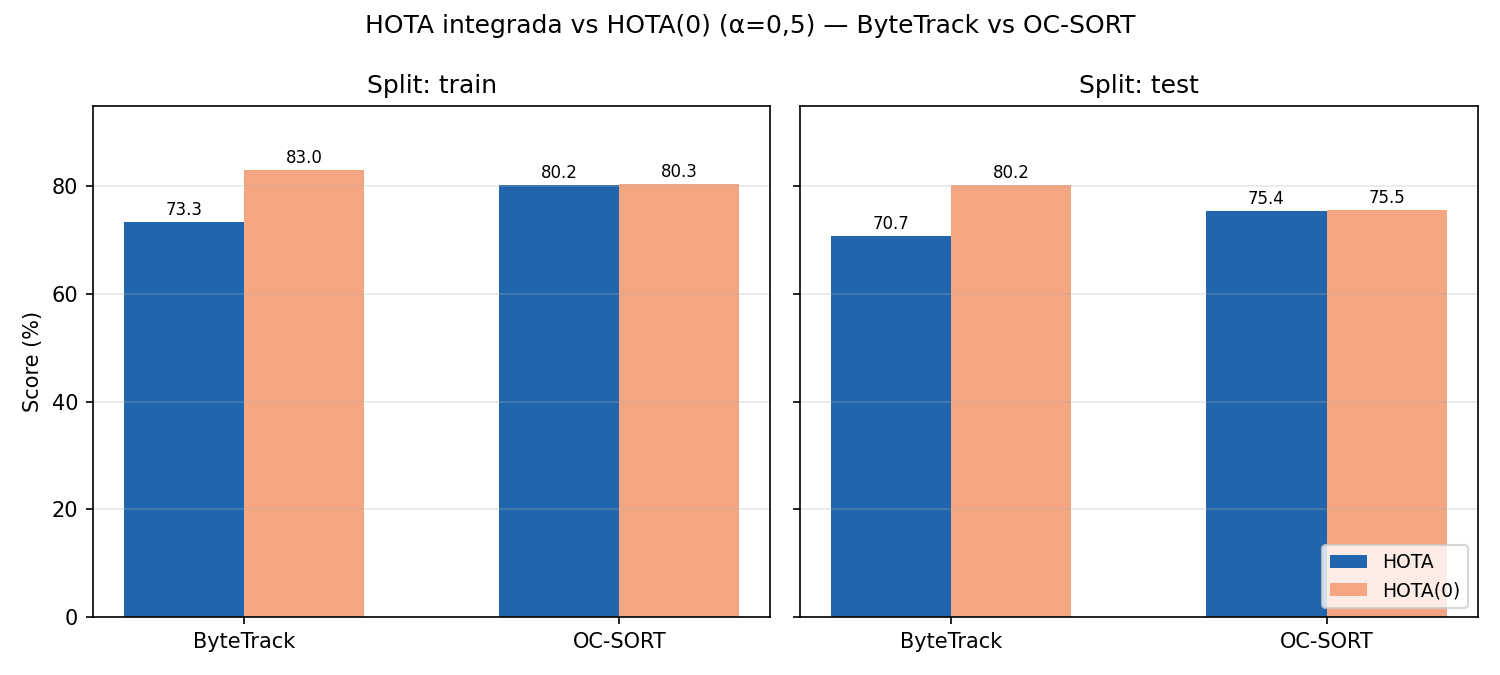
\includegraphics[width=0.92\textwidth]{figures/pruebas_hota_vs_hota0.png}
\caption{HOTA integrada frente a HOTA(0) para ambos algoritmos. Bajo HOTA
integrada, OC-SORT gana en ambos splits; bajo HOTA(0), la lectura se
invierte a favor de ByteTrack.}
\label{fig:pruebas-hota-vs-hota0}
\end{figure}

Esta discrepancia es visible en las columnas de
precisión de localización (\texttt{LocA}) del fichero
\texttt{pedestrian\_summary.txt} de \texttt{TrackEval}. OC-SORT alcanza una
\texttt{LocA} y una \texttt{DetPr} prácticamente perfectas (superiores al
99,9\,\% en ambos splits), lo que indica que \textbf{OC-SORT reutiliza
directamente las cajas del \texttt{det.txt} original sin modificarlas},
coherente con su diseño centrado en la observación. ByteTrack, en cambio, obtiene
una \texttt{LocA} sensiblemente más baja (89,8\,\% en train, 89,7\,\% en
test), lo que indica que sus cajas de salida se desvían algo más de las
detecciones originales (posiblemente por la interpolación de posición
que realiza el filtro de Kalman durante su segunda ronda de asociación con
detecciones de baja confianza (sección~\ref{subsec:fundamentos-bytetrack})).

Esa imprecisión de localización de ByteTrack apenas penaliza a HOTA(0),
calculada en un único umbral de IoU (0,5), pero se
paga cara en la HOTA integrada, que promedia también sobre umbrales mucho
más exigentes (hasta 0,95). A esos umbrales estrictos, una caja
ligeramente desplazada dejará de solapar lo suficiente con el
\emph{ground truth} para contar como acierto, mientras que las cajas casi
perfectas de OC-SORT siguen acertando. En definitiva, \textbf{ByteTrack
detecta más objetos y con más consistencia de identidad relativa
(mayor \texttt{DetRe}), pero los localiza con menos precisión. OC-SORT
detecta algo menos pero con una fidelidad casi perfecta a la detección
original}, y es esta diferencia de precisión geométrica, 
la que explica el por qué la métrica más exigente (HOTA integrada)
favorece a OC-SORT mientras que la métrica de umbral único (HOTA(0))
favorece a ByteTrack.

La conclusión que se extrae de esto y que corrige la lectura
inicial de las anotaciones de desarrollo de este proyecto, es que
\textbf{OC-SORT es el algoritmo con mejor rendimiento global en este
dataset}, tanto en entrenamiento como en test, cuando se evalúa con la
métrica íntegra y más robusta del campo. Dicho esto, ByteTrack con su menor precisión de localización es
perfectamente compatible con aplicaciones menos exigentes en exactitud
geométrica de la caja, y su comportamiento bajo ajuste de hiperparámetros
resulta, de hecho, más estable que el de OC-SORT.

\section{Resultados del estudio de hiperparámetros}
\label{sec:pruebas-hiperparametros}

El estudio de hiperparámetros se reporta en términos de HOTA(0) y no de
HOTA integrada. La Figura~\ref{fig:pruebas-hiperparametros} muestra el
efecto de los dos hiperparámetros con mayor impacto observado, uno por
algoritmo, y la Tabla~\ref{tab:pruebas-hiperparametros-sensibilidad}
recoge el análisis de sensibilidad completo sobre las configuraciones
base descritas en la sección~\ref{sec:implementacion-hiperparametros}.

\begin{figure}[htp]
\centering
\begin{minipage}{0.48\textwidth}
\centering
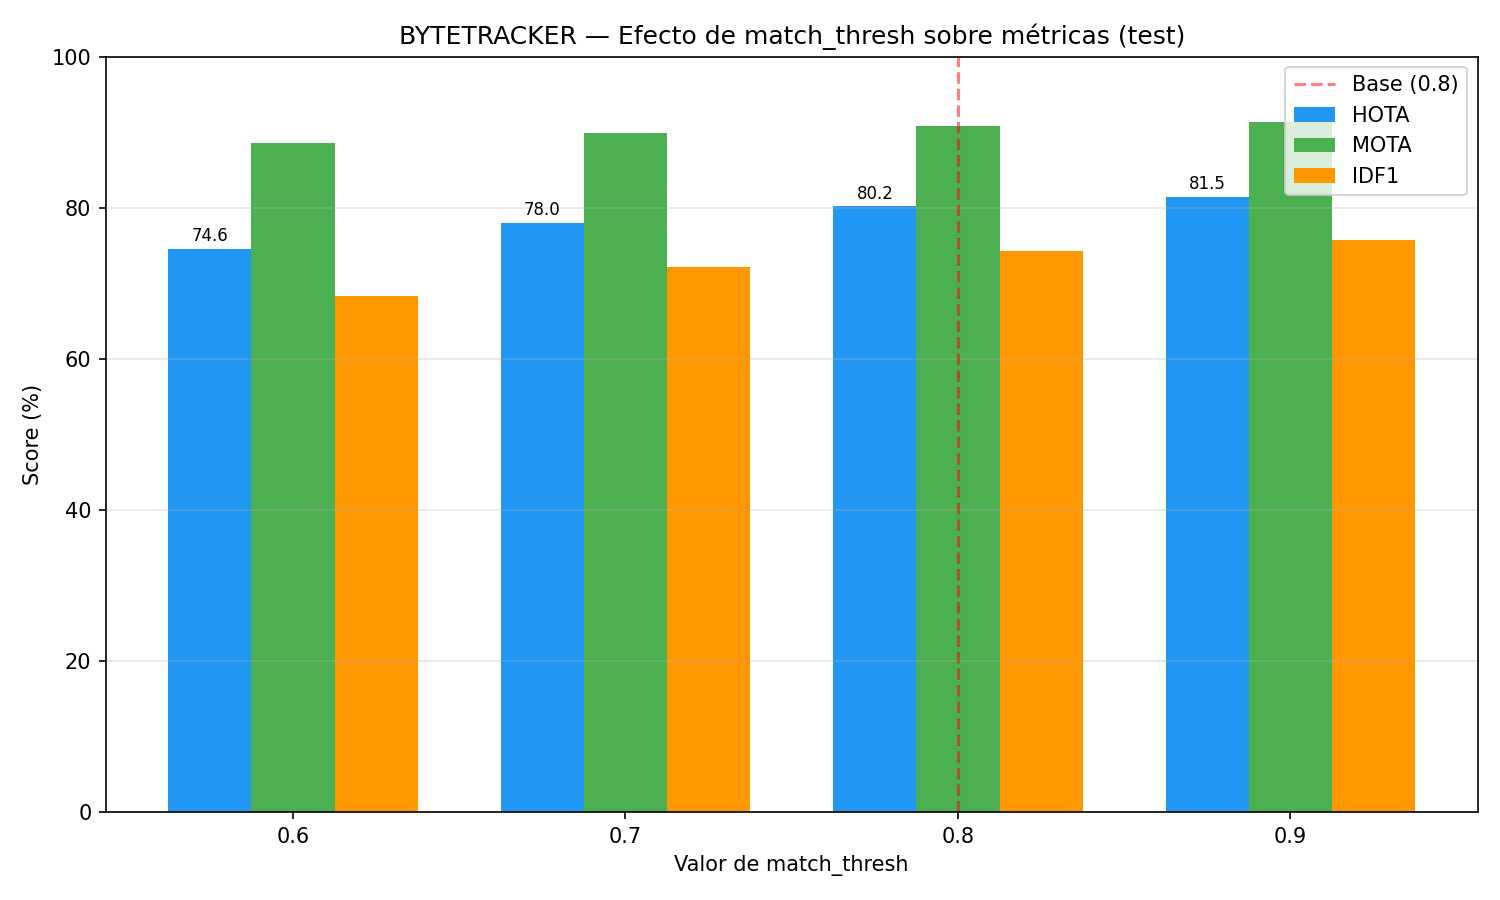
\includegraphics[width=\textwidth]{figures/pruebas_hiperparam_bytetracker.png}
\end{minipage}
\hfill
\begin{minipage}{0.48\textwidth}
\centering
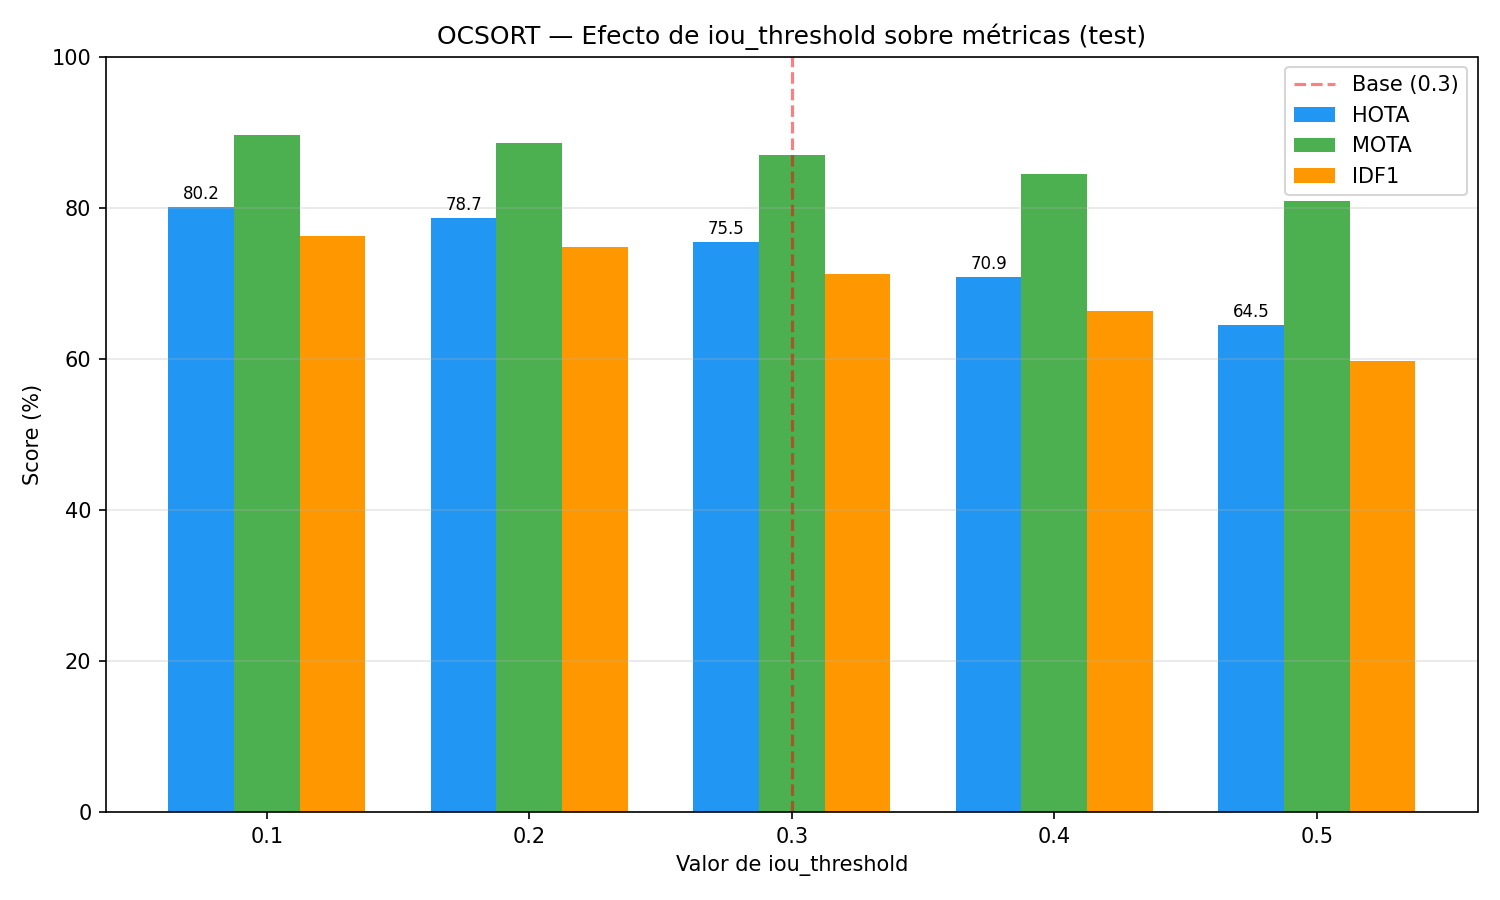
\includegraphics[width=\textwidth]{figures/pruebas_hiperparam_ocsort.png}
\end{minipage}
\caption{Efecto de \texttt{match\_thresh} sobre ByteTrack (izquierda) y de
\texttt{iou\_threshold} sobre OC-SORT (derecha), los dos hiperparámetros de
mayor impacto individual encontrados en el estudio
(sección~\ref{sec:implementacion-hiperparametros}).}
\label{fig:pruebas-hiperparametros}
\end{figure}

\FloatBarrier

\begin{table}[htp]
\centering
\caption{Análisis de sensibilidad: efecto de cada hiperparámetro sobre HOTA(0) (\%) en el conjunto de test.}
\label{tab:pruebas-hiperparametros-sensibilidad}
\renewcommand{\arraystretch}{1.2}
\small
\begin{tabular}{|p{3.1cm}|p{1.5cm}|p{1.5cm}|p{1.5cm}|p{1.5cm}|p{1.5cm}|}
\hline
\rowcolor{gray!25}
\textbf{Hiperparámetro} & \multicolumn{5}{c|}{\textbf{Valor del hiperparámetro}} \\
\hline
\texttt{match\_thresh} (BT) & 0.6 & 0.7 & 0.8 (base) & 0.9 & -- \\
\hline
HOTA(0) & 74.62 & 78.03 & 80.20 & \textbf{81.48} & -- \\
\hline
\texttt{track\_buffer} (BT) & 10 & 20 & 25 (base) & 40 & -- \\
\hline
HOTA(0) & \textbf{80.36} & 80.26 & 80.20 & 80.12 & -- \\
\hline
\texttt{iou\_threshold} (OC) & 0.1 & 0.2 & 0.3 (base) & 0.4 & 0.5 \\
\hline
HOTA(0) & \textbf{80.17} & 78.71 & 75.51 & 70.90 & 64.49 \\
\hline
\texttt{max\_age} (OC) & 10 & 20 & 30 (base) & 50 & -- \\
\hline
HOTA(0) & \textbf{76.13} & 75.75 & 75.51 & 75.13 & -- \\
\hline
\texttt{min\_hits} (OC) & 1 & 2 & 3 (base) & 5 & -- \\
\hline
HOTA(0) & \textbf{76.26} & 75.90 & 75.51 & 74.78 & -- \\
\hline
\end{tabular}
\end{table}

\FloatBarrier

El resultado más relevante de este estudio es que \textbf{el ajuste
de hiperparámetros beneficia mucho más a OC-SORT que a ByteTrack}: OC-SORT
mejora su HOTA(0) en test de 75,51 a 80,92 (+5,41 puntos) con la
configuración óptima combinada, mientras que ByteTrack mejora de 80,20 a
81,43 (+1,23 puntos). Dicho de otro modo, ByteTrack ya operaba cerca de su
óptimo con los valores por defecto, mientras que OC-SORT
requería un ajuste explícito para desplegar todo su rendimiento. Esta
observación es coherente con la comparativa de la
sección~\ref{sec:pruebas-comparativa}: si se repitiera la comparación de
HOTA integrada usando las configuraciones óptimas de ambos algoritmos en
lugar de sus valores por defecto, es razonable esperar que la ventaja de
OC-SORT sobre ByteTrack se mantenga o incluso se ampliase, dado que es
OC-SORT quien más partido saca del ajuste.

Es interesante notar que la configuración combinada de ByteTrack
(81{,}43) resulta ligeramente \emph{inferior} al mejor valor individual de
\texttt{match\_thresh} por sí solo (81{,}48 con
\texttt{match\_thresh=0.9} y \texttt{track\_buffer} sin modificar): los
efectos de ambos hiperparámetros no son estrictamente aditivos, y combinar
el mejor valor de cada uno por separado no garantiza el mejor resultado
conjunto. En OC-SORT, en cambio, la combinación de los tres
hiperparámetros (80{,}92) mejora claramente sobre cualquiera de ellos por
separado (mejor individual: 80{,}17 con \texttt{iou\_threshold=0.1}), lo
que indica que en este caso sí se refuerzan entre sí.

Por ser la configuración de mayor HOTA(0) absoluto entre las dos
configuraciones óptimas (81,43 frente a 80,92), \textbf{ByteTrack con
\texttt{match\_thresh=0.9} y \texttt{track\_buffer=10}} es la que se ha
usado como base de todo el pipeline de metadatos de la siguiente sección,
una decisión tomada en su momento con la información de HOTA(0) disponible
entonces.

\section{Resultados del pipeline de metadatos}
\label{sec:pruebas-metadatos}

Esta sección presenta los resultados del pipeline de metadatos sobre las secuencias de
demostración SNMOT-116, SNMOT-117 y SNMOT-118, obtenidos sobre la
configuración óptima de ByteTrack.

\subsection{Clasificación de equipos}

La Tabla~\ref{tab:pruebas-equipos} resume el resultado de la clasificación
de equipos por K-means (sección~\ref{subsec:impl-equipos}) sobre las tres
secuencias de demostración.

\begin{table}[htp]
\centering
\caption{Resultado de la clasificación de equipos por secuencia.}
\label{tab:pruebas-equipos}
\renewcommand{\arraystretch}{1.25}
\begin{tabular}{|p{2.2cm}|p{2.2cm}|p{2.2cm}|p{2.2cm}|}
\hline
\rowcolor{gray!25}
\textbf{Secuencia} & \textbf{Jugadores clasificados} & \textbf{Equipo 0} & \textbf{Equipo 1} \\
\hline
SNMOT-116 & 61 & 29 & 32 \\
\hline
SNMOT-117 & 46 & 16 & 30 \\
\hline
SNMOT-118 & 44 & 24 & 20 \\
\hline
\end{tabular}
\end{table}

\FloatBarrier

La verificación visual (\texttt{team\_visualization.py}) confirma que la
separación por color de camiseta funciona correctamente para los
jugadores de ambos equipos en las tres secuencias, como muestra la
Figura~\ref{fig:pruebas-teams}. Como se documentó en la
sección~\ref{sec:fundamentos-kmeans}, ningún \texttt{track\_id} queda
etiquetado como ``árbitro'': con $k=2$, el árbitro presente en la secuencia
se asigna incorrectamente al equipo de color más cercano al de su
uniforme, una limitación conocida.

\begin{figure}[htp]
\centering
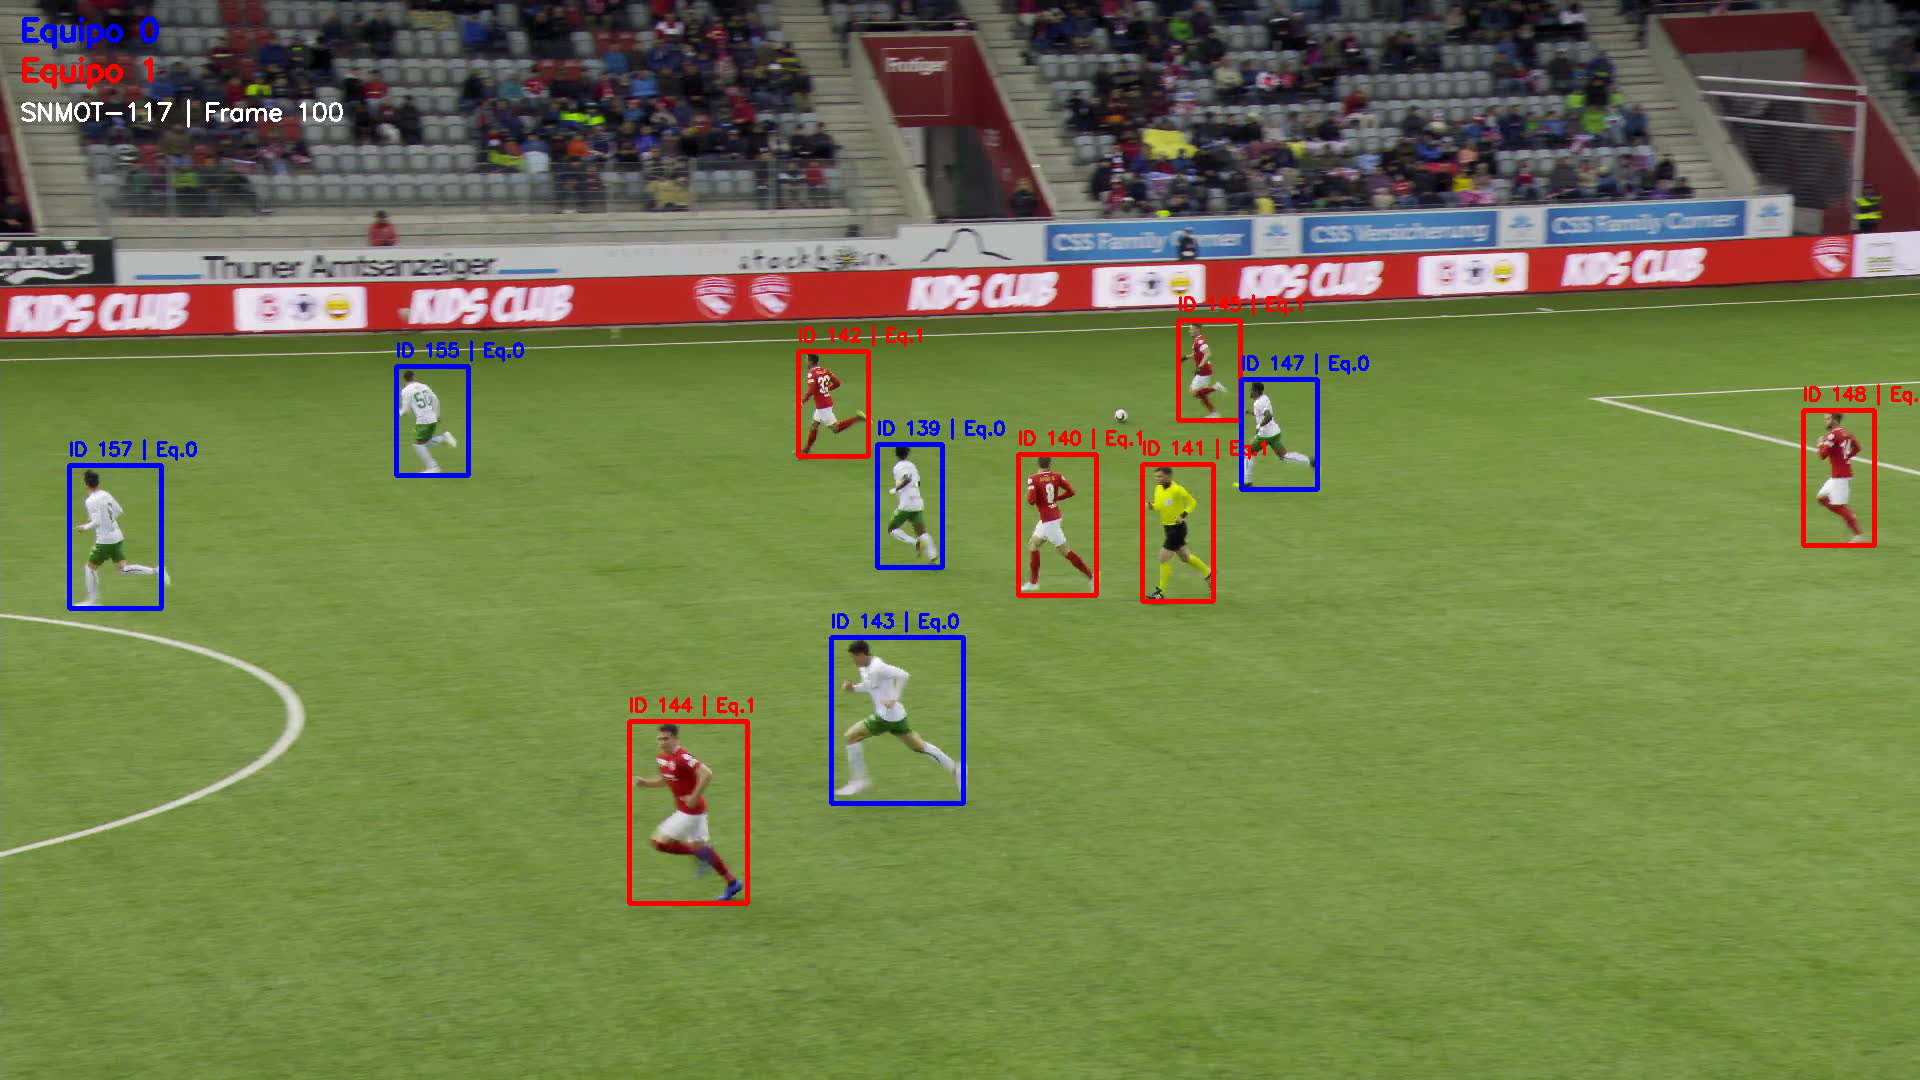
\includegraphics[width=0.85\textwidth]{figures/pruebas_teams_ejemplo.png}
\caption{Clasificación de equipos sobre un frame de
SNMOT-117 (\texttt{team\_visualization.py}).}
\label{fig:pruebas-teams}
\end{figure}

\FloatBarrier

\subsection{Mapas de calor}

La Figura~\ref{fig:pruebas-heatmap} muestra el mapa de calor general
sin homografía, con la proyección aproximada por rango observado
de SNMOT-116, complementario al
mapa de calor por equipo de SNMOT-117 ya mostrado en la
Figura~\ref{fig:diseno-heatmap-ejemplo} del capítulo~\ref{cap:diseno}.

\begin{figure}[htp]
\centering
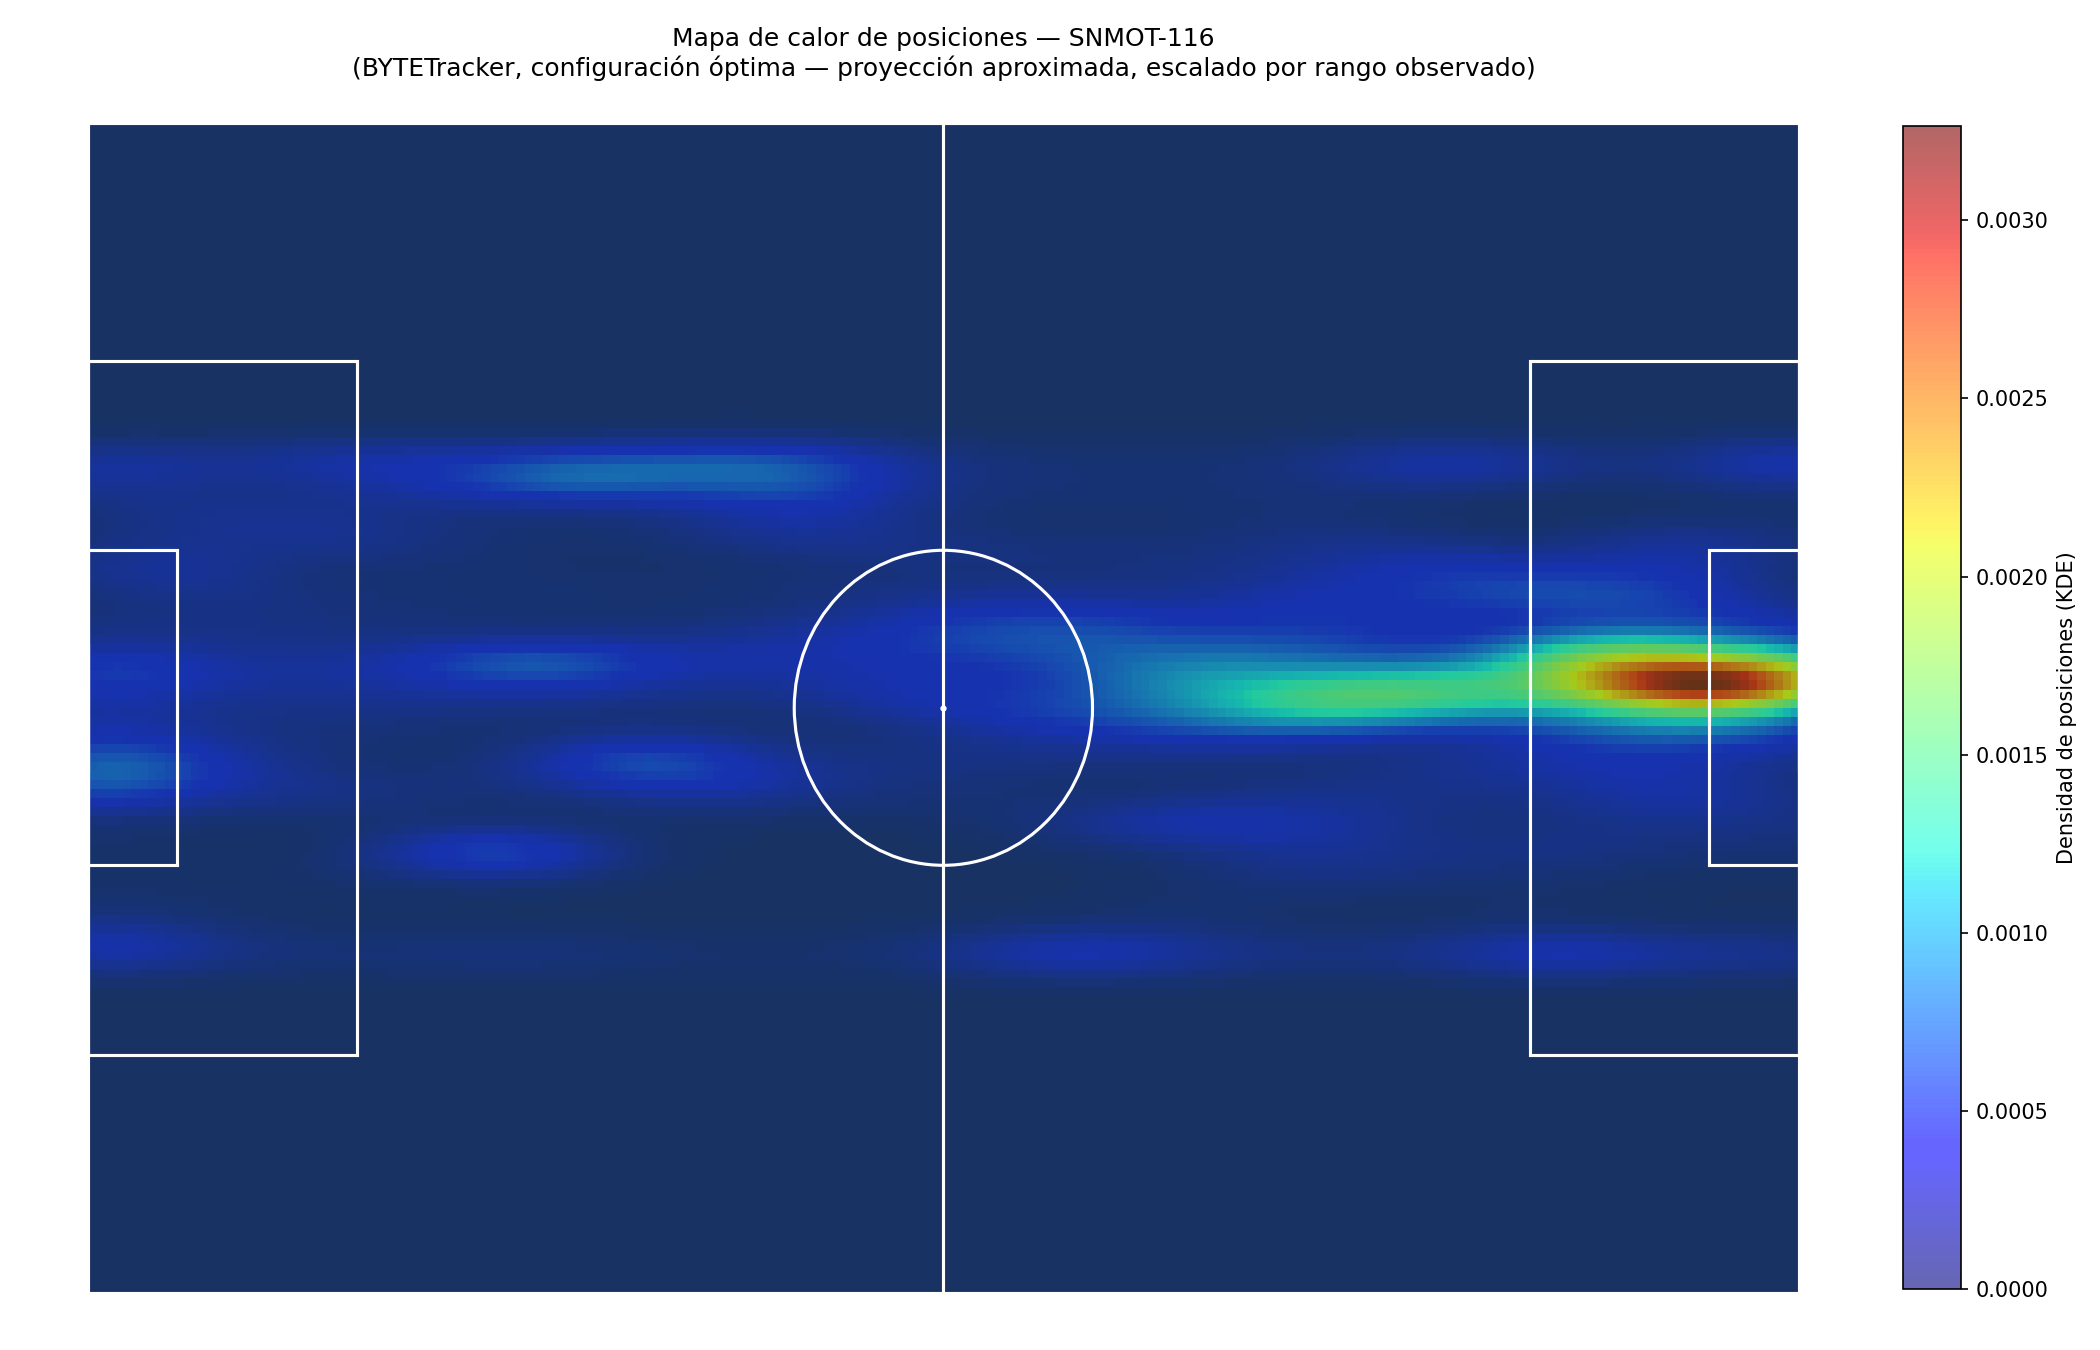
\includegraphics[width=0.85\textwidth]{figures/pruebas_heatmap_field_ejemplo.png}
\caption{Mapa de calor general de SNMOT-116, proyección aproximada sin
homografía.}
\label{fig:pruebas-heatmap}
\end{figure}

\FloatBarrier

\subsection{Distancia y velocidad por homografía}

La Tabla~\ref{tab:pruebas-distancia} recoge los cinco jugadores con mayor
distancia recorrida en cada uno de los dos tramos de demostración
analizados con homografía real.

\begin{table}[htp]
\centering
\caption{Jugadores con mayor distancia recorrida en cada tramo analizado con homografía real.}
\label{tab:pruebas-distancia}
\renewcommand{\arraystretch}{1.25}
\begin{tabular}{|p{2.3cm}|p{1.6cm}|p{2.2cm}|p{2.4cm}|p{2.4cm}|}
\hline
\rowcolor{gray!25}
\textbf{Secuencia} & \textbf{ID} & \textbf{Distancia (m)} & \textbf{Vel.\ media (km/h)} & \textbf{Vel.\ pico p95 (km/h)} \\
\hline
\multirow{5}{*}{SNMOT-116} & 14 & 46{,}81 & 7{,}12 & 21{,}23 \\
\cline{2-5}
 & 13 & 45{,}06 & 7{,}67 & 17{,}42 \\
\cline{2-5}
 & 11 & 41{,}12 & 6{,}46 & 18{,}83 \\
\cline{2-5}
 & 9 & 41{,}07 & 8{,}15 & 17{,}63 \\
\cline{2-5}
 & 8 & 40{,}55 & 7{,}34 & 16{,}73 \\
\hline
\multirow{5}{*}{SNMOT-118} & 279 & 48{,}07 & 12{,}92 & 28{,}76 \\
\cline{2-5}
 & 273 & 33{,}03 & 8{,}68 & 28{,}11 \\
\cline{2-5}
 & 309 & 23{,}18 & 7{,}55 & 13{,}50 \\
\cline{2-5}
 & 335 & 22{,}82 & 6{,}53 & 12{,}16 \\
\cline{2-5}
 & 271 & 22{,}77 & 5{,}67 & 10{,}58 \\
\hline
\end{tabular}
\end{table}

\FloatBarrier

Las magnitudes resultan físicamente plausibles para tramos tan cortos: 25 y
16 jugadores rastreados respectivamente en cada tramo (todos los
\texttt{track\_id} con posiciones dentro de la ventana analizada), con
distancias de hasta 48\,m y velocidades de pico de hasta 28{,}8\,km/h en el
tramo de SNMOT-118, coherentes con un sprint corto durante una jugada
ofensiva. La Figura~\ref{fig:pruebas-heatmap-homografia} muestra el mapa de
calor con homografía real de SNMOT-118, complementario al de SNMOT-116 ya
mostrado en la Figura~\ref{fig:diseno-heatmap-homografia-ejemplo}.

\begin{figure}[htp]
\centering
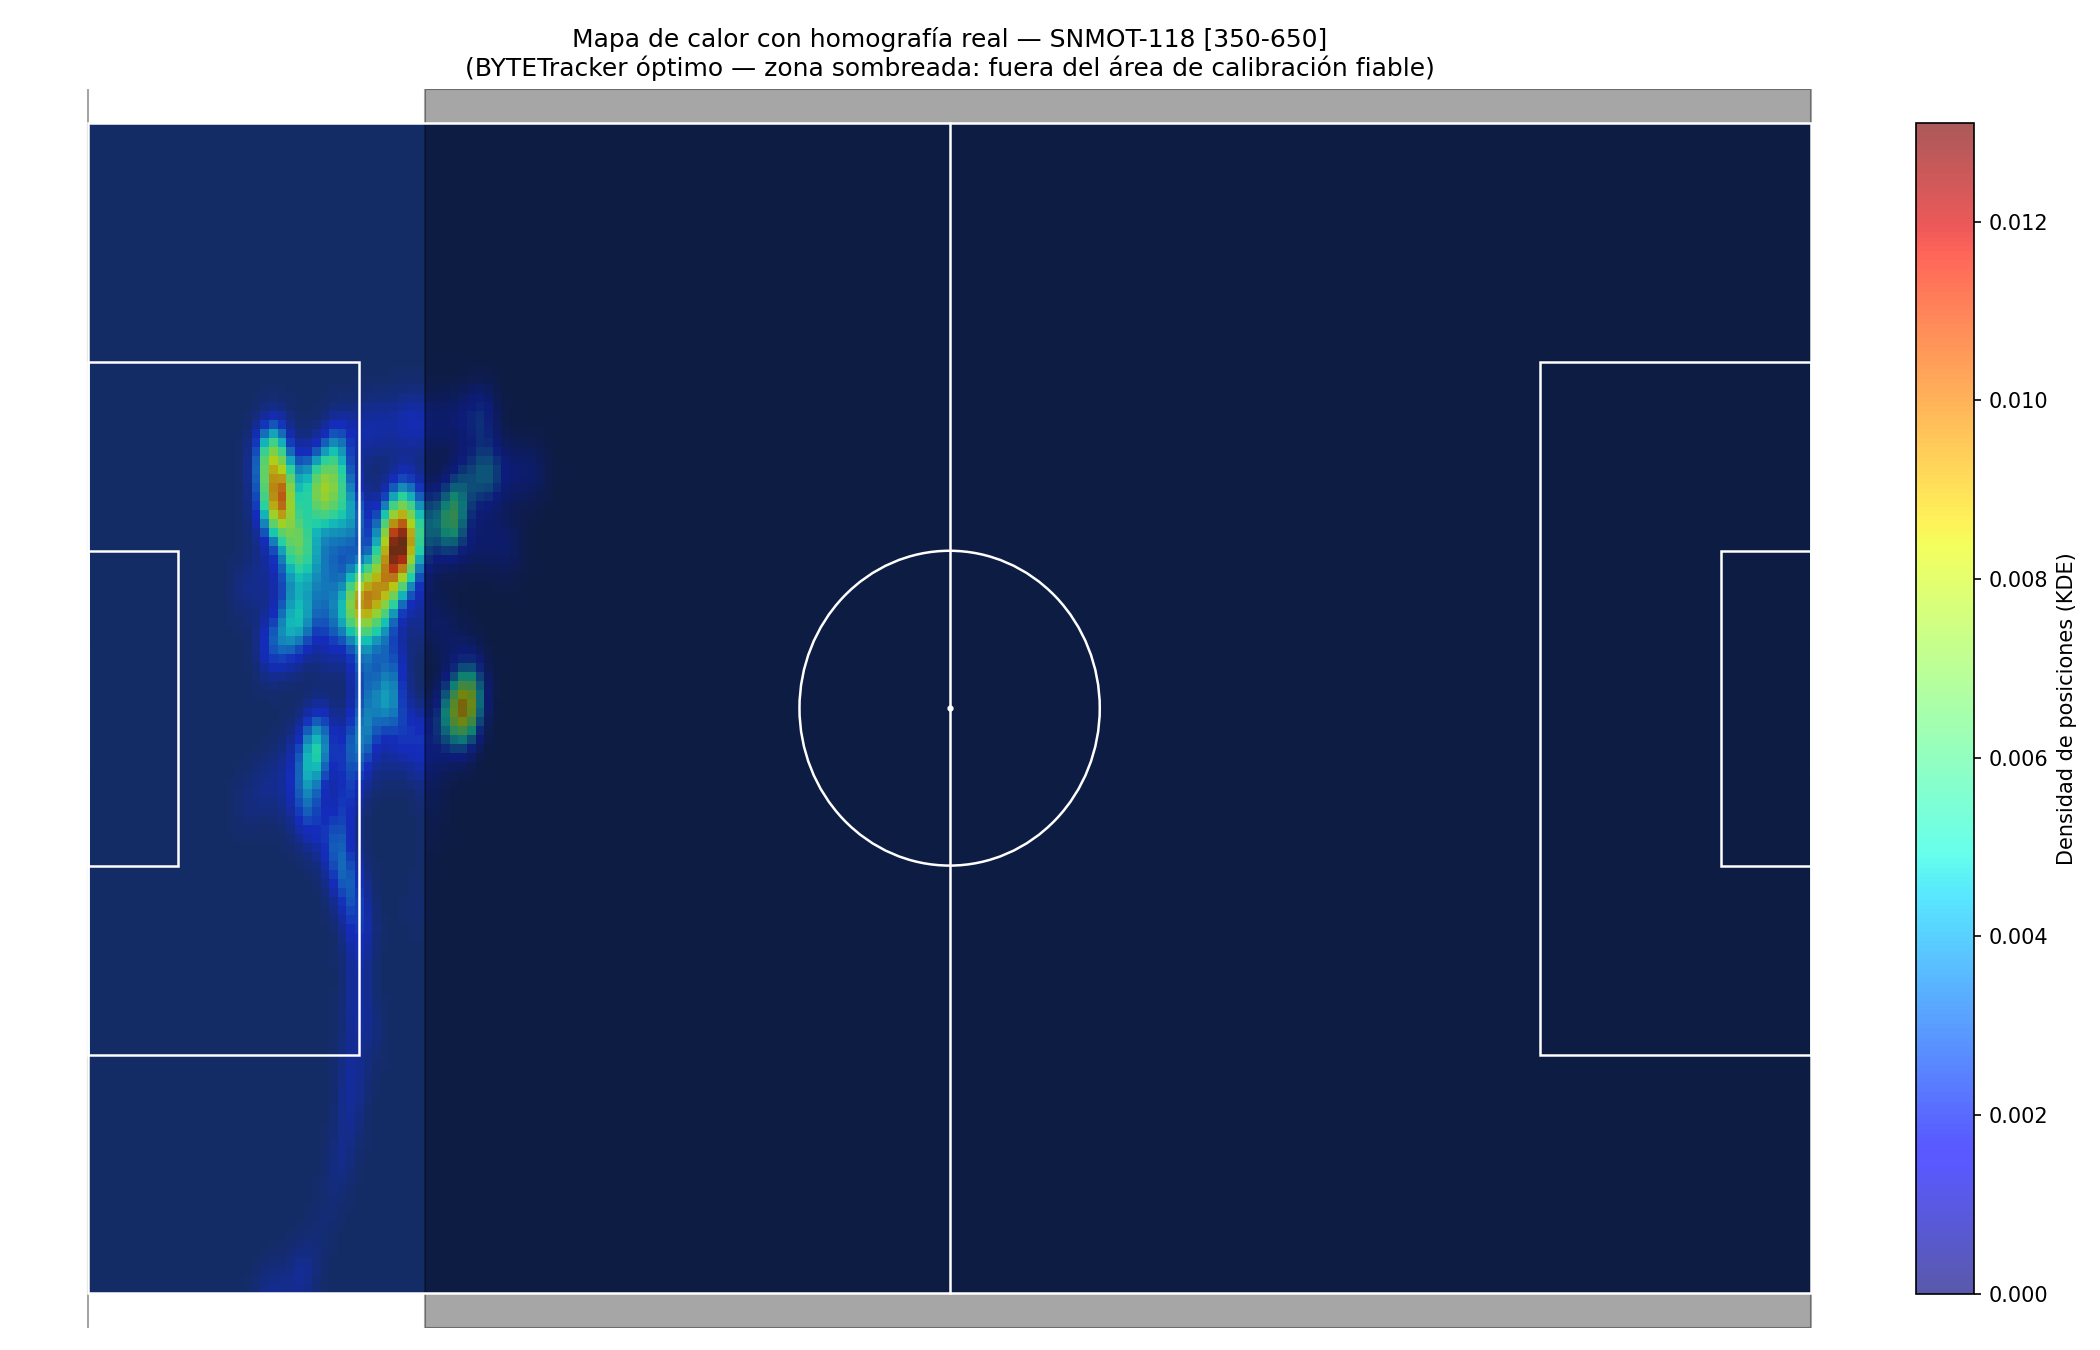
\includegraphics[width=0.85\textwidth]{figures/pruebas_heatmap_homografia_ejemplo.png}
\caption{Mapa de calor con homografía real sobre el tramo de SNMOT-118; la
zona sombreada indica dónde la calibración no es fiable.}
\label{fig:pruebas-heatmap-homografia}
\end{figure}

\FloatBarrier

\subsection{Posesión de balón}

La Tabla~\ref{tab:pruebas-posesion} recoge el porcentaje de posesión por
equipo, estimado por proximidad espacial, en las tres secuencias de
demostración.

\begin{table}[htp]
\centering
\caption{Posesión de balón por equipo y secuencia (estimada por proximidad).}
\label{tab:pruebas-posesion}
\renewcommand{\arraystretch}{1.25}
\begin{tabular}{|p{2.4cm}|p{2.6cm}|p{2.6cm}|p{2.6cm}|}
\hline
\rowcolor{gray!25}
\textbf{Secuencia} & \textbf{Equipo 0} & \textbf{Equipo 1} & \textbf{Frames con posesión asignada} \\
\hline
SNMOT-116 & 85{,}95\,\% & 14{,}05\,\% & 612 \\
\hline
SNMOT-117 & 71{,}81\,\% & 28{,}19\,\% & 667 \\
\hline
SNMOT-118 & 25{,}06\,\% & 74{,}94\,\% & 427 \\
\hline
\end{tabular}
\end{table}

Los repartos obtenidos varían considerablemente de una secuencia a otra
, lo que es consistente con tratarse de tramos
cortos de partido en los que un equipo puede
dominar claramente la posesión del balón durante una jugada concreta sin
que eso sea representativo de la posesión a lo largo de todo el partido.
Como se documentó en el diseño de esta métrica
(sección~\ref{subsec:diseno-posesion}), estos porcentajes deben leerse como
lo que son, una aproximación por proximidad espacial frame a frame y no como una estadística oficial de
partido.

\section{Limitaciones de los resultados}
\label{sec:pruebas-limitaciones}

Al igual que en el resto de esta memoria, conviene cerrar este capítulo
resumiendo las limitaciones que afectan a la validez de
los resultados presentados:

\begin{itemize}
  \item \textbf{HOTA(0) frente a HOTA integrada}: el estudio de
        hiperparámetros completo
        se reporta en términos de HOTA(0), no de la métrica integrada más
        robusta usada en la comparativa principal
        . Recalcular el estudio
        completo con HOTA integrada queda
        como trabajo futuro.
  \item \textbf{Configuraciones óptimas no recombinadas}: no se ha vuelto a
        evaluar la comparativa de HOTA integrada de la
        sección~\ref{sec:pruebas-comparativa} usando las configuraciones
        óptimas de hiperparámetros de cada algoritmo, solo sus valores por
        defecto.
  \item \textbf{Clasificación de equipos sin árbitro}: los porcentajes de
        posesión y los mapas de calor por equipo incluyen al árbitro
        clasificado incorrectamente en uno de los dos equipos, lo que introduce un sesgo
        pequeño en ambos resultados.
  \item \textbf{Homografía real limitada a dos tramos cortos}: los
        resultados de distancia y velocidad se basan en 12-15 segundos de
        vídeo de dos secuencias concretas, no en partidos completos.
  \item \textbf{Posesión como heurística}: los
        porcentajes de la Tabla~\ref{tab:pruebas-posesion} miden proximidad
        espacial al balón, no posesión táctica real, y se calculan sobre
        secuencias muy cortas.
  \item \textbf{Detección del balón por criterio geométrico}: cualquier
        resultado que dependa de la localización del balón tendría
        las limitaciones del filtro geométrico.
\end{itemize}

    \chapter{Manual de despliegue}
\label{cap:manual}

Este capítulo describe cómo instalar, configurar y ejecutar el sistema, qué
artefactos produce cada script y cómo interpretar los resultados. Este capítulo es una guía práctica de uso
paso a paso, pensada para que cualquier persona con el dataset descargado
pueda reproducir los resultados de esta memoria.

\section{Requisitos previos}
\label{sec:manual-requisitos}

La Tabla~\ref{tab:manual-requisitos} resume el software necesario para
ejecutar tanto el pipeline offline en Python como la aplicación web. El
proyecto se ha desarrollado y probado en Windows y macOS
(sección~\ref{sec:gestion-entorno}), sin dependencias específicas de
sistema operativo más allá de las propias de Python y Node.js.

\begin{table}[htp]
\centering
\caption{Requisitos previos para desplegar el sistema completo.}
\label{tab:manual-requisitos}
\renewcommand{\arraystretch}{1.25}
\begin{tabular}{|p{3.4cm}|p{9.4cm}|}
\hline
\rowcolor{gray!25}
\textbf{Requisito} & \textbf{Detalle} \\
\hline
Python & 3.11: versiones más recientes de Python no son
  compatibles con las versiones de las librerías usadas en este proyecto. \\
\hline
Node.js & 18 o superior, con \texttt{npm} incluido (necesario solo para la
  aplicación web). \\
\hline
Git & Cualquier versión reciente, para clonar el repositorio. \\
\hline
Espacio en disco & Al menos 60\,GB libres: el conjunto completo de la tarea
  \texttt{tracking} de SoccerNet (\emph{splits} train, test y challenge)
  ocupa unos 55\,GB una vez descomprimido. \\
\hline
Conexión a internet & Estable y sin límite de datos ajustado durante la
  descarga inicial del dataset, dado
  su tamaño. \\
\hline
\end{tabular}
\end{table}

No se requiere GPU: los algoritmos de tracking usados (ByteTrack, OC-SORT)
son clásicos y todo el pipeline se ha ejecutado sobre CPU sin que ello
supusiera una limitación relevante (sección~\ref{sec:gestion-entorno}).

\section{Instalación}
\label{sec:manual-instalacion}

\subsection{Obtención del código}

El código fuente está alojado en el repositorio de GitHub del proyecto:

\begin{lstlisting}[language=bash]
git clone https://github.com/cgaleam/Soccernet-Tracking-Analysis.git
cd Soccernet-Tracking-Analysis
\end{lstlisting}

Todas las rutas relativas del pipeline (\texttt{../SoccerNet/...}, usadas de
forma consistente en los scripts de \texttt{src/}) asumen que el dataset se
descarga como una carpeta hermana del repositorio, no dentro de él.

\subsection{Entorno Python}
\label{subsec:manual-venv}

El proyecto usa un entorno virtual estándar de Python, no \texttt{conda}
(problema P2, Tabla~\ref{tab:impl-problemas}):

\begin{lstlisting}[language=bash]
python3.11 -m venv venv_tfg

# macOS / Linux
source venv_tfg/bin/activate

# Windows (PowerShell)
venv_tfg\Scripts\Activate.ps1

pip install -r requirements.txt
\end{lstlisting}

\texttt{requirements.txt} fija las versiones exactas de todas las
dependencias, incluyendo \texttt{numpy==2.4.4}, \texttt{boxmot==10.0.43} y
\texttt{opencv-python==4.13.0.92}
. Existe una inconsistencia
conocida y documentada, \texttt{trackeval} no aparece listado explícitamente en
\texttt{requirements.txt} aunque el resto del pipeline lo importa
directamente. Si \texttt{pip install -r requirements.txt} no lo instala
como dependencia de otro paquete, instalarlo aparte con
\texttt{pip install trackeval}.

\subsection{Descarga del dataset SoccerNet}
\label{subsec:manual-dataset}

La descarga se realiza con el SDK oficial de SoccerNet, incluido en
\texttt{requirements.txt}:

\begin{lstlisting}[language=bash]
python src/utils/soccernet_download.py
\end{lstlisting}

Este script descarga los \emph{splits} train, test y challenge de las
tareas \texttt{tracking} y \texttt{tracking-2023} en una carpeta
\texttt{SoccerNet/} creada en paralelo al repositorio, reproduciendo la estructura
\texttt{SoccerNet/tracking/\{train,test,challenge\}/SNMOT-XXX/} que
consumen el resto de scripts del proyecto. A diferencia de otras tareas del
ecosistema SoccerNet que exigen solicitar acceso mediante un formulario
NDA (por ejemplo, los vídeos completos de partido), la tarea
\texttt{tracking} se descarga con una contraseña genérica de acceso
público, incluida en el propio SDK, sin gestión adicional por parte
del usuario. En la ejecución realizada durante este proyecto, la tarea
\texttt{tracking-2023} no llegó a descargar ningún dato (el propio SDK
informa de que ese \emph{split} concreto no estaba disponible en el
servidor en ese momento), sin que ello afecte al resto del pipeline, que
usa exclusivamente la tarea \texttt{tracking}.

\section{Estructura del repositorio}
\label{sec:manual-estructura}

La Tabla~\ref{tab:impl-estructura}
detalla la responsabilidad de cada paquete de \texttt{src/}. A efectos
prácticos de navegación, el árbol de directorios relevante tras completar
la instalación y una primera ejecución completa es el siguiente:

\begin{lstlisting}[language=bash]
Soccernet-Tracking-Analysis/
  src/
    visualizacion/        # scripts exploratorios iniciales
    tracking/             # ByteTrack, OC-SORT, ejecucion batch, export de video
    evaluation/           # seqmaps + evaluacion con TrackEval
    hyperparameter_study/
    metadata/             # equipos, heatmaps, homografia, posesion
    web_export/           # metadatos de OC-SORT + paquete de datos para la web
    utils/
  frontend/                # aplicacion web
  results_train/, results_test/          # .txt de tracking por secuencia
  results_hyperparam/                    # resultados del barrido + configuraciones optimas
  evaluation_train/, evaluation_test/    # salida de TrackEval
  evaluation_hyperparam/                 # resumen + graficas del estudio de hiperparametros
  metadata_output/                       # equipos, heatmaps, homografia, posesion
  videos/                                # videos anotados exportados
  memoria/                               # este documento
  requirements.txt
  venv_tfg/                              # entorno virtual
\end{lstlisting}

\texttt{results\_train/}, \texttt{evaluation\_train/} y el resto de
carpetas de salida no se incluyen en el repositorio: las genera cada script
la primera vez que se ejecuta.

\section{Ejecución del pipeline de tracking}
\label{sec:manual-tracking}

Los scripts de \texttt{src/tracking/} cubren dos casos de uso distintos:
explorar una única secuencia con un algoritmo concreto, o procesar un
\emph{split} completo con ambos algoritmos (sección~\ref{sec:implementacion-tracking}).

Para explorar una única secuencia, \texttt{bytetracker\_alg.py} y
\texttt{sort\_alg.py} no aceptan argumentos
de línea de comandos: la secuencia a procesar se fija editando la variable
\texttt{base\_path} al principio del fichero antes de ejecutarlo.

\begin{lstlisting}[language=bash]
# Editar antes de ejecutar: base_path = "../SoccerNet/tracking/train/SNMOT-XXX/"
python src/tracking/bytetracker_alg.py
python src/tracking/sort_alg.py
\end{lstlisting}

Para reproducir los resultados de esta memoria, el flujo real es la
ejecución batch sobre el \emph{split} completo, que sí recorre todas las
secuencias automáticamente:

\begin{lstlisting}[language=bash]
python src/tracking/run_all_train.py   # -> results_train/{bytetracker,ocsort}/
python src/tracking/run_all_test.py    # -> results_test/{bytetracker,ocsort}/
\end{lstlisting}

Cada ejecución tarda del orden de varias horas sobre CPU, al procesar las
57 secuencias de train o las 49 de test con ambos algoritmos
frame a frame. Para exportar un vídeo anotado de una secuencia concreta
(por defecto, SNMOT-076 de train):

\begin{lstlisting}[language=bash]
python src/tracking/export/export_bytetracker.py   # -> videos/SNMOT-076_bytetracker.mp4
python src/tracking/export/export_sort.py           # -> videos/SNMOT-076_ocsort.mp4
\end{lstlisting}

\section{Ejecución de la evaluación}
\label{sec:manual-evaluacion}

\texttt{TrackEval} necesita un fichero \emph{seqmap} que le indique qué
secuencias evaluar, que debe generarse antes de la evaluación propiamente
dicha:

\begin{lstlisting}[language=bash]
python src/evaluation/seqmpas_creation_train.py
python src/evaluation/seqmaps_creation_test.py
python src/evaluation/evaluate_train.py   # -> evaluation_train/
python src/evaluation/evaluate_test.py    # -> evaluation_test/
\end{lstlisting}

Cada carpeta de salida contiene, por algoritmo y secuencia, un
\texttt{pedestrian\_summary.txt} con las columnas de HOTA, HOTA(0), DetA,
AssA, MOTA e IDF1 usadas en la comparativa del
capítulo~\ref{cap:pruebas}.

\section{Ejecución del estudio de hiperparámetros}
\label{sec:manual-hiperparametros}

\begin{lstlisting}[language=bash]
python src/hyperparameter_study/hyperparam_bytetracker.py  # -> results_hyperparam/bytetracker/
python src/hyperparameter_study/hyperparam_ocsort.py       # -> results_hyperparam/ocsort/
python src/hyperparameter_study/summarize_hyperparam.py    # -> evaluation_hyperparam/summary_table.csv y /plots/
python src/hyperparameter_study/bytetracker_optimal.py     # -> results_hyperparam/bytetracker/bytetracker_optimal/
python src/hyperparameter_study/ocsort_optimal.py          # -> results_hyperparam/ocsort_optimal/
\end{lstlisting}

Los dos primeros scripts varían un hiperparámetro a la vez sobre el
\emph{split} de test, manteniendo el resto en su valor base
(sección~\ref{sec:implementacion-hiperparametros}); cada barrido completo
tarda igualmente del orden de horas. \texttt{summarize\_hyperparam.py} debe
ejecutarse después de ambos barridos, ya que lee sus resultados y produce
la tabla y las gráficas comparativas reutilizadas en el
capítulo~\ref{cap:pruebas}. Los dos últimos scripts no forman parte del
barrido: ejecutan y evalúan cada algoritmo una única vez con la
configuración óptima ya determinada, y son los que alimentan tanto el
pipeline de metadatos como la aplicación web.

\section{Ejecución del pipeline de metadatos}
\label{sec:manual-metadatos}

Todos los scripts de \texttt{src/metadata/} parten de
\texttt{results\_hyperparam/bytetracker/bytetracker\_optimal/}
 y deben ejecutarse en este
orden, ya que la clasificación de equipos es una dependencia de los
mapas de calor por equipo y de la posesión:

\begin{lstlisting}[language=bash]
python src/metadata/team_classification.py       # -> metadata_output/teams/*_teams_final.csv
python src/metadata/team_visualization.py         # -> metadata_output/teams/*_frame*.png
python src/metadata/heatmap_field.py               # -> metadata_output/heatmaps/*_heatmap_field.png
python src/metadata/heatmap_by_team.py             # -> metadata_output/heatmaps/*_heatmap_by_team.png
python src/metadata/distance_homography_demo_116.py
python src/metadata/distance_homography_demo_118.py
python src/metadata/heatmap_homography_demo_116.py
python src/metadata/heatmap_homography_demo_118.py
python src/metadata/ball_possesion.py              # -> metadata_output/possession/
\end{lstlisting}

\texttt{general\_heatmap.py} es la primera versión del mapa de calor
general y se
conserva en el repositorio a título documental, pero no forma parte del
flujo actual: \texttt{heatmap\_field.py} la sustituye por completo.
\texttt{distance\_homography\_demo\_*.py} y
\texttt{heatmap\_homography\_demo\_*.py} solo existen para SNMOT-116 y
SNMOT-118, las dos secuencias con calibración de homografía manual.

Para generar el mismo conjunto de metadatos sobre la configuración óptima
de OC-SORT, necesario para el selector de algoritmo de la aplicación
web, no para el pipeline principal, que solo usa ByteTrack, el paquete
\texttt{src/web\_export/} reproduce esta misma lógica parametrizada por
algoritmo en lugar de duplicar cada
script.


\section{Manual de la aplicación web}
\label{sec:manual-web}

\subsection{Generación del paquete de datos}

La aplicación web no recalcula nada: consume un paquete de artefactos
estáticos que debe
generarse antes de arrancarla, una vez completados los pasos anteriores
para ambos algoritmos:

\begin{lstlisting}[language=bash]
python -m src.web_export.export_bundle
# -> frontend/public/data/{videos,images}/, sequences.json, global_metrics.json
\end{lstlisting}

Este paso reescribe por completo la carpeta \texttt{frontend/public/data/} y debe repetirse cada vez que
cambien los resultados de tracking, evaluación o metadatos que consume.

\subsection{Instalación y ejecución del frontend}

\begin{lstlisting}[language=bash]
cd frontend
npm install

npm run dev      # servidor de desarrollo, http://localhost:5173
npm run build     # build estatico
npm run preview   # sirve el build de dist/ en local para verificarlo
\end{lstlisting}

\texttt{npm run dev} recarga automáticamente al editar el código de
\texttt{frontend/src/}, pero no vigila \texttt{frontend/public/data/}: si
se regenera el paquete de datos con \texttt{export\_bundle.py} mientras el
servidor de desarrollo está en marcha, hay que reiniciarlo para que recoja
los ficheros nuevos. El build de producción
(\texttt{npm run build}) genera un sitio completamente estático en
\texttt{frontend/dist/}, con rutas relativas
(\texttt{base: './'} en \texttt{vite.config.ts}), desplegable en cualquier
alojamiento estático o servible directamente en local.

\subsection{Uso de la interfaz}
\label{subsec:manual-uso-interfaz}

La aplicación se organiza en dos pestañas,
pensadas para responder dos preguntas distintas: \enquote{¿qué algoritmo
rinde mejor en general?} y \enquote{¿qué ha pasado exactamente en esta
secuencia concreta?}. Las Figuras~\ref{fig:manual-web-comparativa}
a~\ref{fig:manual-web-118} son capturas reales de la aplicación en
ejecución sobre el paquete de datos descrito en la
sección~\ref{subsec:impl-web-bundle}, y se usan a continuación para
detallar, panel a panel, qué permite consultar cada pestaña.

\paragraph{Comparativa de algoritmos.} Esta pestaña
(Figura~\ref{fig:manual-web-comparativa}) no requiere seleccionar nada:
muestra directamente, para entrenamiento y test por separado, la tabla de
métricas de ambos algoritmos, el gráfico de
barras que contrasta HOTA integrada frente a HOTA(0), la discrepancia
metodológica central de este proyecto
(sección~\ref{subsec:impl-hota-vs-hota0}), la tabla con la configuración
óptima de hiperparámetros de cada algoritmo, y las gráficas del estudio
de sensibilidad del
capítulo~\ref{cap:pruebas}.

\begin{figure}[htp]
\centering
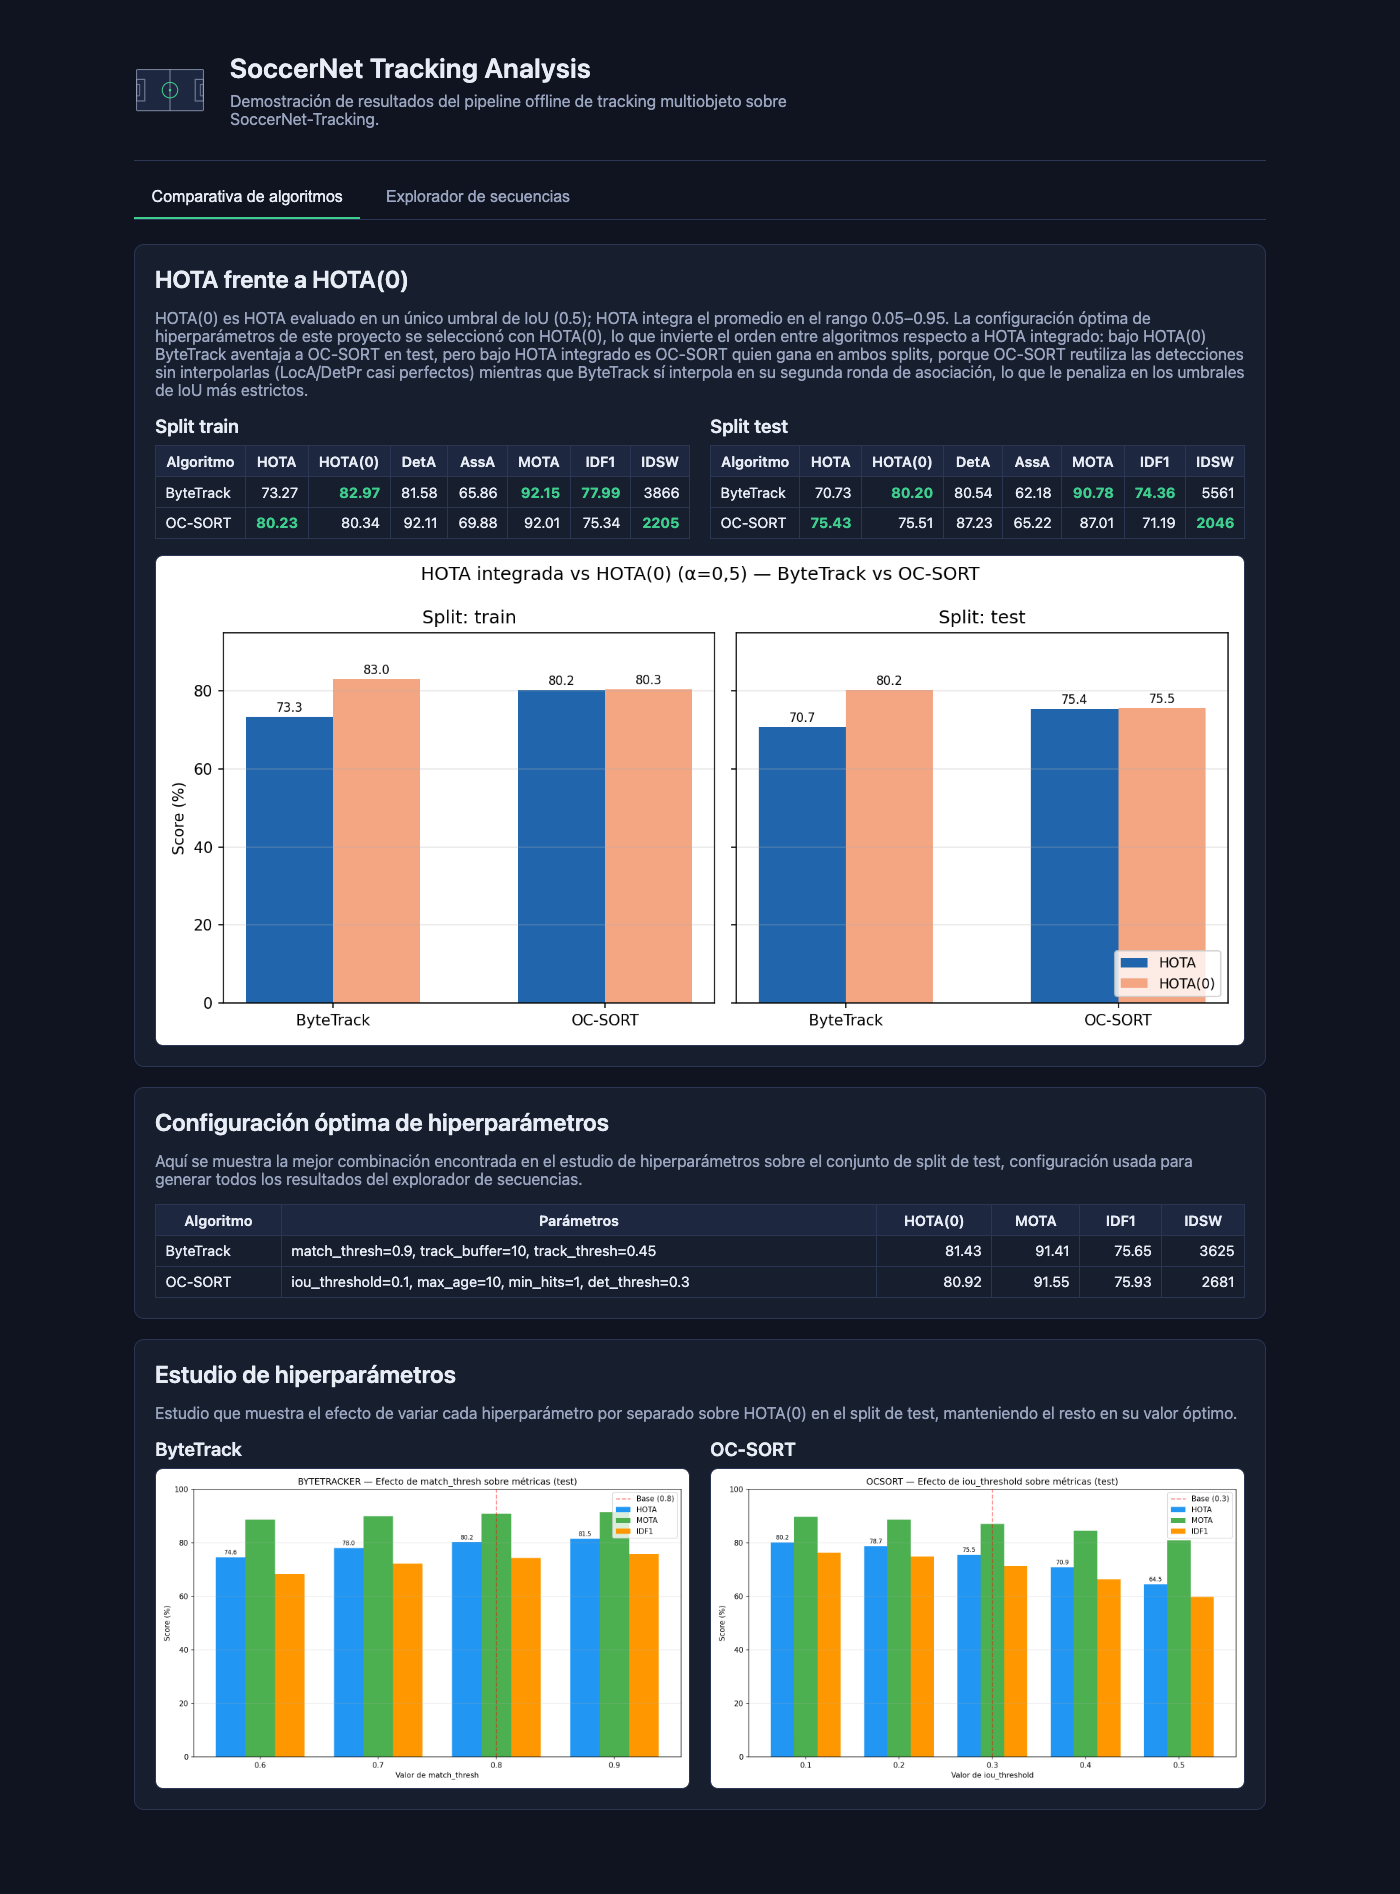
\includegraphics[height=0.8\textheight, keepaspectratio]{figures/manual_web_comparativa.png}
\caption[Pestaña \enquote{Comparativa de algoritmos}]{Pestaña
\enquote{Comparativa de algoritmos}: tabla de métricas por \emph{split},
gráfico HOTA frente a HOTA(0), configuración óptima de hiperparámetros y
gráficas de sensibilidad.}
\label{fig:manual-web-comparativa}
\end{figure}

\FloatBarrier

\paragraph{Explorador de secuencias: selección y vídeo.} Esta pestaña
(Figuras~\ref{fig:manual-web-116} a~\ref{fig:manual-web-118}) exige
elegir primero una secuencia (SNMOT-116/117/118) y un algoritmo
(ByteTrack u OC-SORT) mediante los selectores de chips de la parte
superior; el resto de la pestaña se actualiza automáticamente con los
datos de esa combinación concreta, sin recargar la página. El panel de
vídeo reproduce el tramo correspondiente con las cajas delimitadoras
superpuestas, coloreadas por equipo, con el identificador de tracking
de cada jugador y el balón resaltado en un color distinto mediante los
controles estándar de un reproductor, lo que permite comprobar visualmente, frame
a frame si es necesario, la calidad real del tracking sobre el que se
calcula el resto de metadatos.

\paragraph{Clasificación de equipos y posesión.} Debajo del vídeo, el
panel de \textbf{equipos} muestra cuántos jugadores se han clasificado y
el reparto entre Equipo~0 y Equipo~1 para esa combinación concreta, junto con la nota de limitación
sobre el árbitro. El panel de
\textbf{posesión}, a su lado, muestra el porcentaje de posesión de cada
equipo estimado por proximidad al balón.

\paragraph{Mapas de calor y homografía.} El panel de \textbf{mapas de
calor} permite comparar visualmente la ocupación del campo, tanto
general como separada por equipo, sobre la misma escala de color. Cuando la secuencia dispone de
calibración de homografía real,
un panel adicional de \textbf{homografía} muestra el mapa de calor
calibrado en metros reales y una tabla con el top-5 de jugadores por
distancia recorrida, junto con su velocidad media y de pico
(sección~\ref{subsec:diseno-homografia}). La
Figura~\ref{fig:manual-web-117} muestra precisamente el caso en que este
panel no está disponible, con la nota explícita que evita que la
ausencia de datos se confunda con un error de carga.

\begin{figure}[htp]
\centering
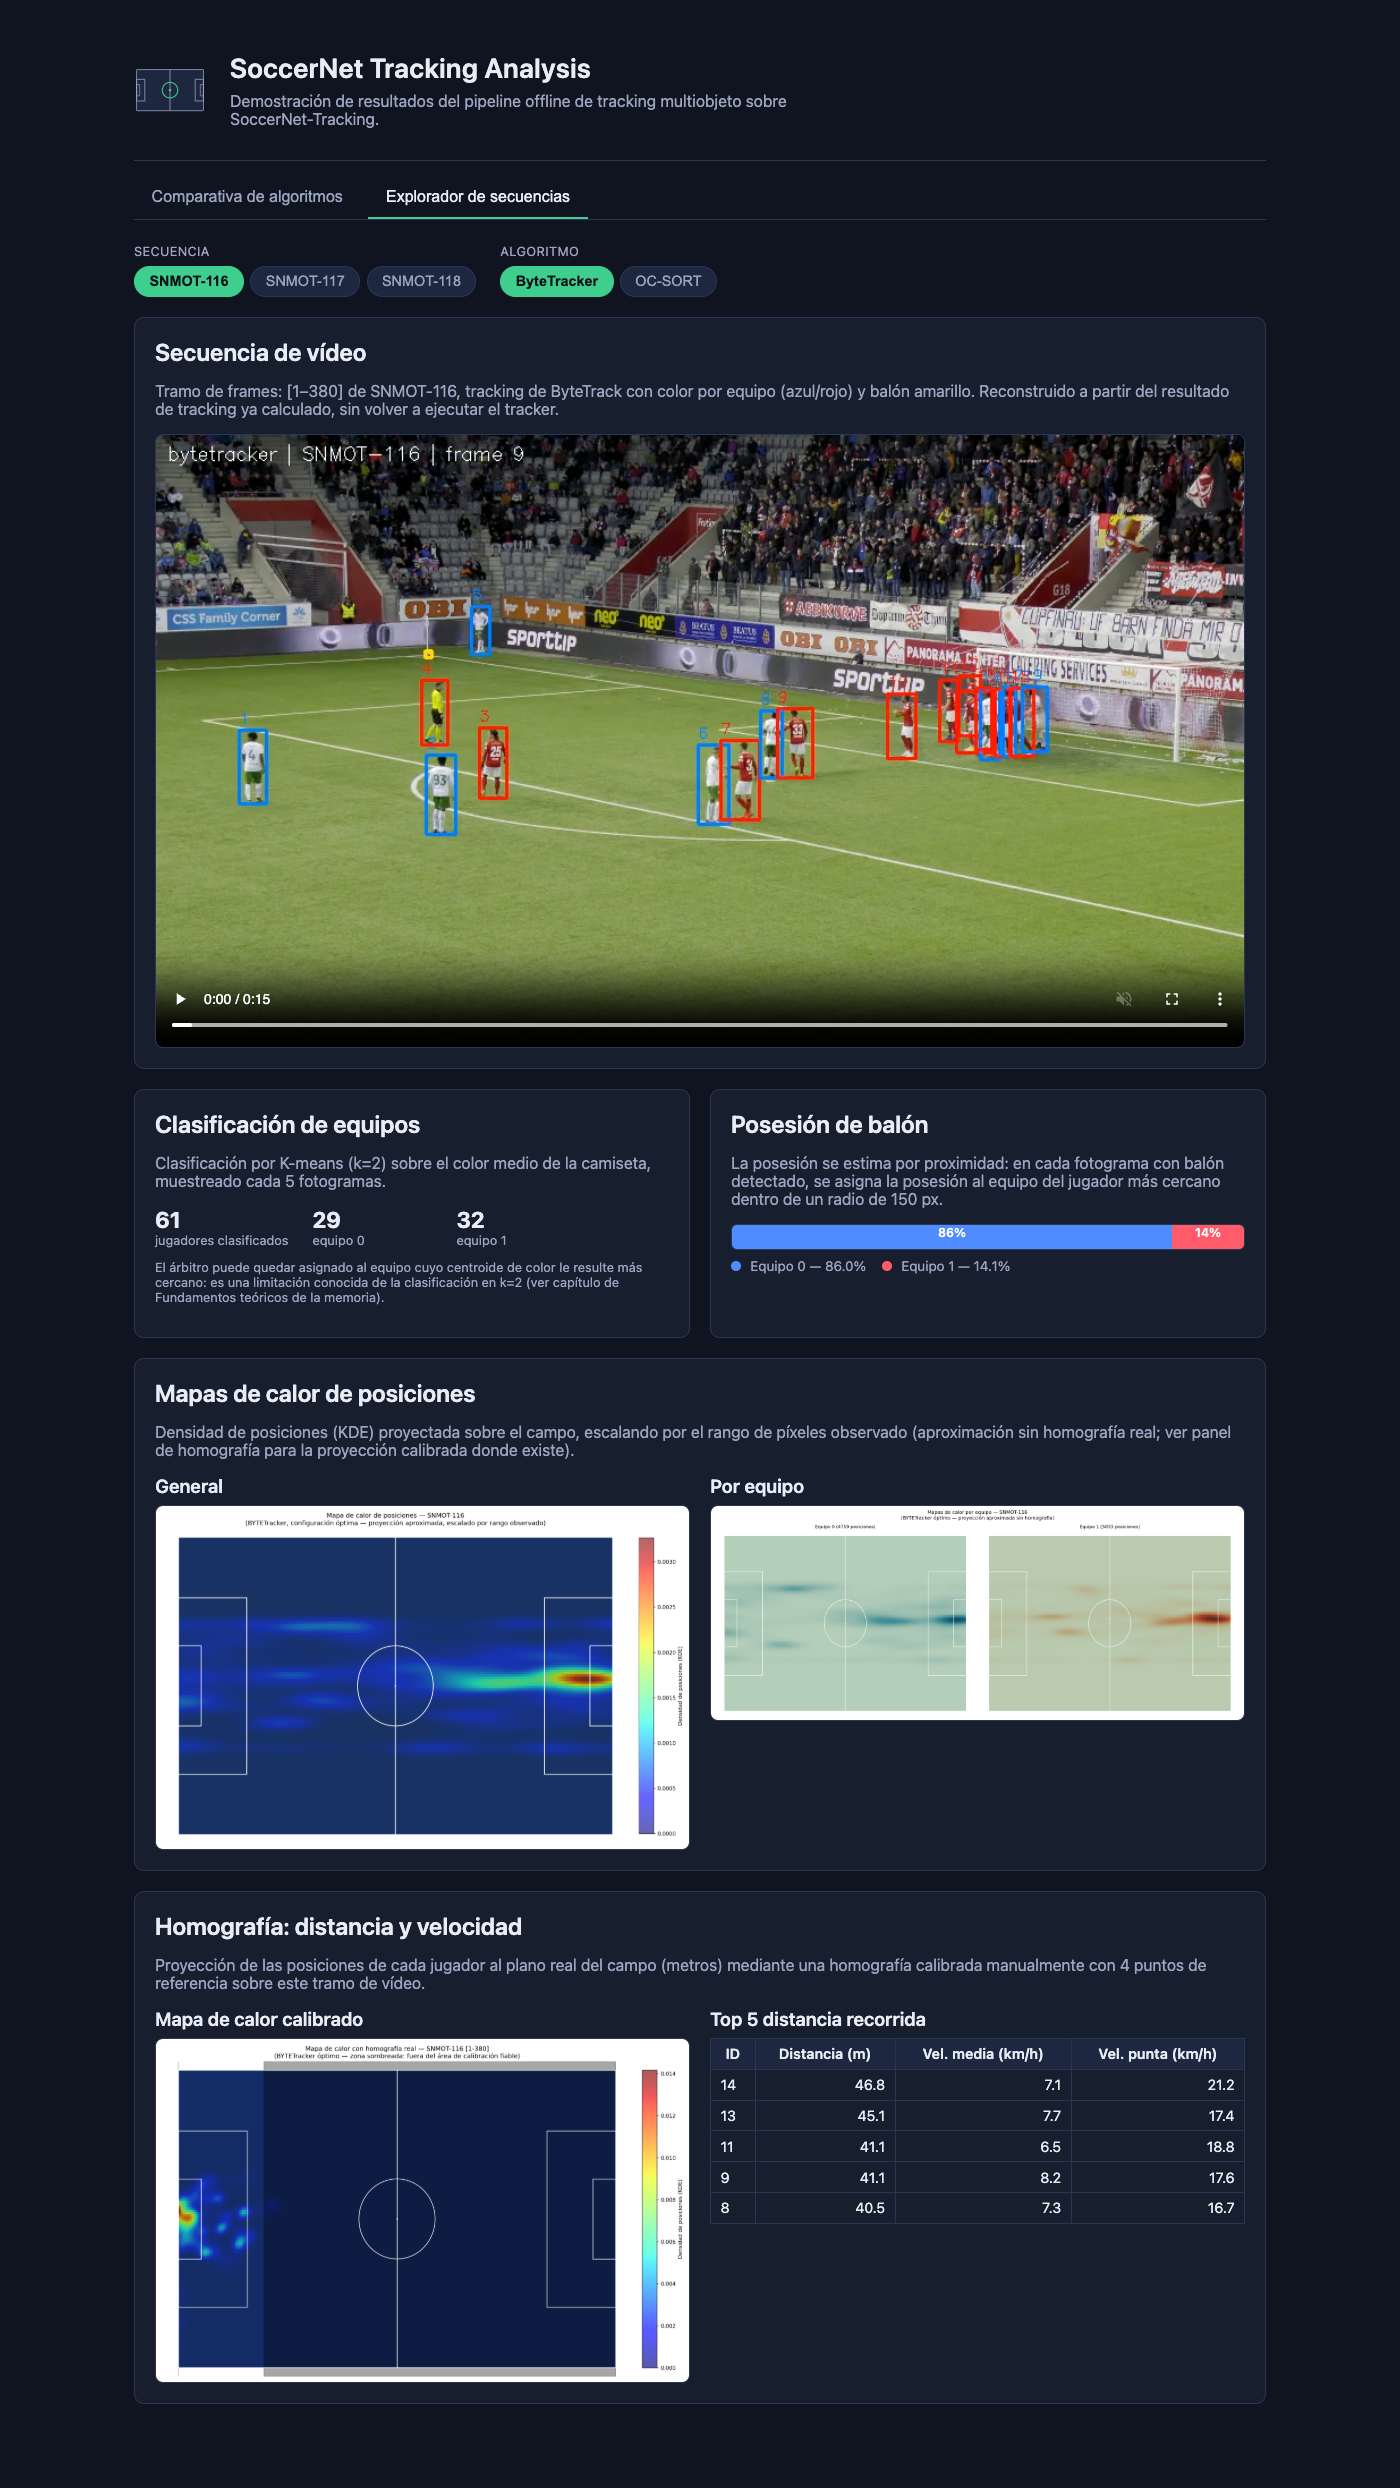
\includegraphics[height=0.8\textheight, keepaspectratio]{figures/manual_web_explorador_116.png}
\caption{Pestaña \enquote{Explorador de secuencias} con SNMOT-116 y
ByteTrack.}
\label{fig:manual-web-116}
\end{figure}

\FloatBarrier

\begin{figure}[htp]
\centering
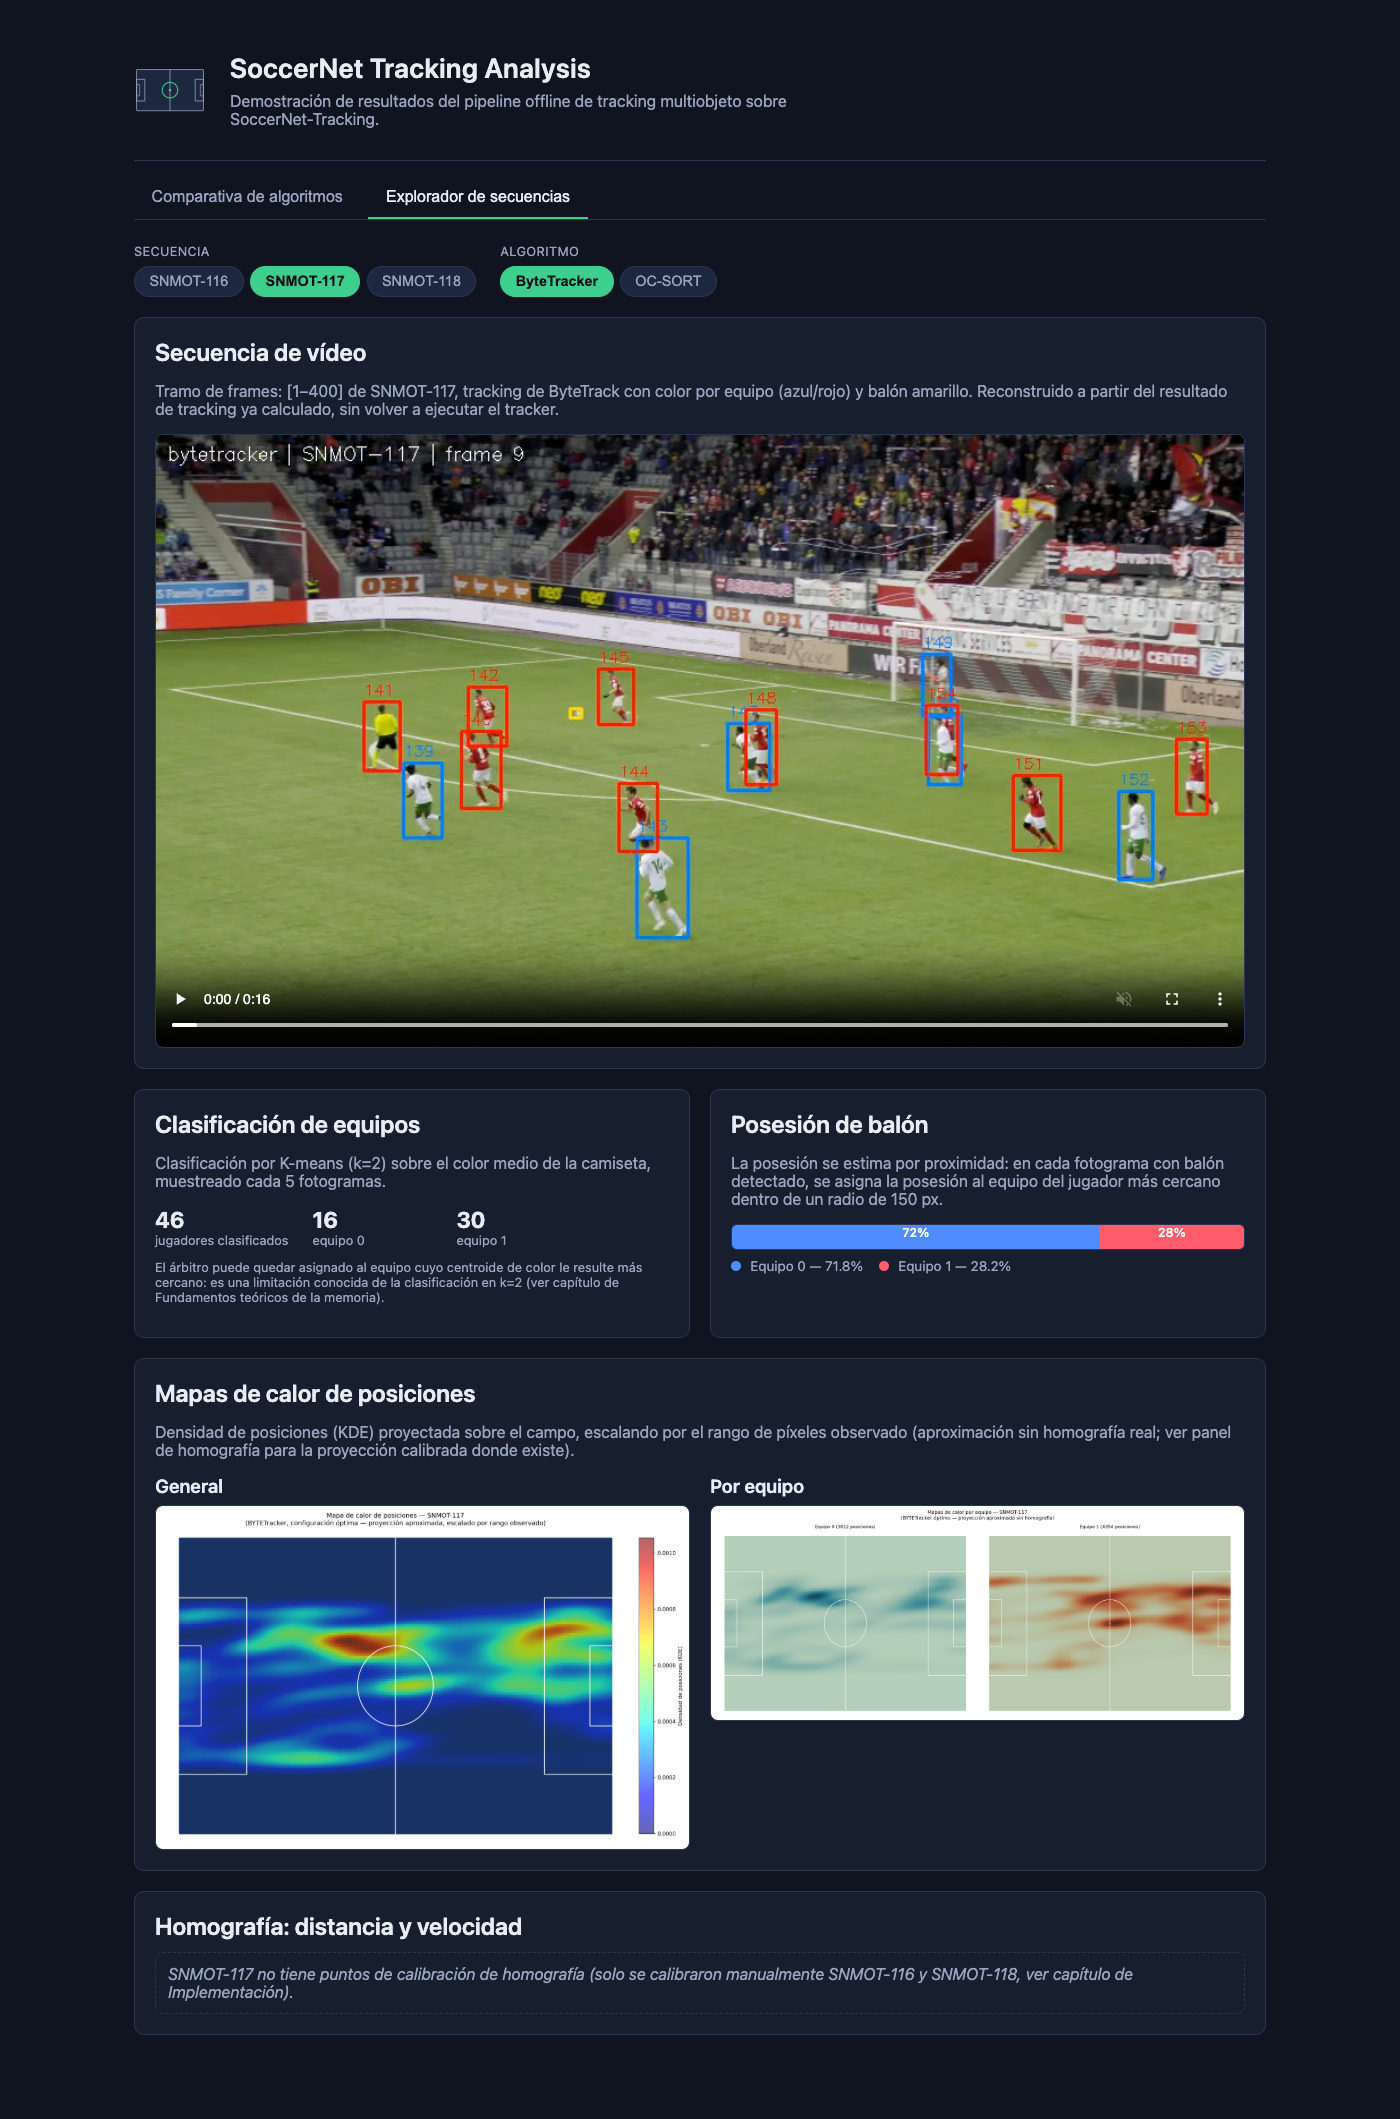
\includegraphics[height=0.8\textheight, keepaspectratio]{figures/manual_web_explorador_117.png}
\caption{SNMOT-117 con ByteTrack.}
\label{fig:manual-web-117}
\end{figure}

\FloatBarrier

\begin{figure}[htp]
\centering
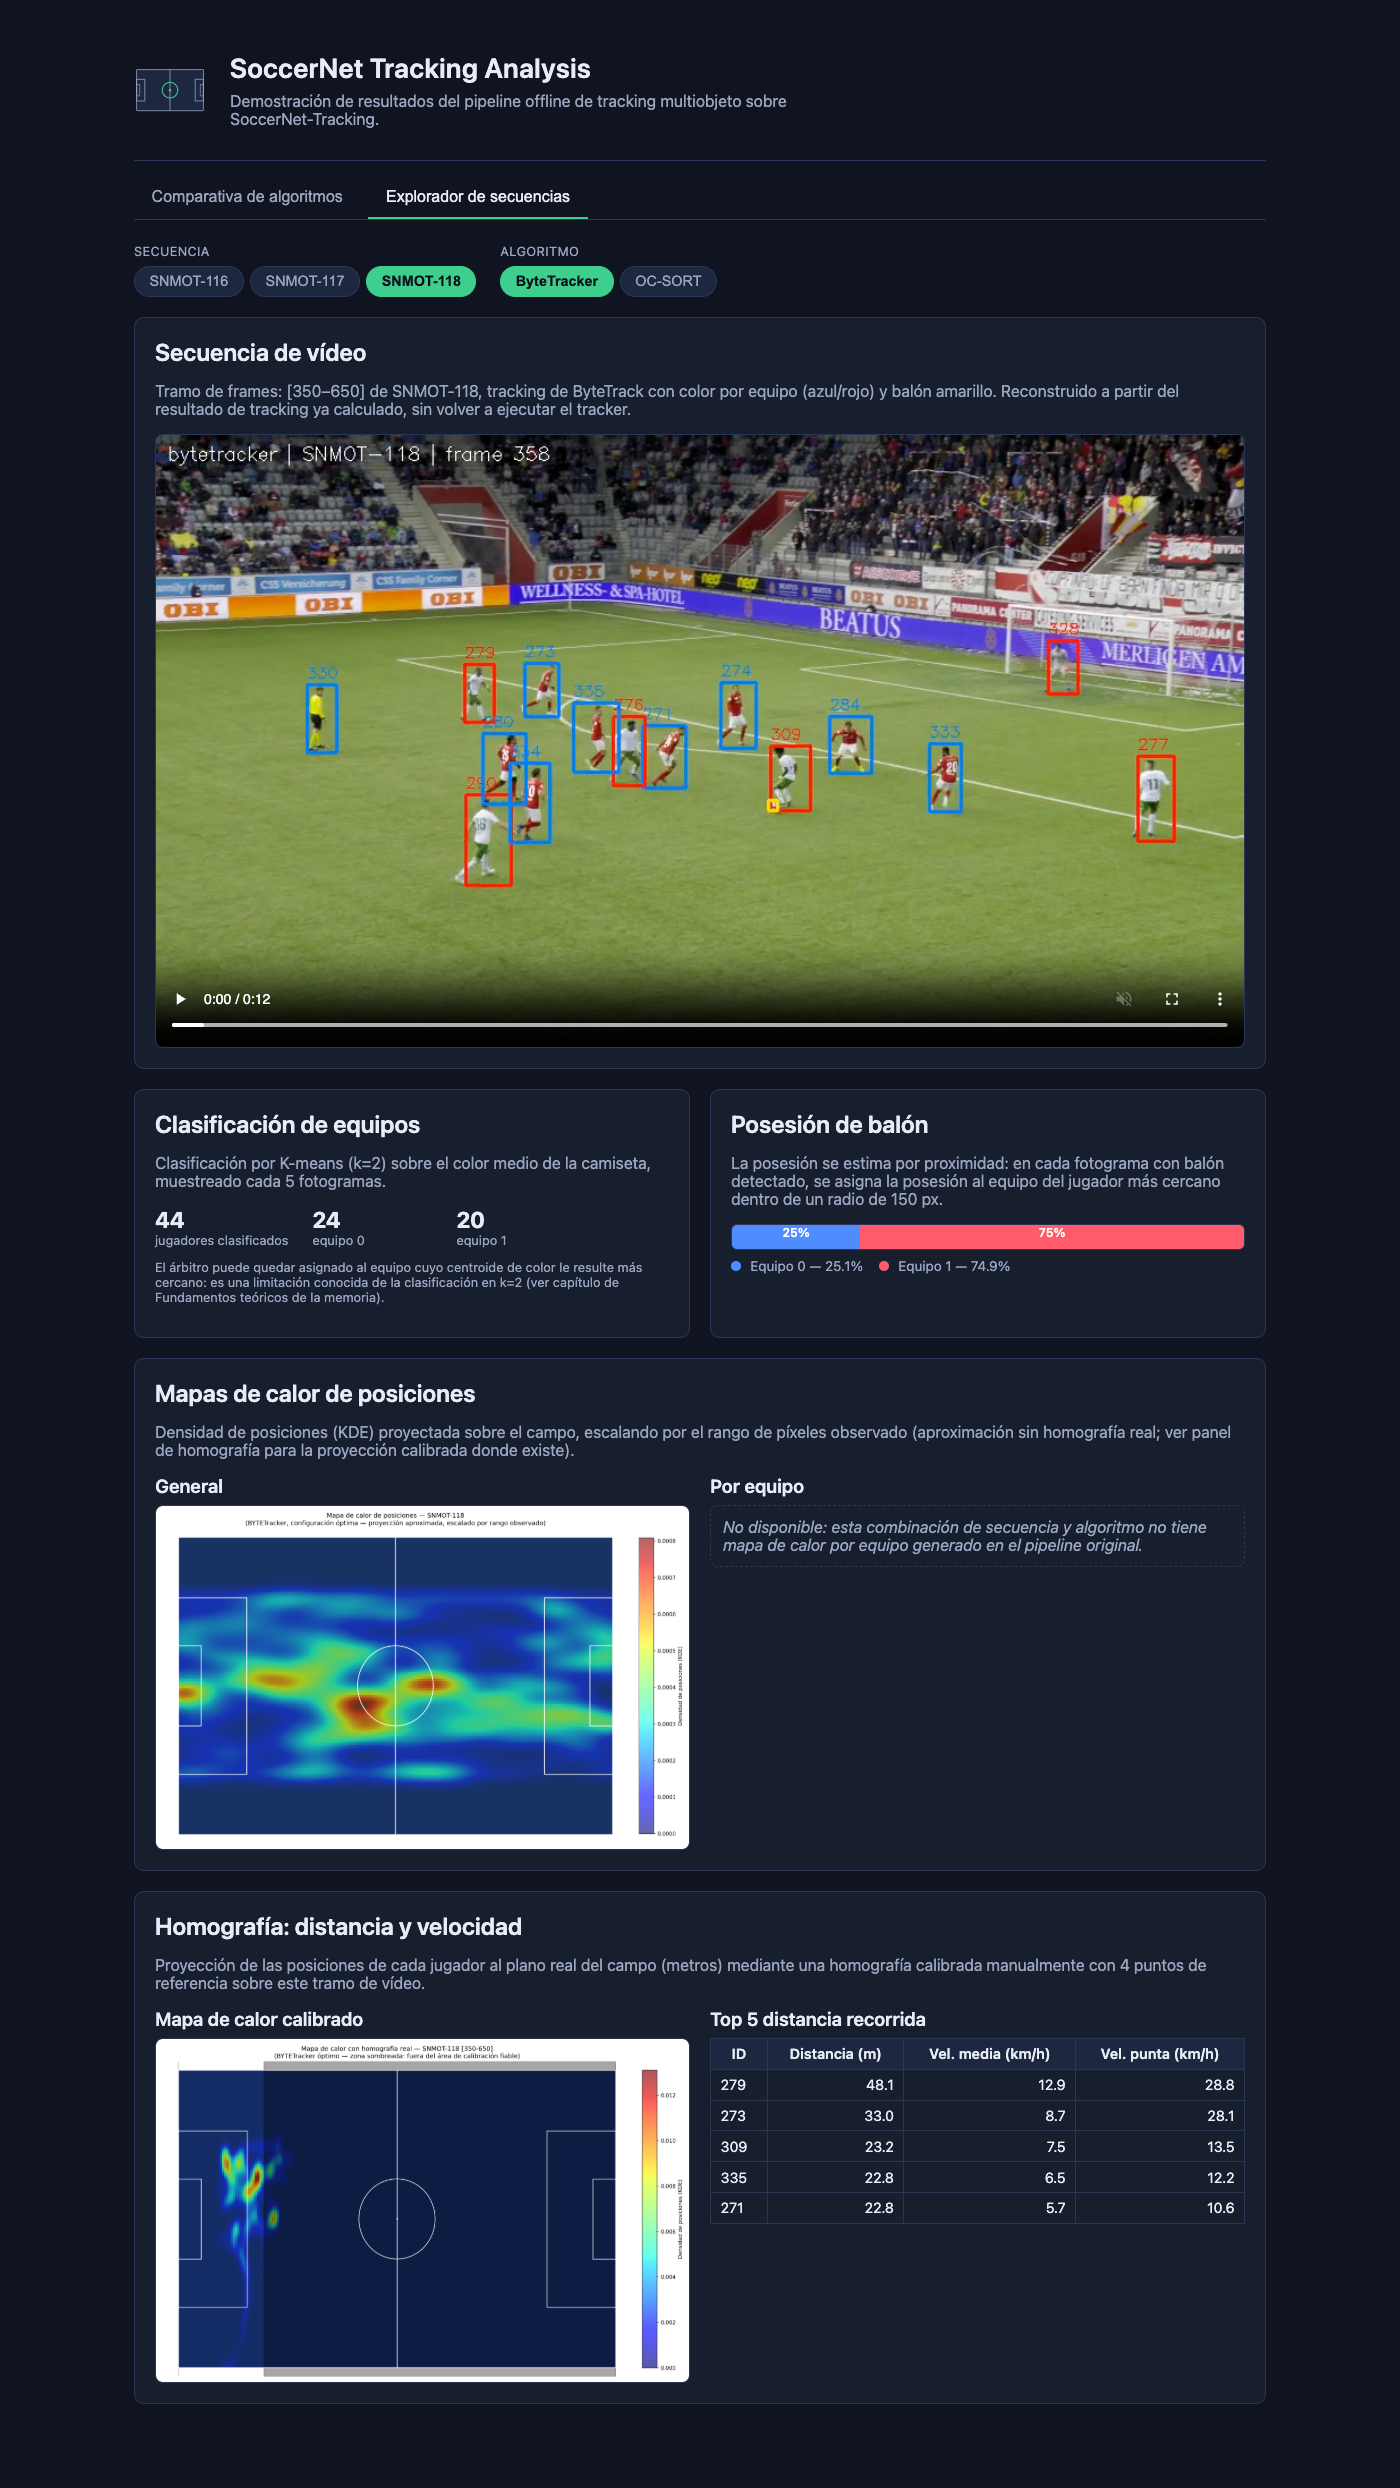
\includegraphics[height=0.8\textheight, keepaspectratio]{figures/manual_web_explorador_118.png}
\caption{SNMOT-118 con ByteTrack.}
\label{fig:manual-web-118}
\end{figure}

\section{Problemas frecuentes}
\label{sec:manual-problemas}

La Tabla~\ref{tab:manual-problemas} recoge, de forma complementaria, los
problemas más probables al desplegar el sistema desde cero siguiendo este
manual, con su causa y solución.

\begin{table}[htp]
\centering
\caption{Problemas frecuentes al desplegar el sistema y su solución.}
\label{tab:manual-problemas}
\renewcommand{\arraystretch}{1.2}
\footnotesize
\begin{tabular}{|p{4.6cm}|p{4.0cm}|p{4.5cm}|}
\hline
\rowcolor{gray!25}
\textbf{Síntoma} & \textbf{Causa} & \textbf{Solución} \\
\hline
\texttt{FileNotFoundError} al leer secuencias del dataset &
  El dataset no está en \texttt{../SoccerNet} relativo al repositorio &
  Clonar el repositorio y descargar el dataset como carpetas hermanas
  (sección~\ref{subsec:manual-dataset}) \\
\hline
Un script de \texttt{src/tracking/} o \texttt{src/metadata/} procesa
  siempre la misma secuencia & La secuencia está hardcodeada en una
  variable al principio del fichero (\texttt{base\_path},
  \texttt{SEQUENCE}) & Editar esa variable antes de ejecutar, o usar los
  scripts \texttt{run\_all\_*.py} para procesar el split completo \\
\hline
\texttt{ModuleNotFoundError: trackeval} al evaluar &
  \texttt{trackeval} no quedó instalado como dependencia transitiva &
  \texttt{pip install trackeval} (sección~\ref{subsec:manual-venv}) \\
\hline
\texttt{heatmap\_by\_team.py} o \texttt{ball\_possesion.py} fallan o dan
  resultados vacíos & No se ejecutó antes \texttt{team\_classification.py}
  para ese algoritmo & Respetar el orden de ejecución de la
  sección~\ref{sec:manual-metadatos} \\
\hline
Los vídeos generados por \texttt{export\_bundle.py} no se reproducen en el
  navegador & \emph{Fourcc} de OpenCV no soportado por navegadores
  (problema P17) & Ya corregido en el código del proyecto
  (\emph{fourcc} \texttt{avc1}); si se modifica el script, mantener ese
  \emph{fourcc} \\
\hline
La pestaña \emph{Explorador de secuencias} no refleja cambios recientes en
  los datos & \texttt{npm run dev} no vigila
  \texttt{frontend/public/data/} & Reiniciar el servidor de desarrollo
  tras regenerar el paquete de datos \\
\hline
\end{tabular}
\end{table}

    \chapter{Uso de inteligencia artificial}
\label{cap:uso-ia}

Durante el desarrollo de este Trabajo de Fin de Grado se utilizaron
herramientas de inteligencia artificial generativa como apoyo al desarrollo
de software, al análisis del código existente y a la redacción de esta
memoria. Este capítulo detalla en qué medida y de qué forma se
han utilizado, siguiendo el mismo criterio de transparencia aplicado al
resto del documento. El uso ha sido sobre distintas áreas del proyecto. Las 
decisiones de diseño y de desarrollo han sido siempre del autor y del tutor
mediante su orientación. Sin embargo, las herramientas de IA han sido un apoyo en la redacción de código y 
resolución de dudas de implementación, así como en la redacción de esta memoria.

\section{Herramientas}
\label{sec:ia-herramientas}

La herramienta empleada ha sido \textbf{Claude Code}.

Conviene distinguir dos usos claramente diferenciados a lo largo del
proyecto, que se detallan en las secciones siguientes:

\begin{itemize}
  \item Como asistente de desarrollo de software, en la
        construcción de la aplicación web y revisor de scripts del pipeline.
  \item Como revisor y en casos redactor partes de esta memoria, a partir de una base del autor y de las notas
         que el autor ha tomado durante el desarrollo del proyecto y del análisis directo del código del
        proyecto.
\end{itemize}

No se ha usado ninguna otra herramienta de IA generativa en ningún punto del proyecto.

\section{Uso en el desarrollo de software}
\label{sec:ia-desarrollo}

El pipeline offline en Python es trabajo previo del autor, desarrollado de
forma independiente antes de emplear Claude Code en este proyecto. En esa
parte, el papel de la herramienta se ha limitado a eer, analizar y corregir o editar
el código ya existente para poder documentarlo con precisión en esta
memoria (sección~\ref{sec:ia-memoria}), no a escribirlo.

El uso de Claude Code como herramienta de desarrollo activo se concentra en
la aplicación web (sección~\ref{sec:implementacion-web}), construida 
durante este proyecto con su ayuda:

\begin{itemize}
  \item El paquete \texttt{src/web\_export/} --\texttt{compute\_metadata.py}
        y \texttt{export\_bundle.py}-- se escribió con Claude Code a partir
        de una instrucción explícita: reutilizar la lógica ya validada de
        \texttt{src/metadata/} sin modificar ni duplicar esos scripts,
        parametrizándola por algoritmo. La verificación de que la lógica
        reproducida era efectivamente equivalente se hizo
        contrastando el código generado contra los scripts originales.
  \item Todo el código de base de \texttt{frontend/} se generó igualmente con Claude Code, a partir de
        decisiones de diseño explícitas del autor: el \emph{stack}
        tecnológico (React, Vite, TypeScript), el alcance del MVP fiel al
        boceto ya planificado en el capítulo~\ref{cap:diseno}, y una ronda
        posterior de ajustes visuales concretos (color de acento, cabecera
        con logotipo, alineación de tablas) solicitados de forma iterativa
        tras revisar la aplicación en ejecución.
  \item Antes de implementar la aplicación web se detectó, durante la fase
        de planificación con la herramienta, un desajuste entre el diseño
        original y los datos realmente disponibles. Se plantearon
        al autor dos alternativas.
  \item Durante la implementación se encontraron y corrigieron con la
        herramienta algunos problemas de implementación, como la incompatibilidad del
        \emph{fourcc} \texttt{mp4v} de OpenCV con la reproducción de vídeo
        en navegador, ya documentada como P17 en la
        Tabla~\ref{tab:impl-problemas}.
\end{itemize}

En todos los casos, el código generado se ha ejecutado y verificado
antes de darlo por válido, no
se ha incorporado código sin comprobar que efectivamente hace lo que se le
pidió.

\section{Uso en documentación}
\label{sec:ia-memoria}

El uso de Claude Code en este proyecto ha sido en gran medida en la redacción y revisión de
esta propia memoria.

La herramienta ayudó en consultar ideas y alternativas para la estructura, la redacción de secciones y subsecciones, la revisión de estilo y
la corrección de errores tipográficos y de sintaxis o reestructurar texto a formato LaTeX.
En ningún caso se ha usado para generar contenido técnico o resultados que no hayan sido verificados por el autor.

Todo con ayuda de una base de memoria que el autor fue construyendo poco a poco y unos documentos 
de notas que el autor fue tomando durante el desarrollo del proyecto con todo detalle y del análisis directo del código del proyecto.

\begin{itemize}
  \item El hallazgo más relevante de todos los detectados durante esta
        redacción es la distinción entre HOTA(0) y HOTA integrada
        : tanto las notas del
        autor como el propio script \texttt{summarize\_hyperparam.py}
        habían usado sistemáticamente la columna \texttt{HOTA(0)} de
        \texttt{TrackEval} bajo el nombre \enquote{HOTA}, lo que llevaba a una
        conclusión que se
        invierte con claridad al recalcular la comparativa con la métrica
        HOTA integrada estándar. Este hallazgo
        no estaba en las notas ni memoria originales: surgió de contrastar el código
        de evaluación con la documentación oficial de \texttt{TrackEval}
        al consultar con Claude la revisión de la parte de métricas en la documentación.
\end{itemize}

\section{Límites del uso de inteligencia artificial}
\label{sec:ia-limites}

Todo el contenido generado con Claude Code ha sido revisado y dirigido por
el autor en cada paso, no aceptado de forma automática:

\begin{itemize}
  \item Los cambios de alcance o de diseño con más de una alternativa
        razonable, por ejemplo, la decisión de generar metadatos de
        OC-SORT en vez de recortar el selector de algoritmo de la
        aplicación web, se plantearon
        explícitamente al autor como una decisión suya, no se resolvieron
        de forma autónoma por la herramienta.
  \item Todos los datos numéricos, tablas y resultados presentados en esta
        memoria proceden de ficheros realmente generados por el pipeline
        del proyecto (\texttt{evaluation\_train/}, \texttt{evaluation\_test/},
        \texttt{evaluation\_hyperparam/}, \texttt{metadata\_output/}), no de
        estimaciones ni de contenido inventado por la IA.
  \item Todo el código generado se ha ejecutado y su salida se ha
        inspeccionado antes de incorporarla a la memoria o de darla por
        válida (sección~\ref{sec:ia-desarrollo}); ningún resultado
        cuantitativo de este documento se ha aceptado sin volver a
        comprobar que procede realmente de la ejecución del sistema
        descrito.
\end{itemize}

En conjunto, el criterio seguido ha sido que Claude Code actúe como
herramienta de apoyo en la redacción y de desarrollo bajo dirección explícita del
autor en algunas decisiones, y que ninguna afirmación de esta
memoria se dé por buena sin haberla contrastado contra una
fuente verificable del proyecto.

    \chapter{Conclusiones y trabajo futuro}\label{cap:conclusiones}

Este capítulo cierra la memoria repasando en qué medida se han alcanzado
los objetivos planteados en el capítulo~\ref{cap:introduccion}, sintetizando
los resultados más relevantes del proyecto, y proponiendo las líneas de
trabajo futuro, algunas de las cuales se han ido señalando a lo largo del documento.

\section{Cumplimiento de los objetivos}
\label{sec:conclusiones-objetivos}

Los once objetivos específicos planteados se han cumplido en su totalidad.

OE-01 a OE-05 el núcleo de la comparación de algoritmos: estudiar el
dataset, implementar ByteTrack y OC-SORT, ejecutarlos sobre la totalidad de
train y test, evaluarlos con las métricas estándar del campo y realizar un
estudio sistemático de hiperparámetros, se han cumplido de forma directa
y están documentados con resultados reales. OE-06 a OE-09
se han cumplido igualmente, con la salvedad, ya señalada en su
momento, de que OE-08 se resolvió como prueba de concepto sobre dos tramos
concretos de cámara estable y no como una solución general al movimiento
continuo de cámara del resto del dataset.
OE-10, documentar de forma
honesta las limitaciones y los enfoques descartados, no es un objetivo que
se cumpla en un capítulo concreto sino un criterio aplicado a todo el documento,
desde la tabla de problemas de entorno del
capítulo~\ref{cap:implementacion} hasta el propio capítulo~\ref{cap:uso-ia}.
OE-11, desarrollar una aplicación web como demostrador visual e
interactivo, se ha completado como un MVP funcional
fiel al diseño planificado en el
capítulo~\ref{cap:diseno}, aunque limitado a las tres secuencias de
demostración usadas a lo largo de la memoria y no al dataset completo.

\section{Resultados principales}
\label{sec:conclusiones-resultados}

Este proyecto como resultado ha dado una comparativa entre dos algoritmos de tracking: ByteTrack y OC-SORT. 
El resultado más relevante de este proyecto no es una cifra aislada, sino la comparativa entre ByteTrack y OC-SORT depende
de forma decisiva de qué variante de HOTA se use para medirla.
Bajo HOTA(0)  ByteTrack
toma ventaja a OC-SORT en el conjunto de test, sin em embargo, bajo HOTA integrada ese resultado se
invierte con claridad en ambos conjuntos, porque OC-SORT reutiliza las
detecciones del \emph{dataset} sin modificarlas mientras que ByteTrack las
interpola en su segunda ronda de asociación, lo que penaliza a ByteTrack en
los umbrales más estrictos que HOTA(0) no llega a evaluar. Son dos formas
igual de buenas para medir el mismo sistema. Que lleven a conclusiones
opuestas sobre qué algoritmo es mejor no es un detalle menor de este
proyecto, es uno de sus resultados.

Sobre la configuración óptima resultante, el pipeline de metadatos
ha demostrado ser aplicable sobre
secuencias reales de SoccerNet, con resultados numéricos consistentes,
por ejemplo, el porcentaje de posesión del equipo dominante en
SNMOT-116 se mantiene prácticamente igual pese a partir de
asociaciones de tracking distintas.

\section{Limitaciones}
\label{sec:conclusiones-limitaciones}

Las limitaciones de este proyecto se han ido documentando a lo largo del desarrollo en
los capítulos del proyecto, pero se resumen aquí:

\begin{itemize}
  \item El estudio de hiperparámetros se realiza en HOTA(0), no en
        la métrica integrada usada en la comparativa principal
        (sección~\ref{sec:pruebas-limitaciones}).
  \item La comparativa de HOTA integrada usa los valores por defecto de
        cada algoritmo, no sus configuraciones óptimas de hiperparámetros
        (sección~\ref{sec:pruebas-limitaciones}).
  \item La clasificación de equipos por K-means con $k=2$ asigna
        incorrectamente al árbitro a uno de los dos equipos
        (sección~\ref{sec:fundamentos-kmeans}).
  \item La homografía real se ha limitado a dos tramos cortos de cámara
        estable, no al dataset completo
        (sección~\ref{sec:implementacion-homografia}).
  \item La posesión de balón es una aproximación por proximidad espacial,
        no una estadística táctica real
        (sección~\ref{subsec:diseno-posesion}).
  \item La detección del balón se basa en un filtro geométrico sobre las
        detecciones del \emph{dataset}, no en un detector entrenado
        específicamente para esa clase.
  \item La aplicación web cubre únicamente las tres secuencias de
        demostración usadas en esta memoria, no el dataset completo para los metadatos.
\end{itemize}

\section{Trabajo futuro}
\label{sec:conclusiones-futuro}

De las limitaciones anteriores, y de los enfoques explorados y descartados
a lo largo del proyecto, se
derivan directamente las líneas de continuación más naturales de este
trabajo:

\begin{itemize}
  \item \textbf{Recalcular el estudio de hiperparámetros con HOTA
        integrada}: repetir el barrido completo de ambos algoritmos
        con la métrica integrada en
        vez de HOTA(0), y evaluar si la configuración óptima resultante
        coincide con la ya encontrada.
  \item \textbf{Evaluar las configuraciones óptimas con HOTA integrada}:
        confirmar si la ventaja de OC-SORT sobre ByteTrack observada con
        los valores por defecto de cada algoritmo se mantiene, se amplía o
        se reduce al usar sus configuraciones óptimas de hiperparámetros.
  \item \textbf{Incorporar algoritmos con re-identificación visual
        (Re-ID)}, como DeepSORT,
        aunque previsiblemente con un margen de mejora menor que en otros
        dominios de MOT, dada la escasa discriminabilidad visual entre
        compañeros de un mismo equipo.
  \item \textbf{Clasificación de equipos con un tercer grupo para el
        árbitro} ($k=3$, combinado con una heurística sobre el tamaño de
        cada grupo), para eliminar el sesgo que introduce actualmente en
        los mapas de calor por equipo y en la posesión de balón.
  \item \textbf{Homografía generalizada y dinámica}, que recalcule la
        matriz de proyección frame a frame para tramos con movimiento de
        cámara continuo, en lugar de limitarse a tramos concretos con
        cámara estática.
  \item \textbf{Extender la aplicación web al resto del dataset}, generando
        el paquete de metadatos y vídeos anotados para más secuencias o
        para su totalidad en lugar de las tres actuales, y explorando un
        detector de balón entrenado que sustituya al filtro geométrico
        actual como base de una posesión más fiable.
  \item \textbf{Tracking sobre un vídeo subido por el usuario}: permitir que
        el propio usuario suba un vídeo de fútbol arbitrario a la
        aplicación web y ejecutar el pipeline de tracking sobre él, en
        lugar de limitarse a las secuencias de demostración ya procesadas.
        A diferencia del resto de este proyecto, que parte de detecciones
        ya calculadas por SoccerNet (sección~\ref{sec:intro-problema}), esta
        vía exigiría incorporar primero un detector de objetos propio, ya
        que un vídeo arbitrario no viene con \texttt{det.txt}. Es
        técnicamente viable con el enfoque ya desarrollado, pero queda
        como línea futura.
  \item \textbf{Participación real en el \emph{leaderboard} oficial de
        SoccerNet}: el dataset incluye un tercer split, \emph{challenge},
        sin \texttt{gt.txt},
        pensado precisamente para enviar resultados al servidor oficial de
        evaluación y obtener una comparación pública y directa con otros
        equipos, en la línea de los ya publicados en ediciones anteriores
        del reto \citep{cioppa2023soccernetchallenges}, ofreciendo esta vez
        una cifra oficial en lugar de la referencia de contexto de la
        sección~\ref{sec:fundamentos-relacionados}.
\end{itemize}

\section{Reflexión final}
\label{sec:conclusiones-reflexion}

Este proyecto partió de una pregunta relativamente acotada
 y ha terminado abarcando un sistema completo, desde el
seguimiento de jugadores hasta la extracción de metadatos deportivos
interpretables y su exposición en una aplicación web. La constatación de que la propia pregunta
\enquote{qué algoritmo es mejor}depende de una decisión metodológica, la métrica
elegida para responderla, que resultó menos trivial de lo que parecía al
principio del proyecto.


    % Bibliografía
    \bibliographystyle{unsrtnat}
    \bibliography{bibliografia.bib}

    % Glosario de términos
    \chapter*{Glosario de términos}
\addcontentsline{toc}{chapter}{Glosario de términos}
\label{cap:glosario}

Este glosario recoge, ordenados alfabéticamente, los términos técnicos y
las siglas usadas a lo largo de la memoria que pueden no resultar
familiares fuera del ámbito del seguimiento multiobjeto y la visión por
computador. Cada capítulo introduce y explica estos conceptos la primera
vez que aparece.

\begin{description}
\item[AssA (\emph{Association Accuracy})] Componente de HOTA que mide la
  calidad de la asociación entre detecciones de un mismo objeto a lo largo
  del tiempo, con independencia de si la detección en sí es correcta
  (sección~\ref{subsec:fundamentos-hota}).

\item[ByteTrack] Algoritmo de \emph{tracking-by-detection} que asocia
  también las detecciones de baja confianza en una segunda ronda, en vez
  de descartarlas directamente (sección~\ref{subsec:fundamentos-bytetrack}).

\item[\texttt{det.txt}] Fichero de detecciones precomputadas de una
  secuencia de SoccerNet-Tracking, en formato MOT: una fila por detección,
  con \emph{frame}, coordenadas de la caja delimitadora y confianza
  (sección~\ref{subsec:fundamentos-soccernet-tracking}).

\item[DetA (\emph{Detection Accuracy})] Componente de HOTA que mide la
  calidad de las detecciones por sí solas, sin tener en cuenta si están
  bien asociadas entre \emph{frames} (sección~\ref{subsec:fundamentos-hota}).

\item[\emph{Fourcc}] Código de cuatro caracteres que identifica el códec
  de vídeo usado al codificar un fichero con \texttt{OpenCV}; el proyecto
  usa \texttt{avc1} (H.264) en vez de \texttt{mp4v} para que los vídeos se
  reproduzcan en el navegador (problema P17,
  Tabla~\ref{tab:impl-problemas}).

\item[\emph{Ground truth}] Anotación de referencia considerada correcta,
  usada para evaluar un sistema; en SoccerNet-Tracking, el fichero
  \texttt{gt.txt} con las posiciones e identidades reales de cada jugador
  (sección~\ref{subsec:fundamentos-soccernet-tracking}).

\item[Homografía] Transformación geométrica que proyecta puntos de un
  plano (la imagen de la cámara) a otro plano (el campo real), usada en
  este proyecto para convertir posiciones en píxeles a metros reales
  (sección~\ref{sec:fundamentos-homografia}).

\item[HOTA (\emph{Higher Order Tracking Accuracy})] Métrica de evaluación
  de \emph{tracking} que combina DetA y AssA, promediada sobre un rango de
  umbrales de IoU (0.05 a 0.95); en este proyecto se distingue
  explícitamente de HOTA(0) (sección~\ref{subsec:fundamentos-hota},
  sección~\ref{subsec:impl-hota-vs-hota0}).

\item[HOTA(0)] Notación usada en esta memoria para el valor de HOTA
  evaluado en un único umbral de IoU (0.5), en vez del promedio integrado
  de la métrica HOTA estándar; la distinción entre ambas es uno de los
  hallazgos centrales del proyecto
  (sección~\ref{subsec:impl-hota-vs-hota0}).

\item[Húngaro, algoritmo] Algoritmo de optimización combinatoria que
  resuelve el problema de asignación óptima entre dos conjuntos, en este
  contexto, qué detección se asocia a qué \emph{track} en tiempo
  polinómico (sección~\ref{subsec:fundamentos-hungaro}).

\item[IDF1] Métrica de evaluación de \emph{tracking} centrada en la
  identidad: mide qué proporción de las detecciones se asocian al
  identificador correcto a lo largo de toda la secuencia
  (sección~\ref{sec:fundamentos-metricas}).

\item[IDSW (\emph{ID Switches})] Número de veces que un algoritmo de
  \emph{tracking} cambia por error el identificador asignado a un mismo
  objeto real (sección~\ref{sec:fundamentos-metricas}).

\item[IoU (\emph{Intersection over Union})] Medida de solapamiento entre
  dos cajas delimitadoras: el área de su intersección dividida entre el
  área de su unión, usada tanto para asociar detecciones como para
  evaluar \emph{trackers} (sección~\ref{subsec:fundamentos-iou}).

\item[K-means] Algoritmo de agrupamiento no supervisado que reparte un
  conjunto de puntos en $k$ grupos según su cercanía; usado en este
  proyecto para clasificar jugadores por equipo a partir del color de su
  camiseta (sección~\ref{sec:fundamentos-kmeans}).

\item[Kalman, filtro de] Algoritmo recursivo de estimación que predice el
  estado futuro de un sistema (aquí, la posición de un jugador) y lo
  corrige con cada nueva observación, base de los algoritmos de
  \emph{tracking-by-detection} usados en este proyecto
  (sección~\ref{subsec:fundamentos-kalman}).

\item[KDE (\emph{Kernel Density Estimation})] Técnica estadística para
  estimar la densidad de un conjunto de puntos de forma continua, usada
  para generar los mapas de calor de posiciones a partir de las
  trayectorias de \emph{tracking} (sección~\ref{sec:implementacion-metadatos}).

\item[MOT (\emph{Multi-Object Tracking})] Seguimiento multiobjeto: la
  tarea de detectar y seguir la identidad de múltiples objetos a la vez a
  lo largo de una secuencia de vídeo, tarea central de este proyecto
  (sección~\ref{sec:fundamentos-mot}).

\item[MOTA (\emph{Multiple Object Tracking Accuracy})] Métrica clásica de
  evaluación de \emph{tracking} que combina falsos positivos, falsos
  negativos y cambios de identidad en un único valor
  (sección~\ref{sec:fundamentos-metricas}).

\item[MVP (\emph{Minimum Viable Product})] Versión mínima funcional de un
  producto, usada aquí para describir el alcance de la aplicación web
  implementada: fiel al diseño planificado, sin todas las ampliaciones
  posibles (sección~\ref{sec:implementacion-web}).

\item[OC-SORT (\emph{Observation-Centric SORT})] Variante de SORT que
  reutiliza las detecciones originales sin interpolarlas y corrige la
  deriva del filtro de Kalman durante oclusiones prolongadas
  (sección~\ref{subsec:fundamentos-ocsort}).

\item[Re-ID (re-identificación)] Técnica que usa la apariencia visual de
  un objeto, además de su posición, para reasociar su identidad tras una
  oclusión; considerada y descartada para este proyecto
  (sección~\ref{subsec:fundamentos-reid}).

\item[\emph{Seqmap}] Fichero que indica a \texttt{TrackEval} qué
  secuencias evaluar en una ejecución
  (sección~\ref{sec:manual-evaluacion}).

\item[SORT (\emph{Simple Online and Realtime Tracking})] Algoritmo
  clásico de \emph{tracking-by-detection} que combina el filtro de Kalman
  con el algoritmo húngaro sobre IoU, base de la que parte OC-SORT
  (sección~\ref{subsec:fundamentos-sort}).

\item[SPA (\emph{Single Page Application})] Aplicación web que carga una
  única página HTML y actualiza su contenido dinámicamente en el
  navegador, sin recargas completas; arquitectura de la aplicación web de
  este proyecto (sección~\ref{sec:diseno-web}).

\item[SoccerNet-Tracking] \emph{Dataset} público de vídeo de fútbol con
  detecciones precomputadas y \emph{ground truth}, usado como base de
  datos de este proyecto
  (sección~\ref{subsec:fundamentos-soccernet-tracking}).

\item[\emph{Split}] Cada una de las particiones del \emph{dataset}
  (entrenamiento, test) sobre las que se ejecutan y evalúan los
  algoritmos por separado (sección~\ref{subsec:fundamentos-soccernet-tracking}).

\item[\emph{Tracking-by-detection}] Enfoque de seguimiento multiobjeto
  que parte de detecciones ya calculadas en cada \emph{frame} y se centra
  en asociarlas entre sí, en vez de detectar y seguir a la vez
  (sección~\ref{sec:fundamentos-tbd}).

\item[TrackEval] Librería de referencia usada en este proyecto para
  calcular HOTA, MOTA e IDF1 de forma estandarizada
  (sección~\ref{sec:implementacion-evaluacion}).

\item[\emph{Tracker}] Nombre genérico para un algoritmo de seguimiento
  multiobjeto; en este proyecto, ByteTrack u OC-SORT.
\end{description}


% Fin del documento
\end{document}
